\documentclass[ngerman,UKenglish,table]{scrbook}

\newcommand*{\texlive}{2009}

%------------------------------------------------------------------------------
\usepackage{ubonn-thesis}
% Glossary package
% \usepackage[acronym,toc]{glossaries}
% TikZ packages and libraries
% \usepackage{tikz}
% \usepackage{tikz-3dplot}
% \usepackage{pgfplots}
% \usetikzlibrary{positioning,shapes,arrows}
% \usetikzlibrary{decorations.pathmorphing}
% \usetikzlibrary{decorations.markings}
\usepackage{thesis_defs}

%------------------------------------------------------------------------------
% Instead of colouring  links, cites, table of contents etc.
% put them in a coloured box for the screen version.
% This is probably a good idea when you print your thesis.
 \hypersetup{colorlinks=false,
   linkbordercolor=blue,citebordercolor=magenta,urlbordercolor=darkgreen
 }

%------------------------------------------------------------------------------
% When writing your thesis it is often helpful to have the date and
% time in the output file. Comment this out for the final version.
%
\ifoot[\today{} \thistime]{\today{} \thistime}

%-----------------------
%Usepackages
%----------------------
\usepackage{bibentry}
\usepackage{booktabs}
%\usepackage[usenames, dvipsnames]{color}
\usepackage{colortbl}
\usepackage{epigraph}
\usepackage{graphicx}
\usepackage{hhline}
\usepackage{listings}
\usepackage{lmodern}
\usepackage{longtable}
\usepackage{multicol}
\usepackage{multirow}
\usepackage[numbers]{natbib}
\usepackage{pdflscape}
\usepackage{printlen}
\usepackage{ragged2e}
\usepackage{rotating}
\usepackage{slashbox}
\usepackage{tabularx}
\usepackage{tabulary}
\usepackage{textcomp}




%\usepackage{amssymb}
%%\usepackage{amsthm}
%\usepackage{array}
%\usepackage{booktabs}
%\usepackage[boxed]{algorithm2e}
%\usepackage{calc}
%\usepackage{colortbl} % colored cells in tables
%\usepackage[utf8]{inputenc}
%\usepackage{diagbox}
%\MakeAutoQuote{“}{”}
%\MakeAutoQuote*{‘}{’}
%\usepackage{enumerate}
%\usepackage{epsfig}
%\usepackage{geometry}
%\usepackage{graphicx}
%\usepackage{hhline} % easy to manage table borders
%\usepackage{hyperref}
%%\usepackage{makeidx}  % allows index generation
%\usepackage{listings}
%\usepackage{lmodern}
%\usepackage{longtable}
%\usepackage{multicol}
%\usepackage{multirow}
%\usepackage[numbers]{natbib}
%\usepackage{pdflscape}
%\usepackage{printlen} % Print lengths using specified units.
%\usepackage{pslatex}
%\usepackage{ragged2e}
%\usepackage{soul}
%\usepackage{subfigure}
%\usepackage[T1]{fontenc}
%\usepackage{tabulary}

%---------------
%User definitions
%---------------

\newtheorem{definition}{Definition}
\newtheorem{example}{Example}


\definecolor{LightCyan}{rgb}{0.88,1,1}
\definecolor{LightYellow}{rgb}{0.96,1,0.88}
\definecolor{LightRed}{rgb}{1,0.88,0.88}
\definecolor{LightBlue}{rgb}{0.88,0.88,1}
\definecolor{LightGray}{rgb}{0.88,0.88,0.88}
\definecolor{Gray}{rgb}{0.7,0.7,0.7}
\definecolor{LightGreen}{rgb}{0.88,1,0.88}
\definecolor{antiquefuchsia}{rgb}{0.57, 0.36, 0.51}
\definecolor{bittersweet}{rgb}{1.0, 0.44, 0.37}
\definecolor{coralpink}{rgb}{0.98, 0.71, 0.67}


\newcolumntype{k}{>{\columncolor{LightCyan}}c}
\newcolumntype{y}{>{\columncolor{LightYellow}}c}
\newcolumntype{d}{>{\columncolor{LightRed}}c}
\newcolumntype{b}{>{\columncolor{LightBlue}}c}
\newcolumntype{e}{>{\columncolor{LightGreen}}c}
\newcolumntype{n}{>{\columncolor{coralpink}}c}

\newcommand\RotText[1]{\rotatebox{70}{\parbox{1cm}{\raggedright#1}}}
\newcommand\Rotatext[1]{\rotatebox{-30}{\parbox{1cm}{\raggedright#1}}}


\newcommand*{\rowstyle}[1]{% sets the style of the next row
  \gdef\@rowstyle{#1}%
  \@rowstyle\ignorespaces%
}


%------------------------------------------------------------------------------
% The following definitions are used to produce the title pages
% needed at various stages
\newcommand{\thesistitle}{Collaborative Authoring of Semantically Structured Multilingual Educational Content}
\newcommand*{\thesisauthor}{Darya Tarasova}
\newcommand*{\thesistown}{Novosibirsk}
\renewcommand*{\InstituteName}{\PI}
\renewcommand*{\inInstitute}{\inPI}
\renewcommand*{\InstituteAddress}{\PIaddress}
% Adjust \thesisreferee...text depending on male/female referee
\newcommand*{\thesisrefereeonetext}{1.\ Gutachter}
\newcommand*{\thesisrefereeone}{Prof.\ Dr.\ S{\"o}ren Auer}
\newcommand*{\thesisrefereetwotext}{2.\ Gutachter(in)}
\newcommand*{\thesisrefereetwo}{Prof.\ Dr.\ X Y}
% Date when thesis was submitted (Master/Diplom)
% Year or Month, Year when thesis was submitted (PhD)
\newcommand*{\thesissubmit}{XX.YY.2015}
% \newcommand*{\thesissubmit}{Month 2013}
% Date of thesis examination (PhD)
\newcommand*{\thesispromotion}{XX.YY.2015}
% Month and year of the final printed version of the thesis
\newcommand*{\thesismonth}{MMM}
\newcommand*{\thesisyear}{2015}
\newcommand*{\thesisnumber}{BONN-IR-2015-XXX}

%------------------------------------------------------------------------------
% The abstract is only needed for the printed version and should be in
% English regardless of the language of the thesis
\newcommand{\thesisabstract}{%
  \begin{otherlanguage}{UKenglish}
    This is your thesis abstract. It may be in a language that is
    different from the rest of your thesis.
  \end{otherlanguage}
}

\newcommand{\myparagraph}[1]{\paragraph{#1} \parskip -5pt \hspace{0pt} \linebreak\RaggedRight}
\newcommand{\firstparagraph}[1]{\paragraph{\large{#1}} \parskip -10pt \hspace{0pt} \linebreak\RaggedRight}
\newcommand{\todo}[1]{\textcolor{red}{@TODO: #1}}

%------------------------------------------------------------------------------
% \includeonly can be used to select which chapters you want to process
% A simple \include command just inserts a \clearpage before and after the file
% Note that \includeonly can be quite picky! Do not forget to put a
% comma after the filename, otherwise it will simply be ignored!
% \includeonly{%
%   thesis_intro,
%   thesis_appendix,
%   thesis_acknowledge
% }

%------------------------------------------------------------------------------
% Give a list of directories where figures can be found. Do not leave
% any spaces in the list and end the directory name with a /
%\graphicspath{%
%  {../figs/},%
%  {../figs/cover/},%
%  {../figs/graphics/},%
%  {../feynmf/}%
%}

%------------------------------------------------------------------------------
% Make a glossary and a list of acronyms
% \makeglossaries

% Glossary entries
% \input{thesis_glossary}

%------------------------------------------------------------------------------





\begin{document}


%\bibliographystyle{plain}
%\nobibliography{biblatex-examples}

\bibliographystyle{plain}
\nobibliography*

% Cover page of thesis - this is only needed for the printed final
% version to be submitted to the department library
% %
% Cover page layout for the department library version
%
% Make the top margin on the cover page larger and also increase the
% size of the left margin to allow for binding. These parameters may
% have to be adjusted if you change the fraction of the page area that
% is used for the text.
% Changing margins works well. Changing the text height has a bad
% effect on the table of contents.
%
{\thispagestyle{empty}
  \addtolength{\oddsidemargin}{1.0cm}\addtolength{\topmargin}{1.0cm}
  \rmfamily\setlength{\parindent}{0pt}
  \begin{center}
    {\fontsize{44}{50}\selectfont
      Universität Bonn}

    \vspace*{20pt}

    \begin{singlespace}
      \fontsize{30}{40}\selectfont
      \InstituteName
    \end{singlespace}

    \vspace*{40pt}

    \begin{onehalfspace}
      \bfseries\huge
      \thesistitle
    \end{onehalfspace}

    \vspace*{20pt}

    {\LARGE
      \thesisauthor
    }
  \end{center}

  \vspace*{\fill}

  \thesisabstract

  \vspace*{\fill}

  {\normalfont\normalsize
    \parbox{0.3\textwidth}{\InstituteAddress}
    \parbox{0.4\textwidth}{%
      \centering
      \includegraphics[width=5cm]{instituts_siegel}
    }
    \parbox{0.3\textwidth}{%
      \thesisnumber\\
      \thesismonth{} \thesisyear\\
      ISSN-0172-8741
    }
  }
}

% %
% Cover page layout for the department library version
%
% Make the top margin on the title page larger and also increase the
% size of the left margin to allow for binding. These parameters may
% have to be adjusted if you change the fraction of the page area that
% is used for the text.
% Changing margins works well. Changing the text height has a bad
% effect on the table of contents.
%
{\thispagestyle{empty}
  \addtolength{\oddsidemargin}{1.0cm}\addtolength{\topmargin}{1.0cm}
  \rmfamily\setlength{\parindent}{0pt}
  \begin{center}
    {\fontsize{44}{50}\selectfont
      Universität Bonn}

    \vspace*{20pt}

    \begin{singlespace}
      \fontsize{30}{40}\selectfont
      \InstituteName
    \end{singlespace}

    \vspace*{40pt}

    \begin{onehalfspace}
      \bfseries\huge
      \thesistitle
    \end{onehalfspace}

    \vspace*{20pt}

    {\huge
      \thesisauthor
    }
  \end{center}

  \vspace*{\fill}

  \thesisabstract

  \vspace*{\fill}

  {\normalfont\normalsize
    \parbox{0.3\textwidth}{\InstituteAddress}
    \parbox{0.4\textwidth}{%
      \centering
      \includegraphics[width=5cm]{instituts_siegel}
    }
    \parbox{0.3\textwidth}{%
      \thesisnumber\\
      \thesismonth{} \thesisyear
    }
  }
}

% %
% Cover page layout for the department library version
%
% Make the top margin on the title page larger and also increase the
% size of the left margin to allow for binding. These parameters may
% have to be adjusted if you change the fraction of the page area that
% is used for the text.
% Changing margins works well. Changing the text height has a bad
% effect on the table of contents.
%
{\thispagestyle{empty}
  \addtolength{\oddsidemargin}{1.0cm}\addtolength{\topmargin}{1.0cm}
  \rmfamily\setlength{\parindent}{0pt}
  \begin{center}
    {\fontsize{44}{50}\selectfont
      Universität Bonn}

    \vspace*{20pt}

    \begin{singlespace}
      \fontsize{30}{40}\selectfont
      \InstituteName
    \end{singlespace}

    \vspace*{40pt}

    \begin{onehalfspace}
      \bfseries\huge
      \thesistitle
    \end{onehalfspace}

    \vspace*{20pt}

    {\huge
      \thesisauthor
    }
  \end{center}

  \vspace*{\fill}

  \thesisabstract

  \vspace*{\fill}

  {\normalfont\normalsize
    \parbox{0.3\textwidth}{\InstituteAddress}
    \parbox{0.4\textwidth}{%
      \centering
      \includegraphics[width=5cm]{instituts_siegel}
    }
    \parbox{0.3\textwidth}{%
      \thesisnumber\\
      \thesismonth{} \thesisyear
    }
  }
}


% Start counting pages from the title page
\frontmatter
% Dedication has to come before \maketitle
 \dedication{For Siberia, which gave me my spirit and for my mom, who taught me how to govern it}

%------------------------------------------------------------------------------
% PhD Title page
% Use this command when you submit your thesis
 %
% Title page layout for submitted version.
%
\title{\thesistitle}
\subtitle{\vspace*{4ex}
  \begin{otherlanguage}{ngerman}
    Dissertation\\
    zur\\
    Erlangung des Doktorgrades (Dr.\ rer.\ nat.)\\
    der\\
    Mathematisch-Naturwissenschaftlichen Fakultät\\
    der\\
    Rheinischen Friedrich-Wilhelms-Universität Bonn
  \end{otherlanguage}
}
\author{%
  vorgelegt von\\
  \thesisauthor\\
  aus\\
  \thesistown
}
\date{}
\publishers{%
  Bonn \thesisyear
}
\lowertitleback{\normalsize
  \begin{otherlanguage}{ngerman}
    Angefertigt mit Genehmigung der 
    Mathematisch-Naturwissenschaftlichen Fakultät der
    Rheinischen Friedrich-Wilhelms-Universität Bonn
  \end{otherlanguage}
  
  \vspace*{10ex minus 4ex}
  
  \noindent
  \begin{otherlanguage}{ngerman}
    \begin{tabular}{@{}ll}
      \thesisrefereeonetext: & \thesisrefereeone\\
      \thesisrefereetwotext: & \thesisrefereetwo\\[2ex]
      Tag der Promotion:      & \\
      Erscheinungsjahr:       & 
    \end{tabular}
  \end{otherlanguage}
}

\maketitle

% Use this command for the print version
% %
% Title page layout for published version
%
% \titlehead{%
%   \centering
%   {\fontsize{44}{50}\selectfont
%     Universität Bonn}

%   \vspace*{20pt}

%   \begin{singlespace}
%     \fontsize{30}{40}\selectfont
%     \InstituteName
%   \end{singlespace}
% }
\title{\thesistitle}
\subtitle{\vspace*{4ex}
  \begin{otherlanguage}{ngerman}
    Dissertation\\
    zur\\
    Erlangung des Doktorgrades (Dr.\ rer.\ nat.)\\
    der\\
    Mathematisch-Naturwissenschaftlichen Fakultät\\
    der\\
    Rheinischen Friedrich-Wilhelms-Universität Bonn
  \end{otherlanguage}
}
\author{%
  von\\
  \LARGE \thesisauthor\\
  aus\\
  \thesistown
}
\date{}
\publishers{%
  Bonn, \thesissubmit
}
\lowertitleback{\normalsize
  \raggedright
  \begin{otherlanguage}{ngerman}
    Dieser Forschungsbericht wurde als Dissertation von der
    Mathematisch-Naturwissenschaftlichen Fakultät der Universität
    Bonn angenommen und ist auf dem
    Hochschulschriftenserver der ULB Bonn
    \url{http://hss.ulb.uni-bonn.de/diss_online} elektronisch
    publiziert.
  \end{otherlanguage}

  \vspace*{10ex minus 4ex}

  \noindent
  \begin{otherlanguage}{ngerman}
    \begin{tabular}{ll}
      \thesisrefereeonetext: & \thesisrefereeone\\
      \thesisrefereetwotext: & \thesisrefereetwo\\[2ex]
      Tag der Promotion: & \thesispromotion\\
      Erscheinungsjahr: & \thesisyear
    \end{tabular}
  \end{otherlanguage}
}

\maketitle


\pagestyle{scrplain}

%------------------------------------------------------------------------------
% You can add your acknowledgements here - don't forget to also add
% them to \includeonly above
%------------------------------------------------------------------------------
\chapter*{Acknowledgements}
\label{sec:ack}
%------------------------------------------------------------------------------

I would like to thank ...

You should probably use \texttt{\textbackslash chapter*} for
acknowledgements at the beginning of a thesis and
\texttt{\textbackslash chapter} for the end.

%%% Local Variables: 
%%% mode: latex
%%% TeX-master: "../mythesis"
%%% End: 


%------------------------------------------------------------------------------
\chapter*{Publications}
%---------------------------------------------------------------------------

This thesis is based on the following journal and conference publications, in which I have been an author or a contributor:


\subsection*{Journal Publications, peer-reviewed}

\begin{itemize}

\item \bibentry{small_journal}.
\item \bibentry{cosmec}.
\item \bibentry{paid_journal}.
\end{itemize}



\subsection*{Conference Publications, peer-reviewed}

\begin{itemize}
\item \bibentry{ekaw_org}.
\item \bibentry{csedu_scoring}.
\item \bibentry{kesw_slidewiki}.
\item \bibentry{csedu_slidewiki}.
\item \bibentry{rdb2rdf}.
\end{itemize}

\subsection*{Book Chapters}


\begin{itemize}
\item \bibentry{russian_book}.
\end{itemize}


\chapter*{Abstract}

\tableofcontents

\mainmatter
\pagestyle{scrheadings}





%------------------------------------------------------------------------------
%==============================================================================
\chapter{Introduction}
\label{chapter:introduction}
%==============================================================================

\epigraph{Knowledge exists to be imparted.}{R. W. Emerson}
\epigraph{The Web does not just connect machines, it connects people.}{Tim Berners-Lee}

\section{Motivation}
\label{section:motivation}

Knowledge expands people’s possibilities.
It promotes creativity and imagination.
In addition to its intrinsic value, it has substantial instrumental value in expanding other freedoms.
Being educated empowers people to advance their interests and resist exploitation.
The worldwide level of literacy has dramatically increased during the 20th century ~\cite{klugman2010human},
both men and women have the right to be educated, and the number of schools worldwide grows constantly.
However, while basic conventional education is accessible for most people around the world, its quality often remains low.
Many people do not have access to a high-quality education due to its high costs, geographical-, language- or cultural barriers.
Overcoming these barriers is one of the most important challenges educators have to face today.

Ensuring the possibility for professionals to educate themselves is another important challenge of today's education programs.
The 21st century reality requires people to continuously acquire new knowledge and skills.
This understanding led to the appearance of the \emph{life-long learning} concept.

Both challenges (barrier-free and life-long education) are addressed by the concept of Open Educational Resources (OER). 
According to the UNESCO definition\footnote{\url{http://www.unesco.org/new/en/unesco/themes/icts/open-educational-resources/}}, OERs are teaching, learning, or research materials that are in the public domain or that can be used under an intellectual property license that allows re-use or adaptation (e.g Creative Commons\footnote{\url{http://creativecommons.org}}).
The OER movement aims to break down barriers that have blocked free access to academic content.
Until recently, most digital educational content was not freely available outside its proprietary institutions.
Moreover, content providers often ensure the materials are protected by passwords and proprietary formats.
The OER movement aims to break down these stratagems, proving that knowledge exchange is beneficial for all participants and society as a whole.
The effort put in promoting these ideas has already been accepted on the highest levels. 
The report from the UNESCO forum on open content for higher education~\cite{unesco} says: "OER represents a major step toward sharing teaching materials, methods, and tools, just as academics have shared their work in scholarly papers for a long time.
The result is to augment teaching resources while expanding knowledge opportunities for learners and faculty members". 

Since the OER strategy has become widely accepted, meeting increasing and increasingly varied demands for high quality education is an important consideration in the policy debate and institutional development in many countries.
It is especially important in the case of developing countries, for whom demand often greatly exceeds capacity in the existing higher education system.

New developments in higher education – from virtual universities and e-learning to open source initiatives – speak to the efforts on the part of the traditional higher education community, as well as new providers, to address this increasing demand.
The open source movement can be seen as reflecting the philosophy of academia, which is based on the sharing of information and new discoveries through the peer-reviewed academic publication process.

Nowadays, open initiatives in education have crystallized around three major areas of activity: the creation of open source software and development tools, the creation and provision of OpenCourseWare (OCW), and the development of standards and licensing tools.
The success of the OER movement depends on the presence of efficient approaches in each of these areas.
While the idea of opening and sharing educational resources is nowadays widely accepted, the OER providers and consumers face significant challenges, such as providing increased access, while containing or reducing costs.
Perhaps the best-publicized and most copied institutional OER model is MIT OpenCourseWare\footnote{\url{http://ocw.mit.edu/}} project.
However, its overall success notwithstanding, the model is hard to follow due to the extremely high costs of development; the project costs approximately \$3.5 million every year, which means the release of each course took an average of 100 working hours.
Furthermore, there is a number of additional challenges preventing the OCW movement from reaching its goals, as summarized in the paragraphs below.

\paragraph{OpenCourseWare and MOOC Initiatives have inherent weaknesses.}
The OpenCourseWare concept arose from the success of open source software by expanding the concept of openness to the educational context.
A vast amount of OCW is being published online to make educational content more easily attainable.
The awareness among users and the popularity of systems providing such courses are increasing.
More than 250 institutions worldwide are openly publishing courses today.
Some OCW initiatives by renowned universities are: MIT OpenCourseWare, Stanford Engineering Everywhere, Carnegie Mellon Open Learning Initiative, Harvard University Extension School, Open Learning Initiative, Initiative, Open Yale Courses, Rice University’s OpenStax, OpenLearn, and Webcast.Berkeley. \todo{links}
Further OCW repositories have been made available by organizations such as: OpenCourseWare Consortium, Open Education Resources Commons, and The Saylor Foundation’s Free Education Initiative.
The Open Education Consortium, the central community of institutions and organizations working on open education, lists 26,611 courses from 80 providers.

However, from a subjective experience, OCW is often cursory, outdated or non-reusable.
Many of the courses contain only a syllabus; are only available in one language; or in formats, which are difficult to reuse.
A systematic analysis~\cite{sahar_vahdati_2015_14756} of 100 courses from major OCW repositories revealed the following weaknesses:

\begin{itemize}
\item{Legal Reusability.} Only 28 out of the 100 courses have a truly open license; the vast majority (i.e. 57 out of 100) are restricting reuse to non-commercial scenarios (i.e. CC-BY-NC-SA), which is not open licensing according to the Open Definition.
If, for example, the courses are offered with a fee or the training organization is a for profit-organization, the non-commercial restriction thus prevents reuse.
\item{Multilinguality.} English is the original language of the vast majority of the courses; only two of which have been translated to other languages.
Only 12 out of the 100 courses were originally offered in languages other than English. 
\item{Format repurposeability.} 68 of the courses are offered in formats supporting some form of repurposeability. However, 52 of these 68 courses are only available in PDF, thereby preventing true reusability.
\item{Recency.} Out of 100 courses assessed in 2014, only 32 courses have been updated in the last two years.
\item{Learning by Self-assessment.} Self-assessment material is only available as part of the course material in 15 courses and separately for another 40 courses.
Out of these 55 courses with some form of self-assessment, just 25 provide solutions.
\item{Engaging course material.} Although, two thirds of the courses have at least one example and one illustration, just one quarter of the courses has more than 50 examples.
Based on the ratio of illustrations per course unit, almost two thirds of the courses are objectively of low attractiveness.
\item{Community Involvement.} The content of 61 courses has been created by a single author. Only 16 courses are the result of collaborative work.
\end{itemize}

\paragraph{Educators are reinventing the wheel every day.}
Despite the plethora of Learning Content Management Systems (LCMS) available and used today, educators are spending most of their time replicating what others have done before.
In the educational domain there is currently no systematic way of sharing and collaborating on content, as is the case in other online domains (e.g. Wikis for text authoring, GitHub~\footnote{\url{http://github.com}} for software development or OpenStreetMap~\footnote{\url{http://openstreetmap.org}} for map creation).
Learning resources are shared only in a cursory way and frequently do not allow repurposing for technical or licensing reasons.
When resources are shared, there is no mechanism to coordinate the synchronisation of various revisions of content (as Wikis, Git or OpenStreetMap allow).
Hence, the maintenance and updating of learning resources is cumbersome and learning resources become quickly outdated.
Furthermore, there is no integrated support for multi-linguality and translation of learning material.

%There is currently a hype around Massive Open Online Courses (MOOCs).
%However, there are two key issues with MOOCs:
%\begin{itemize}
%\item the development and creation of MOOCs is extremely expensive and can easily reach 250-500k Euro without even considering the MOOC delivery cost
%\item MOOCs are only available for relatively few courses covering popular topics and in a limited number of languages
%\end{itemize}

In order to improve this situation and increase the breadth and depth of OpenCourseWare, we have to substantially reduce the effort required for the creation, translation and maintenance of OCW content.
More widely sharing the burden of content creation, translation and maintenance as well as employing crowd-sourcing techniques seems to be a natural candidate strategy for overcoming this obstacle.

\paragraph{Multiplatform learning delivery incorporating LCMS, MOOC.}
Learning Management Systems have dominated e-learning for several years.
They have been widely used by academic institutions for delivering their distance learning programmes, as well as for supporting their students outside the classroom.
They have also been established in the business sector as the mainstream platform for delivering training services to employees.
A Learning Management System (LMS) is an online software application offering facilities for student registration, enrolment into courses, delivery of learning materials to students, student assessment, and progress monitoring.
Popular examples of LMSs used by the academic as well as the business world include \emph{Blackboard}~\footnote{\url{http://blackboard.com}}, \emph{Moodle}~\footnote{\url{http://moodle.org}}, and \emph{CLIX}~\footnote{\url{http://www.im-c.de/germany/en/solutions/learning-management/clix-learning-suite}}.

The emergence of OERs has greatly facilitated online education through the use and sharing of open and reusable learning resources on the Web and via social networks.
Learners and trainers can now access, download, remix, and republish a wide variety of quality learning materials available through open services provided in the cloud.
The emergence of affordable tablet technology has also enabled the mass production and delivery of rich interactive learning materials as eBooks, distributed via popular channels like \emph{iTunes U}~\footnote{\url{https://www.apple.com/education/ipad/itunes-u/ }}.

The OER initiative has recently culminated in MOOCs delivered via providers such as Udacity~\footnote{\url{http://www.udacity.com/}}, Coursera~\footnote{\url{http://coursera.org}} and edX~\footnote{\url{http://edx.org}}.
MOOCs have very quickly attracted large numbers of learners; for example over 400,000 students registered within four months for edX courses.
More recently, the Open University established FutureLearn~\footnote{\url{http://futurelearn.com}} as the UK response to the emergence of MOOCs in collaboration with over 40 organizations (37 universities).
Since its launch, FutureLearn has attracted more than 1 million registered learners worldwide with over 2.2 million course sign-ups. 

These initiatives have led to widespread publicity and also strategic dialogue in the education sector.
The consensus among different groups of stakeholders is that after the web-induced revolutions in communication, business, entertainment, and media, it is now the turn of universities.
Exactly where this revolution will lead is not yet known, but some radical predictions have been made including the end of the need for university campuses, while milder future outlooks focus on ‘blended learning’ (traditional lectures with new digital interactive activities).
Whatever the future might bring, the landscape in higher education is about to change radically.

There is an abundance of systems covering other stages of educational value chains, such as Learning Management (e.g. ILIAS, Moodle, OLAT), Learning Content, Learning Delivery (e.g. OpenCast, FutureLearn), Learning Analytics Systems and social networks.
Instead of trying to incorporate as much functionality as possible in a single system, we need to facilitate the exchange of learning content and educational data between different systems in order to establish sustainable educational value chains and learning eco-systems.
Open (learning meta-data) standards such as SCORM~\cite{scorm_specification2011} are first steps in this direction, but truly engaging, inclusive and multi-lingual value chains can only be realized if we take content structuring to the next level and employ techniques such as interactive HTML5 (which can currently be presented on almost all devices) and fine-grained semantic structuring and annotation of OpenCourseWare.


\section{Problem Definition}
\label{section:problem_definition}

Based on the challenges discussed above, we define the problem addressed by our research as \emph{producing reusable multilingual high-quality educational content with low resources consumption}.
While high levels of quality and reusability can be reached by using models similar to MIT OCW, the issue of decreasing production costs remains mostly unsolved.
Furthermore, if there is a need to offer the content in different languages even more resources are consumed.

An important step towards decreasing the costs, while simultaniously increasing the quality of the educational material, is applying collaborative techniques to the production process.
Such collaboration affects different aspects of content production, such as: content annotation, personalization, and sharing.
According to a study from the early ninetees~\cite{posner1992people}, already at that time most of the work in academia, business and industry was completed by groups of people collaboratively.
This is why collaborative creation of educational materials is natural.
From a psychological and sociological point of view it is proven that people like to collaborate \cite{smith1995cooperative, Halimi2011}.
According to the studies, collaboration positively influences cognitive development in people.
Generally, people even \emph{prefer} to work together; 
according to \cite{smith1995cooperative, Halimi2011}, the reasons for this include:

\begin{itemize}
\item benefiting from partner's knowledge;
\item building strong personal relations with others;
\item increasing the work quality by critique and experience exchange;
\item avoiding duplication and redundancy of tasks.
\end{itemize}

If we consider different domains of content creation; collaborative authoring has dramatically improved the efficiency, effectiveness, quality and timeliness of content creation.
For text authoring, for example, Wiki’s are currently prevalent and are used in corporate intranets of large companies as well as by online communities.
In particular, for encyclopedic article creation, Wikipedia has demonstrated how such a large-scale collaborative process can be superior to traditional content creation processes.
Moreover, as shown in~\autoref{fig:slidewiki_place} collaborative content authoring is not limited to textual content.
For geospatial data, for example, OpenStreetMap has shown how a community of a few thousand collaborators can create a value which previously required multi-billion Euro investments.
Likewise, open-source software development platforms, such as SourceForge, Google Code, or recently GitHub, have dramatically improved the effectiveness and efficiency of community collaboration around software source code and facilitated the creation of widely-used software projects such as Linux, Firefox and LibreOffice.

\begin{figure}
\centering
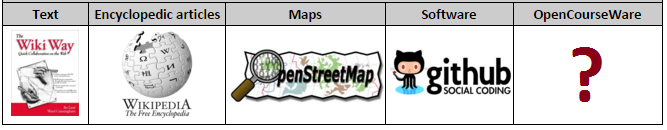
\includegraphics[scale=1]{images/empty_spot.png}
\caption{Collaborative authoring platforms in various domains}
\label{fig:slidewiki_place}
\end{figure}

What all these collaborative platforms have in common is the fact that they were specifically created to support a particular content type.
Wikis support text authoring and versioning; with OpenStreetMap editors, maps can be created; and version control interfaces such as GitHub are tailored for software source-code.
For OpenCourseWare, such technological and organizational support for collaborative authoring and translation does not exist.
To be more specific, there is no authoring tool supporting true collaboration on learning ~\cite{Nurjanah2011}, which should include not only the possibility to reuse (parts of) the content, but also allow authors to understand what other authors do (1), why a learning object should be created (2) and how the authoring process is proceeding (3). 

In order to define the challenges preventing the development of such a system we have conducted systematic literature review in the domain of collaborative authoring of educational content.
The detailed results of this review are presented in~\autoref{chapter:related_work}.
According to our study, the main obstacles for implementing the support of large-scale collaboration on educational content are: 
\begin{enumerate}
\item content reusability and interoperability,
\item full support of social collaboration and
\item support of multilinguality.
\end{enumerate}
The scope of this thesis is to define and discuss these obstacles, as well as propose and evaluate an example system design facing them.

\section{Problem Description and Example Solution}  
Andrea Malupos is a trainer supporting young adults with disability and impairment in their professional life.
At a training center in Madrid, she is training groups of 5-10 school graduates in topics necessary for improving their employment chances.
A particularly important aspect is auto-learning, where the trainees work with the course and accompanying material.
Andrea was requested to prepare a new course module on career development, personal marketing as well as curricula vitae and reference portfolio presentation.
Although she finds some material she could use for her course online, it is cumbersome to investigate licensing conditions, organize and translate the content mostly only available in non-reusable PDF, and enrich it with specific material as well as self-learning and -assessment possibilities.

The solution for the problem would be Andrea becomes part of a national and international network of trainers providing similar training courses.
A collaborative web platform for collaborative OCW authoring is extensively used within the network.
Using the platform, she can quickly develop a structure of the envisioned course material and integrate some existing modules she found.
The colleagues in her network are interested in contributing to specific parts related to their area of competence. 
Using the semi-automatic and crowd-sourced translation features the material is easily translated and kept-in-sync in five languages.
The branching, merging and repurposing features enable everyone to create her own version of the course material, while at the same time benefiting from updates others provide.
Since the material is used by a number of collaborators, new additions and extensions are quickly incorporated into the course and available to everyone.
Andrea's Italian colleague plans to produce a MOOC in Italian on the topic.
Since the course material, including self-assessment questions, tasks, project descriptions, and illustrations, is already available, the effort to produce the MOOC is reduced by more than 60\%.

\section{Research Questions}
\label{section:approach_overview}

The main goal of the research summarized in this thesis is providing a comprehensive approach dealing with the problems of collaborative authoring of OERs.
More specifically, our research answers the following questions:
\begin{enumerate}
\item Related to content reusability: 
\begin{itemize}
\item How to make content reusable on a large-scale?
\item How to make content easy to search and filter?
\item How to publish content with the possibility to migrate it between various platforms?
\end{itemize} 
\item Related to social collaboration: 
\begin{itemize}
\item How to organize and facilitate large-scale collaboration?
\item How to deal with mistakes and vandalism?
\item How to collaborate on structured content?
\end{itemize}
\item Related to multilinguality: 
\begin{itemize}
\item How to decrease the costs of producing multilingual content?
\item How to synchronize content of different language versions?
\end{itemize}
\end{enumerate}


\section{Overview of the Proposed Solution}
In this section we briefly describe the strategies underlying our approach.
Particularly, we give an overview of the concepts we have developed to solve each of three previously defined challenges. 
We address the challenge of content reusability and interoperability by providing innovative WikiApp data model.
In order to facilitate social collaboration on the content we have developed a CrowdLearn concept, based on the WikiApp data model.
To address the multilingual content authoring issue we have extended the CrowdLearn concept to support collaboration on this type of content.
We claim that the resulting CoSMEC concept solves the defined research problem.


\subsection{Content Reusability and Interoperability}
\label{sec:content_reusability_structuring}
The paradigm of \emph{Open Educational Resources} supposes the creation and sharing of reusable and re-purposable learning objects, annotated by standardized metadata.
Only learning objects that satisfy these requirements can be (re-)combined in maintainable high-quality OCW.
In order to achieve high levels of learning objects, searchability, reusability and interoperability of the content has to be structured, annotated by standard metadata, and  published on the web in an efficient manner.
However, the state-of-art approaches in learning objects development and publishing often do not satisfy these requirements.
Usage of different, often proprietary, content formats and system architectures prevents effective migration of content between platforms; lack of structuring makes the repurposing of smaller content pieces impossible; and plain-text metadata limits the searchability.

In order to deal with these issues we propose the use of widely accepted content formats together with generous data models enabling fine-grained content structuring and efficient collaboration on it.
Our approach deals with learning objects in the form of HTML-snippets organized in tree structure.
Each branch of the tree as well as each leaf is an individual learning object annotated by metadata and it can be cut, copied or changed without updating the rest of the tree.
The data model we have developed in order to organize the content in such a way is called WikiApp.
This model supports all operations necessary for collaboration on the structured content; including social networking and version control actions.
In ~\autoref{sec:wikiapp} we introduce this model in detail.
We have chosen HTML format for the content not only because of its generosity, but also because of the recently developed technologies of HTML-content annotating and publishing.
To be published on existing e-learning platforms, the HTML format can be transformed in a number of common e-learning formats automatically or with reasonably low effort.
We have, for example, implemented automatic content transformation into SCORM packages, discussed in more detail in~\autoref{sec:SCORM}.

Content, structured and organized in the way described above, can be transformed into machine-readable formats such as Linked Data.
The Semantic Web and Linked Data movements, with the aim of creating, publishing and interconnecting machine readable information, have gained traction in the last years (cf. \emph{LODStats}\footnote{\url{http://stats.lod2.eu}}).

Making content machine-readable provides a wide list of advantages compared to non machine-readable formats~\cite{khalili2014semantics}:
\begin{itemize}
\item For \emph{search and retrieval}: enriching documents with semantic representations helps to create more efficient and effective search interfaces, such as faceted search~\cite{tunkelang2009faceted} or question answering~\cite{Lopez2011}.
\item In \emph{information presentation}: semantically enriched documents can be used to create more sophisticated ways of flexibly visualizing information, for example by means of semantic overlays as described in~\cite{Burel2009}.
\item For \emph{information integration}: semantically enriched documents can be used to provide unified views on heterogeneous data, stored in different applications by creating composite applications such as semantic mashups~\cite{ankolekar2007two}.
\item To realize \emph{personalization}: semantic documents provide customized and context-specific information, which better fits user needs and will result in delivering customized applications such as personalized semantic portals~\cite{ecs2007}.
\item For \emph{reusability} and \emph{interoperability}: enriching documents with semantic representations (e.g. using the Dublin Core vocabularies\footnote{\url{http://dublincore.org/}}) facilitates content exchange between disparate systems and enables the building of applications such as executable papers~\cite{Muller2011}.
\end{itemize}

In order to perform the transformation we use the RDB2RDF~\footnote{\url{https://www.w3.org/standards/techs/rdb2rdf}} approach, which allows us to convert relational data to a linked data format directly from the database, including the ability to customize the output data model.
We discuss semantic publishing and describe our approach for content conversion in~\autoref{sec:content_migration}.


\subsection{Social Collaboration}

Collaboration on structured educational content can be established within a limited group of experts (1) or involve the power of the crowd (2).
The first approach has a number of issues:
\begin{itemize}
\item It requires a lot of preparation; the domain experts with the knowledge of certain languages have to be found first.
\item Each expert has her own background and point of view on the topic, thus, the negotiations can have a negative effect on the time costs. 
\item It results in production of content available in only a limited number of predefined languages.
\item The content easily becomes outdated; a limited number of experts spread internationally might not be aware of all new findings in the domain.
\item The content refinement is time-consuming and can cause de-synchronization of the content.
\end{itemize}

<<<<<<< HEAD
Since the emergence of the Web2.0 concept, the Internet has transformed from a large-scale source of information into a large-scale collaboration platform.
Following the ideas of Tim Berners-Lee, it is now possible, and even easy, to not only consume information, but to provide and share it through web channels.
Besides, a number of technologies have been developed to support different aspects of this collaboration.
For instance, the wiki-way of content authoring provides tools to make the content creation process accessible for larger audiences while social networking channels support the communication and negotiation of collaborators, as well as allow the sharing of content between users.
These technologies decrease the costs of content development while keeping the content unbiased, up-to-date and open; which are especially important values for educational content.
=======
Since the emergence of Web2.0 concept the Internet has transformed from a large-scale source of information into a large-scale collaboration platform.
Following the ideas of Tim Berners-Lee, it is now possible and even easy not only consume information, but to provide and share it through the web channels.
Moreover, a number of technologies has been developed to support different aspects of the collaboration.
Thus, the wiki-way of content authoring provides tools in order to make the content creation process accessible for larger audience; social networking channels support the communication and negotiation of collaborators, as well as allow sharing the content between users net.
Those technologies allow a decrease in the costs of content development while keeping the content unbiased, up-to-date and open, which are especially important values for the educational content.
>>>>>>> df9f8a0b0ce0852695206c58b57a7b9655e085e6

In our approach we have applied technologies supporting social collaboration to structured educational content development.
In order to do so, we needed to deal with versionning, merging and branching of the structured content, as well as with standard-compliance issues.
To address these challenges we have developed the CrowdLearn concept, presented in~\autoref{sec:Crowdlearn}.
The proposed concept deals with learning objects of fine granularity, allowing their authoring and reuse for all users under a CC-BY-SA~\footnote{\url{https://creativecommons.org/licenses/by-sa/4.0/legalcode}} license.
The license allows reuse, repurpose and updating of the content for anybody as long as the requirement of indicating a list of authors is satisfied.
The structured content is built according to the WikiApp data model, which natively supports social networking actions to engage user negotiation and community building activities.



\subsection{Multilinguality}

<<<<<<< HEAD
The support of multilingual content is crucial for educational platforms because of the many benefits it bring. %what benefits? Be specific
One of the most important benefits of multilingual content is the opportunity to educate without language barriers.
This causes the number of potential learners to increase exponentially with to the number of languages the content is available in.
The learning quality for the previously presented users increases as well, due to the possibility of studying the content in their native language.
Another benefit of multilinguality is the ability to share and exchange knowledge within the multicultural environment.
=======
Nowadays, the support of multilingual content becomes crucial for educational platforms because of the benefits it makes. 
One of the most important benefits of multilingual content supplying is an opportunity to educate without language barriers.
This causes the number of learners to increase exponentially according to the number of languages content is available in.
The learning quality for previously presented users increases as well, due to the possibility of studying in their mother language.
Another benefit of the multilinguality is the ability to share and exchange knowledge within the multicultural environment.
>>>>>>> df9f8a0b0ce0852695206c58b57a7b9655e085e6
This opportunity is crucial for fostering the increase of  education quality, especially in developing countries, where institutes and universities often base courses on outdated information, concepts and theories.
Access to the international scientific knowledge through content synchronization would help experts and educational institutes to be aware of  the current proceedings in their respective fields.

In our approach we propose to use the power of a crowd to author the content available in a number of different languages. 
Aside from other benefits, using crowd-sourcing instead of expert-based translation ensures that the list of available languages is not fixed, but grows with the community size, diversity and activity.
An excellent example of the successful application of crowd-sourcing techniques to multilingual content authoring is Wikipedia~\footnote{\url{http://wikipedia.org}}.
However, the Wikipedia concept does not suppose an (semi-)automatic synchronization of the content presented in different languages.
Although  synchronization is sometimes done manually by contributors, the versions in different languages often remain outdated or even contradictory to each other.

<<<<<<< HEAD
In order to deal with the synchronization issue we have developed the Crowd-sourcing (semantically) Structured Multilingual Educational Content (CoSMEC) concept.
This concept is built on top of the CrowdLearn concept and the WikiApp data model discussed above.
It adds additional relations and operations to model translation activities and connections between original and translated versions.%Too much and, very confusing
The CoSMEC concept introduces the paradigm of \emph{co-evolution} of multilingual content; this entails the ability to update a translation to the current state of the source object and vice versa. 
In this manner, the content versions in different languages can be (semi-)automatically synchronized, while at the same time keeping their status as individual learning objects and thus ensuring their abilities for reuse and repurpose. 
=======
In order to deal with the synchronization issue we have developed the Crowd-sourcing (semantically) Structured Multilingual Educational Content (CoSMEC) concept, described in details in ~\autoref{sec:multilinguality}.
The concept is built on top of CrowdLearn concept and WikiApp data model discussed above.
It adds additional relations and operations to model translating activities and connections between original and translated versions.
The CoSMEC concept introduces the paradigm of \emph{co-evolution} of multilingual content, that means the ability to update a translation to the current state of the source object and vice versa. 
In this manner the content versions in different languages can be (semi-)automatically synchronized, while staying individual learning objects and thus ensuring its abilities to reuse and repurpose.

\section{Research Methods}
As the first step of our research we had to study and formally define existing concepts and strategies facilitating the collaborative authoring in domains other than education.
The results of this work are presented in~\autoref{chapter:technologies_overview}.

In attempt to find existing solutions for the educational domain we have at first conducted a systematic literature study, as discussed in~\autoref{chapter:related_work}.
During the study we have identified the technological and conceptual gaps for some of the issues, as well as collected the best practices and approaches proven to solve other issues.

We have then integrate the existing solutions for particular issues in a comprehensive approach, fulfilling the identified gaps at the same time, as described in~\autoref{chapter:collaboration}.

We implement and evaluate the developed approach with a web-based platform for collaboration on the educational content called SlideWiki.
The implementation details and evaluation results are presented in~\autoref{chapter:implementation}.

During the research we have found out specific issues related to the self-assessment items authoring.
We address the issues in~\autoref{chapter:self_assessment}.

In~\autoref{chapter:conclusion} we conclude our research and give an overview of our future steps.


>>>>>>> df9f8a0b0ce0852695206c58b57a7b9655e085e6

%==============================================================================
\chapter{Collaborative authoring on the Web}
\label{chapter:technologies_overview}
%==============================================================================
\epigraph{(...) people need to be creative. They want to be able to record what they think. They want to be able to, if they see something wrong, go and fix it.}{Tim Berners-Lee}


<<<<<<< HEAD
\todo{introduction}

In this chapter we give an overview of the technologies and paradigms underlying our research.
We will discuss crowdsourcing, social networking and wiki technology.
We will give the (various) formal definitions of the basic terms, as well as summarize the known benefits, limitations and controversies of these paradigms.
=======
In the chapter we give an overview of the technologies and paradigms underlying our research.
Namely, we discuss crowdsourcing, social networking and wiki technology.
We give the (various) formal definitions for the basic terms, as well as summarize the known benefits, limitations and controversies of the paradigms.
>>>>>>> df9f8a0b0ce0852695206c58b57a7b9655e085e6

\section{Crowdsourcing}
Examples of what is now called crowdsourcing can be found far back in the history of humankind.
According to the timeline presented in~\cite{dawson2012getting} the first documented action that can be categorized as crowdsourcing has taken place in 1711 in Great Britain, when the British government was trying to find a way to measure a ship’s longitude.
They offered the public a monetary prize to whomever came up with the best solution, which resulted in collaborative discussion and sharing of ideas between previously unrelated people.

Nowadays, crowdsourcing projects are mostly initiated on web-based platforms.
Although crowdsourcing can be applied to a wide range of tasks, in the scope of our research we focus on the tasks (activities) related to all aspects of content development.
In the next section we will summarize the formal term definitions we rely on and discuss the influence of crowdsourcing on the content development process.


\subsection{Definitions}
\label{sec:crowdsourcing_def}
<<<<<<< HEAD
At present, the specific definitions for crowdsourcing are heavily debated.~\cite{estelles2012towards}
=======
The specific definitions for the crowdsourcing are yet heavily debated~\cite{estelles2012towards}.
>>>>>>> df9f8a0b0ce0852695206c58b57a7b9655e085e6
The word \emph{crowdsourcing} is a compound contraction of \emph{crowd} and \emph{outsourcing}.
Therefore, crowdsourcing can be seen as outsourcing to a crowd, where a \emph{crowd} is a large set of anonymous individuals~\cite{surowiecki2005wisdom}.
Due to anonymity, individuals cannot be individually identified or recognized. 
Implicit in this definition is the idea that a firm cannot “build its own crowd”. 
Moreover, the crowd is generally composed of heterogeneous individuals.
In particular, a crowd may be composed of scientists or experts in various fields, but may also contain of novices.

Crowdsourcing as a business term was coined in 2005 by Jeff Howe~\footnote{\url{http://www.wired.com/2006/06/crowds/}}, who later defined it in his book as shown below.
The term was also defined by the Merriam-Webster dictionary~\footnote{\url{http://www.merriam-webster.com/dictionary/crowdsourcing}}.
We combined both definitions and the word meaning in order to create a more general term, which we will use later in our research (see Definition \autoref{def:crowdsourcing}).

\begin{definition}[By Jeff Howe]
Crowdsourcing is the act of taking a job traditionally performed by a designated agent (usually an employee) and outsourcing it to an undefined, generally large group of people in the form of an open call.
\end{definition}

\begin{definition}[Merriam-Webster dictionary]
Crowdsourcing is the process of obtaining needed services, ideas, or content by soliciting contributions from a large group of people, and especially from an online community, rather than from traditional employees or suppliers.
\end{definition}

\begin{definition}[Combined definition]
\label{def:crowdsourcing}
Crowdsourcing is the process of obtaining needed services, ideas, or content by a form of outsourcing not directed to other companies, but to the large set of anonymous individuals by means of an open call.
\end{definition}

Sometimes it might be challenging to decide if an application can be called a crowdsourcing platform.
In scope of the current research we take into consideration only the systems dealing with digital content. 
In order to define the class of systems we will discuss in this thesis, we adapted the definition from~\cite{doan2011crowdsourcing} to the following:

\begin{definition}[Crowdsourcing system/platform] 
\label{def:cs_system}
A crowdsourcing system is a web-based system that enlists a crowd of people to help solve a problem defined by the system owners; and, in doing so, it addresses the following four fundamental challenges: (1) how to recruit and retain users; (2) what contributions can users make; (3) how to combine user contributions to solve the target problem; and (4) how to evaluate users and their contributions.
\end{definition}

The crowdsourcing activities related to web-based digital content delivery include, but are not limited to:

\begin{itemize}
\item \emph{Creative crowdsourcing}, which spans sourcing creative projects such as graphic design, crowdsourcing architecture, apparel design, movies, writing, illustration, etc.
When applied to the educational domain, the creative crowdsourcing activity can be applied for collaborative authoring of educational content and its metadata.
\item \emph{Crowdsourcing language-related data collection}, which is functionally close to creative crowdsourcing, but requires the crowd to be multicultural.
This special activity is used for creating and improving all kinds of dictionaries.
In \autoref{sec:multilinguality} we discuss the adaptation of this activity for the creation of multilingual educational content and its metadata.
\item \emph{Crowdvoting}, which allows applications to collect opinions and rankings on a certain topic from a large audience.
Crowdvoting may be applied to solve a variety of problems, such as quality assurance, product and services rankings, content recommendations, and others.
In the educational domain we will discuss the crowdvoting activity mostly as an approach for quality management.
\item \emph{Social tagging}, which collects tags for the content, usually in form of notes, questions, labels,  etc. 
These tags are then used for content categorization, search improvements, personalization, and recommendations.
Social tagging allows the transformation of plain text into learning objects with machine-readable metadata. 
\end{itemize}

While these activities are examples of explicit crowdsourcing; a number of approaches to solve a wide range of problems are based on implicit crowdsourcing.
According to \cite{doan2011crowdsourcing}, explicit crowdsourcing entails that users can build artifacts by providing information and editing other people's work.
Users can evaluate particular items like books or webpages, or share by posting products or items.
Implicit crowdsourcing can take two forms: standalone and piggyback.
Standalone allows people to solve problems as a side effect of the task they are actually doing, whereas piggyback takes users' information from a third-party website to gather information.
Implicit crowdsourcing is most frequently used to collect user data in order to apply data-mining techniques to them.
For example, a user's search history can be collected and analyzed in order to discover keywords for ads, spelling corrections, and finding synonyms.
In this way, users are unintentionally helping to improve the performance of existing systems.
Often gamification methods are used to motivate users to implicitly contribute.
For example in the \emph{ESP game}~\cite{von2004labeling}, users guess what is pictured on images and then these labels are used to tag Google images.

\subsection{Benefits, Limitations and Controversies}

Based on definition~\autoref{def:cs_system} alone, it is already clear that crowdsourcing as a task-solving approach has not only benefits, when compared with expert-based approach, but a number of issues and challenges as well.
In comparison to a limited number of experts, a crowd has both strengths and weaknesses.
As was already mentioned in \autoref{sec:crowdsourcing_def}, we focus our later discussion on the content development task.
In this section we discuss the positive and negative influence of crowdsourcing on different aspects of the content development process.

\paragraph{Content quality}

Allowing a community, or even the whole population, to contribute to content creation improves its quality as a result of continuous iterational development, improvement and updating of the content.
Crowdsourcing also positively influences the quality by producing unbiased content due to the incorporation of a large population of participants with diverse backgrounds. 
However, in order for this to be the case, the initiator of the crowdsourcing activity must make sure that the community has enough expertise to solve the task.
Furthermore, the impartiality of the produced content is not absolute.
Research~\cite{hirth2011human} has shown that crowdworkers are a nonrandom sample of the population.
For example, many researchers use crowdsourcing in order to quickly and cheaply conduct studies with larger sample sizes than would be otherwise achievable.
However, due to limited access to internet, participation in lesser developed countries is relatively low.
Participation in highly developed countries is similarly low, because the low amount of pay is not a strong motivator for most users in these countries.
These factors lead to a bias in the population pool towards users in intermediatly developed countries and cause the need to conduct a comprehensive user base study.

Another challence, which calls for the need to study the contributing crowd, is to define a range of possible contributions the users are allowed to make. 
For example, when building a structured knowledge base, users might be allowed to supply attribute-value pairs, correct mistakes and discuss the content structure.
But they can also supply inference rules, resolve controversial issues, and merge conflicting inputs~\cite{richardson2003building}.
Making this strategical decision has a huge impact on the content quality and is crucial for the overall succes of the project.
Moreover, the study of the crowd has to be conducted on a regular basis, as the quality of the crowd might change over time.

Yet another issue is the content consistency, which is the back side of its impartiality. 
Due to the crowd diversity, the content is likely to have inconsistencies in the used terminology or formatting due to the absence of predefined rules.
Besides, the users' background and cultural differences often lead to semantic inconsistency; i.e. when different parts of the same artifact (or its versions in different languages) are based on different assumptions and concepts.  
This is especially true for multicultural crowds and in many cases might not be predicted, even if a comprehensive user base analysis is performed. 
  

%\begin{table}[!ht]
%\centering
%\begin{tabulary}{\columnwidth}{LL}
%\toprule
%
%\textbf{Positive influence} & \textbf{Negative influence} \\
%\midrule
%Potentially unbiased content & Content inconsistency \\
%Up-to-date content & Depends on the size and quality of the user base \\
%Permanent user evaluation & Highly depends on the quality of user base studies \\
%
%\bottomrule
%
%\end{tabulary}
%\caption{Influence of the crowdsourcing on the content quality}
%\label{tab:infl_quality}
%\end{table}


\paragraph{Economical efficiency}

During the iterations, which will eventually lead to better quality content, many unusable and low quality contributions are made as well.
This necessitates sorting and filtering of the contributions, which in turn calls for an increased number of management tasks and therefore staff. 
However, most of the crowdsourcing work is done by people who are either paid or benefit directly from the outcome of the work.
In other cases, the end product is the outcome of a single person's endeavour; one person creates the majority of the product, while the crowd only participates in minor details~\cite{woods2009myth}.

Because the content quality strongly depends on the size and quality of the user base, it is essential to spend a significant amount of the resources on the project dissemination and marketing. 
Additionally, the challenging nature of crowdsourcing requires crowdsourcing systems to be more comprehensive (and therfore more expensive) than systems designed for individual use by a number of trusted experts.

%\begin{table}[!ht]
%\centering
%\begin{tabulary}{\columnwidth}{LL}
%\toprule
%
%\textbf{Positive influence} & \textbf{Negative influence} \\
%\midrule
%Lower costs of content evolution and maintenance & High control and management costs \\
%Fast first results & High costs of marketing and dissemination \\
%No/small need in the user evaluation & High costs of the software design and production \\
% & Need to conduct regular user base studies\\
%\bottomrule
%
%\end{tabulary}
%\caption{Influence of the crowdsourcing on the economical efficiency of the content development}
%\label{tab:infl_efficiency}
%\end{table}

\paragraph{End-user satisfaction}

End-user satisfaction is influenced by choosing crowdsourcing as a basic content development approach.
On the one hand, users can follow the process of content creation from early stages and provide their own opinions and edits.
In that manner the responsibility for the final content quality is shared between content providers and consumers.
Feeling themselves active participants, users will most likely not be disappointed if the process takes more time or resources than planned.
On the other hand, the content development process might seem to the end users a never-ending story.
The content pieces are often at different stages of development, making it hard to predict when the whole planned output will be ready for use.

%\begin{table}[!h]
%\centering
%\begin{tabulary}{\columnwidth}{LL}
%\toprule
%
%\textbf{Positive influence} & \textbf{Negative influence} \\
%\midrule
%Ability to explicitly influence on the result & Never-ending content development \\
%Awareness at all stages &  \\
%
%
%
%\bottomrule
%
%\end{tabulary}
%\caption{Influence of the crowdsourcing on the end-user satisfaction}
%\label{tab:infl_user}
%\end{table}

\section{Web 2.0 and Social Networking}

<<<<<<< HEAD
Already since the time of the World Wide Web's creation, his founder, Tim Berners-Lee, considered it to be the space for global collaboration.
=======
Already from the time of the World Wide Web invention, his inventor Tim Berners-Lee considered it to be the space for global collaboration.
>>>>>>> df9f8a0b0ce0852695206c58b57a7b9655e085e6
In one of his interviews~\footnote{\url{http://www.ibm.com/developerworks/podcast/dwi/cm-int082206txt.html}}, he says: ``\emph{(...) I really wanted it to be a collaborative authoring tool. And for some reason, it didn't really take off that way.}''
Only around ten years after that did we first start to see web sites whose content could be changed by its users.
First, only a small portion of administrators could edit the content of a page through the administration board.
Later, systems allowed users to have their own pages and have administrative rights as well.
This has made it possible for common users to write down and share their thoughts within blogs and bulletin boards.
And finally, social interaction tools, allowing community building and instant communication between users within a group, have made it possible to author content collaboratively.

In this section we give an overview of the concepts behind these social interaction tools, which have transformed the static read-only Web (Web 1.0) into dynamic writable Web (Web 2.0).

\subsection{Definitions}

The term \emph{Web2.0} first appeared in~\cite{dinucci1999fragmented}, however the modern meaning was established and popularized due to the annual \emph{Web 2.0 Summit}~\footnote{originally known as the Web 2.0 Conference} started in 2004.
%the term first appeared in what? Don't just give a number, say what it is, e.g. appeared in the article by ...
Since then, the concept of Web2.0 has been growing and developing.
New technologies and web-based applications have added new meaning to the term and this process is still going on.
Web2.0 can be defined as \emph{writable} or \emph{participative} web, which means that Web2.0 applications and services allow users to use the Internet in a more interactive and collaborative manner, emphasizing peers’ social interaction and collective intelligence~\cite{murugesan2007understanding}.
A conceptual definition of Web2.0 was given by Richard Hall\cite{hall2009towards}
\begin{definition}{Conceptual definition}; Web 2.0 is a second generation, communicative form of the World Wide Web, that emphasizes active participation, connectivity, collaboration, and sharing of knowledge and ideas among its users.
\end{definition}

Although Web 2.0 suggests a "new version" of the World Wide Web, it does not refer to an update of any technical specification, but rather to cumulative changes in the way Web pages are made and used~\footnote{\url{https://en.wikipedia.org/wiki/Web_2.0}}.
Presently, examples of Web 2.0 services include: social networking sites, blogs, wikis, folksonomies, video sharing sites, hosted services, web applications, and mashups.
Based on the research done in the scope of this thesis we formally define Web2.0 as follows:
\begin{definition}
Web2.0 is the complex of Web sites and services allowing and supporting social collaboration on user-generated content.
\end{definition}

Below we explain the terms we used to construct this definition.

\paragraph{User-generated content.} 
The concept of \emph{participative web} supposes wide use of intelligent web services that empower users to contribute to developing, rating, collaborating, and distributing content.
The content created with the use of these services is called \emph{user-generated content}. 
Although the term is self-explanatory, it can be formally defined as follows:
\begin{definition}User-generated content is content which reflects a certain amount of creative effort and is made publicly available over the Internet.
\end{definition}

Most user-generated content activities are undertaken with no expectation of
remuneration or profit.
Motivating factors for creating user-generated content include: connecting with peers, self-expression, and achieving a certain level of fame, notoriety or prestige~\cite{Vickery:2007:PWU:1554640}.
 
\paragraph{Social collaboration.}
The emergency of the Web2.0 concept brought to life the phenomena of social networking sites and platforms.

\begin{definition}[By Educause Center for Applied Research~\cite{educause}]
A Social Networking site is a web-based service that allows to: (1) construct a public or semi-public user profile within a bounded system; (2) articulate a list of other users with whom they share a connection; and (3) view and traverse their list of connections and those made by others within the system.
\end{definition}

These web-based applications were first created to enable large-scale online communication.
Services like Facebook~\footnote{\url{http://facebook.com}}, Google Plus~\footnote{\url{http://plus.google.com}}, Twitter~\footnote{\url{http://twitter.com}}, etc. allow users to establish virtual connections with their real-life friends and users with similar interests.
The distinguishing feature of social networking platforms compared to other communication channels is that communication between users is mostly established through sharing digital materials in the form of textual content and media files.  
Thus, instead of sending private messages, users often share their ideas and opinions publicly, thereby creating and sharing their knowledge.

The developed culture of sharing allows the application of social networking to support a variety of collaborative activities, including content creation (see ~\autoref{fig:social_tools}).
As a result, social networking switched its role from providing a communication channel to supporting large-scale collaboration on the web and became a fundamental tool in any Web2.0 application. 

\begin{figure}[!ht]
\centering
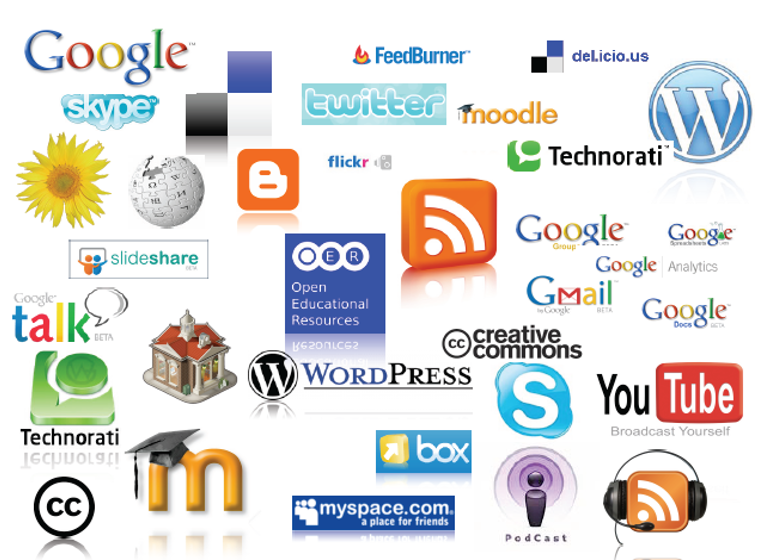
\includegraphics[scale=1]{images/social_media.png}
\caption{Social tools~\cite{rodriguez}.}
\label{fig:social_tools}
\end{figure}



\subsection{Benefits, Limitations and Controversies}

Within the functions of Social Networking the three most beneficial ones for the (educational) content development are~\cite{boyd2007youth}:
(1) support for conversational interaction; (2) support for social feedback; and 
(3) support for social networks and relationships between people

\paragraph{Support for conversational interaction.}
the conversational interaction of users during the content development process is an essential feature of a collaborative authoring tool.
This is especially true for large-scale collaborations, where authors of different cultural and educational backgrounds are involved in the authoring process.
within the scope of our research we are focused mainly on text-based communication channels, but the major principles can be applied to voice- and video- tools as well.
There are two major types of tools enabling communication and discussions between users: 
\begin{enumerate}
\item{synchronous}: text-, voice- and video-chats
\item{asynchronous}: bulletin boards, private and group (instant) messaging
\end{enumerate}

A survey of learning instructors~\cite{branon2001synchronous} showed that both types of comminication tools are preferred for seperate purposes while preparing course materials.
Reasons for using synchronous communication methods included the possibility to implement brainstorming and other team decision-making techniques and dealing with technical issues.
On the other hand, asynchronous communication was found to be more helpful for encouraging in-depth discussion and communicating with temporally diverse colleges, as well as holding ongoing discussions where archiving is required. 
Both types of communication have their disadvantages, however. Disadvantages of synchronous communication include: getting colleges online at the same time, difficulty in moderating large-scale conversations, lack of reflection time for collaborators, and intimidation of poor typists.
Educators also cited the limitations of asynchronous communication: lack of immediate feedback, collaborators not checking in often enough, length of time necessary for discussion to mature, and feeling a sense of social disconnection.

An important requirement for efficient content negotiation, supporting the content development, is that all conversations have to be attached to the exact content piece they refer to.
As a result, if a content piece is being reused or repurposed, the previously discussed questions do not arise again.

\paragraph{Support for social feedback.}
The ability of any reader to leave feedback in an easy and fast way is one of the distinguishing features of social networking sites.
Additionally, the feedback itself (usually only positive) becomes a part of the user-generated content it refers to, letting other users judge the level of quality and actuality of the content.
Sharing "likes" with the peers helps to spread the content that users consider to be interesting and useful, while the content of low interest/quality will be filtered from the users attention. 
An important issue here is the often low level of objectivity of such filtering.
As a result, a piece of content can have a high user rating in one community and be out of interest in another, based on very subjective, "marketing-related" factors, such as attractive illustration or title.

\paragraph{Support for social networks and relationships}
An important feature of Web2.0 is its support of social networks building.

Social network sites allow individuals to: (1)construct a public or semi-public profile within a bounded system; (2) articulate a list of other users with whom they share a connection; and (3) view and traverse their list of connections and those made by others within the system.~\cite{JCC4:JCC4393}
These features allow users to build their own network and stay updated on what is happening within the net.
Applied to content development, social networking helps to engage new users to the team through the relations of team-members.
And the other way around, it allows newcomers to find suitable teams and projects by following the activity of chosen users with whom they have a common background and/or interests.
Another application of social networking to content development is the ability to follow not only users, but projects itself.
This allows team-members to track the changes in an easy way, as well as facilitate the stepping-in process for newcomers.


\section{Wiki}
\label{sec:wiki}
The fundamental class of tools for authoring any content on the Web is \emph{Content Management System} (CMS).
These tools provide an environment where creating, editing and managing of multimedia documents can be done in a friendly, reliable and secure manner~\cite{Rivera2010}.
CMSs aim to facilitate the tasks related to web administration of the content production, such as: editors, user communication tools, styling, etc.

The first generation of CMSs aimed to facilitated content development. They were almost exclusively developed to allow inexperienced IT users to develop, organize and publish content on the Web. 
While asynchronous collaboration was achievable, these first systems, like Blackboard or WebCT, did not have sufficient support for truly large-scale collaboration.
This limitation became especially relevant in the educational domain with the emergence and proliferation of the OER movement.
OERs are built on the belief that everyone should have the freedom to use, customize, improve and redistribute educational resources without constraint. 
This requirement is not being satisfied with the conventional CMSs.
In search of better solutions, educators started to research the application of wiki~\cite{LeufCunningham2001} technology to solve the issue of large-scale collaborative content development.


\subsection{Definitions}

In 1995 Ward Cunningham created WikiWikiWeb, the first Wiki space, and he defined the Wiki as "the simplest online database that could possibly work".
%WikiWikiWeb or just WikiWeb
Later, in January 2001, the founders of the Nupedia project, Jimbo Wales and Larry Sanger, decided to use Wiki to develop the encyclopedia project, thereby creating Wikipedia~\footnote{\url{wikipedia.org}}- the biggest Wiki space of the world.

Wiki technology is a combination of two paradigms: crowdsourcing and Web2.0.
The crucial feature of a wiki environment is its focus on user collaboration, which is enabled by adapting the concept of crowdsourcing to web-based (textual) content authoring. 
The Wiki technology allows the site content to be edited in a collaborative way using a simple notation for contents formatting, indexing, and interlinking.
Additionally, wiki platforms incorporate tools for version control of the content, thereby permitting restoration of the pages.

In order for a platform to be called a wiki, it must satisfy the rules established by the community~\cite{Gokcearslan2011}:
\begin{itemize}
\item No single author is in command; Wiki is a tool that forms its own community and provides democratic collaboration.
\item It has a simplified formatting language (mark-up).
\item Its focal point is its content, not appearance.
\item It provides version follow-up, open to all its users.
\item No security procedure or process of user acceptance is needed. Because the processes in wikis are carried out by a community, i.e. a large number of people, observations are fast and efficient. There is however often a user who is responsible for verifying, and if necessary reverting, of the changes made.
\end{itemize}

\subsection{Benefits, Limitations and Controversies}

Since its inception in the early 2000s~\cite{LeufCunningham2001}, wiki technology became an ubiquitous pillar for enabling large-scale collaboration.
Traditional, text-oriented wikis enabled the creation of the largest encyclopedia of human-mankind edited by tens of thousands of volunteer editors -- Wikipedia.
Also, for group collaboration, in corporate intranets or online communities wiki's meanwhile constitute a fundamental base technology.

Like the most of other crowdsourcing applications, Wiki platforms typically support two essential functions – open editing and edit preservation.
Open editing refers to the ability for anyone to easily edit the content on a wiki.
Edit preservation refers to the ability of wikis to retain all edits to and versions of content contained on the wiki.
Taken together, these two features allow users to "roll back" any changes to the wiki and restore content to a previous version.
These two relatively simple capabilities of wikis, individually and in combination, can create a robust and transparent collaborative environment~\cite{kane2009shoemaker}.

Wikis may work best for knowledge building “over time” (through
versions and groups).
The specific of wikis is the iterative process of content (and knowledge) development.
Even having the predefined plan of what has to be done, the scope of work may be extended due to the new collaboratively created knowledge. 
This specific allows wikis to become a perfect tool for collaborative knowledge engineering, especially in situations, where no one can have a full knowledge of the topic.
Thus, the usage of wikis is not only limited to content development, but to collaborative problem solving.
This is enabled by the fact, that wikis allow:
 
\begin{itemize}
\item progressive problem-solving (particularly open-ended problems) and even problem redefinition.
For example, Wikis could work well for communities of practice whose goal is to develop solutions to common problems over time in order to improve practice
\item explaining increasingly diverse and contrary ideas, as well as examining the relatedness of ideas from diverse contexts
\item combining, synthesizing and evaluating definitions and terminology
across disciplines
\item questioning underlying causes and principles
\item critically reading, and responding in a constructive and public way, to others’ work
\item adding both nuance and complexity to concepts in a given field, through systematic engagement and analysis with work produced by more advanced users
\item observing deeply, stereotype less, and avoiding premature
judgment

\end{itemize}

However, Ward Cunningham's wiki paradigm was mainly \emph{only} applied to unstructured, textual content thus limiting the content structuring, repurposing and reuse.
More recently with the appearance of semantic wiki's the concept was also applied and extended to semantic content (cf.~\autoref{sec:state_of_art_reuse})
In many potential usage scenarios, however, the content to be managed by a wiki is neither purely textual \emph{nor} fully semantic.
Often (semi-)structured content (e.g. presentations, educational content, laws, skill profiles etc.) should be managed and the collaboration of \emph{large} user communities around such content should be effectively facilitated.

Another issue with the wiki paradigm is the content maintainability.
Common wisdom has it that the Wikipedia has been created by "the crowd".
However, the analysis of Wikipedia editing processes reveals that bots are 22 of the top 30 most prolific editors and collectively make about 16\% of all edits to the English language version each month~\cite{geiger2011lives}.
Thus, a large wiki-system is not able to perform efficiently without automatizing some of its functions, especially those related to content quality assurance.

One more issue that is illustrated by Wikipedia is synchronization of content presented in different languages.

In the scope of the current thesis we aim to overcome those limitations, by providing an innovative data model, allowing versionning and collaboration on the (semi-)structured multilingual content (see \autoref{chapter:collaboration})



%==============================================================================
\chapter{State of the Art: Systematic Literature Study}
\label{chapter:related_work}
%==============================================================================
The field of educational content authoring is well addressed in the research literature.
In order to obtain the research papers related to our work as fully as possible and filter the unrelated work at the same time we needed to collect only the literature addressing the \emph{collaborative} authoring of reusable educational content.
Such filtering can not be done based only on titles or abstracts, as often from neither of them it is clear if the approach proposed is applicable to collaborative authoring.
From another prospective the full-text reading of the whole scope of the research in the wide and multi-aspect field is not feasible.
We needed a semi-automatic approach to filter the papers from the wide field.

In order to do so, we conducted a comprehensive systematic study of the state-of-art in collaborative authoring of reusable educational materials, 
following a formal systematic literature review process based on the guidelines proposed in \cite{Dyba2007, Kitchenham2004}.

In the chapter we describe the organization of the study, including the research questions we have formulated.
Then we categorize selected papers according to the scope of issues they address and solutions they propose. 
This process results in a mind map for the domain, as well as domain matrix where the major research problems are intersected with technologies and tools that can be applied for their solution.
After that we collect the found terminology important for the field.
And finally, we discuss the most influential approaches for solving the most complicated issues in the domain.

%Additionally, we were motivated by the fact, that although many of the approaches found in the literature were proven to be beneficial, the existing leading OCW authoring platforms do not integrate them.
%We aimed to collect and describe these approaches in order to attract community attention to them.


\section{Organization of the Study and Paper Selection}
\label{section:collecting_studies}


A systematic literature review is an evidence-based approach to thoroughly search studies relevant to some predefined research questions and critically select, appraise, and synthesize findings for answering the research questions at hand.
Systematic reviews maximize the chance to retrieve complete data sets and minimize the chance of bias.
As a part of the review process, we developed a protocol (described in the sequel) that provides a plan for the review in terms of the method to be followed, including the research questions and the data to be extracted.
In this chapter we summarize the results of the systematic literature review we conducted in January 2015. 

\subsection{Research Questions}
\label{sec:researchQuestion}

In order to organize the survey we formulated four main research questions:
\begin{enumerate}

\item \emph{What are the main challenging tasks in collaborative authoring of reusable OCW?}
\item \emph{Which technologies are being used to solve these tasks?}
\item \emph{How well covered are the challenging tasks in the scientific literature?}
\item \emph{What are the main gaps in state-of-art research?}

\end{enumerate}


\subsection{Search Strategy}
\label{sec:searchStartegy}

To cover as many relevant publications as possible, we used the following electronic libraries:

\begin{itemize}
    \setlength{\itemsep}{0pt}
	\item ACM Digital Library
	\item IEEE Xplore Digital Library
	\item ScienceDirect
	\item Springerlink
	\item ISI Web of Sciences
\end{itemize}

Based on the research questions and pilot studies, we found the following basic terms to be most appropriate for the systematic review:

\begin{flushleft}
\begin{enumerate}
    \setlength{\itemsep}{0pt}
    \item \label{itm:crowd} \textit{crowd-sourcing} OR \textit{crowdsourcing} OR \textit{collaboration}
	\item \label{itm:collaborative} \textit{collaborative} OR \textit{collective} 
	\item \label{itm:authoring} \textit{authoring} OR \textit{creation} OR \textit{edit} OR \textit{editing} 
	\item \label{itm:education} \textit{education} OR \textit{educational} OR \textit{learning} OR \textit{e-learning}
	\item \label{itm:content} \textit{content} OR \textit{resources} OR \textit{material} 


\end{enumerate}
\end{flushleft}

To construct the search string, all these search terms were combined using Boolean ``AND"  as follows:

\begin{center}
(\ref{itm:crowd} OR (\ref{itm:collaborative} AND \ref{itm:authoring})) AND \ref{itm:education} AND \ref{itm:content} 
\end{center}

The next decision was to find the suitable field (i.e. title, abstract and full-text) to apply the search string on.
In our experience, searching in the `title' alone does not always provide us with all relevant publications.
Thus, `abstract' or `full-text' of publications should potentially be included.
On the other hand, since the search on the full-text of studies results in many irrelevant publications, we chose to apply the search query additionally on the `abstract' of the studies.
This means a study is selected as a candidate study if its title or abstract contains the keywords defined in the search string.
In addition, we limited our search to the publications that are written in English and are published after 1999, when, according to \cite{dinucci1999design}, "the first glimmerings of Web 2.0 were beginning to appear".


\subsection{Study Selection}
\label{sec:studySelection}

Based on the search query discussed above, we have collected 4904 papers.
The amount of papers found exceeded the expected one.
We have imported the lists of papers received from the libraries into MicrosoftExcel in order to proceed filtering.

The filtering was proceeded as follows:
\begin{enumerate}
\item Remove duplicates by ordering the titles alphabetically and using in-built Excel functions.
\item Filter the titles, keeping only those which imply the conformity of the paper content to the research questions.
Keeping in mind the large number of papers collected, we had to be more exclusive that was originally planned.
As this might result in missing of important papers, we have added additional steps to ensure the presence of all significant papers in the field.
\item Abstract filtering.
\item Full-text filtering (see details below).
\item Enriching from the references in order to ensure the presence of all significant papers in the field. 
The references to be included were selected based on the rules for filtering the titles from the initial scope.
before including the referenced paper, it was ensured that it is not already present in the scope.
\item Filtering "low-level" papers (see details below).
\end{enumerate}

\begin{figure}
\centering
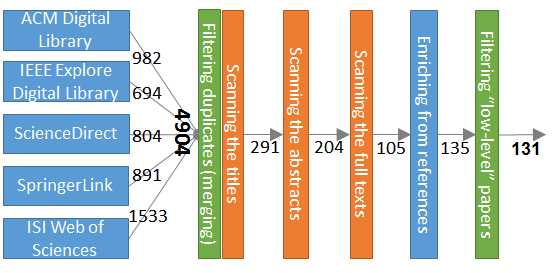
\includegraphics[scale=1]{images/papers_filtering.png}
\caption{Steps followed to scope the search results.}
\label{fig:papers_filtering}
\end{figure}

\paragraph{Details on full-text filtering criteria}
During the scanning of full-text content of the papers we often had to make decisions about including or not-including "borderline" cases.
In the following list we collect the challenges and describe our decisions and their reasons.
\begin{itemize}
\item Some papers discuss the systems not allowing to author new content, but allowing to produce personalized courses out of content added in the repository or on the web.
We have decided to consider such systems not to be OCW authoring tools and thus we do not included papers related to them.
\item In the same manner we do not include papers about tools for collaborative annotation.
\item Even harder was to decide either we should include papers related to collaborative writing tools.
From one perspective, such tools can be used for writing learning text-books with reusable parts, but from another perspective, more often the tools are used for teaching writing or for writing artistic literature.
Another argument to not include this kind of papers is that those tools are usually not complicated technically, their design is quite trivial. 
The papers related to collaborative writing mostly describe use cases and organizational issues. 
In result, it was decided not to include collaborative writing related papers as well.
\item If initially we selected the papers written after 1999, during the filtering we have restricted the criteria and only kept the papers written after 2002.
This is due to the significant difference in the terminology, points of view and challenges addressed.
According to our analysis, we can conclude that Social Web started to influence the educational \emph{research} area only in 2001. 
This can be implicitly proven by appearance of wiki paradigm and Wikipedia in 2001.
\item We have filtered out the papers from the same authors and similar years addressing the same aspects, keeping only the latest or the most detailed one. 
\item We have filtered out the papers of the lowest quality.
Here we did not want to use the quantitative analysis to evaluate the paper quality.
Instead we took our decisions based on several factors important for the study.
\begin{enumerate}
\item In order to be included, the paper should discuss at least one aspect of collaborative OCW authoring in details.
\item If the paper describes an example implementation, the evaluation results have to be provided.
However, the restriction is not applied to the novelty approaches not discussed in any other papers.
\item The approaches proposed should be novel from the technological point of view rather then from pedagogical (however, we kept the papers discussing existing approaches from pedagogical point of view).
\end{enumerate}

\end{itemize}

\section{Paper Categorization and Domain Overview}
In this section we describe our approach to the selected papers categorization.
This process not only facilitates the analyze of the papers we have collected, but as well allows us to build the clear overview of the field itself.

We have processed the categorization in two steps.
The first step of our state-of-the-art analysis was the identification of \emph{aspects} (subdomains or major research problems) of collaborative OCW authoring.
In order to do so we have researched the found surveys and essays.
The analysis of the surveys revealed an absence of comprehensive general survey of the domain, however we reused the results of several surveys and essays for specific aspects, as described in~\autoref{sec:existing_surveys}.
Based on the analysis of the surveys and our background knowledge of the field we have defined the first draft of the domain aspects as depicted in \autoref{fig:initial_map}.

On the next step we classified the rest of the papers into one of aspects representing the main focus of the respective paper.
We refine each aspect with additional sub-branches, thus creating a domain mind map, described in~\autoref{sec:mind_map}.
At the same time we have been filling in a matrix indicating the papers with regard to all aspects and technologies they address.
The matrix discussed in~\autoref{sec:matrix} helps us to identify gaps and promising areas of further research.

\subsection{Analysis of Existing Surveys}
\label{sec:existing_surveys}

As was described above, we have started the papers categorization from selecting surveys and essays we found.
Within the 131 selected papers there were in total 23 surveys, experiment studies and essays related to our topic of interest. 
A significant part of the surveys found is focused only on one particular aspect or technology (e.g "Social Networking" or "Collaborative adaptation authoring").
We incorporated the most important findings of the surveys into the related sections.
The noticeable and influential essays and experiment studies results are discussed/cited mainly in~\autoref{chapter:introduction} and \autoref{sec:Terminology}.

Additionally we found several surveys aimed to answer research questions similar to the ones we defined for the literature study.
However, the here presented analysis of the studies shows the absence of detailed and systematic surveys, and thereby proves the actuality of our research.  

Thus, the study ~\cite{garcia2005educational} in the related work section provides an analysis of the field considering five dimensions: (1) open hypermedia compliant systems, (2) design metaphors used to create the systems, (3) semantic characteristics, (4) collaborative characteristics and (5) adaptive and intelligence characteristics.
The nature of the work however does not allow the authors to present a comprehensive analysis of existing systems (it is not a survey, but system description paper).
Neither does the survey include the latest findings in the field due to its date.

Another review~\cite{Bafoutsou2002} studies the collaborative systems in the understanding of that time. 
This essential study provides detailed functional overview of the systems supporting collaborative work.
The authors define main classes of collaborative systems and classify the studied applications accordingly.
The survey however is not focused on educational materials authoring and is out-dated. 

Several surveys \cite{blau2013collaboration, Strobel2008} discuss pedagogical and sociological aspects of e-collaboration rather than technical.
Thus, in his paper~\cite{blau2013collaboration} the author provides the classification of e-collaboration types, (e.g. synchronous versus asynchronous collaboration, continuous versus one-time contribution approaches etc.).
Due to the nature of the survey, significant attention is paid to user motivation.
The paper is important to understand social behavior of contributors, but addresses the e-collaboration from a different aspect than the current study.

The study~\cite{Luo2010} gives an overview of state-of-art in the collaborative authoring of OCW.
Although the research questions are similar with those of the current study, the approach is different.
The researchers interviewed the end users of the OERs (teachers) and summarized their experiences and the challenges they met.
According to the approach, the study can not be considered systematic.
It is nevertheless important from the practical point of view.
The recommendations given by the authors in the conclusive part however lack technical depth and are too general to be directly incorporated by researches and developers on a technical level.


The rest of surveys and essays addresses specific aspects or technologies of collaborative OCW authoring.
We have summarized all of them in \autoref{tab:survey_1} and \autoref{tab:survey_2}, which were initially defined based on our a priori knowledge of the field, extended and polished with findings from the surveys and essays.

\begin{table}[!ht]


\parbox{.45\linewidth}{
\centering

\begin{tabulary}{0.40\textwidth}{l|l}

\toprule
Concept & Surveys \\
\midrule
\rowcolor{LightGray}
\multicolumn{2}{l}{Authoring paradigms}\\

crowdsourcing & \cite{Moxley2008, Porcello2013}\\
wiki & \\
workflow-based &  \\

\rowcolor{LightGray}
\multicolumn{2}{l}{Semantic Web technologies}\\

semantic wiki & \cite{Pansanato2007, Nesic2010} \\
ontologies &  \cite{Chiribuca2008} \\
RSS-feed &  \\

\rowcolor{LightGray}
\multicolumn{2}{l}{Social networking}\\
activity feed & \\
communication tools & \cite{Bafoutsou2002, Rosmala2012, Nesic2010} \\
social annotation & \cite{Rich2009, Glover2007, Lee2010} \\
social voting & \\
social games & \\
\rowcolor{LightGray}
\multicolumn{2}{l}{Other}\\
AI &  \\
tree-structure & \\
grids, LORs, mash-ups & \cite{Wang2010}\\
\midrule

\textbf{Total}& \textbf{12}\\
\bottomrule
\end{tabulary}
\caption{Surveys and essays studying technologies in application to collaborative OCW authoring}
\label{tab:survey_1}
}
\hfill
\parbox{.45\linewidth}{

\centering
\begin{tabulary}{0.40\textwidth}{l|l}
\toprule
Concept & Surveys \\
\midrule
\rowcolor{LightGray}
\multicolumn{2}{l}{Co-creation}\\
Content authoring & \\
Metadata authoring & \cite{Ola2009} \\
Assessment items authoring & \\
Quality assurance & \\
Categorization & \\
Personalization & \cite{Brusilovsky2003, Chiribuca2008, Lee2010}\\
Localization & \\
\rowcolor{LightGray}
\multicolumn{2}{l}{Reuse and re-purpose}\\
Search, aggregation, filtering  & \\
Remixing & \\
Organization & \\
\rowcolor{LightGray}
\multicolumn{2}{l}{Social collaboration}\\
Negotiation & \cite{Johnson200145}\\
Awareness & \cite{Johnson200145}\\
Network building & \cite{Johnson200145, blau2013collaboration}\\
Engagement & \cite{Johnson200145, blau2013collaboration}\\
\midrule

\textbf{Total} & \textbf{6}\\
\bottomrule

\end{tabulary}
\caption{Surveys and essays addressing the issues of collaborative OCW authoring}
\label{tab:survey_2}
}

\end{table}

\subsection{Analysis of Paper Distribution}

We have continued the paper categorization by building up a domain mind map and domain matrix as discussed below.

\subsubsection{OCW Collaborative Authoring Mind Map}
\label{sec:mind_map}

Our initial mind map constructed after analysis of selected surveys and essays included root branches for 11 concepts, some of which were further branched.
However, as the detailed study of the selected papers has led us to significant changes, we do not illustrate the initial map here, limiting ourselves to a brief discussion of findings made already at this initial step.
The final map is discussed further and presented at~\autoref{fig:super_map}.

The mind map showed the main research trends in the field, as well as underrepresentation of some aspects, which we a priori assumed to be relevant and important to the field.
The distribution of the papers between the concepts is presented at \autoref{fig:initial_map}. 
There is an important assumption here, that each paper is related to just one concept (which is not true in the majority of cases).
This assumption is only initially made at this point for simplifying the usage of the map.


\begin{figure*}[!ht]
  \centering
  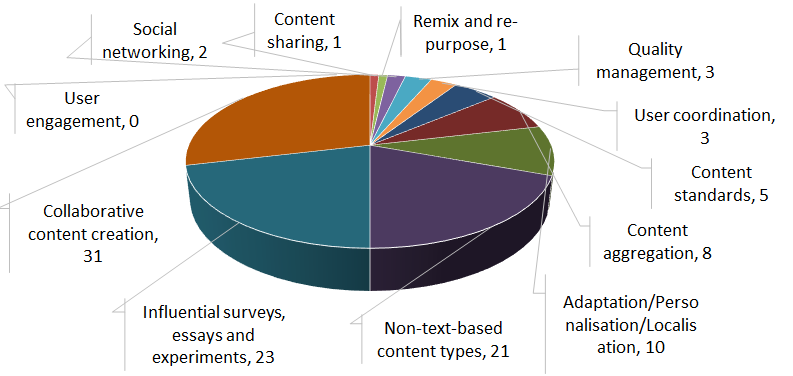
\includegraphics[width=\textwidth]{images/initial_map.png}
  \caption{Distribution of selected papers between a priori identified concepts}
  \label{fig:initial_map}
\end{figure*}

As can be seen on the chart, more than one fifth of the selected papers are surveys essays or case studies (23 articles).
We have separated these papers from the rest as they can not be assigned to any aspect.
As well, we have separated research related to non-text-based content, such as video/audio records, graphics or three-dimensional models (21 articles).
This is due to the significant difference in approaches used to deal with these types of content in comparison with text-based formats.

After separating these two kinds of papers, we observe that the majority of the remaining papers focuses on the aspect of content development using \emph{crowdsourcing} or \emph{wiki} paradigms (31 articles).
The aspects of content adaptation/personalization and content aggregation receive decent attention as well (10 and 8 papers respectively).
Less than 10 percent of the selected papers are focused on any of the other aspects and we could not identify a single paper making its main contribution in the user engagement aspect of the OCW collaborative authoring.

\subsubsection{OCW Collaborative Authoring Matrix}
\label{sec:matrix}

During the detailed analysis of the collected papers we created a matrix indicating the distribution of papers between aspects versus employed technologies.
Again, we do not consider the papers focusing on non-text-based content, as well as surveys and essays. 
The matrix shows the (proposed) use of technologies with regard to the OCW authoring aspects discussed in the selected papers.
Each cell in the matrix includes the papers, in which the technology (indicated in the row) was applied to the aspect (indicated in the column).
As articles usually cover multiple aspects and technologies, they might occur multiple times in the matrix.
Due to the size of the matrix, in the paper we present a simplified version of the matrix in a \autoref{tab:matrix}.
Each cell of the table indicates the count of papers addressing or proposing the application of corresponding technology to a corresponding task.
The total amount of papers considers every paper only once. 


\begin{landscape}
\begin{table}[!b]\scriptsize
\begin{tabulary}{1.3\textwidth}{>{\bfseries}R|e|e|e|e|e|e|e|y|y|y|b|b|b|b|>{\bfseries}n}

\toprule
\multirow{3}{*}{\backslashbox{\Rotatext{Technology}}{\Rotatext{Aspect}}} & \multicolumn{7}{e|}{Content co-creation} & 
\multicolumn{3}{y|}{Reuse and re-purpose} &
\multicolumn{4}{b|}{Social collaboration} & \\

\cmidrule(r){2-16}
    & 
    \RotText{Content authoring} & 
   \RotText{Metadata authoring} &
   \RotText{Assessmnt. items auth.} &
   \RotText{Quality assurance} &
   \RotText{Categor-ization} &
   \RotText{Personal-ization} &
   \RotText{Local-ization} &
   \RotText{Search etc.} &
   \RotText{Remixing} &
   \RotText{Organ-ization} &
   \RotText{Negotiation} &
   \RotText{Awareness} &
   \RotText{Network building} &
   \RotText{Engagement} &
   \RotText{Total}
 \\

\midrule
\rowcolor{LightGray}
\multicolumn{16}{l}{Authoring paradigms}\\

crowdsourcing &6 &3 &3 & & & &3 &2 & & & & & & & 16\\
wiki &16 & & & & & &1 & &1 &2 &16 & & & &16  \\
workflow-based &6 & & &1 & & & & & & & & & & & 6  \\

\rowcolor{LightGray}
\multicolumn{16}{l}{Semantic Web technologies}\\

semantic wiki &5 &1 & & & &1 & &5 & & &5 & & & &5  \\
ontologies & & & & &2 & & &1 & &4 & & & & & 6  \\
RSS-feed & & & & & & & &6 &1 & & & & &  &7 \\

\rowcolor{LightGray}
\multicolumn{16}{l}{Social networking}\\

activity feed & &1 & & & &3 & &2 & & & &3 &1  & &9 \\
communication tools & & & &2 & & & & & & &22 &6 &1 &1 &15  \\
social annotation & &17 &2 &5 &6 &3 &1 &17 & & &1 & &2 &1 &20  \\
social voting & & & &2 & &1 & & & & & & &1 &1  &5 \\
social games & & & & & & & & & & & & & & 1 &1 \\

\rowcolor{LightGray}
\multicolumn{16}{l}{Other}\\

AI &3 &1 & &6 &4 &4 & &1 & & &1 & & & & 15  \\
tree-structure & & & & & & & & & &5 & & & &  &5 \\
grids and mash-ups& & & & & & & &3 &3 & & & & &  &3  \\
\midrule
\rowcolor{coralpink}
Total&30&18&5&13&9&10&5&26&4&10&28&10&3&3&65 \\
\bottomrule


\end{tabulary}
\caption{OCW collaborative authoring papers distribution}
\label{tab:matrix}
\end{table} 

\end{landscape}

As it can be seen from the matrix, the research in the field is mostly concentrated along certain topics, while almost ignoring other ones. 
Thus, while 30 papers discussed the content authoring related topics, only five of them mentioned specific of assessment items authoring.
Another good example is the content authoring techniques: while 16 papers discussed using wiki technology for content authoring, only three papers researched the usage of AI methods to support the process.
Almost no research considers remixing of the content pieces, even though this functionality is distinguishing feature of OER concept.
Such paper distribution shows us the lack of deep detailed research on the field.
Only the major aspects are well covered, while the supporting but still crucial aspects such as user engagement of content repurpose are mostly not taken in consideration.
In other words, the researches are re-inventing the wheel or polishing the existing approaches instead of focusing on solving particular crucial issues preventing the OER movement from full success.

The filling out of the matrix allowed us to build the final version of OCW mind map, presented in \autoref{fig:super_map}. 
The mind map represents the main concepts and technologies of the field.
Together with terminology summarized in \autoref{sec:Terminology} it can be used for speedy entering the field for beginner researchers.

\begin{figure*}[!ht]
  \centering
  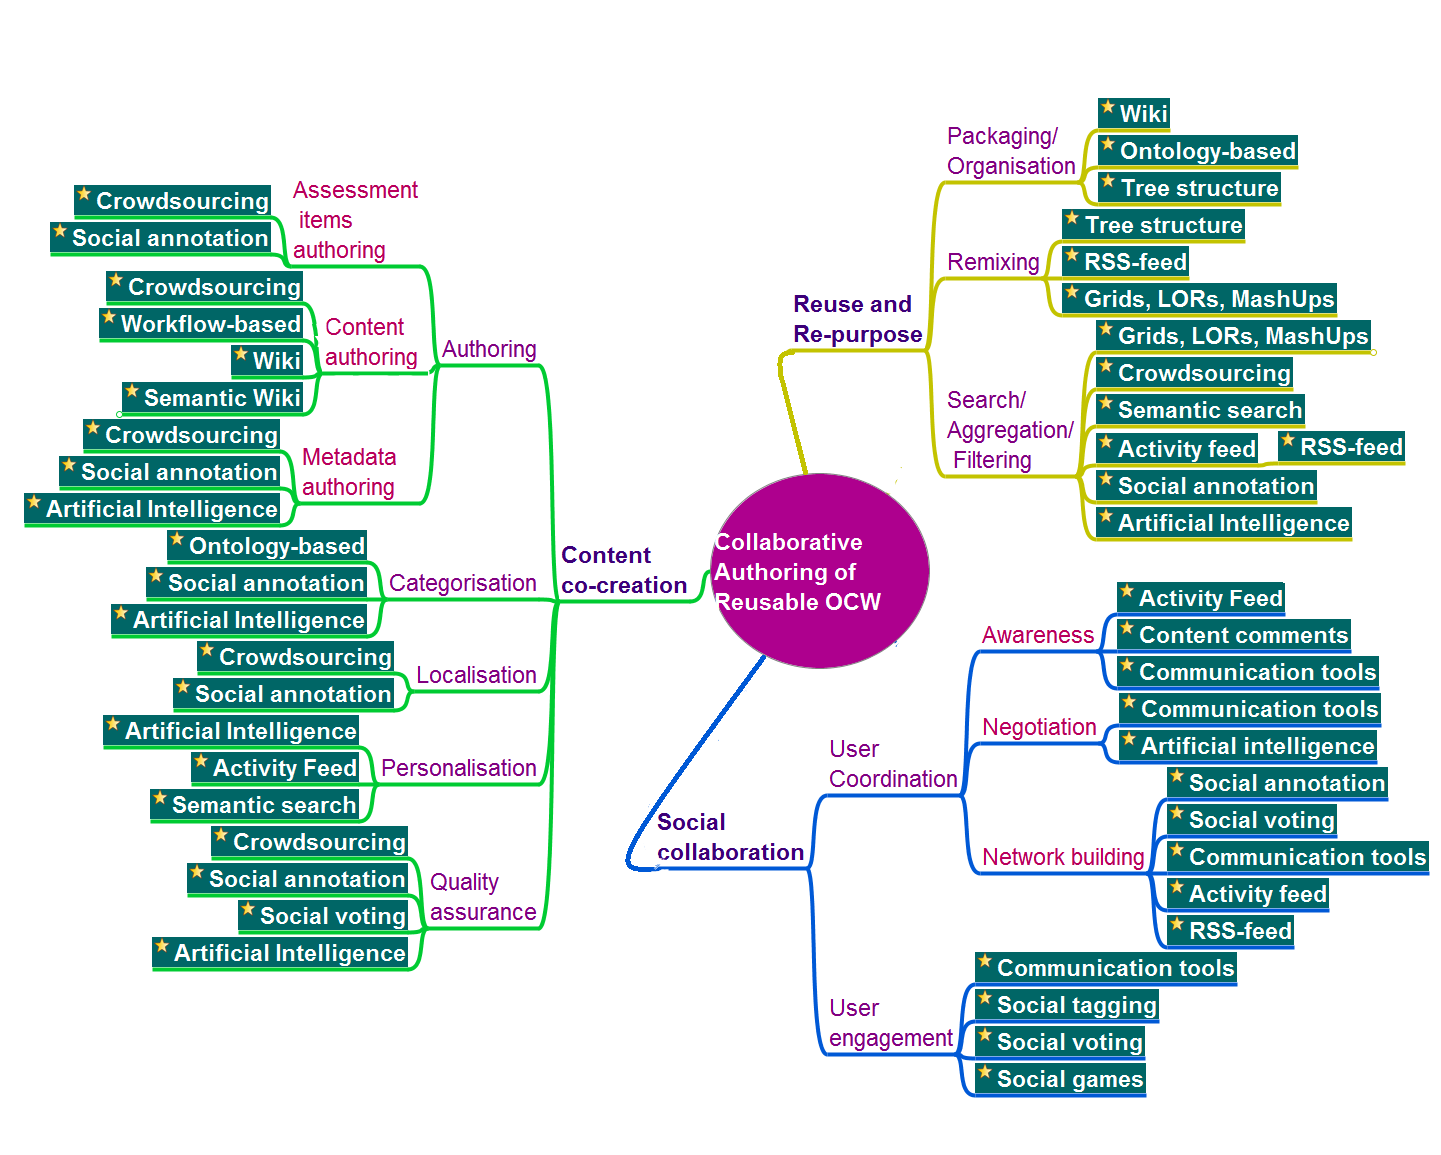
\includegraphics[width=\textwidth]{images/super_map.png}
  \caption{The mind map for Collaborative authoring of reusable OCW}
  \label{fig:super_map}
\end{figure*}

\section{Terminology}
\label{sec:Terminology}
During our study we faced plenty of ambiguous terms and domain-based concepts that might be unclear for non-education specialists, for example, computer scientists aiming to implement an approach.
In this section we focus on such terms, collecting their definitions and making our own conclusions on their appropriate usage.

\subsection{Learning}
\textbf{E-learning} - a learning conducted on the Internet~\cite{Dahlan2010}.
A wide set of applications and processes, which use available electronic media and tools
to deliver vocational education and training~\cite{de2009rss}.\\
\textbf{SMLearning} - type of e-learning that assumes the functions of a Social Media platform and extends its features to educational context~\cite{Claros2013}.\\
\textbf{Blended learning} - the (organic) integration of online digital learning and face to face classroom learning\cite{Cai2010}.\\
\textbf{Adaptive learning} - learning that enables learners to customize their learning environments and dynamically adapts learning content to learners' learning needs~\cite{brusilovsky2001adaptive}\\
\textbf{Virtual attendance} - the combination of synchronous and asynchronous ICT tools used to provide distance-education students with the same educational experience that conventional students receive in face-to-face (henceforth, F2F) taught classes.\\

\subsection{Content}
\textbf{Learning object} - a small, reusable digital component that can be selectively applied - alone or in combination - by computer software, learning facilitators or learners themselves, to meet individual needs for learning or performance support~\cite{shepherd2000objects}.
A later IEEE definition states: any entity digital or non-digital, which can be used, re-used, or referenced during technology-supported learning~\cite{learn_definition2002}.
In the context of Semantic Wikis \citeauthor{Li2010a} expands the term to include any real world objects such as people, places, organizations and events.\\
\textbf{Learning Object Repository (LOR)} - a general term for an online collection of learning objects.\\
\textbf{OCW} - a combination of learning objects, organized in a structured way according to predefined curriculum and serving as a unit for achieving a certain learning goal.\\
\textbf{Adaptive OCW} - OCW that is suitable to be used in adaptive learning environments.\\
\textbf{Curriculum} - structured plan that describes the educational program that is used in the educational resource~\cite{Marcilla2012}.\\
\textbf{Multimedia presentation} - a digital slide presentation which includes diverse media objects such as graphics and videos~\cite{Hong2012}.\\
\textbf{Learning Design (LD)} - a sequence of (collaborative) learning activities. It can incorporate single learner content, but also collaborative tasks such as discussion, voting, small group debate, etc. LD can be stored, re-used, customized, etc~\cite{Romero-Moreno2007}.\\

\subsection{Authoring}
\textbf{Cooperation} - a division of the labor among participants, into activities where each person is responsible for a portion of the problem.~\cite{roschelle1995construction}\\
\textbf{Collaboration} - a mutual engagement of participants in a coordinated effort to solve a problem together.~\cite{Romero-Moreno2007}\\ 
\textbf{Communities of practice} - the communities in which there exists “the sustained pursuit of shared enterprise~\cite{wenger1998communities}.\\
\textbf{The community-build system (CBS)} - a system for content creation by a community operating on a dedicated engine (e.g. Wiki)~\cite{Ro.zewski2011}. Also, it is a system of virtual collaborations organized to provide an open resource development environment within a given community. \\
\textbf{Wiki} - a Website that allows visitors to add, remove, edit and change content~\cite{Dahlan2010}. A collection of web pages designed to enable anyone who accesses it to contribute or modify content using a simplified markup language~\footnote{\url{http://wikipedia.com}}.
A web application which allows people to add, modify, or delete content in collaboration with others~\footnote{\url{http://en.wikipedia.org/wiki/Wiki}}.\\ 
\textbf{Semantic Wiki} - a wiki that enables simple and quick collaborative text editing over the Web and Semantic Web. Semantic wiki extends a classical wiki by integrating it with the management capabilities for the formal knowledge representations~\footnote{\url{https://goranzugic.wordpress.com/2010/09/09/semantic-wikis/}}.\\
\textbf{Collaborative authoring} - occurs in project like settings, where the project delegates authoring sub-tasks to a group of authors.
This kind of authoring needs synchronization, dialogue support, and coordination of the whole project~\cite{dicheva2002collaborative}.\\
\textbf{Cooperative authoring} - mainly involves synchronous re-usage of authoring products, such as course materials, libraries, ontologies, etc~\cite{dicheva2002collaborative}.\\ 
\textbf{Crowdsourcing} - a problem-solving approach that outsources tasks to an undefined, often anonymous, population~\cite{howe2006rise}. \\
\textbf{Workflow} - a sequence of industrial, administrative, or other processes through which a piece of work passes from initiation to completion.\\
\textbf{Workflow-based approach} - an approach that uses workflow for solving a task.\\
\textbf{Social annotation (Social tagging, folksonomy)} - a system of classification derived from the practice and method of collaboratively creating and translating tags to annotate and categorize content~\cite{peters2009folksonomies}.\\
\textbf{Awareness} - in the context of collaborative authoring, it is an understanding of activities of other collaborators, which provides a context for the own activity~\cite{Halimi2011}.\\
\textbf{Knowledge sharing} - an activity where agents - individuals, communities, or organizations - exchange their knowledge - information, skills, or expertise~\cite{ireson2010knowledge}.\\

\subsection{Technical Concepts and Technologies}
\textbf{Ontology} - a formal naming and definition of the types, properties, and interrelationships of the entities that really or fundamentally exist for a particular domain of discourse~\footnote{\url{http://en.wikipedia.org/wiki/Ontology_(information_science)}}.\\
\textbf{Activity feed (Activity stream)} - a list of recent activities performed by an individual(s), typically on a single website or on a single content piece.\\
\textbf{Mashup} - (in the domain of OCW authoring) it is a web page, or web application, that uses content from more than one source to create a single new learning object or OCW.\\
\textbf{RSS} - originally \emph{RDF Site Summary}, but often dubbed as \emph{Really Simple Syndication}.
It is a mechanism to publish a feed of frequently updated information: blog entries, news headlines, audio, video etc.\footnote{\url{http://en.wikipedia.org/wiki/RSS}}.\\
\textbf{RSS aggregator} - a tool that periodically checks for updates to the RSS feed and keeps the user informed of any changes~\cite{andersen2007web}.\\
\textbf{Grid} - a collection of independently owned and administered resources which have been joined together by a software and hardware infrastructure that interacts with the resources and the users of the resources to provide coordinated dynamic resource sharing in a dependable and consistent way according to policies that have been agreed to by all parties~\cite{hamid2010efficient}.\\
\textbf{Virtual Learning Environment (VLE)} - tools that support e-learning through integrated provision of learning materials, and communication, administration, and assessment tools~\cite{Currier2002}.\\


\section{Educational Content Co-creation Studies}
Changing reality poses new conditions and requirements for e-learning platforms.
As it is mentioned in~\cite{DBLP:reference/ai/PedreiraSC09}, ``\emph{the amount of knowledge that we deal with is much bigger than before, the interrelations between different forms of information are much more complex}''.
Due to this, new approaches for learning process organization have to be created.
Thus, a model in which a teacher is the monopolizing agent and the authorized representative of knowledge is no more adequate.
Learners should be allowed to have their own knowledge and share it with teachers, in other words teachers and learners should be able to switch their roles during the learning process.
The possibility of any user, including learners to edit the content together with modification history and discussion pages positively influences the reliability of the content.~\cite{Jiake2010}
In the section we summarize the known solutions and techniques to facilitate all aspects of such large-scale collaboration on open educational content.

\subsection{Collaborative Content Authoring}

During the literature study we have found three approaches of how the large-scale collaboration on educational content can be organized.
The first solution is to use a complex of (interconnected) web2.0 services.
For example, an approach described in \cite{Cai2010} proposes the combination of Google Site, Google groups, microblogging and RSS technologies to collaboratively create OCW for blended learning.
Course site includes curriculum, description, learning guide and teaching calendar.
The updates on the site are sent to all subscribers through RSS.
Site administrators can manually create a topic on the Google Groups page to discuss arguable changes before approving them.
The similar approach proposed in \cite{Bow2013} uses Google Drive to create self-assessment questions.
The produced questions are then converted into digital flashcard by self-developed freely distributed Java-based program.
The authors explain the choice of Google Drive by three factors: (1) Multiple people can simultaneously edit and view a document, spreadsheet, or PowerPoint, (2) it is user-friendly, and (3) just about all students are familiar with it.

The second solution is to add support of collaboration to existing non-collaborative OCW authoring tools.
In the approach~\cite{Greenhow2009} authors integrate Joomla, Moodle and MediaWiki to support the collaborative authoring of educational content.
The authors choose Joomla as the basis authoring tool due to the possibility to insert video records, Latex formulas, applets and highlighted code fragments.
Moreover, during the content creation process, a publicly available knowledge base for each course is created through collaborative content annotation.
The similar approach is described in \cite{hubscher2003constructive}.
The proposed web-based system allows students to share algorithmic representations with their peers.
Students can create their algorithmic representation using any utility or software, and can upload those files using the system.
These representations are then available for other students to view, evaluate and discuss through discussion forums.

However, we have concluded that the most popular and promising solution is to use an integrated platform based on wiki technology. 


%\todo{survey of wiki in education: \cite{Forte2007}}
%\todo{\url{http://books.google.de/books?id=HDKA8ViZcpsC}}
%\todo{Curriki, Wikiversity}
%\todo{survey: \cite{Nesic2010}}
%\todo{a survye: \cite{Chiribuca2008}}
%\todo{an approach, read: \cite{Nesic2008}}
%\todo{\cite{Pansanato2007}}


Through the study of existing literature (\cite{Jiake2010, Gokcearslan2011}),  the list of benefits of the wiki technology when applied to educational context includes:
\begin{itemize}
\item users (teachers and students) are able to contribute to their private collections of various learning resources (documents, files, photos, videos, software etc,.) by uploading to given positions
\item wiki-based collaborative learning environment provides a completely user-editable environment and thoroughly integrate the roles of author and reader.  
\item users can organize their resources in a thematic way, designing and creating different tags and share them with other users.
\item authoring a wiki on a given topic produces a linked network of resources.
\end{itemize}


However, the specific of wikis arises a number of issues when applied to OCW authoring. 
The technical issues are indicated, for example in \cite{wang2004extending, elrufaie2005wiki}:
\begin{itemize}
\item All content is modifiable by any user. The instructor may want to restrict modifiability of certain pages.
\item All content is open to everybody. A page, of which an important part is being developed, may be undesired to be issued, but wikis do not permit this.
\item Simultaneous edits are allowed, but not successful. When simultaneous writings are being performed on a page, wikis are locked.
\item Wikis can be evolved without end. An instructor may want to end the evaluation when the class ends; many wikis do not allow this.
\end{itemize}

Apart from the technical issues, there are two major obstacles preventing the usage of wikis in OCW development: (1) absence of possibility to structure the content as it is required by the learning object definition and (2) user engagement.


\subsection{Content Categorization}

The content categorization challenge is one of the key features of collaborative authoring systems.
This is due to the fact that it enables (semi-)automatic combination of learning objects into OCW, strongly improves the searchability of the learning artifacts and allows to implement more advanced content quality control techniques.
The conventional approach to content categorization is to choose one or more topics or concepts which the content piece is related to, usually from the pre-defined list.
However the approach lacks flexibility and requires a strong pre-development planning, that is not always possible when the content is developed through collaborative iterative process.

One solution is to allow building the predefined list of interconnected concepts in the same manner as the content pieces: through the large-scale collaboration.
In order to enrich such lists with the structure and semantic a number of authors propose to use ontologies.
Even more technologically advanced approach is to use the combination of social annotation techniques and artificial intelligence methods, allowing to (semi-)automatically cluster the content pieces based on the annotations.
And finally, the most advanced, and due to this the most functional, approach is to combine social annotation and collaboratively developed ontologies. 

This approach is implemented by a number of various authors \cite{Zhang2007, Agnew2010, Lee2010, Moro2011, Ghali2009, Achananuparp2007}, within which we consider the approach described in~\cite{Zhang2007} to be the most illustrative.
The proposed system works with code snippets, allowing users to annotate them.
Based on the annotations those content pieces are later added as individual learning objects to the courses based on the collaboratively developed curricula presented in a form of ontology.
The ontology underlying the curricula can be updated and edited by the users as any other content piece. 
The topic matching is done using methods of artificial intelligence, such as NLP and machine learning techniques, however it can be later changed manually by any user.
The byproduct of the approach is the ability to apply content recommendation and personalization approaches, as described in~\autoref{sec:content_personalization}

\subsection{Content Personalization and Recommendation}
\label{sec:content_personalization}

As it was discussed above, the content personalization and recommendation approaches are based on the content categorization.
Here by content recommendation systems we mean the ability of the platform to recommend to a learner a set of learning materials based on her background, interests or progress in other courses.
The content personalization (or adaptation) system goes one step further and after selecting a set of suitable material organizes it in a complete course.
Often the content personalization algorithms are able to adjust the initially provided course according to the learner performance.

In the scope of the thesis research we were not focused on the algorithms and approaches for the content recommendation and personalization.
Instead, we were interested in what steps should be done on a stage of content development in order to ensure that the content can be (re)used in systems supporting content recommendation and personalization features.
Based on the research done \cite{Brooks2006, Ghali2009, Cabada2011}, we consider that a list of annotations attached to each learning object in combination with fine-grained content structuring make the OCW suitable for use in those systems.



\subsection{Content Localization}

The content localization issue is one of the less-discussed issues in state-of-art research.
This is due to the fact, that the issue can not be effectively solved without solving related issues, such as community building, content structuring and synchronization, content quality assurance and other.

In the approach described in \cite{Leinonen2010} the authors implement the possibility to translate the content by collaborators.
Each new learning object created by the translation has its own metadata and can be further developed.
However, neither the possibility to update the translation if the original object was changed nor vice versa are implemented.
The synchronization is especially important, if versions in different languages are developed simultaneously, what often happens in open large-scale collaborative platforms.
In the scope of our research we provide our own solution to this issue (see ~\autoref{sec:multilinguality}).

\subsection{Content Quality Assurance}

Since the emergence of the OER movement, the quality of the open educational resources was a widely discussed issue.
A number of authors were working on defining and summarizing the key factors for the OER's quality.
For example, the following criteria are listed in ~\cite{travelwell, Leinonen2010}:
\begin{itemize}
\item They should be relevant to the learner and thus easily modified to fit the learner’s needs.
\item They should be of good quality and contain no factual errors.
\item They should disclose their point of view and in the case of science be free from bias.
\item They should not have hidden costs or prohibiting limitations on use.
\item A good learning resource should also be able to "travel well", to be easily translated and recontextualised
\end{itemize}

In \cite{sahar_vahdati_2015_14756} the authors formally define and discuss objective metrics which can be used for measuring an OER quality. 
They consider the following ten factors to determine the OER quality:
\begin{itemize}
\item Legal Reusability
\item Multilinguality
\item Format re-purposing
\item Recency
\item Sustainability
\item Availability
\item Learnability by Self-assessment
\item Learnability by Examples and Illustrations
\item Community Involvement
\item Discoverability
\end{itemize}

The list of factors correlates well with the challenges of the collaborative OCW authoring we defined. 
Thus, solving the challenges will guarantee high quality of the resulting OERs according to this list of factors.


\section{Educational Content Reuse and Re-purpose Studies}
\label{sec:state_of_art_reuse}

The importance of creating reusable and re-purposable e-learning objects is widely accepted by the e-learning community~\cite{Devedzic:2006:SWE:1177224}.
However, most of the works address the learning object reuse problem rather by means of semantic meta-data annotations, content tagging and packaging than by creating richly structured, reusable learning objects from the ground.
The importance of creating learning objects already with reuse in mind was, for example, stated by~\cite{DBLP:reference/ai/PedreiraSC09}: \emph{Content ... should be represented not as an object of study but rather as necessary elements towards a series of objectives that will be discovered in the course of various tests}.

%\subsection{Content Structuring}

There are only few approaches for the direct collaborative authoring of reusable content, such as, for example, learning examples creation~\cite{DBLP:conf/iadis/KuoTKHLC08} or semantic structuring and annotation of video fragments~\cite{DBLP:journals/ile/BarriocanalSAL11}.
This is due to the fact that the state-of-art collaborative authoring technologies do not deal with the (semi-)structured content.

As it was previously discussed in \autoref{sec:wiki}, conventional wiki technology has not been yet fully applied to the structured content development.
However, a couple of researches make steps in this direction.
Thus, \cite{DBLP:conf/wikis/HaakeLS05} introduces the concept of wiki templates that allow end-users to define the structure and appearance of a wiki page in order to facilitate the authoring of structured wiki pages.
Similarly the Hybrid Wiki approach~\cite{DBLP:conf/icsoft/MatthesNS11} aims to solve the problem of using (semi-)structured data in wikis by means of page attributes.

Another approach to combine wiki technology with structured representation are semantic wikis~\cite{DBLP:journals/software/SchaffertBBK08}.
Keeping the ability of traditional Wikis to collaborative content building, Semantic Wikis allow to add meaningful relationships between resources.
There are two types of semantic wikis.
Semantic text wikis, such as Semantic MediaWiki~\cite{smw:jws07} or KiWi~\cite{DBLP:conf/semwiki/SchaffertEGKRSS09} are based on semantic annotations of the textual content.
Semantic data wikis, such as OntoWiki~\cite{heino-n-2009-61-a}, are based on the RDF data model in the first place.
Both types of semantic wikis, however, suffer from two disadvantages.
Firstly, their \textit{performance and scalability} is restricted by current triple store technology, which is still an order of magnitude slower when compared with relational data management, which is regularly confirmed by SPARQL benchmarks such as BSBM~\cite{DBLP:journals/ijswis/BizerS09}.
Secondly, semantic wikis are generic tools, which are not particularly adapted for a certain domain thus substantially increase the usage complexity for users.
The latter problem was partially addressed by OntoWiki components such as Erfurt API, RDFauthor and Semantic Pingback, which evolved OntoWiki into a framework for Web Application development~\cite{heino-n-2009-61-a}.

%The list of benefits of using Semantic Wikis in OCW production according to \citeauthor{mu2012research, Rodriguez-Artacho2011, Li2010a}:
%\begin{itemize}
%\item Information or resources are co-built in the form of natural language, so more people can participate in the process in different roles, and contributor of resources is no longer confined to professional resource construction team, subject matter experts or knowledge engineers;
%\item The resource has formatted structure after annotated by ontology, which means based on the ontology annotated consistent structure, thus resources can be reused easily;
%\item Clear description of the relationship among information or resources can improve the effectiveness and comprehensiveness of navigation and retrieval;
%\item Collective participation of resources can solve the problems of the cost spent on the building and maintenance of open educational resources;
%\item From the aspect of OCW authoring these platforms allow to collaborate on the content and on course structure (or curriculum) at the same time.
%\item Lastly, the two processes of building and application are closely integrated together. User assumes dual roles as both user and contributor, which makes resources can meet user's requirement.
%\item the possibility to add dynamically created lists or tables to a page by using inline queries.
%This makes up-to-date query results available to readers who are not even aware of semantic queries.
%\end{itemize} 
%\todo{rephrase the list} 


We should also mention the \emph{Learning Objects Repositories} (LORs), that allow to produce structured reusable content.
The first of them, \emph{Connexions}~\footnote{\url{http://cnx.org/}}, presents the learning material as a combination of paragraphs, each of them could be easily edited or deleted.
However, this structuring is done more for comfortable editing and does not have any functional benefits: the paragraphs cannot be reused or annotated independently.
Thus, Connexions presents just an improved user interface for  wiki-based system.
The second example of structuring, is \emph{LeMill}~\footnote{\url{http://lemill.net/}}.
LeMill provides a way of collaborative editing of the presentations by implementing presentations as a group of images which can be edited collaboratively.
However, to edit a slide, a user has to replace it with another one.
Also, it is impossible to have several subgroups of the slides within a presentation.
The search through the slides (not presentations) is also not implemented.
Thus, slides cannot be manipulated as independent learning objects.


%The predecessor of Semantic Wiki is a CMS build on ontology.
%An example of such system developed for authoring OCW is \cite{dicheva2002collaborative}.
%
%
%\citeauthor{mu2012research} claims that semantically annotated knowledge not only improves the effectiveness of the information query and retrieval, but also improves the reusability of resources.
%
%\citeauthor{Li2010} define the following functionality of semantic wikis advantageous to conventional ones: (1) enhanced navigation and search possibility due to semantic annotations; (2) possibility to contextually adapt the presentation of the content; (3) better reusability due to flexible structure of the courses built from individual learning objects; (4) possibility to export the courses into other systems converting them in XML; (5) easily implemented activity recording. 
%All these features increase the usability of the course in compare with conventional wiki courses.
%\todo{prove?}




%\subsection{Content Remixing}
%\paragraph{Grid Portals}
%\cite{Shih2008}
%\cite{hamid2010efficient} addresses the problem of low performance by implementing OCW authoring platform using a Grid architecture.
%In their implementation a user navigates to the portal page, where the personalized list of appropriate applications that the user may interact with is presented.
%The list is build taken into account user identity and the authorization policies.
%The Grid Portal uses GridSphere to run the portal and Apache Tomcat to run the web-interface. 
%The authors consider the following list of benefits of Grid technology:
%\begin{itemize}
%\item Users are able to use his/her private workplace to invoke any application from a remote
%system
%\item Users are able to use the best suited system for executing their desired particular application, 
%\item Users are able to access data securely and consistently from remote sites, 
%\item Users are able to exploit multiple systems to complete complex tasks in design or authoring a courseware, 
%\item Users are able to use multiple systems to solve large problems that exceed the capacity
%of a single one. 
%\item The sharing does not mean simply exchange of data or files but rather a concrete access to resources which is especially important in synchronous collaborative design and authoring of a courseware.
%\end{itemize}
%
%Overview picture and description: \cite{Patricia2010}
%Study: \cite{Rosmala2012}
%\cite{Conole2010}
%\cite{Ghali2009}
%survey: \cite{Nesic2010}

%\subsection{Content Search and Filtering}
%Due to this the effectiveness and comprehensiveness of information retrieval increases~\cite{mu2012research}.
%Giving full play to the advantages of both Semantic Web and Wikis, Semantic Wiki supports social construction and development of constantly evolving and optimizing knowledge.
%Using Semantic Wiki, subject experts and knowledge engineers collaborate to build public ontologies in their field.
%These ontologies are then used to do semantic annotation to educational resources (including text, video, audio, etc.)



\section{Social Collaboration on Educational Content Studies}

In order to facilitate the social collaboration, two main features have to be enabled: user coordination and user engagement.
In the section we discuss requirements for the features' implementation found in the selected papers. 

\subsection{User Coordination}

One critical issue in collaborative authoring is the user coordination. 
In order the collaboration was efficient, all authors including novices must \emph{be aware} of the state of the production process, current goals and emergent issues.
State-of-art researchers~\cite{Nurjanah2011} distinguish following forms of user awareness: 

\begin{enumerate}
\item \emph{Personal awareness} relates to authors' knowledge of what they have done in the collaborative authoring process, allowing users to review their past work and plan future actions based on that.
\item \emph{Informal awareness} is related to the provision of information about who is in the collaborative work environment and what other authors have done during particular periods of time.
\item \emph{Group awareness} relates to authors's shared awareness of what has to be done.
\end{enumerate} 

To enable support of the \emph{personal awareness}, all user actions should be recorded and presented for example as user's activity feed in her profile.
The activity feed should summarize information about what a certain author has done, which objects she has created or updated, when it has happened. 
It should as well allow to go directly to the edited object.

To support \emph{informal awareness}, in addition to the personal activity feed, an object activity feed should summarize actions done to the object by all users.
As well, user comments on the process should be stored and attached to the object in order to prevent discussions over the same question twice. 
Therefore, (novice) authors can easily find all annotations and comments that relate to a particular object and know what other authors have been doing recently.

To support the \emph{group awareness}, some sort of an authoring plan should be available for all (prospective) collaborators.
The planning can be done explicitly in a form of a separate document attached to the content object.
As well, implicit planning can be chosen, when the scope of work is clear from the content structure. 
In case of implicit planning authors should be aware of empty and filled out (agreed) parts of the content, as well as about number of collaborators working on each part.



\subsection{User Engagement}
\label{sec:user_angagement}
The issue of user motivation raises from the fact that individuals contribution is encouraged by the certain collaborative authoring platform popularity~\cite{Bruckman2008}. 
This makes it difficult to motivate users to contribute within a newly developed platform.
Collaboration on projects like Wikipedia articles and open-source software is made easier by the fact that the goal is relatively well defined.
Thus, the solution is to turn the development of each content piece into a mini-project.
A number of authors define factors helping to proceed this turn and thus to increase authors participation ~\cite{Bruckman2008, foord2007stolen}: 

\begin{itemize}
\item Easy first step towards participation that is legitimate.
A newcomer should have something easy and satisfying to accomplish.
From this initial task, there are a series of gradually more challenging tasks available.
Users should be informed about what is expected to accomplish in each individual content piece and starting points for editing should be indicated.
\item Social support for participation and learning.
The presence of other collaborators who can potentially support her should be clear for a newcomer.
\item Clear major objectives, understood by all its users gives collaborators feeling of the 'collaborative ownership' of the content.
Working on a project the user cares about can motivate her to persevere when difficulties are encountered.
\item Users are highly motivated if there exist definitive times for different 'stages' of use and definite end point.
\item Clear indication of who can edit, which parts they can edit, acceptable and unacceptable use as well as clear navigation structure help users to feel confident while contributing.
\end{itemize}

Within other methods of user engagement the most promising are the ones based on gamification.
For example, digital badges, rewarding users for certain achievements, can be shown not only inside the platform, but as well in the user's profile pages in popular social networks.
This fact makes the successful work inside the platform more beneficial for a user, as she can use the badges earned for proving her skills for further online and offline projects. 




%\paragraph{Content Publishing}
%Initially, the content publishing issue lies outside the scope of our interest.
%However, the collaboratively created content must be published in efficient way, in order to collect a sufficient number of contributors from the crowd. 
%When speaking of efficient content publishing, we are meaning that the content should have high levels searchability and interoperability.
%Our approach proposes semantic publishing of the content, as described in ~\autoref{sec:RDB2RDF}.

%%==============================================================================
%\chapter{Reusable Educational Content}
%\label{chapter:reusability}
%%==============================================================================
%
%\epigraph{I liked the idea that a piece of information is really defined only by what it's related to, and how it's related. There really is little else to meaning. The structure is everything.}{Tim Berners-Lee}
%
%\section{Importance of Structuring}
%\label{sec:importance_of_structuring}
%
%\section{Educational Content Formats and Standards} 
%\label{sec:metadata}
%\subsection{Standards}
%
%\todo{LeMill: -tiny survey \cite{Leinonen2010}}
%
%
%
%\cite{Ola2009} studies open standards for e-learning.
%
%\cite{Rego2008} studies the standards and specifications for content structuring and annotation.
%Their compartment from aspect of supporting features is presented in \autoref{table:standards}.
%
%\begin{table}[!ht]
%
%\centering
%\rowcolors{1}{white}{LightGray}
%\begin{tabulary}{\columnwidth}{L|CCCC}
%
%\toprule
%\textbf{Features} & IMS & AICC & SCORM & DublinCore \\
%\midrule
%
%\textbf{Metadata} 				& \checkmark 	& 				& \checkmark  	& \checkmark\\
%\textbf{Learner Profile} 		& \checkmark 	& 				&  				& \\
%\textbf{Content Packaging} 		& \checkmark 	& \checkmark 	& \checkmark  	&  \\
%\textbf{Q\&T Interoperability} 	& \checkmark 	& 				&  				& \\
%\textbf{DR Interoperability} 	& \checkmark 	& 				&  				& \checkmark \\
%\textbf{Content structure} 		& \checkmark 	& \checkmark 	& \checkmark 	& \\
%\textbf{Content Communication}	&  				& \checkmark 	& \checkmark  	&  \\
%\textbf{Learning Design} 		& \checkmark 	& 				&  				&  \\
%\textbf{Accessibility} 			& \checkmark 	& 				&  				&  \\
%\textbf{XML Bindings} 			& \checkmark 	&  				& \checkmark  	& \checkmark \\
%\textbf{RDF Bindings} 			& \checkmark 	& 				&  				& \checkmark \\
%\textbf{Learner registration} 	& \checkmark 	& 				&  				&  \\
%
%\end{tabulary}
%\caption{Standards and specifications comparative analysis\cite{Rego2008}} 
%\label{table:standards} 
%\end{table}
%
%
%
%\begin{table*}[!ht]
%
%\centering
%\rowcolors{1}{white}{LightGray}
%\begin{tabulary}{\textwidth}{L|CCCC}
%
%\toprule
%\textbf{Field} & LOM & DublinCore & ISO / IEC 19788 & Adapted ISO / IEC 19788\cite{Marcilla2012}\\
%\midrule
%
%\textbf{Code} & & &  & x\\
%
%\textbf{Title} & & &  & x\\
%
%\textbf{Annotation} & & & x & x \\
%
%\textbf{Contributor} & & & x & x\\
%\textbf{Organization} & & & x &  \\
%\textbf{User language} & & & x & \\
%\textbf{Audience} & & & x & x \\
%\textbf{Educational method} & & & x &  \\
%\textbf{Curriculum} & & & x & x \\
%\textbf{Theme of curriculum} & & & x & x \\
%\textbf{User role} & & & x & x \\
%\textbf{Learning outcome} & & & x & x \\
%\textbf{Assessment} & & & x & x\\
%\textbf{Methodology} & & &  & x \\
%\textbf{Prior knowledge} & & &  & x \\
%\textbf{Indicators of resource} & & &  & x\\
%\textbf{Resources reused} & & &  & x\\
%\textbf{Improvements} & & &  & x\\
%\textbf{Acceptance rates} & & &  & x\\
%\textbf{Code} & & &  & \\
%\textbf{Code} & & &  & \\
%\textbf{Code} & & &  & \\
%\textbf{Code} & & &  & \\
%\textbf{Code} & & &  & \\
%
%
%
%\end{tabulary}
%\caption{Comparison between the metadata fields used in the proposed implementations} 
%\label{table:metadata} 
%\end{table*}
%
%\subsubsection{SCORM}
%\label{sec:SCORM}
%\cite{Guo2008} mentions that Sharable Content Objects (SCO) can hardly impart complex facts adequately, that makes it unable to support adaptability of the produced OCW.
%To overcome the limitation, authors propose to add a new extension to the specification of SCORM by utilizing state diagrams from UML 2.0 instead of SCORM-LSTD to describe the states and actions of training participants.
%The proposed LMS provides a learning process engine which behaves as a state machine while interpreting the sequencing and navigation rules.
%As  soon as a learning state transition is triggered by a trainee's action, a course resource update action will then be executed to match the trainee's state of learning.
%The assessment action will trigger a global update of trainee learning states.
%Whether all states of a trainee will be updated is determined by an assessment value and calculated according to either individual self-assessment, auto-assessment and peer-assessment, or a synthesized value.
%
%
%\subsubsection{SMIL} SMIL(Synchronized Multimedia Integration Language) is a XML based markup language by W3C recommendation to create multimedia presentations~\cite{bulterman2005synchronized}.
%SMIL allows synchronization of the contents of a PowerPoint presentation file and a video file so that the presentation shows slides and video on the same topic at any given time.
%By synchronizing multimedia elements such as text, images, video and audio SMIL provides an easy way for authors to collaborate on multimedia presentations.
%The SMIL files are logically divided into two sections: the layout section and the body section.
%\citeauthor{Cheong2002} proposes to divide the files physically, allowing course designers to work on the template and on the content separately.
%As well, several templates can be assigned to the same course and users are able to switch between them on fly.
%By allowing users to do so, an approach address the issue of course accessibility for learners with special needs or low bandwidth (partially hiding less important elements and decreasing the complexity of interface design).
%An approach proposed in \cite{Hong2012} uses SMIL and collaboratively added annotations to turn the educational video files into rich learning resources.
%The uniqueness about this e-learning system is the connection between synchronized multimedia presentation authoring and real-time slide annotation.
%
%\citeauthor{Claros2013} combines SMIL technology and Social networking.
%The proposed approach uses Facebook API to manage users, notifications and groups.
%Youtube API is used to search video files and their metadata.
%In their approach multimedia content is combined out of video files, texts, images and questionnaires. 
%The questionnaires are added to video records by extending SMIL with \emph{question[id, open, region, type, title, label, feedback, optional]} and \emph{option} tags. 
%The sequencing of the learning objects can be done collaboratively, supported by discussion forums.
%The distinguishing feature of the approach is a versions management with a possibility to revert the changes.
%
%\cite{Tellez2008} - why SMIL is better, good overview and comparison with other standards
%
%\subsubsection{LRMI}
%Synergistic efforts of the Learning Resource Metadata Initiative (LRMI)~\footnote{\url{www.lrmi.net}}, funded by the Bill and Melinda Gates Foundation, establish a simplifi ed set of standards to tag all educational online content, making it easier to publish, discover, and deliver quality OERs on the Web.
%
%\subsubsection{RDF}
%RDF is an XML-based language for describing information contained in a Web resource.
%This Web resource can be anything, for example a Web page or a Website.
%RDF is the basic building block for supporting the Semantic Web, and is same as HTML is for the conventional Web.
%
%The properties of RDF are:
%\begin{itemize}
%\item RDF is a language recommended by W3C~\footnote{\url{http://www.w3.org/RDF/}} and it is all about metadata,
%\item RDF is capable of describing any fact (resource) independent of any domain,
%\item RDF provides a basis for \emph{coding}, \emph{exchanging}, and \emph{reusing} structured metadata,
%\item RDF is structured; i.e. it is machine-understandable. Machines can do useful operations with the knowledge expressed in RDF,
%\item RDF allows \emph{interoperability} among applications exchanging \emph{machine understandable} information on the Web.
%\end{itemize}
%
%Serializing RDF data is a crucial issue since different platforms and environments work better with different data formats.
%There are already several formats such as \emph{RDF/XML}, \emph{Turtle}, \emph{N-Triples}, \emph{Notation3}, \emph{N-Quads} and \emph{JSON-LD} for serializing RDF data.
%There are also formats such as \emph{RDFa} and \emph{Microdata} to embed RDF data within HTML documents by offering additional HTML attributes.
%
%\todo{RDF is from Ali's thesis}
%
%
%\subsubsection{RSS}
%RSS is a family of Web feed formats used to publish frequently updated content such as blog entries, news headlines, or podcasts.
%An RSS document, which is called a ‘‘feed,” ‘‘Web feed,” or ‘‘channel,” contains either a summary of content from an associated Web site or the full text.
%RSS makes it possible for people to keep up with their favorite Web sites in an automated manner rather than checking them manually.
%RSS content can be read using a software tool called ‘‘RSS reader,” ‘‘feed reader” or ‘‘aggregator.”
%A user subscribes to a feed by entering the feed's link into the reader or by clicking an RSS icon in a browser that
%initiates the subscription process.
%The reader checks the user’s subscribed feeds regularly for new content, downloading any updates that it finds.
%The proposed system translates each book into a RSS feed to help learners aggregate and read their learning materials
%in RSS readers.
%
%
%\section{Efficient Content Publishing}
%\label{sec:publishing}
%
%\

\section{Conclusions}

We have built our state-of-art study around four major research questions:
\begin{enumerate}

\item \emph{What are the main challenging tasks in collaborative authoring of reusable OCW?}
\item \emph{Which technologies are being used to solve these tasks?}
\item \emph{How well covered are the challenging tasks in the scientific literature?}
\item \emph{What are the main gaps in state-of-art research?}

\end{enumerate}


We have answered the first question by researching existing surveys.
According to our study, the main challenging tasks of collaborative authoring of OCW can be divided in three dimensions: (1)content co-creation, including metadata and assessment items authoring, classification, localization, personalization and quality assurance; (2) content reuse and re-purpose, including content organization, remixing, search, aggregation and filtering; (3) social collaboration, including user coordination and user engagement.

The technologies which are currently commonly being used for solving the tasks are Web 2.0, artificial intelligence and Semantic Web technologies.
We summarize the answers for these two questions in mind map presented in \autoref{fig:super_map}.

Having analyzed the paper distribution, we came to a conclusion that the issues and technologies of OCW collaborative authoring are covered in the literature with not enough depth, that means there is not enough \emph{detailed} and \emph{focused} studies on specific aspects and technologies.

The matrix we have filled out (cf. \autoref{tab:matrix}) gives additional details on the most and the least researched topics in the area.
Especially, we consider the following topics not to be sufficiently addressed: 

\paragraph{Content localization issue}
Although it is believed that the most important benefits OpenCourseWare would bring to the developing countries, the translation and localization approaches are almost ignored in the published research.
This gap is from one perspective is well-known, but from another perspective it is hard to solve.
The power of crowdsourcing can be used to translate the content with reasonable quality, but this rises the problems of content synchronization and cultural barriers.
The content synchronization is partly addressed by our proposed concepts (see \autoref{sec:multilinguality}), while the actual localization which considers the cultural differences and barriers still needs to be additionally researched. 

\paragraph{Content remixing}
The issue of content remixing is also often ignored in the state-of-art research.
The educational content has to be re-designed from year to year, new topics often should be included, as well as parts of different courses often need to be combined.
Although several approaches exist to address the challenge using mash-ups and LORs, these solutions do not involve content versionning and crowdsourcing. 
For example, an interesting approach proposed in~\cite{Auinger2009} uses RSS-feed and machine-learning algorithms for filtering the content from the feed and assembling it accordingly the user preferences.
A mash-up created in this way can be further edited by collaborators.
In ~\autoref{sec:wikiapp} we propose our own approach, assuming the content is authored in a wiki-way, has a tree-structure and due to that can be easily re-mixed.
An important novelty here is the comprehensive algorithm for versionning the content in a tree-structure.

\paragraph{Network building and User engagement}
These two aspects are interconnected and are important for the success of any collaborative systems.
Although several approaches are available from technological side (like digital badges or social gaming), only few approaches implement and evaluate them.
These aspects lack especially the evaluation and comparison of the existing methods. 
In our approach, discussed in details in \autoref{sec:Crowdlearn}, we propose to use social networking functions to build highly-connected user groups, sharing the ownership of the content.
As well, when developing the concept, we took into consideration the recommendations summarized in \autoref{sec:user_angagement}.

%==============================================================================
\chapter{Collaboration on Multilingual Structured Educational Content}
\label{chapter:collaboration}
%==============================================================================

\epigraph{The original idea of the web was that it should be a collaborative space where you can communicate through sharing information.}{Tim Berners-Lee}

\epigraph{I think in general it's clear that most bad things come from misunderstanding(...)}{Tim Berners-Lee}

While nowadays there is a plethora of Learning Content Management Systems (LCMS), the collaborative, community-based creation of rich e-learning content is still not sufficiently well supported.

When speaking about collaborative authoring, the crowdsourcing techniques and wiki paradigm are proven to be an effective solution, allowing continuous iterative increasing of the content quality while keeping the costs moderately low.
Such techniques suppose the collaborative platform supports content versionning, branching and merging, that prevents unwanted changes while allows uncontrolled list of collaborators to contribute.
The \emph{wiki} paradigm allows every user to refine the published content by facilitating small changes and providing easy-to-use markup language.
The best known example of successful crowdsourcing platform is Github, however there are adaptations of the crowdsourcing techniques to the domains other than classical software development, such as Wikipedia or OpenStreetMaps.
%The main obstacle for the adapting the crowdsourcing to the educational domain is the content presentation in (semi-)structured form.

However, the application of the crowdsourcing techniques to the OCW production has not yet been done.
This is due to the specific of the content type the concepts have to deal with.
The paradigm of \emph{Open Educational Resources} supposes the creation and sharing of reusable, re-purposable learning objects, annotated by standardized metadata.
Thus, the content structuring is required, as discussed in ~\autoref{sec:content_reusability_structuring}.
However, dealing with the structure when applying crowdsourcing techniques is challenging.

In the current chapter we present and discuss our \emph{CrowdLearn concept}, aiming at application of crowdsourcing techniques to the structured content and supportive \emph{WikiApp} data model we have developed to implement it.
As well, we present the CoSMEC concept, which enables the support of multilingual content for this complex data model.


\section{CrowdLearn Concept}
\label{sec:Crowdlearn}

In order to develop the concept which facilitates large-scale collaboration on OERs, we have first summarized the major challenges and possible solutions for that.
The results of this work have been already discussed in the previous chapter.
We have transformed the findings from our related work study in a \autoref{tab:chosen_app}, which gives a brief overview on the challenges and approaches we have found to be the most promising. 

\begin{table}[!ht]\scriptsize
\begin{tabulary}{1\columnwidth}{l|p{20em}|p{17em}}

\toprule
\textbf{Aspect} & \textbf{Approach chosen} & \textbf{Remarks} \\

\midrule

\rowcolor{LightGray}
\multicolumn{3}{l}{Content co-creation}\\
Content authoring & Crowdsourcing, wiki & \multirow{3}{17em}{Content objects, metadata, assessment items and styles are reusable and fully versioned}\\
Metadata authoring & Crowdsourcing, wiki, standard compliance \\
Assessmnt. items auth. & Crowdsourcing, wiki \\
Quality assurance & Social networking, crowdsourcing, wiki, semantic structuring & Synergistic effect  \\
Categorization & Crowdsourcing (social annotation) & \\
Personalization & Semantic structuring, crowdsourcing (social annotation) & \\
Localization & Crowdsourcing, wiki & Using CoSMEC concept. See \autoref{sec:multilinguality} for more details \\

\rowcolor{LightGray}
\multicolumn{3}{l}{Reuse and re-purpose}\\

Search, filtering, aggregation. & Standard compliance, crowdsourcing (social annotation), semantic structuring & \\
Remixing & Semantic structuring, standard compliance & Using WikiApp data model. See \autoref{sec:wikiapp} for more details \\
Organization & Semantic structuring & Using WikiApp data model. See \autoref{sec:wikiapp} for more details\\

\rowcolor{LightGray}
\multicolumn{3}{l}{Social Collaboration}\\
Negotiation & Social Networking & \\
Awareness & Social Networking & \\
Network building & Social Networking & \\
Engagement & Social Networking & \\


\bottomrule

\end{tabulary}
\caption{Chosen approaches for solving OCW collaborative authoring challenges}
\label{tab:chosen_app}
\end{table} 

\begin{figure}[tb]
\centering
	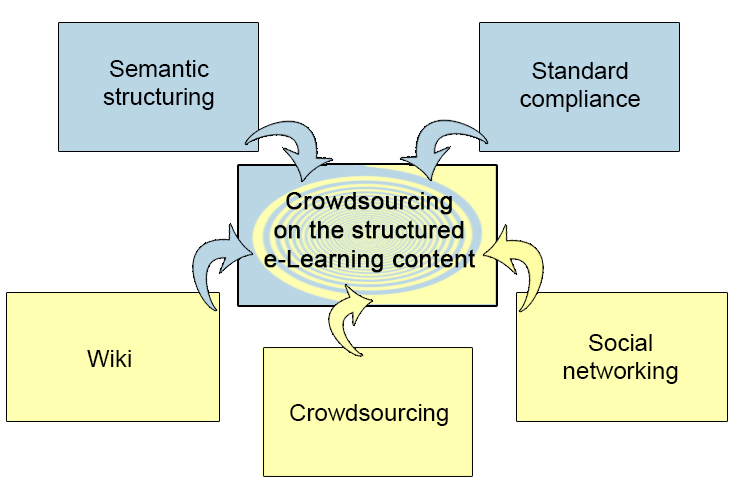
\includegraphics[width=0.75\columnwidth]{images/crowdlearn_updated.jpg}
	\caption{CrowdLearn concept.}
	\label{fig:conceptual_scheme}
\end{figure}

As it can be seen from the table, most of the challenging tasks can be covered by five strategical approaches, as illustrated by~\autoref{fig:conceptual_scheme} 
Moreover, the combination of the approaches gives a synergistic effect.
However, the integration of the approaches requires additional concepts to be developed.
We have called the resulting complex solution \emph{CrowdLearn concept}.
In the section we discuss the Crowdlearn concept and the synergistic effects it gives, while missing approaches we had to develop are discussed in the next sections.

The Crowdlearn concept aims to provide a framework for efficient collaborative authoring of reusable educational content.
We see the CrowdLearn concept as an application of crowdsourcing techniques to the e-learning content creation, re-purpose and reuse.
The sources of our inspiration were:
\begin{itemize}
\item Wiki paradigm and its implementation Wikipedia, the project which proved the effectiveness of applying crowdsourcing techniques to the textual content 
\item Content versionning systems and their online implementations (e.g. Github), which proved the reliability and effectiveness of opening large-scale projects for crowdsourcing with uncontrolled auditory. 
\end{itemize}
In order the application to be effective, the concept considers the specific of the educational domain by combining five strategies, presented in \autoref{fig:conceptual_scheme}.
Below we discuss the five main components and their interrelations.

\paragraph{Crowdsourcing}

There are already vast amounts of amateur and expert users which are collaborating and contributing on the Social Web.
Harnessing the power of such crowds can significantly enhance and widen the distribution of e-learning content.
Crowd-sourcing as a distributed problem-solving and production model is defined to address this aspect of collective intelligence~\cite{Howe2006}.
CrowdLearn as its main innovation combines the crowd-sourcing techniques with the creation of highly-structured e-learning content.
E-learning material when combined with crowd-sourcing and collaborative social approaches can help to cultivate innovation by collecting and expressing (contradicting) individual's ideas.
As Paulo Freire wrote in his 1968 book \emph{Pedagogy of the Oppressed}, `Education must begin with the solution of the teacher-student contradiction, by reconciling the poles of the contradiction so that both are simultaneously teachers and students...'.
Therefore, crowd-sourcing in the domain of educational material not only increases the amount of e-learning content but also improves the quality of the content.
Our concept assumes application of crowdsourcing techniques to all kinds of the content and its metadata, including self-assessment items.
This, together with social networking and semantic structuring, completely solves the challenges from the \emph{content co-creation} aspect group.
The content quality assurance is then reached through facilitation of small contributions from the crowd and ability to discuss the individual learning artifacts, such as an individual slide or a question.
Social annotation of the content pieces serves as a basis for content categorization and customization.
An important task our concept allows to be done by the crowd is content localization.
Here the content structuring plays a crucial role in improving the quality of the translation, due to the possibility to translate and edit each learning artifact individually.


\paragraph{Wiki}

The wiki paradigm supposes the crowdsourcing of the content supported by facilitation of small contributions, formatting and version control.
To be able to deal with structured content, the wiki paradigm needs a more comprehensive data model.
Our CrowdLearn concept assumes the content to be presented according to our previously developed WikiApp data model, described in details in ~\autoref{sec:wikiapp}.
The WikiApp data model is a refinement of the traditional entity-relationship data model.
It adds some additional formalisms in order to make users as well as ownership, part-of and based-on relationships first-class citizens of the data model.
A set of content objects connected by \emph{part-of} relations can be arranged and manipulated in exactly the same manner, as an individual non-structured object.
The model natively supports versioning and structuring of the different content objects.

\paragraph{Semantic structuring}

Instead of dealing with large learning objects (often whole presentations or tests), we decompose them into fine-grained learning artifacts.
Thus, rather than a large presentation, user will be able to edit, discuss and reuse individual slides; instead of a whole test she/he will be able to work on the level of individual questions.
This concept efficiently facilitates the reuse and re-purpose of the learning objects.
Semantic structuring facilitates application of content personalization mechanisms, allowing recommendation systems to work with a finer tuned setup.
Semantic structuring together with standard compliance and social annotation facilitates content publishing, aggregation and filtering due to the ability of algorithms to work with finer grained content.
The semantic structuring of the content is implemented via using WikiApp data model discussed in the paragraph above.

\paragraph{Social networking}

The theoretical foundations for e-Learning 2.0 are drawn from social constructivism~\cite{Wang2012}.
It is assumed that students learn as they work together to understand their experiences and create meaning.
In this view, teachers are knowers who craft a curriculum to support a self-directed, collaborative search and discussion for meanings.
Supporting social networking activities in CrowdLearn enables students to proactively interact with each other to acquire knowledge.
With the CrowdLearn concept we address the following social networking activities: 

\begin{itemize}
\item Users can follow individual learning objects as well as other users activities to receive notification messages about their updates. 
\item Users can discuss the content of learning objects in a forum-like manner. 
\item Users can share the learning objects within their social network websites such as Facebook, Google Plus, LinkedIn, etc. 
\item Users can rate the available questions in terms of their difficulty.
\end{itemize}

Besides increasing of the learning process quality, social activities improve the quality of the created learning material.
Even when answering a quiz, users can contribute by analyzing the quality of the questions and making suggestions of how to improve them.
Thus, the knowledge is being created not only explicitly by contributors, but also implicitly through discussions, answering the questions of assessment tests, or in other words through native learning activities.

\paragraph{Standard-compliance}
In order the CrowdLearn concept to be efficient in the real life, it has to support the content migration between different Learning Management Systems.
However, often content migration is not completely adequate and can thus result in loss of valuable content, metadata or structure.
Even if the transfer is possible, moving the content between systems can be more costly than just redeveloping that course in the new system.

The first possible strategy to overcome this challenge is the standard-compliance of both LMS and content.
During our research on the available content and metadata formats we have decided to adopt the \emph{SCORM standard}~\cite{scorm_specification2011} and practical recommendations~\cite{scorm2011}, expanding the standard to support the collaborative model of content creation (see \autoref{sec:SCORM}).
The other strategy is to use an intermediary format to proceed the migration.
For example, Linked Data is proven to perform well in the educational domain~\cite{guy2014linkedup}.  
We present our Linked Data model in~\autoref{sec:data_model_rdf}, and in~\autoref{sec:RDB2RDF} we describe the process of content transformation into RDF triples in detail.



\section{WikiApp Data Model}
\label{sec:wikiapp}
The implementation of the CrowdLearn concept requires a data model, that naturally supports required operations. 
However, to our knowledge, such model is not known to be described formulated at least in the open scientific research.
To fulfill the gap we have developed and formalize an innovative data model called WikiApp.

The WikiApp data model is a refinement of the traditional entity-relationship data model.
It adds some additional formalisms in order to make users as well as ownership, part-of and based-on relationships first-class citizens of the data model.
A set of content objects connected by \emph{part-of} relations can be arranged and manipulated in exactly the same manner, as an individual non-structured object.
The model natively supports versioning and structuring of the different content objects.

\begin{figure*}[htb]
	\centering
		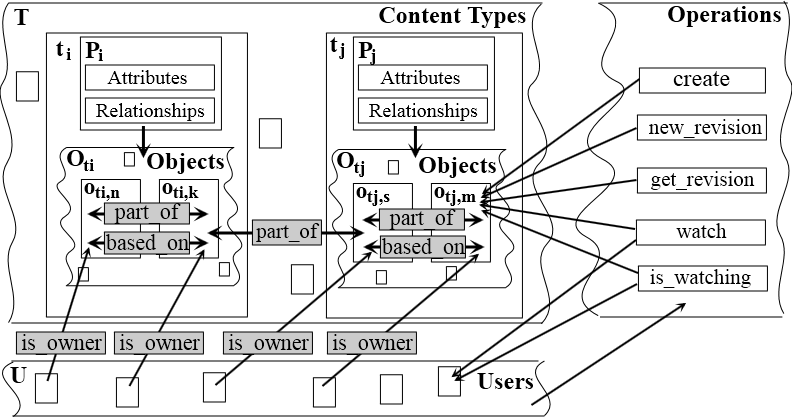
\includegraphics[width=\columnwidth]{images/data_model_last.png}
	\caption{Conceptual view of the WikiApp data model.}
	\label{fig:data-model}
\end{figure*}

We illustrate the WikiApp model in \autoref{fig:data-model} and formally define it as follows:

\begin{definition}[WikiApp data model]
\label{def:dm}
The WikiApp data model $\mathcal{WA}$ can be formally described by a triple $\mathcal{M}=(U,T,O)$ with:
\begin{itemize}
	\item $U$ - a set of \emph{users}.
	\item $T$ - a set of \emph{content types} with associated property types $P_t$ having this content type as their domain.
	\item $O=\{O_{t \in T}\}$ with $O_t$ being \emph{sets of content objects} for each content type $t \in T$.
\end{itemize}
	Each $O_t$ consists of content objects $o_{t,i}$ with $i \in I_T$ being a suitable \emph{identifier} set for the content objects in $O_t$.
	Each $o_{t,i}$ comprises a set of properties $P_{t,i} = Attr_{t,i} \cup Rel_{t,i}$.
	$Attr_{t,i}$ is a set of literal, possibly typed \emph{attributes}, and $Rel_{t,i}$ is a set of \emph{relationships} with other content objects;
	The only necessary attribute for all content objects is $c_{t,i}$, which contains the creation timestamp of the object $o_{t,i}$.
	$Rel_{t,i}$ can particularly include the following designated relationships to related objects:
	\begin{itemize}
		\item $part_{t,i} \subset O$ refers to \emph{set of the content objects} contained in $o_{t,i}$ ;
		\item $base_{t,i} \in O_t$ refers to \emph{base content object} from which the object $o_{t,i}$ was derived;
		\item $user_{t,i} \in U$ refers to a user being the \emph{owner} of the $o_{t,i}$;		
	\end{itemize}
\end{definition}

The WikiApp model assumes that all content objects are versioned using the timestamp $c_{t,i}$ and the base content object relation $b_{t,i}$.
In the spirit of the wiki paradigm, there is no deletion or updating of existing, versioned content objects.
Instead new revisions of the content objects are created and linked to their base objects via the \textit{base-content-object} relation.
All operations have to be performed by a specific user and the newly created content objects will have this user being associated as their owner.
In practice, however, usually only a subset of the content objects are required to be versioned.
For auxiliary content (such as user profiles, preferences etc.) it is usually sufficient to omit a base content object relation.
For reasons of simplicity of the presentation and space restrictions we have omitted a separate consideration of such content here.
However, this is in fact just a special case of our general model, where the base content object relation $base_{t,i}$ is empty for a subset of the content objects.

The model is compatible with \emph{both} the relational data model and the \emph{Resource Description Framework} (RDF) data model (i.e. it is straightforward to map it to each one of these).
When implemented as a relational data, content types correspond to tables and content objects to rows in these tables.
Functional attributes and relationships as well as the \textit{owner} and \textit{base-content-object} relationships can be modeled as columns (the latter three representing foreign-key relationships) in these tables.
%TODO add a link to RDF description
The implementation of the WikiApp model in RDF is slightly more straightforward: content types resemble classes and content objects instances of these classes.
Attributes and relationships can be attached to the classes via \verb|rdfs:domain| and \verb|rdfs:range| definitions and directly used as properties of the respective instances.
For reasons of scalability we expect the WikiApp data model to be mainly used with relational backends.

\textit{Watching} the users, as well as \textit{following} the learning objects operations are natively supported by the model.
This allows users to receive the information about changes of the followed content object or new objects created by the watched user.
Also, these operations allow to easily find the followed object or user.

\begin{example}[SlideWiki data model] 
\label{exa:sw}
For our Slide\-Wiki example application (whose implementation is explained in detail in \autoref{chapter:implementation}) the data model consists of individual slides (consisting mainly of HTML snippets and some meta-data), decks (being ordered sequences of slides and sub-decks), media assets (which are used within slides) as well as themes (which are associated as default styles with decks and users):
\begin{itemize}
	\item $T=\{deck,slide,media,theme\}$
	\item $Attr_{deck}=\{title \rightarrow text, abstract \rightarrow text,\\
		\verb|   |license \rightarrow \{CC-BY, CC-BY-SA\}\}$,\\
		$Rel_{deck}=\{default\_theme \rightarrow theme\}$,\\
		$Part_{deck}=\{deck\_content \rightarrow deck \cup slide\}$
	\item $Attr_{slide}=\{content \rightarrow text, speaker\_note \rightarrow text,\\
		\verb|   |license \rightarrow \{CC-BY, CC-BY-SA\}\}$,\\
		$Rel_{slide}=\{uses \rightarrow media\}$, $Part_{slide}=\{\}$
	\item $Attr_{media}=\{type \rightarrow \{image, video, audio\}, uri \rightarrow \\
		\verb|   |string, license \rightarrow \{CC-BY, CC-BY-SA\}\}$,\\
		$Rel_{media}=\{\}$, $Part_{media}=\{\}$
	\item $Attr_{theme}=\{title \rightarrow string, css\_definition \rightarrow text\}$,\\
		$Rel_{theme}=\{\}$, $Part_{theme}=\{\}$
\end{itemize}
\end{example}

After we introduced the WikiApp data model, we now describe the main operations on the data model.
In the spirit of the Wiki paradigm, there is no deletion or updating of existing, versioned content objects.
Instead new revisions of content objects are created and linked to their base objects via the $b_{t,i}$ relation.

\begin{definition}[WikiApp operations]
\label{def:operations}
Five base operations are defined on the WikiApp data model:
\begin{itemize}
	\item $create(u,t,p):U \times T \times P_t \rightarrow O_t$ creates a new content object of type $t$ with the owner $u$ and properties $p$.
	\item $newRevision(u,t,i,p):U \times T \times I_T \times P_t \rightarrow O_t$ creates a copy of an existing content object $o_{t,i}$ of type $t$ potentially with a new owner $u$ and overriding existing properties with $p$.
	\item $getRevision(t,i):T \times I_T \rightarrow O_t \cup {false}$ returns the existing content object $o_{t,i}$ of type $t$ including all its properties or false in case a content object of type $t$ with identifier $i$ does not exist.
	\item $isWatching(u,t,i):U \times T \times I_T \rightarrow \{true,false\}$ returns true if the user $u$ is watching the content object of type $t$ with identifier $i$ or false otherwise.
	Following users is a special case, where the content object type is set to user.
	\item $watch(u,t,i):U \times T \times I_T \rightarrow \{true,false\}$ toggles user $u$ watching the content object of type $t$ with identifier $i$ and returns the new watch status.
\end{itemize}
\end{definition}

All operations have to be performed by a specific user and the newly created content objects will have this user being associated as their owner.
In addition, when a new revision of an existing content object is created and the original content object is indicated to be part of another content object (by the distinguished part-of relations) the creation of a new revision of the containing content object has to be triggered as well.
In our Example~\autoref{exa:sw}, this is, for example, triggered when a user creates a new revision of a slide being part of a deck.
If the user is not the owner of the containing deck, a new deck revision is automatically created, so as to not implicitly modify other users' decks (cf. \autoref{sec:content_development_implementation}).

%\section{Social Aspects of Collaboration}
%\subsection{User motivation: gamification with digital badges}
%

\section{Co-evolution of Structured Multilingual Educational Content (CoSMEC)}
\label{sec:multilinguality}
In order to enable the support of multilingual educational content we have expanded the CrowdLearn concept to support multilinguality.
The proposed CoSMEC concept combines and expands several existing paradigms.
The overview of the concept is presented in~\autoref{fig:cosmec_concept}.

\begin{figure*}[!h]
\centering
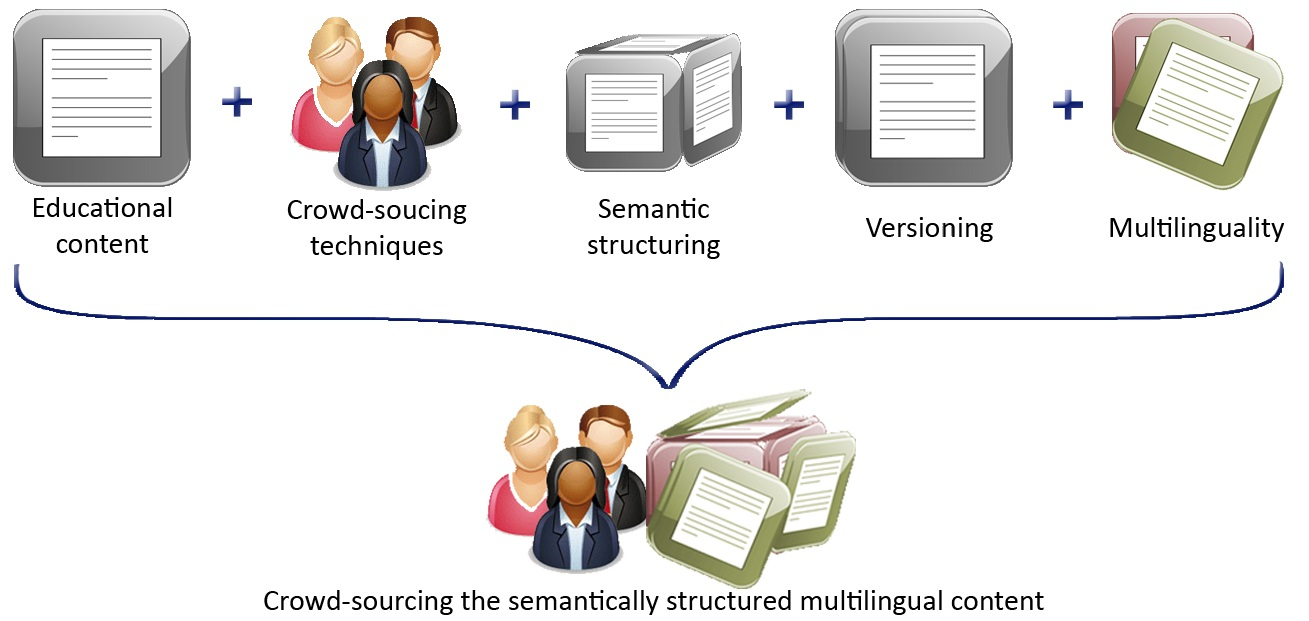
\includegraphics[width=1\textwidth]{images/CoSMEC_concept.jpg}\\
\caption{Overview of the CoSMEC concept}
\label{fig:cosmec_concept}
\end{figure*}

To enable collaborative authoring of semantically structured educational content, we use our CrowdLearn concept, as described in detail in~\autoref{chapter:collaboration}.
In order to enable the support of multilingual content, CoSMEC allows the content versions to be presented in different languages by adding the \emph{translatedInto} and its inverse \emph{translatedFrom} relations to the WikiApp data model.
CoSMEC does not deal with the objects being originally created in different languages.
Instead, our concept requires the presence of the \emph{source} content object, as well as its \emph{translations}.
Enforcing this requirement allows us to:
\begin{itemize}
\item distinguish between users' authoring and translating contributions to the content,
\item present the list of original content authors in all translations,
\item propagate changes in order to synchronize the content of translations with the source.
\end{itemize}  

The CoSMEC concept introduces the paradigm of \emph{co-evolution} of multilingual content, that means the ability to update a translation to the current state of the source object and vice versa.
However, the requirement above only allows users to update the content of a translation according to an original version, but not contrariwise.
To overcome this limitation, we enable the translation of an object back to the original language, thus creating a revision of the source object.
This \emph{back-translation} requires a mechanism of merging the revisions, as we do not want to overwrite the original content with a repeatedly-translated one.
Thus, in order to function efficiently, the mechanism of \emph{co-evolution} requires three operations to be defined:
\begin{itemize}
\item initial translation (see~\autoref{fig:double}, schema 1);
\item synchronization of the translation with the source (see~\autoref{fig:double}, schema 2);
\item merging the revisions (see~\autoref{fig:double}, schema 3)
\end{itemize}

\begin{figure}[!ht]
	\centering
		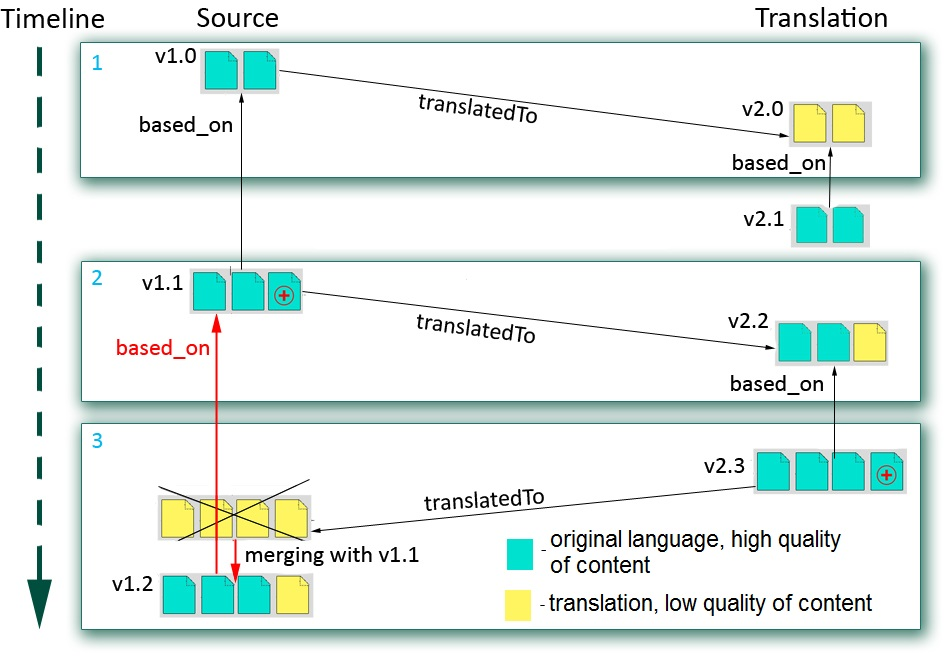
\includegraphics[width=\textwidth]{images/double-translation.jpg}
	\caption{CoSMEC mechanism of the multilingual content co-evolution: 1 - initial translation, 2 - partial translation to synchronize the content of translation with the source, 3 - merging the revisions to avoid the repeatedly translated content}
	\label{fig:double}
\end{figure}

The issues of the mechanism implementation we have discovered and solved during example implementation are presented in~\autoref{sec:multilinguality_impl}, while the implementation in pseudocode is listed below.


\begin{lstlisting}

function translate_slide(slide, target_language):
   if translation does not exist:
      create_empty_slide(new_slide)
      translate slide content(new_content) in target_language  
      set new_slide author to the current user
      set new_slide language to the target_language
      set new_slide content to new_content
      set slide translatedTo to new_slide id
      return new_slide
   else: 
      return existing slide translation
   
function initial_translation(source_deck, language):
   create_empty_deck(new_deck)
   for each slide of a source_deck:
     new_slide = translate_slide(slide, language)
     add new_slide to new_deck
   return new_deck
   
function update_translation(source_deck, translated_deck, language):
   create new revision of translated_deck
   for each added_slide of a source_deck:     
      new_slide = translate_slide(added_slide, language)
      add new_slide to new revision of translated_deck
   return new revision of translated_deck
   
function find_source_deck(translated_deck):
   first_revision = get_first_revision of translated_deck 
   find source_deck where translatedTo = first_revision
   return source_deck
   
function back_translation(translated_deck, language):
   source_deck = find_source_deck(translated_deck)
   source_deck = find last_revision of source deck
   for each slide of translated_deck:
      if slide does not exist in source_deck:
         add (translate_slide(slide, language)) to source_deck
   return source_deck
   
function translate_deck(source_deck, language):
   if translated_version of source_deck in language exists:
      if source_deck was translated from language:
         return back_translation(source_deck, language)
      else:
         return update_translation(source_deck, translated_version, language)
   else:
      return initial_translation(source_deck, language)
\end{lstlisting}


\section{Conclusions}
\todo{create a picture of complex solution and aspects}
In the chapter we have presented the concepts we have developed in order to deal with the major challenges preventing in our opinion the OER movement to succeed.
We have provided a complex solution supporting the whole life-cycle of a common OER, including reuse, re-purpose and localization of its content.
In particular we aimed at finding solutions for the following issues:

\paragraph{Content production costs.} Crowdsourcing on the content pieces, when supported by domain experts, enables the iterative production of quality content with lower resource production. 
As a byproduct, crowdsourcing involves not only specialists, but prospective learners as well, partly solving the learner engagement issue.
\paragraph{Content reusability and interoperability.} This issue is addressed by WikiApp data model allowing collaboration on semantically structured content. 
The content structuring facilitates reuse and re-purpose of the content pieces, as well as their migration between educational platforms.
\paragraph{Multilinguality.} Our developed CoSMEC concept allows not only to translated the content (pieces) into a number of languages, but to synchronize those translations and semi-automatically aggregate changes between them. 

Moreover, being combined together the developed concepts give a synergistic effect on a quality of the produced resources.
According to the \cite{sahar_vahdati_2015_14756}, the content quality is affected by the following factors, and our solution positively influences each of them:

\begin{itemize}
\item \emph{Legal Reusability}. The CrowdLearn concept assumes the content to be in shared ownership of all its contributors. At the same time, the Wiki paradigm allows every user to contribute, preventing vandalism by content versionning control.
\item \emph{Multilinguality}. The CoSMEC concept allows effective mechanism to manage the synchronization of the content presented in different languages, while WikiApp data model facilitates the translations by structuring the content into fine-grained pieces.
\item \emph{Format re-purposing}. The standard compliance component of the CrowdLearn concept together with content structuring paradigm  ensures the content to be standard-compliant with 
\item \emph{Recency}. Easily evolving content due to the power of crowd, reusability of content pieces, full version control and facilitation of minor edits.
\item \emph{Sustainability}. The community engagement ensures that useful and popular content is regularly updated and improved.
\item \emph{Learnability}. The WikiApp data model allows to deal with different types of OERs, including media objects and self-assessment items.
\item \emph{Community Involvement}. Social Networking features, enabled for each content piece, dramatically increase social interaction between the users. 
\item \emph{Discoverability}. Crowdsourcing on resource metadata, enabled by CrowdLearn, dramatically increases its up-to-date completeness. 
\end{itemize}





In order to evaluate the concepts in real life, we have implemented a web-based platform for collaborative OCW authoring.
The details of the platform implementation and evaluation are discussed in the chapters below. 

%==============================================================================
\chapter{Implementation and Evaluation}
\label{chapter:implementation}
%==============================================================================

We implement and evaluate the developed concepts with SlideWiki~\footnote{\url{http://slidewiki.org}} -- a web-based OCW authoring and crowd-learning platform.
Using SlideWiki large communities of teachers, lecturers and academics are empowered to create sophisticated educational content in a truly collaborative way.
For newly emerging research fields, for example, a collaboration facility such as SlideWiki allows to disseminate content and educate PhD students and peer-researchers more rapidly, since the burden of creating and structuring the new field can be distributed among a large community.
Specialists for individual aspects of the new field can focus on creating educational content in their particular area of expertise and still this content can be easily integrated with other content, re-structured and re-purposed.

With SlideWiki we have a holistic end-to-end view on the collaboration and engagement with OpenCourseWare targeting all relevant stakeholders, in particular:
\begin{itemize}
\item Primary and secondary education teachers who can use the platform to share, repurpose and present content.
\item School students, who can access and comment the content and test their learning progress using the self-assessment functions.
\item Parents, who can observe the learning progress of their kids.
\item Professional and vocational trainers, who can easily collaborate in the courseware content creation.
\item Professors and higher-education educators, who can use the platform for sharing, translating and maintaining their high-quality courseware content and building their reputation as OCW author.
\item University students, who can obtain personalized and context specific learning resources.
\item Companies, which can use the SlideWiki technology internally to train employees and partners.
\item MOOC platforms, which can dramatically lower the content creation and maintenance costs.
\end{itemize}

The developed SlideWiki platform is described and evaluated in the sections below. 

\begin{figure}[tb]
\centering
	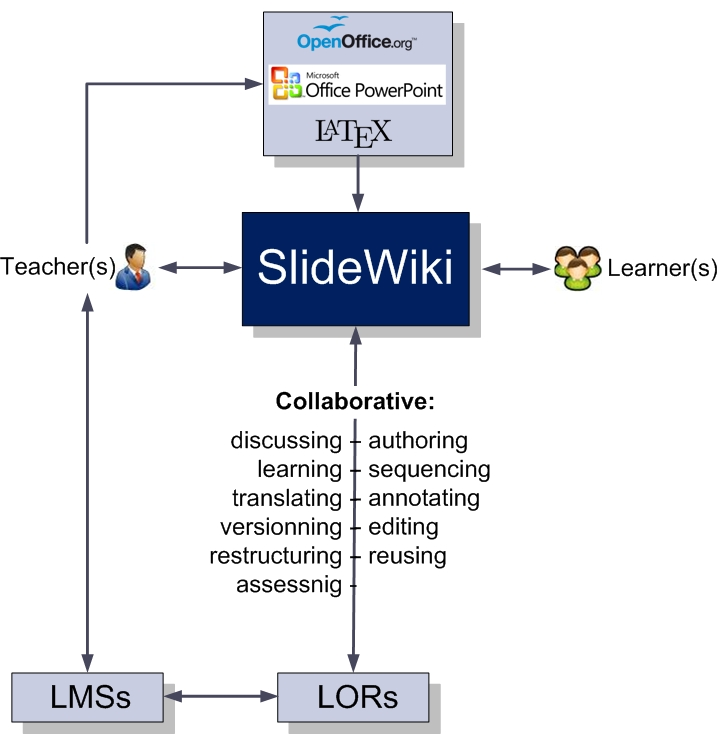
\includegraphics[width=0.6\columnwidth]{images/conceptual_scheme.jpg}
	\caption{SlideWiki conceptual scheme.}
	\label{fig:slidewiki_scheme}
\end{figure}

\section{SlideWiki Architecture, Functionality and User Interface}
\label{sec:architecture}

SlideWiki deals with two types of (semi-)structured learning objects: slide presentations and assessment tests.
The content is organized according to the \emph{COSMEC} concept.
Slide presentations are represented as a combination of individual slides (consisting mainly of HTML snippets, SVG images and meta-data), individual decks (ordered sequences of slides and sub-decks), themes (which are associated as default styles with decks and users) and media assets (which are used within slides).
The self-assessment test sets combine individual tests (which can be organized manually by user or created automatically in accordance with the deck structure and content), questions for the slide material assigned to certain slides (which are part of tests) and answers (which are part of the questions).

The SlideWiki platform is built on top of the LAMP~\footnote{Linux-Apache-MySQL-PHP} technology stack where a relational approach (implemented by MySQL RDBMS) is used to implement the conceptual WikiApp data model of SlideWiki.
The SlideWiki application makes extensive use of the model-view-controller (MVC) architecture pattern, as depicted at \autoref{fig:slidewiki_architecture}.
The MVC architecture enables the decoupling of the user interface, program logic and database controllers and thus allows developers to maintain each of these components separately.

\begin{figure}[tb]
\centering
	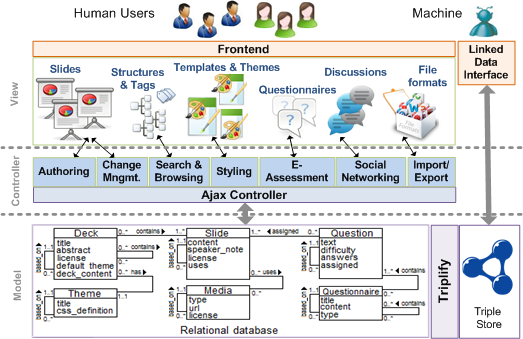
\includegraphics[width=1\columnwidth]{images/architecture.png}
	\caption{SlideWiki architecture overview.}
	\label{fig:slidewiki_architecture}
\end{figure}

SlideWiki makes extensive use of HTML5 features to provide users with intuitive and responsive interfaces.
In addition to the overall MVC architecture, SlideWiki utilizes a \emph{client-side MVC} approach (implemented in JavaScript and running inside the users Web browser).
The client-side MVC handler as (singleton) controller listens to the hash fragment of the requested URLs and once a change has occurred the handler triggers the corresponding actions.
Each action has a JavaScript template (implemented using \textit{jQuery templates}) with the corresponding variable place holders.
For each action an Ajax call is made and the results are returned to the controller in JSON format.
Subsequently, the controller fills the templates with the results and renders them in the browser.

Additionally, SlideWiki supports \emph{progressive loading} of presentations to guarantee the scalability when a large presentation is loaded.
Progressive loading is a design pattern for web applications which adds content to a web page incrementally. 
It results in gradually increasing the workload over time when loading a large presentation thereby improving the performance of the system.

In the section we discuss the design solutions and implementation of main SlideWiki features. 

\subsection{Content Development.}
\label{sec:content_development_implementation}

Being a wiki, the SlideWiki platform supposes the prevalence of the content over format.
Due to this, we were strongly focused on facilitation of the slide content editing process, trying to minimize the complications of slide content format.
This means, that in oppose to desktop single-user slide editing applications (like Microsoft PowerPoint), we do not work with slide layouts.
Instead, we operate on the slide content similarly to Microsoft Word, allowing embedding media within the textual blocks.
Nevertheless, SlideWiki allows to individualize slide formatting by applying style sheets.
Moreover, the SlideWiki users are able to edit, share and reuse their own style sheets in the same manner as they share and reuse the content pieces.

In the section we discuss the tools supporting the authoring of slides and collaboration on them in detail.

\paragraph{Authoring}
SlideWiki employs an inline HTML5 based WYSIWYG (What-You-See-Is-What-You-Get) text editor for authoring the presentation slides~(cf. \autoref{fig:screenshot}, image 1).
Using this approach, users will see the slideshow output at the same time as they are authoring their slides.
The editor is implemented based on ALOHA editor\footnote{\url{http://aloha-editor.org/}} extended with some additional features such as image manager, source manager, equation editor.

The inline editor uses SVG images for drawing shapes on slide canvas.
Editing SVG images is supported by SVG-edit\footnote{http://code.google.com/p/svg-edit/} with some predefined shapes which are commonly used in presentations.
We gave chosen the SVG format due to the open XML-based encoding of the images it creates.
This is especially important for the slide localization, as the textual content of the SVG images can be picked out the rest code blocks and translated.

For logical structuring of presentations, SlideWiki utilizes a tree structure in which users can append new or existing slides/decks and drag \& drop items for positioning.
When creating presentation decks, users can assign appropriate tags as well as footer text, default theme/transition, abstract and additional meta-data to the deck.

SlideWiki follows the ``anyone can edit'' philosophy of Wiki for creating synergistic presentations.
In order to manage the changes made by users, SlideWiki defines a revisioning system as described in the following.

\paragraph{Change Management.}
\label{par:change_management}
\begin{figure}[htb]
	\centering
		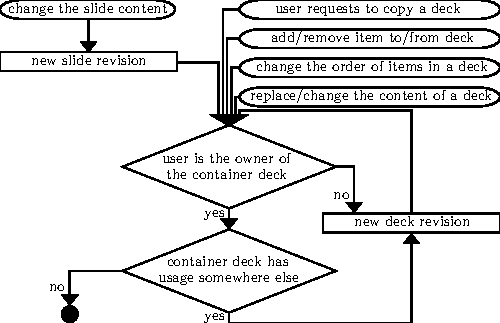
\includegraphics[width=.8\columnwidth]{images/revisions.pdf}
	\caption{Decision flow during the creation of new slide and deck revisions.}
	\label{fig:revisions}
\end{figure}

Revision control is natively supported by WikiApp data model.
We just define rules and restrictions to increase the performance.
There are different circumstances in SlideWiki for which new slide or deck revisions have to be created.
For decks, however, the situation is slightly more complicated, since we wanted to avoid an uncontrolled proliferation of deck revisions.
This would, however, happen due to the fact, that every change of a slide would also trigger the creation of a new deck revision for all the decks the slide is a part of.
Hence, we follow a more retentive strategy.
We identified three situations which have to cause the creation of new revisions:
\begin{itemize}
	\item The user specifically requests to create a new deck revision.
	\item The content of a deck is modified (e.g. slide order is changed, change in slides content, adding or deleting slides to/from the deck, replacing a deck content with new content, etc.) by a user which is neither the owner of a deck nor a member of the deck's editor group.
	\item The content of a deck is modified by the owner of a deck but the deck is used somewhere else.
\end{itemize}
The decision flow is presented in \autoref{fig:revisions}.
In addition, when creating a new deck revision, we always need to recursively spread the change into the parent decks and create new revisions for them if necessary.

\paragraph{Styling.}
In order to create flexible and dynamic templates and styles for presentations, SlideWiki utilizes \emph{Saas} (Syntactically Awesome Stylesheets) language\footnote{\url{http://sass-lang.com/}}.
Sass extends CSS by providing several mechanisms available in programming languages, particularly object-oriented languages, but not available in CSS3 itself.
When Sass script is interpreted, it creates blocks of CSS rules for various selectors as defined by the Sass file.
Using Saas, SlideWiki users can easily create and reuse presentation themes and transitions.


\begin{figure*}[t!]
	\centering
		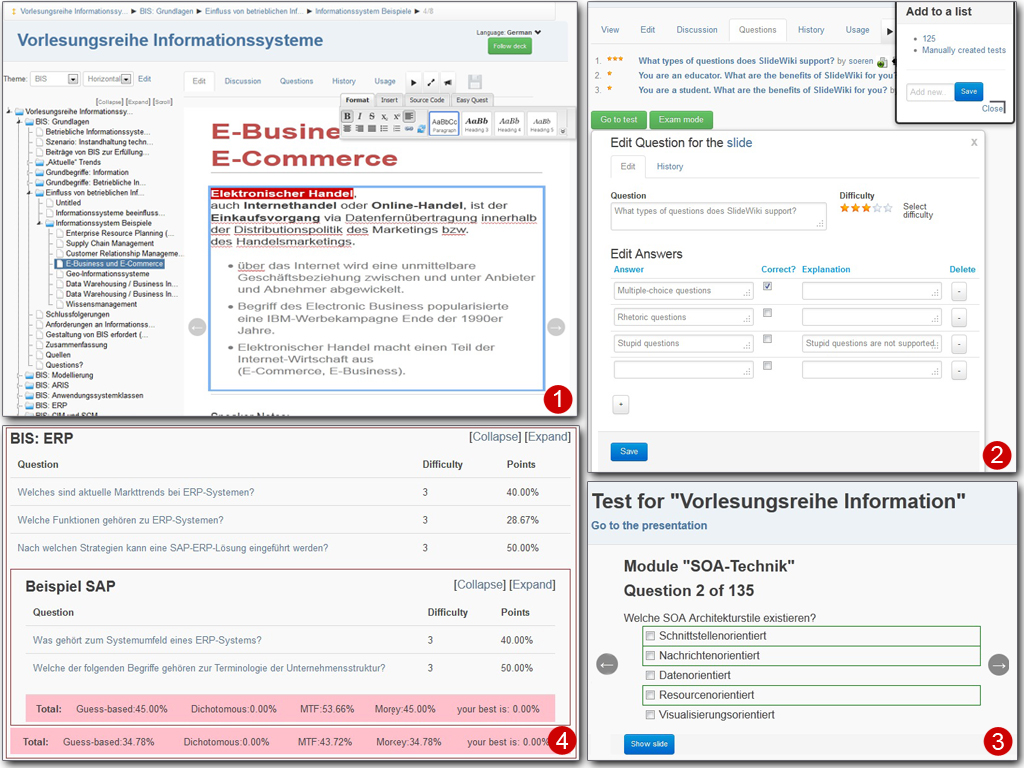
\includegraphics[width=\textwidth]{images/screenshot1.jpg}
	\caption{Four screenshots of SlideWiki features. \textit{\textbf{1} - Tree structure of the presentation, inline WYSIWYG editor; \textbf{2} - Editing of a question and manual assigning to a test using lists; \textbf{3} - Question in learning mode with correct answers displayed; \textbf{4} - Module-based scoring of an assessment test.}}
	\label{fig:screenshot}
\end{figure*}


\subsection{Content Migration.}
\label{sec:content_migration}
Keeping up-to-date with these latest developments and trends in online education, the SlideWiki platform has been developed to target all the widely used and emerging educational channels, in order to maximize its outreach and impact to educators and learners worldwide.
The flexible WikiApp data model allows to fully integrate SlideWiki with LMSs, MOOC platforms, as well as social networks and eBooks.
This integration will ensure that the learning resources developed with the use of the SlideWiki platform are delivered via a variety of educational channels that address different learning contexts, pedagogical and technological requirements, and learning communities. 

In the section we describe the implementation of WikiApp data model for both relational databases and RDF. 
We discuss as well bottlenecks and deficiencies we met during the implementation.
We as well describe the conversion of SlideWiki content into SCOs, that allows to publish the content in a wide variety of existing educational platforms, such as Moodle.

\subsubsection{Data Model for Relational Database}
\label{subsec:datamodel_rdb}

Using the previously discussed WikiApp data model (see \autoref{sec:wikiapp}) we have succeeded to implement the following principles on SlideWiki platform:
\begin{itemize}
\item Provenance: The origin and creation context of all information should be preserved and well documented.
\item Transparency, openness and peer-review: Content should be visible and easily observable for the largest possible audience, thus facilitating review and quality improvements.
\item Simplicity: The implementations should be simple to build and use.
\item Social Collaboration: Following other users, watching the evolution of content as well as reusing and repurposing of content in social collaboration networks is at the heart of data model.
\item Scalability: The implementations should be scalable and be implementable according to established Web application development practices.
\end{itemize}

SlideWiki example application uses two implementations of WikiApp data model. 
The first implementation is used for managing slides and presentations. 
It includes individual slides (consisting mainly of HTML snippets, SVG images and meta-data), decks (being ordered sequences of slides and sub-decks), themes (which are associated as default styles with decks and users) and media assets (which are used within slides). 
The second implementation was developed for managing questions and questionnaires (tests).
It includes questions for the slide material (the question is assigned to all slide revisions), questionnaires (which could be organized manually by user or created automatically in accordance with the deck content), and answers (which are the part of the questions).

We implicitly connected these two WikiApp instances by adding two relations.
Firstly, we assigned questions to slides.
Thus, during the learning process users are able to try answer the questionnaires and have a look the assigned slide if necessary.
The important issue here is that we assign question not to individual slide revision, but for the slide itself.
This decision gives an opportunity to create new slide revision, that already has a list of questions, collected from other revisions.
Secondly, we assigned questionnaires to concrete deck revisions.
Thus automatically created test saves the structure of deck revision, which it is assigned to.
This allows us to use module-based assessment to score the test results.
The following two diagram \autoref{fig:object-model}) illustrates the implementation of WikiApp in SlideWiki.
These two special relations are indicated on the example object diagram by the dashed arrows.

\begin{figure}[htb]
	\centering
		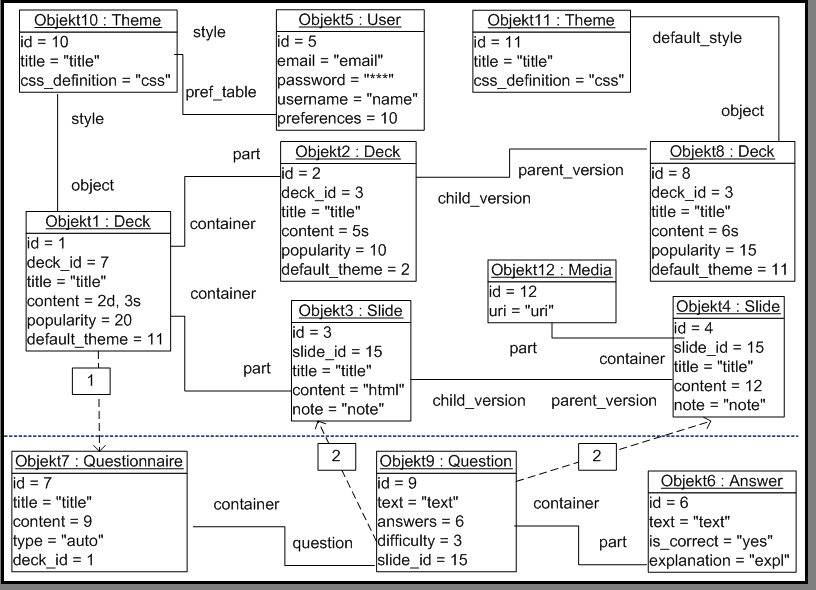
\includegraphics[width=\columnwidth]{images/object_diagramm.png}
	\caption{Example object diagram for Slidewiki. \textit{\textbf{1} - connection between questionnaires and deck revisions to enable module-based scoring; \textbf{2} - connection between questions and slides to allow users see the related material when answering the questionnaires}}
	\label{fig:object-model}
\end{figure}


The current database (see also \autoref{fig:mysql_tables}) consists of 30 tables interconnected by primary or foreign keys:


\begin{table}[!ht]

\begin{tabulary}{1\columnwidth}{ll}
\toprule
\textbf{Table} & \textbf{Function} \\
\midrule

Slide & describes the original slide\\
Slide\_revision & describes the revisions of the original slide\\
Deck & describes the original deck containing a set of slides\\
Deck\_revision & describes the revisions of the original deck\\
Deck\_content & describes the organization of content in a deck\\
Questions & describes multiple-choice questions associated to a slide\\
Answers & describes answers to a question\\
Doubtful & describes the reasons for questions reported by users as doubtful\\
Users & describes the users of platform\\
User\_group & describes different user groups on the platform\\
User\_tests & describes the evaluation test created by a user\\
Test\_content & describes the evaluation test as a set of questions\\
Test\_results & describes the results of an evaluation test\\
Style & describes presentation themes \\
Transition & describes transition effects used in presentations\\
Impress\_transition & describes a special type of transitions\\
Comment & describes user-added comments on a slide or deck\\
Tag& describes keywords assigned to an item (i.e. slide, deck, etc.)\\
Brand & describes branding ads for presentations\\
Message & describes messages communicated between platform users\\
Media& describes media items used in a presentation\\
Medial\_relations & describes the relation between media and the associated item\\
Subscription & describes the user-subscription to a certain slide/deck\\
Badge & describes a user badge\\
Badge\_import\_details & describes the badge associated items\\
Notifications & describes user notifications\\
Preference & describes preferences for user profiling\\
Short\_urls & describes the URLs for search engine optimization\\
Testing & describes performance tests on the platform\\
Translation\_cronjobs & describes translation jobs to be sent to external translation services \\

\bottomrule


\end{tabulary}
\caption{Description of SlideWiki Database Tables}
\label{tab:mysql_tables}
\end{table}





\begin{figure}[!htb]
	\centering
		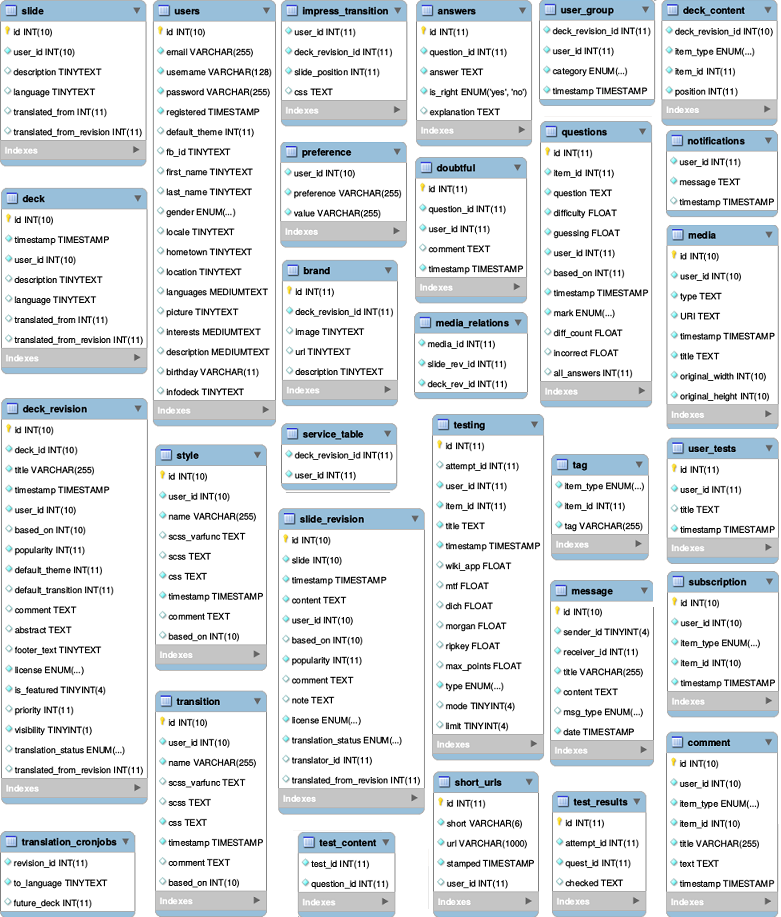
\includegraphics[width=\columnwidth]{images/erm_OLD2.png}
		\caption{An overview of SlideWiki MySQL tables}
	\label{fig:mysql_tables}
\end{figure}


 

\subsubsection{Data Model for RDF}
\label{sec:data_model_rdf}

In order the OER movement to fully success, the OERs have to be searchable and re-usable, in other words the interoperable.
In order to ensure the interoperability, a number of competing approaches, metadata schemas and interface mechanisms was developed the last decade. 
For example, Dublin Core~\footnote{\url{http://dublincore.org/documents/dces/}}, IEEE Learning Object Metadata (LOM)~\cite{learning2002ieee} or ADL SCORM~\footnote{\url{http://www.adlnet.org/}} standards and query interface mechanisms such as OAI-PMH~\footnote{\url{http://www.openarchives.org/pmh/}} or SQI~\footnote{\url{http://www.cen-ltso.net/main.aspx?put=859}}.
However, so far Web-scale integration of resources is not facilitated, mainly due to the lack of commonly shared principles, datasets and schemas~\cite{Dietze:2012:LEI:2245276.2245347}.
At the same time, the Linked Data approach has emerged as the de-facto standard for sharing data on the Web, offering a large potential to solve interoperability issues of any type of digital content.
Thus, we consider the publishing content and its metadata as linked data to be the crucial requirement for the OER.

In order to publish the SlideWiki content in accessible way, we have adapted the developed WikiApp data model for linked data. 
We based the data model on three newly created ontologies: (i) WA ontology~\footnote{\url{http://slidewiki.org/rdf/wa}} models the WikiApp data model and can be reused in any type of WikiApp implementation; (ii) SW ontology~\footnote{\url{http://slidewiki.org/rdf/sw}} models the base SlideWiki relations between content objects and users and (iii) SA ontology~\footnote{\url{http://slidewiki.org/rdf/sa}} models the self-assessment items and can be reused for other e-assessment data mapping.

As there are no ontologies for modeling e-learning objects available, the number of reused properties and classes is not high.
However, we have reused properties from three widely accepted ontologies: 

\begin{itemize}
\item Dublin Core Metadata Initiative Terms (DCMI-TERMS)~\footnote{\url{http://dublincore.org/documents/dcmi-terms/}} is a set of vocabularies which includes the elements from DublinCore, as well as sets of resource classes (including the DCMI Type Vocabulary [DCMI-TYPE]), vocabulary encoding schemes, and syntax encoding schemes.
The terms in DCMI vocabularies are intended to be used in combination with terms from other, compatible vocabularies in the context of application profiles and on the basis of the DCMI Abstract Model [DCAM].
DublinCore (DC) is a vocabulary of fifteen properties for use in resource description.
DC is a simple yet flexible metadata standard, intended to describe a wide variety of resources.

\item{Friend Of A Friend (FOAF)~\footnote{\url{http://www.foaf-project.org/}}} is an ontology describing persons, their activities and their relations to other people and objects.
As used in most of the existing vocabularies, FOAF is a common way to add general information to persons and organizations.
FOAF is one of the key components of the WebID~\footnote{\url{https://www.w3.org/2005/Incubator/webid/}} specifications, and its support by browsers and web-services grows fast.
For example, the Live Journal~\footnote{\url{http://www.livejournal.com/}} and DeadJournal~\footnote{\url{http://www.deadjournal.com/}} blogging sites support FOAF profiles for all their members, My Opera community supports FOAF profiles for members as well as groups, FOAF support is present on Identi.ca, FriendFeed, WordPress and TypePad services. Yandex blog search platform supports search over FOAF profile information.
Prominent client-side FOAF support is available in Safari, Firefox and Google Chrome web browsers. 

\item{Provenance Ontology (PROV-O)~\footnote{\url{https://www.w3.org/TR/prov-o/}}} provides a set of classes, properties, and restrictions that can be used to represent and interchange provenance information generated in different systems and under different contexts. 
Provenance is a critical ingredient for establishing trust of published scientific content.
This is true whether we are considering a data set, a computational workflow, a peer-reviewed publication or a simple scientific claim with supportive evidence.
It is a domain-independent and general-purpose ontology and it allows and encourages for extensions to cover more specific needs. 
In particular, to track authoring and versioning information of content pieces, PROV-O provides a basic methodology but not any specific classes and properties for identifying or distinguishing between the various roles assumed by agents manipulating digital artifacts, such as author, contributor and curator.

\end{itemize}

Additionally, the W3C recommended ontologies are reused to model the CSS styles attached to the content objects~\footnote{\url{http://www.w3.org/ns/oa}} and the textual content of the objects~\footnote{\url{http://www.w3.org/2011/content}}.

Following the WikiApp data model formalization, the core of the WA ontology is built on three main classes: (1) \emph{wa:Container} which corresponds to the \emph{Content Type} concept, (2) \emph{wa:ContentObject} for storing the content objects and all kinds of relations between them and (3) \emph{wa:User}, a subclass of \emph{foaf:Person}.
Being an implementation of WikiApp data model, the ontology requires each content object to have only the \emph{dcterms:created} property specified. 
This ensures high flexibility and interoperability of the ontology, making it easy to be reused in a wide range of applications.

The core relations between content objects can be defined by using one out of four properties.

\begin{itemize}
\item \textbf{\emph{prov:wasRevisionOf}}~\footnote{\url{http://www.w3.org/ns/prov\#wasRevisionOf}}.
The PROV ontology defines revision as a derivation for which the resulting entity is a revised version of some original.
The implication here is that the resulting entity contains substantial content from the original.
Revision is a particular case of derivation, that is reflected by the \emph{prov:wasRevisionOf} property being a subclass of \emph{prov:wasDerivedFrom} property.
The suitable semantics of the property, its quality and popularity of the PROV ontology itself led us to the decision to reuse it instead of defining a new one.
In order to simplify the usage of the future datasets, we define as well the inverted property \emph{wa:hasRevisions}.

\item \textbf{\emph{wa:translationOf}}. 
Despite the fact the integration of PROV vocabulary allowed us to use the \emph{prov:hadPrimarySource property} for defining the relation between translation and its original, we have decided not to reuse the property.
The reason for that decision is its potentially ambiguous meaning.
For example, in the SlideWiki example implementation a slide presentation can have an assigned source, that is usually a textbook the slides are based on.
In order to overcome the ambiguity we defined an own property, making it however a subproperty of \emph{prov:wasDerivedFrom}. 
This allows us to use all the semantics defined for the PROV vocabulary and at the same time allows to add own specifications.
\item \textbf{\emph{dcterms:hasPart}}~\footnote{\url{http://dublincore.org/documents/dcmi-terms/\#terms-hasPart}}.
We reuse the property as well as its inversion \emph{dcterms:isPartOf} to define the \emph{part-of} relationship between two content objects.

\item \textbf{\emph{wa:assignedTo}}
The property defines the many to one relationship between two content objects.
Its common usage includes the assigning comments, notes or questions to other content objects.
\end{itemize}
  

\begin{figure}[htb]
	\centering
		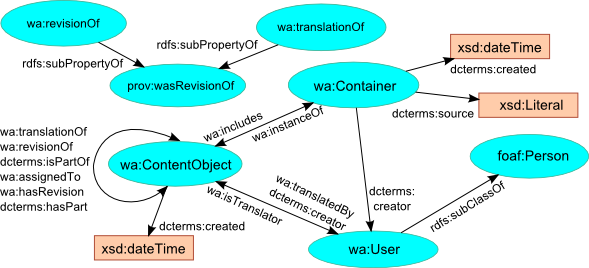
\includegraphics[width=\textwidth]{images/wa_ontology.png}
	\caption{WikiApp data model implemented as an ontology}
	\label{fig:wa_ontology}
\end{figure}

The complete SlideWiki knowledge graph is presented in~\autoref{sec:app1}.

\subsubsection{RDB2RDF Conversion}
\label{sec:RDB2RDF}

\todo{r2rml standard}

An RDB2RDF mapping can either be represented as a set of customized rules or through a generic set of rules (as defined by the W3C Direct Mapping standard~\footnote{\url{https://www.w3.org/TR/rdb-direct-mapping/}}).
Often, the output of a Direct Mapping may not be useful, that is, it may not adequately take the structural and/or semantic complexity of the database schema into account.
Due to the complexity of the SlideWiki data model, we have concluded that not using the customized rules would lead to a loss of resulting data quality. 

A large number of tools for mapping relational data to RDF exist already\footnote{One of the listings is available at \url{https://github.com/timrdf/csv2rdf4lod-automation/wiki/Alternative-Tabular-to-RDF-converters}.}, they implement different mapping approaches, often allowing to customize the mapping. Customized mappings in their turn can be represented in different material forms (proprietary formats, visual diagrams, tables, etc.).
Languages for representing customized mappings have been surveyed in \cite{spanos2012bringing}.
Until recently, no standard representation language for customized RDB2RDF mappings existed.
However, in 2012 the W3C RDB2RDF Working Group has released recommendations for the Relational Database to RDF Mapping Language (R2RML)~\footnote{\url{https://www.w3.org/TR/r2rml/}}.
As it is the only mapping language that has been standardized to date, we do not consider usage of other (proprietary) formats reasonable. 

\begin{table*}[!ht]

	\centering		
	\begin{tabulary}{\textwidth}{LLL}
	\toprule
		\textbf{{Requirement}} & \textbf{{Description}} & \textbf{{Measure}} \\
		\midrule
		
		\multicolumn{3}{c}{\textbf{Quality of the mapping implementation and representation}} \\
\hline
		\textbf{Data accessibility} &
Describes how the mapping result can be accessed. 
		 & ETL/on-demand/both\\
\hline
		\textbf{Standard compliance} &
Characterizes if the mapping representation is standard compliant.
		 & boolean \\
\hline
		 
		\multicolumn{3}{c}{\textbf{Faithfulness of the output}} \\		
\hline
		\textbf{Coverage} & Characterizes the mapping completeness  & percentage of DB columns mapped  \\
\hline
		\textbf{Accuracy of data representation} & Characterizes the mapping correctness & percentage of correctly mapped DB columns \\
\hline
		\textbf{Incorporation of domain semantics} & Shows level of domain semantics incorporation & percentage of properties that link to the results of SQL queries \\
\hline
		
		\multicolumn{3}{c}{\textbf{Quality of the output}} \\		
\hline
		\textbf{Simplicity} & Shows the simplicity of SPARQL queries returning the frequently demanded values & percentage of complex SQL queries results integrated into the mapping \\
\hline
		\textbf{Data quality} & Characterizes the quality of output data & aggregation of linked data quality metrics \\
\hline
		\textbf{Data integration} & Characterizes the interlinking degree of the output data & percentage of external instances integrated into the resultant dataset\\	
\hline
		
		\multicolumn{3}{c}{\textbf{Interoperability}} \\		
\hline
		\textbf{Reuse of existing ontologies} & Shows the amount of reused vocabulary elements & percentage of reused properties and classes\\
\hline
		\textbf{Quality of reused vocabulary elements} & Characterizes the quality of chosen for reuse properties and classes & accumulated quality and popularity of reused vocabulary elements \\
\hline
		\textbf{Accuracy of reused properties} & Characterizes the accuracy of properties reuse & percentage of accurately reused properties \\
\hline
		\textbf{Accuracy of reused classes} & Characterizes the accuracy of classes reuse & percentage of accurately reused classes  \\
\hline
		\textbf{Quality of declared classes/properties} & Shows the quality of ontology documentation & accumulated quality of declared classes/properties\\
\hline
	
	\end{tabulary}
		
	\caption{Summary table of the proposed metrics system}
	\label{tab:rdb2rdf_summarytable}
\end{table*}

The trial conversion of the SlideWiki relational data to RDF using R2RML has already been proceeded.
We have used an open-source Java-based tool \emph{SparqlMap}\footnote{\url{http://aksw.org/Projects/SparqlMap.html}} that allows the execution of a SPARQL query fully inside a relational database and does not require dumping the data first.
The tool takes as an input a list of settings (mainly related to the database connection) and the previously defined R2RML mapping representation.
Based on those, SparqlMap outputs set of triples in Turtle notation~\footnote{\url{https://www.w3.org/TeamSubmission/turtle/}}.
The translation is a light-weight process with low requirements on processing power.
The mapping of the relational database is expressed using R2RML~\cite{unbehauen2012accessing}.

SparqlMap allows to establish the access to the resulting triples using two main paradigms: (i) Extract Transform Load (ETL) and (ii) on-demand mapping.
ETL means physically storing triples produced from relational data in an RDF store.
The disadvantage of ETL is that, whenever the RDB is updated, you have to re-run the entire ETL process, even if just one RDB record has changed, carrying out an often redundant synchronization process.
However, in the ETL case nothing more than the RDF store is needed to answer a query.
On-demand mapping is realized by translating a SPARQL query into one or more SQL queries at query-time, evaluating these against (a set of) unmodified relational database(s) and constructing a SPARQL result set from the result sets of such SQL queries.
In contrast to the ETL implementation, on-demand mapping requires more resources for processing each query.
However, the on-demand implementation does not face the synchronization issue and does not replicate the data.
In the light of these advantages and disadvantages, we have decided that the best solution is to implement the both data access approaches.

\begin{table*}[!ht]
\centering
\setlength{\tabcolsep}{4pt}
\begin{tabular}{p{0.05\linewidth}|p{0.28\linewidth}|p{0.11\linewidth}|p{0.09\linewidth}|p{0.06\linewidth}|p{0.11\linewidth}|p{0.09\linewidth}|p{0.06\linewidth}}

\rowcolor[gray]{.7}
\hline
\textbf{$W$}  &\textbf{Requirement} & \textbf{$Potential_1$} & \textbf{$Actual_1$} & \textbf{$i_1$} & \textbf{$Potential_2$} & \textbf{$Actual_2$} & \textbf{$i_2$} \\
\hline

\rowcolor[gray]{.9}
\textbf{0.1} & \multicolumn{3}{l|}{\textbf{Quality of mapping}} &\textbf{1} & & & \textbf{1}\\

0.5 & - data accessibility & - & both & 1  & - & both & 1  \\
0.5 & - representation & - & R2RML & 1  & - & R2RML & 1 \\

\rowcolor[gray]{.9}
\textbf{0.2} & \multicolumn{3}{l|}{\textbf{Faithfulness of output}} &  \textbf{0.7}  & & & \textbf{0.76} \\

0.4 & \colorbox{gray!50}{- coverage} & 169 & 78 & \colorbox{gray!50}{0.46}  & 169 & 100 & 0.59 \\
0.5 & - accuracy & 0 & 0 &  1  &  0 & 0 & 1 \\
0.1 & - domain semantic & 39 & 7 & 0.18   & 43 & 9 & 0.21 \\

\rowcolor[gray]{.9}
\textbf{0.3} & \multicolumn{3}{l|}{\textbf{Quality of output}} &  \textbf{0.51}  & & & \textbf{0.913} \\

0.3 & - simplicity & 18  & 14 &  0.78  & 18 & 14 & 0.78  \\
0.4 & \colorbox{gray!50}{- data quality} & 6  & 4.5 &  \colorbox{gray!50}{0.75}  & 6 & 6 & 1  \\
0.3 & \colorbox{gray!50}{- data integration} & 1 & 0 &  \colorbox{gray!50}{0}  & 1 & 1 & 1 \\

\rowcolor[gray]{.9}
\textbf{0.4} & \multicolumn{3}{l|}{\textbf{Interoperability}} &  \textbf{0.9}   & & & \textbf{0.91} \\

0.15 & - reuse of properties & 39 & 24 &  0.615  & 44 & 28 & 0.64\\
0.05 & - reuse of classes & 10 & 2 &  0.2  & 11 & 3 & 0.27\\
0.15 & - quality of reused properties & 24 & 24 &  1   & 28 & 28 & 1 \\
0.3 & - accuracy of reused properties & 24 & 24 &  1  &  28 & 28 & 1 \\
0.15 & - quality of reused classes & 2 & 2 &  1   &  3 &3 & 1 \\
0.1 & - accuracy of reused classes & 2 & 2 &  1  & 3 & 3 &1 \\
0.1 & - quality of newly created properties & 15 & 15 &  1   & 16 & 16 &1 \\


\rowcolor[gray]{.7}
\hline
\multicolumn{4}{r|}{\textbf{Total}}& \textbf{0.778}  & & & \textbf{0.95} \\

\end{tabular}
\caption{Mapping quality evaluation.}
\label{tab:qual_eval}
\scriptsize{i - the index of evaluated requirement, W - weight of the index in the result mapping quality evaluation. The metrics with gray background were improved in the final mapping.}

\end{table*}

We have created the R2RML file needed to customize the mapping in three steps.
First, we have created the initial mapping, using common knowledge of linked data quality.
On the second step, we have evaluated the mapping using our previously developed metric system (see~\autoref{sec:app_rdb2rdf}), summarized in~\autoref{tab:rdb2rdf_summarytable} with minor changes.
And finally, we have improved the initial mapping based on the evaluation.
The extractions of the final R2RML file we created are listed in ~\autoref{app1:r2rml}

In~\autoref{tab:qual_eval} we summarize the results of the evaluation for both initially created and improved mappings.
The metrics that we consider to be insufficiently good after the first iteration are shown with the gray background.
Based on the discussion, we improved the quality of metrics from output faithfulness and quality dimensions, as discussed below:

\begin{enumerate} 

\item{\emph{Quality of mapping implementation.}}
As we used R2RML file to represent the mapping and established both ETL and on-demand data access, the index of mapping implementation quality is maximal (thus, equal to 1).

\item{\emph{Faithfulness of output.}}
As SlideWiki contains a lot of usage statistics and service tables (private messages, data for cronjobs etc.), the index of coverage is quite low.
However, during the assessment we took the decision to include two additional tables into the mapping.
As we did not have any digital values mapped, the index of accuracy is 1.
SlideWiki is based on a complicated data model.
Thus, while implementing the platform, we tried to hide this complexity from the user as was done while creating the mapping.
This resulted in the index value of domain semantics incorporation equal to 0.18, which we considered sufficient.
According to our weighting, the index of faithfulness reaches 0.7 and should be increased by increasing the index of coverage. 

\item{\emph{Quality of output.}}
To calculate the index of simplicity our domain specialists created a list of frequently used complicated queries (cf.~\autoref{tab:dom_semantics}).
According to the evaluation, the index level of 0.78 was considered to be sufficient.

\begin{table}[!ht]
\centering

\begin{tabular}{p{0.7\linewidth}|p{0.14\linewidth}}

\toprule
\textbf{Query} & \textbf{Incorp.} \\
\midrule
- get content of a deck & 1 \\
- get usage of a deck & 1 \\
- get usage of a slide & 1 \\
- get questions assigned to a deck & 0 \\
- get questions assigned to a slide & 1 \\
- get contributors of a deck & 1 \\
- get contributors of a slide & 0 \\
- get language of a deck & 1 \\
- get language of a slide & 1 \\
- get translations of a deck & 0 \\
- get translations of a slide & 0 \\
- get all revisions of a deck & 1 \\
- get all revisions of a slide & 1 \\
- get tags of a deck & 1 \\
- get comments assigned to a deck & 1 \\
- get comments assigned to a slide & 1 \\
- get content of a user test & 1 \\
- get usage of a question in user tests & 1 \\

\bottomrule
\textbf{18} & \textbf{14} \\
\end{tabular}
\caption{Incorporation of frequently used complicated queries results into the mapping to simplify usage the linked data}
\label{tab:dom_semantics}
\end{table}

We have measured the data quality produced by the mapping using the metric system proposed by ~\cite{Zaveri}.
After the evaluation, the dataset quality produced by the initial mapping was not sufficiently high.
In order to increase the index, we have added machine-readable indication of a license (CC-BY-SA), metadata about publisher and dataset itself.
These actions resulted in improvement of the data quality from the trustfulness aspect. 


\item{\emph{Interoperability.}}
The initial mapping consisted of 10 classes (2 of which were reused) and 39 unique properties (24 reused).
The properties were chosen based on LOV metrics; ranges, domains and comments were taken into account.
For newly created properties dereferencable URIs were created.
This activity resulted in a high level of interoperability.
\end{enumerate}


\subsubsection{SCORM}
\label{sec:SCORM}

\emph{Sharable Content Object Reference Model} (SCORM)~\cite{scorm_specification2011} as one of the community-approved standards, requires the transformation of the learning material into the sequence of annotated \emph{Sharable Content Objects} (SCOs).
The granularity and sequencing of the SCOs should be determined by the content author depending on the audience needs and preferences~\cite{scorm2011}.
Each SCO can include several objects (images, diagrams, text blocks, questions to answer etc.), however, each SCO should be context neutral and should stand alone~\cite{Melon2004}.
Such a structuring optimizes the re-usability while still meets the needs of the learners for whom it was originally intended.

As the content of SlideWiki is semantically structured, it satisfies the requirements of the SCORM standard and the conversion is straightforward.
For now we have implemented a beta-version of the conversion, which produces a structured list of slides followed by a plain list of self-assessment questions attached to each subdeck.
We have tested the produced SCOs in Moodle.
The resulting SCOs keep the content, styling, structure and metadata of the original SlideWiki slides, as shown at \autoref{fig:moodle}.
Thus, a deck is converted to a SCO which can be used as a course module without additional work.
The low efforts needed to implement the conversion prove the flexibility and interoperability of our data model. 

\begin{figure*}[!Ht]
	\centering
		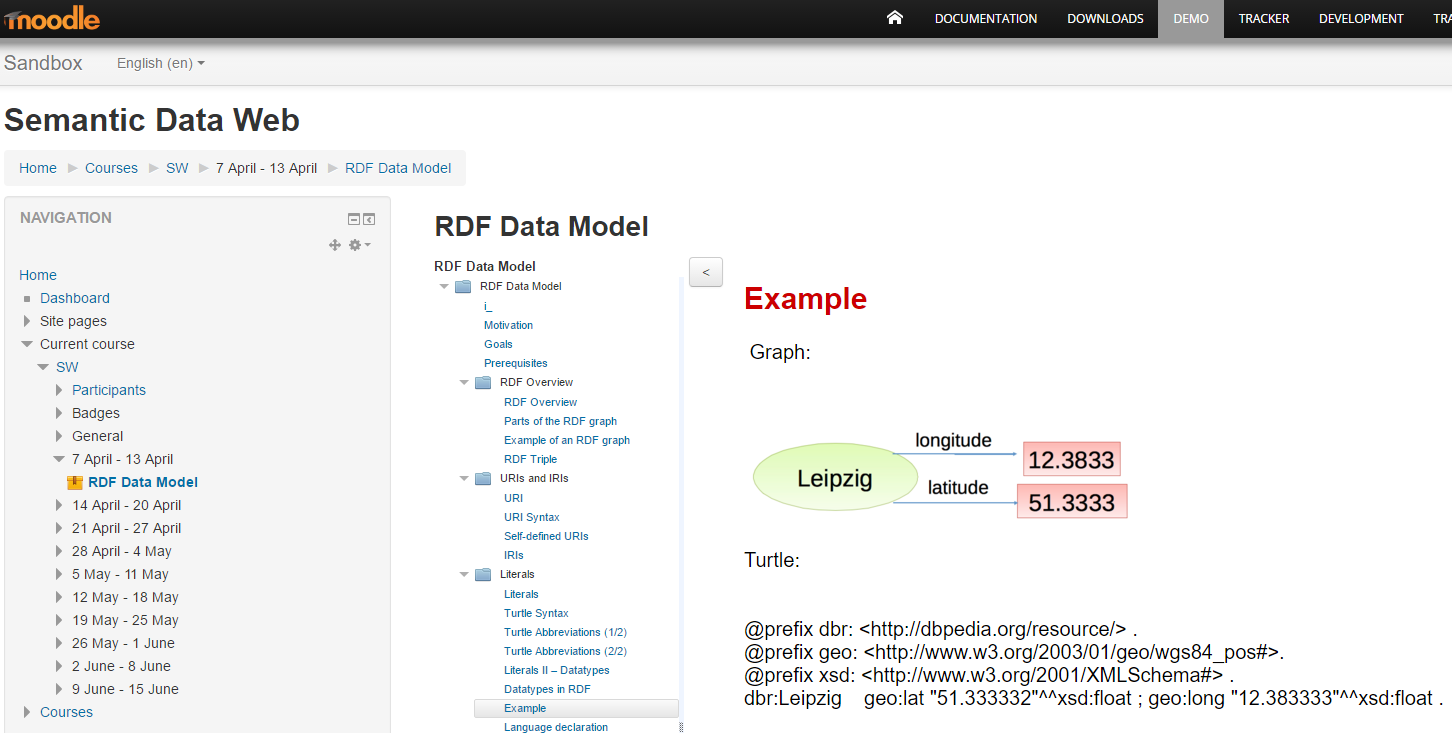
\includegraphics[width=\textwidth]{Images/moodle.png}
	\caption{SlideWiki deck imported in Moodle as a SCORM package}
	\label{fig:moodle}
\end{figure*}

\subsection{Multilinguality}
\label{sec:multilinguality_impl}

The implementation of multilingual content support in SlideWiki is based on the previously described CoSMEC concept and co-evolution paradigm (see \autoref{sec:multilinguality}).
According to the CoSMEC concept, the implementation of co-evolution of source object content and its translations supposes the implementation of three operations: initial translation, synchronization and merging of the revisions.

Our architecture allowed us to implement a \emph{translation} operation backed by the Google Translate service.
After translation into one of 71 currently supported languages, the presentation can be edited, re-structured and reused independently from its source.
The interface for the translation mechanism is depicted at ~\autoref{fig:translation_screen}.

\begin{figure*}[!htb]
	\centering
		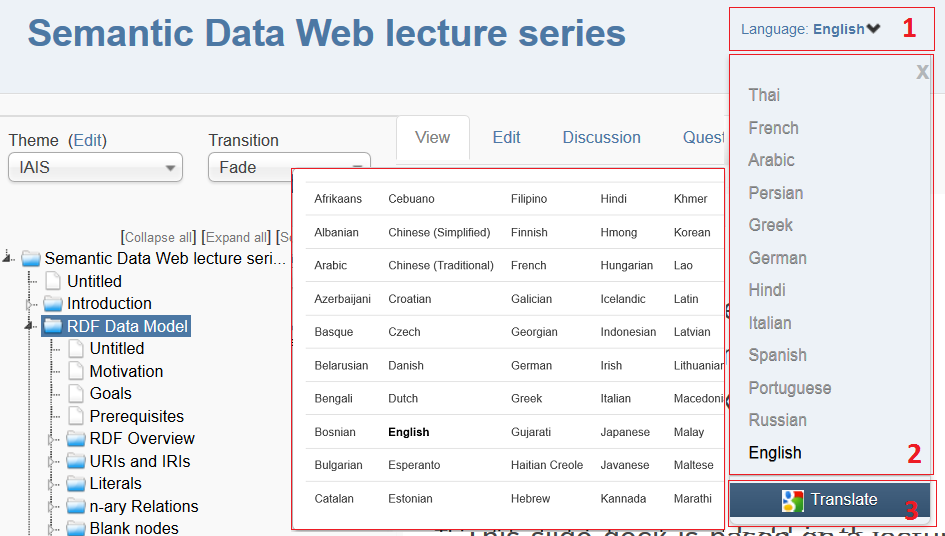
\includegraphics[width=\textwidth]{Images/translation_screen.png}
	\caption{Interface of translations management: 1 - language of selected object; 2 - a drop-down list with links to languages available fro the selected object; 3 - button for translation; 4 - dynamically updated list of the languages supported by Google Translate service}
	\label{fig:translation_screen}
\end{figure*}

To enable \emph{synchronization} of original and translated versions, every further revision of translated objects inherits the link to the source revision (see v2.1 at~\autoref{fig:synchronization}).
The changes in the original version of the object cause the creation of new revision v1.1.
Additionally, users are notified of translations that have become out of sync with the source (exclamation marks in v2.0 and v2.1).


In SlideWiki implementation of the synchronization is slightly different for slides and decks. 
We decided not to implement \emph{manual} synchronization of decks, considering the process to be too complicated for users.
Users can only trigger an \emph{automatic} synchronization.
However, our  data model allows us to get all existing translations for all existing slide revisions.
Then, during an automatic deck synchronization we do not repeatedly translate the slides which have already been translated to the target language before.
Instead, we include in the translation the latest revision of the slide in the target language.
Thus, the synchronization of decks only adds the slides and subdecks that were not included in the source deck at the moment of previous translation.

For the slides both automatic and manual synchronization are enabled.
The users are able to compare v1.0 and v1.1 and decide, either they want to redo the translation (scenario 1 at ~\autoref{fig:synchronization}) or they want to update the content manually (scenario 2).

\begin{figure*}[!ht]
\centering
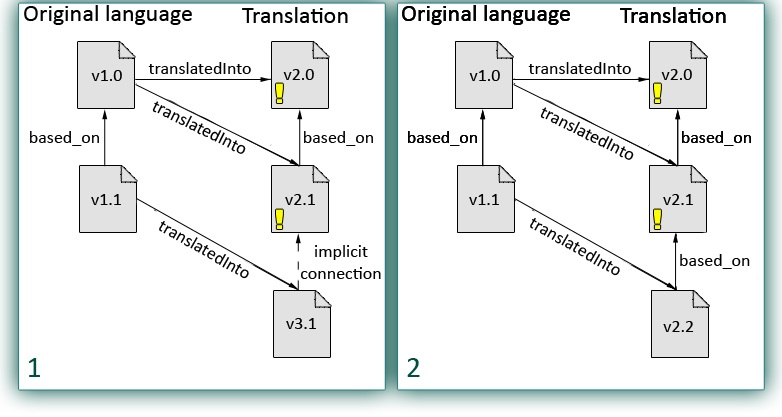
\includegraphics[width=0.8\textwidth]{Images/translation-logic.jpg}\\
\caption{Two scenarios of content synchronization between translation and source: 1 - automatic; 2 - manual synchronization}
\label{fig:synchronization}
\end{figure*}

SlideWiki implements the revision control in accordance with the WikiApp data model, where \emph{merging the revisions} is supported as one of the core operations.
However, as discussed above we defined rules and restrictions to increase the performance.
Namely, we introduced the \emph{content owner} and \emph{member of editor group} roles.
If the changes are made by a user belonging to one of these two roles, the creation of a new \emph{deck revision} is not triggered (the new \emph{slide revision} however is created).
As we allow the owner of a deck revision to change it without the creation of a new revision, it was an important issue whether we should allow the multiple translation of the same revision into the same language or not.
We decided to allow it, however, this led to the situation that we would get several identical presentations with content of bad quality, since it was translated automatically and not edited manually.
However, we could not disable the multiple translations, because in that case it would be impossible for example to get translations of new slides if they were added by the owner.
Thus, merging the revisions became the crucial operation, not only for merging back-translation with the source, but also for merging multiple translations in the same language.
At ~\autoref{fig:merging} we illustrate the interface for comparing and merging deck revisions.

\begin{figure*}[!htb]
	\centering
		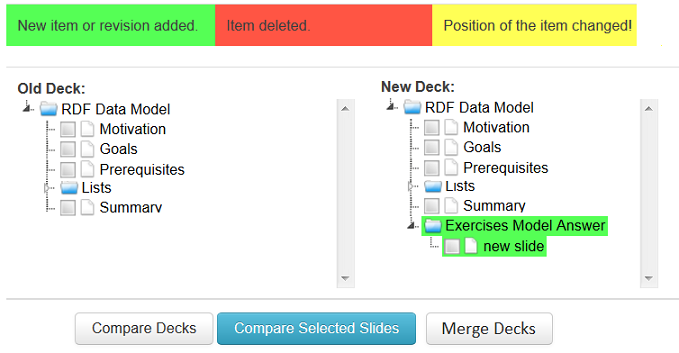
\includegraphics{Images/merging.png}
	\caption{Interface for comparing and merging deck revisions}
	\label{fig:merging}
\end{figure*}

To evaluate the effectiveness of multilinguality support, we collected the statistics of usage the translation tool as well as statistics of the multilingual content it produced.

At ~\autoref{fig:distribution} we present the distribution between original and translated versions in relation to the total number of content objects.
As the WikiApp data model does not enable deletion or update of the content, the graphs can be viewed as time trends. 
The blue line shows an example moment in time, when the SlideWiki database consisted of 16321 slides overall. 
The graphic shows that 78\% of the slides at the moment were in their original language,  22\% were translations and 5\% of total number of slides were revised after translation.
At the same moment, about 35\% of decks were translations.
Thus, the percentage of translated decks increases faster than the same for slides.
This means that the presentations consisting of less than average number of slides are being translated more often.
This can be due to the fact that users want to try the feature before using it on large decks.
However, the assumption needs further investigation.

According to the statistics, the percentage of content created by translation has a strongly increasing trend.
We predict the percentage of translations will soon prevail over the percentage of source objects. 
From one perspective, the prevalence means decreasing the production costs and a large diversity of languages available.
However, from another perspective, it causes the reduction of average content quality, as refining the translation needs time and human resources.
This is illustrated by the decreasing percentage of revised slides in compartment with translated ones. 
The solution is in additional user motivation to put effort in refining the concrete translations according to their knowledge in both domain and languages. 

\begin{figure*}[!ht]
\centering
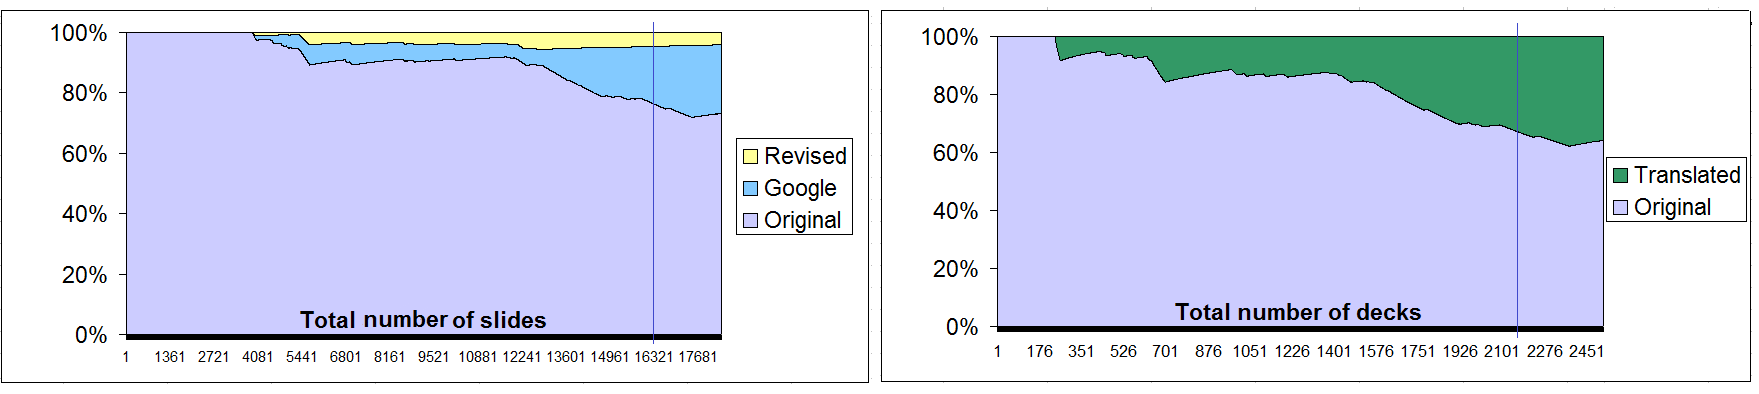
\includegraphics[width=1\textwidth]{Images/translations_number.png}
\caption{Percentage distribution between original and translated versions vs. total number of content objects for slides and decks. Blue line shows an example time moment, discussed in the paragraph above.}
\label{fig:distribution}
\end{figure*}

The diagrams on the~\autoref{fig:distribution3} show the language distributions for decks, slides and visitors (according to Google analytics).
Only unique visitors are counted.
Due to its large percentage, we excluded English language from the resulting diagrams to increase the informativeness. 
The statistics show the visible correlation between number of content objects available in a concrete language and number of visitors speaking the language (for the most of languages).
The results look promising, as they prove the involving of not English-speakers into the global e-learning community activity.
Especially promising looks the fact that more than 13\% of overall visitors belong to developing countries and regions (mostly Eastern Europe and Russia, Turkey, Arabic-speaking countries, Thailand).
We believe that this percentage will increase with increasing the popularity of the source.

\begin{figure*}[!ht]
\centering
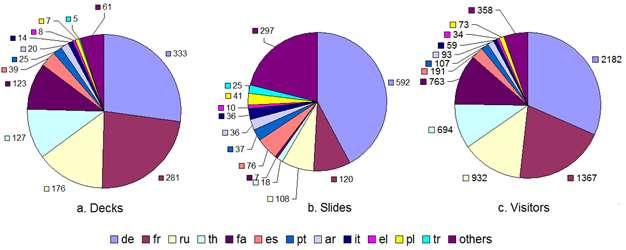
\includegraphics[width=1\textwidth]{Images/languages+visitors.png}
\caption{Distribution of languages for content objects and new visitors}
\label{fig:distribution3}
\end{figure*}

 
\subsection{User Engagement and Social networking}
The theoretical foundations for e-Learning 2.0 are drawn from social constructivism.
It is assumed that students learn as they work together to understand their experiences and create meaning.
In this view, teachers are knowers who craft a curriculum to support a self-directed, collaborative search and discussion for meanings.
Supporting social networking activities in SlideWiki enables students to proactively interact with each other to acquire knowledge.
With the SlideWiki concept we address the following social networking activities:
\begin{itemize}
\item Users can follow individual learning objects as well as other users activities to receive notification messages about their updates.
\item Users can discuss the content of learning objects in a forum-like manner.
\item Users can share the learning objects within their social network websites such as Facebook, Google Plus, LinkedIn, etc.
\item Users can rate the available self-assessment questions in terms of their difficulty and quality.
\end{itemize}

Besides increasing of the learning process quality, social activities improve the quality of the created learning material.
Even when answering a quiz, users can contribute by analyzing the quality of the questions and making suggestions of how to improve them.
Thus, the knowledge is being created not only explicitly by contributors, but also implicitly through discussions, answering the questions of assessment tests, or in other words through native learning activities.


\subsection{E-Learning and E-assessment.}
\label{sec:impl_e-learning}
SlideWiki supports the creation of questionnaires and self-assessment tests from presentation slides.
Questionnaires (like decks and slides) are supported by a revisioning system so that users can create, edit and share questionnaires according to the Wiki collaboration style.
The created questionnaires can be employed for training organization members or to interview prospective members.
Educators can manually or automatically generate evaluation tests from the questionnaires based on their preferences to assess the knowledge of employees to be trained.

Each question has to be assigned to at least one slide.
Important note here, that the question is assigned not to the slide revision, but to slide itself.
Thus, when a new slide revision appears, it continues to include all the list of previously assigned questions.
Questions can be combined into tests.
The \textit{automatically created} tests include the last question revisions from all the slides within the current deck revision.
Manually created tests present a collection of chosen questions and currently cannot be manipulated as objects ~(cf. \autoref{fig:screenshot}, image 2).
Thus, in our implementation only questions and answers have to be placed under the version control.
However, their structure is trivial and the logic of creating their new revisions is intuitive.
We just restricted the number of new revisions to be created similarly with the decks: changes made by the question owner do not trigger a new revision creation.

Students can start a chosen test (manually created or automatically collected) in one of two possible modes: ``learning'' or ``examination''.
In learning mode student can ask to show the slide, to which the question is assigned to remind the material, or simply show the correct answers ~(cf. \autoref{fig:screenshot}, image 3).
Thus, student should not spend time to find the material.
However, after the user asked to show her/him either the slide or correct answers she/he will not get any points for the question.
In examination mode these features are disabled.

After choosing the mode the user can also set up the amount of questions (all, all the difficult or concrete amount) and the order to show them (random or increase the difficulty).
As the amount of questions can differ for the same test, we show the test results as a percentage of the maximum points for exactly this selection of question.

Our architecture allowed us to implement module-based scoring.
Each module of the assessment test presents a sub-deck of the presentation and is scored individually.
Then, all the ``parent'' modules are scored as a sum of ``children'' points and finally the whole test is scored as a sum of all the points for all the modules ~(cf. \autoref{fig:screenshot}, image 4).
To score the results the student (or the teacher) can choose one of five implemented algorithms.
All five algorithms use the dynamically accumulated difficulty $d$ of the question as the number of points for the fully correct response:

\begin{equation}
d = \frac{incorr}{all}
\end{equation}

If the user prefers to use dichotomous scoring, the values of $incorr$ and $all$ mean, respectively, the accumulated number of \textit{incorrect} answers and \textit{all} answers of that question by any of users.
In a case of partial scoring, $incorr$ is determined as follows:
\begin{equation}
incorr = \sum \limits_{i=1}^n(1 - \frac{p_{i}}{d_{i}}) ,
\end{equation}
where $n$ - number of attempts for the question,
$d_{i}$ - difficulty (or maximal points), that the question had at the moment, when the i$ ^{th}$ attempt was made, $p_{i}$ - points obtained in the i$ ^{th}$ attempt

After the difficulty is determined, it's scaled to $(1,d_{max}]$, where $d_{max}$ is the maximal weight, that a question can have.
$d_{max}$ is set up by the system administrator only for the users' comfort.
In SlideWiki we set it up to 5.

After we have studied existing partial scoring algorithms we came to a conclusion about necessity of developing a new one.
We have called it balanced scoring method and give its formal definitions and results of synthetic experiments in \autoref{chapter:self_assessment}.

For evaluation of our algorithm we used a lecture series on ``Business Information Systems''. 
We chose this course since it comprises a large number of definitions and descriptions, which are well suited for the creation of MMQs. 
In total we have created 130 questions.
A course of 30 students was offered to prepare for the final examination using SlideWiki.
Overall, the students made 287 attempts to complete the questionnaire and we collected all their answers (also unfinished assessments) for the evaluation.
After collecting the answers, we implemented all discussed algorithms to score  and compare the results, in particular with regard to the ranking and the mean score.
%To evaluate our approach we have conducted a statistical study, based on the the answers.
The results are summarized in~\autoref{fig:balanced_statistics}.

\begin{figure*}[t!]
	\centering
		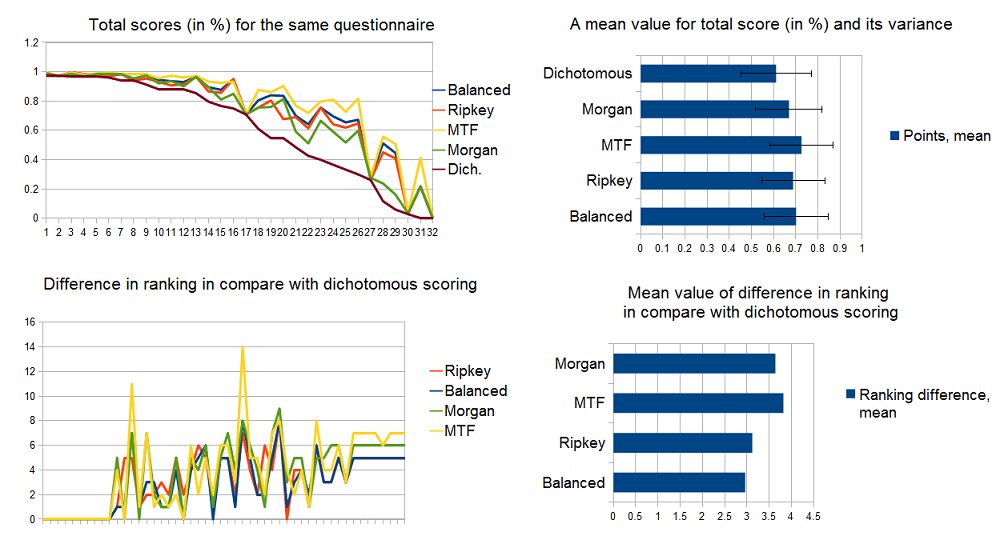
\includegraphics[width=\textwidth]{images/statistics.png}
	\caption{The statistics of the evaluation}
	\label{fig:balanced_statistics}
\end{figure*}

The study aimed to investigate three aspects of the proposed approach:

\begin{itemize}
  \item How severe does the balanced scoring approach penalize?
  \item How does balanced scoring differ from Dichotomous scoring?
  \item How clear were the results scored by the proposed approach for the students?
\end{itemize}

We answer the first question by comparing the scores calculated using all discussed algorithms for the same questionnaire (see \autoref{fig:balanced_statistics}, upper part).
These two diagrams show, that on average the balanced scoring approach penalizes more severely than MTF scoring and less severely than other discussed approaches.
Thus, the users study confirms the findings of our previous synthetic experiment.

We answer the second question by comparing the difference in student ranking.
We rank all assessments based on the individual scores.
That is, assessments with higher scores rank higher than assessments with lower scores and equal scores result in the same ranking.
We compare the rankings of other approaches with the rankings calculated using the dichotomous scoring, since we consider the dichotomous scoring to be the ranking reference.
The two lower diagrams in \autoref{fig:balanced_statistics} show the results of this evaluation.
They show, that the ranking of the balanced scoring approach is the closest to the dichotomous ranking when compared to the other algorithms.

After the end of semester we asked the participants to answer the third question. 
They were offered to evaluate clarity of the results on a five--point scale from "very clear" to "very unclear".
We have collected nine responses, two of them were "neutral", four -- "clear" and three -- "very clear".
This confirms that the results obtained by the balanced scoring method are easy to understand for students.

The proposed approach has a list of restrictions, however it has advantages when compare with the discussed approaches.
One of the main advantages is its clearness for the students, that was proven by the user evaluation presented above.
Also, our approach is based on the mathematical model, it does not suffer from the skewness, as it has the same formula for all cases.
At the same time, the proposed approach recognizes the attempts to guess the correct answer, for example choosing all the possible options.
When compare with the existing approaches, the advantages of the proposed algorithm could be summarized as follows:

\begin{itemize}
  \item The approach allows to score both multiple-mark and conventional multiple-choice questions.
  \item The approach is based on the partial scoring concept.
  \item The algorithm can be easily implemented, it is pure mathematical.
  \item The score does not highly depend on the amount of correct and incorrect options.
  \item The value of the penalty is in balance with the possibility, that the student is trying to guess.
  \item Due to the balance, the results are clear for the students.  
\end{itemize}

\section{Limitations of the Implementation and Description of the Next Generation}
\label{slidewiki_limitations}

In order to evaluate the implementation we have conducted three usability studies.
The first two in form of user survey aimed to evaluate the usability of the system at different stages of development. 
The third one in form of single-user observation aimed to define bugs and particular UI issues.
Based on the study results, we have found that the SlideWiki concept itself is clear to the users, however performance and usability of the system have to be dramatically improved.
In the section we describe the studies and their results, as well as propose the Next Generation architecture.


\subsection{Usability Studies}

\subsubsection{Study at Chemnitz Technical University}
In order to evaluate the clearness of the concepts behind SlideWiki at early development stage, we used the platform for accompanying the Information Systems course at Chemnitz Technical University.
We have structured the slides within the lecture series and added questions for student self-assessment before the final exam.
We informed them about the different e-learning features of SlideWiki, in particular, how to prepare for the exam using SlideWiki.
The experiment was not obligatory but students actively contributed by creating additional questions and fixing mistakes in slides.
The experiment was announced to 30 students of the second year and 28 of them registered at SlideWiki.

The students were working with SlideWiki for several weeks, and we collected the statistics for that period.
During that period, they created 252 new slide revisions which some of them were totally new slides, others were improved versions of the original lecture slides.
Originally the whole course had 130 questions, and students changed 13 of them, fixing the typos or adding additional distractors to multiple choice questions.
In total, students performed 287 self-assessment tests.
The majority of these used the automatically and randomly created tests covering the whole course material.
20 tests included only difficult questions, 2 asked to show the questions with increasing difficulty.
This showed us that the students liked the diversity of test organization.
Students also liked the possibility to limit the number of questions -- 80 attempts were made with such a setting.
8 students reached the 100\% result for the whole course.
On average, it took them 6 attempts before they succeeded.

After the experiment we can claim, that more active SlideWiki users received better marks on the real examination.
It shows that SlideWiki not only allows students to prepare for the examinations, but also engages them in active participation that helps to improve the quality of learning.
After the end of semester, we have asked participants to fill out a questionnaire which consisted of three parts: usability experience questions, learning quality questions and open questions for collecting the qualitative feedbacks.
We have collected 9 questionnaires that were filled out completely.
They show us emergent problems and directions for the future.

\begin{figure*}[t!]
	\centering
		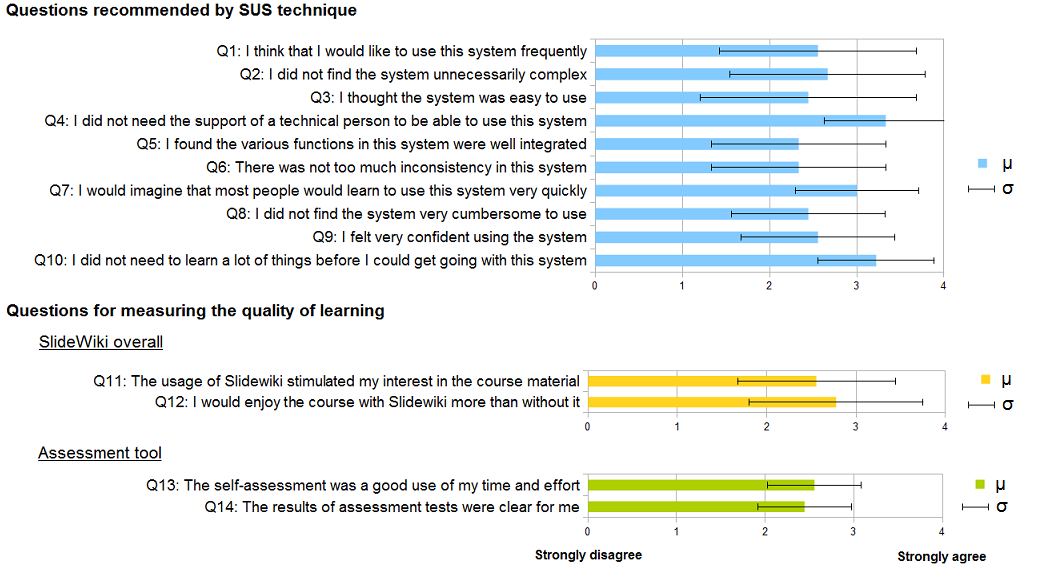
\includegraphics[width=\textwidth]{images/survey.png}
	\caption{Results of SlideWiki evaluation survey: mean $\mu$ and standard deviation $\sigma$.}
	\label{fig:survey}
\end{figure*}


In the first part of the questionnaire we included questions recommended by \emph{System Usability Scale} (SUS)~\cite{SUS2009} system to grade the usability of SlideWiki.
SUS is a standardized, simple, ten-item Likert scale-based questionnaire\footnote{\url{www.usabilitynet.org/trump/documents/Suschapt.doc}} giving a global view of subjective assessments of usability.
It yields a single number in the range of 0 to 100 which represents a composite measure of the overall usability of the system.
The results of our survey showed a mean usability score of \texttt{67.2} for SlideWiki which indicates a reasonable level of usability.

The second part of the questionnaire aimed to determine whether the SlideWiki helps to improve the quality of learning.
It consisted of four questions with five options from ``absolutely agree (1)''  to ``absolutely disagree (5)''.
The evaluation results for these two parts are presented in \autoref{fig:survey}.

Although the positive answers prevailed, we were not satisfied by the fact that for many questions a third of participants chose the neutral value.
The final part of the questionnaire helped us to understand the reasons.
We included here four open questions:
\small
\begin{enumerate}
	\item What did you like most about Slidewiki?
	\item What did you like least about Slidewiki?
	\item What can we do to improve the Slidewiki's usability?
	\item What features would you add to Slidewiki?
\end{enumerate}

Within the answers we found repeated complaints about several bugs, that interfered the working process.
We consider this fact to be the main reason of neutral and contradictory values.
However, we collected also positive opinions, especially about features and possibilities that SlideWiki allows.
Three of the recipients mentioned that they mostly liked that SlideWiki is easy to use, four of them noted, that they liked the idea of collaborative work and sharing the presentations itself.
Within the collected answers we also got important suggestions, which could be roughly divided into two groups:
\begin{itemize}
	\item Suggestions about desired improvements of existing features such as displaying the test results graphically, supporting more import formats, improving the SVG editor etc.
	\item Suggestions about totally new features, several of those were later implemented, e.g. translation, templates for presentation structure, etc.
\end{itemize}

The results of the initial evaluation were promising and we have continued the features development, trying to optimize the system performance and usability at the same time.

\subsubsection{Study at the University of Bonn}
After implementing the whole SlideWiki functionality we have conducted another study.
This time the goal was to have a detailed view at the problematic aspects of the implementation discovered through the previous study. 
Namely, questions of this survey were designed to evaluate the following three aspects:

\begin{enumerate}
\item Responsiveness of the SlideWiki website
\item Design and usability of the SlideWiki website
\item Functionality and awareness of the features and usage of the SlideWiki website
\end{enumerate}


The survey was divided into two parts.
The first part consisted of 17 multiple choice questions and the remaining 5 questions were left for comments and ideas.
We have received 23 anonymous responses out of 80 students registered for the “Semantic Data Web Technologies” course.

\begin{table}[!h]
\centering

\begin{tabularx}{0.9\columnwidth}{ l l }    
    \toprule
    
    \textbf{Question} & \textbf{Average} \\
    \midrule
    \rowcolor{LightGray}
    SlideWiki is easy to use. & 2.39 \\
	\midrule
	\rowcolor{LightGray}
    I find it easy to navigate through SlideWiki pages. & 2.3 \\
    \midrule
    \rowcolor{LightGray}
    SlideWiki provides a good user interface for learning slides. & 2.35 \\
    \midrule
    \rowcolor{LightGray}
    I find SlideWiki clear and well organized. & 2.57 \\
    \midrule
    \rowcolor{Gray}
    SlideWiki loads quickly on my computer (3-4 sec). & 2.39 \\
    \midrule
    \rowcolor{Gray}
    SlideWiki loads quickly on my mobile (3-4 sec). & 2.0 \\
    \midrule
    \rowcolor{Gray}
    I can immediately find response to my actions (mouse click). & 2.57 \\
    \midrule
    \rowcolor{LightGray}
    I can easily use SlideWiki on my mobile/tablet. & 2.17 \\
    \midrule
    \rowcolor{LightGray}
    I can use Slidewiki with different browsers. & 3.62 \\
    \rowcolor{Gray}
    \midrule
    I can easily download the slides. & 1.95 \\
    \midrule
    I found all the images, text, tables, etc. in the slides correctly rendered. & 2.32 \\
    \midrule
    \rowcolor{LightGray}
    I can easily navigate through the slide pages using the navigation tree. & 2.96 \\
    \midrule
    \rowcolor{LightGray}
    I had no problem finding the information I needed. & 2.48 \\
    \midrule
    I could find some bugs while using SlideWiki. & 3.78 \\
    \midrule
    I find all the links in the slides valid and active. & 3.38 \\
    \midrule
    I tried the Questions section of the slides and I found it helpful & 3.68 \\
    \midrule
    I tried the Discussion section of the slides and I found it helpful. & 2.95 \\
	\bottomrule
    \end{tabularx}
\caption{The multiple choice questions and the average of the answers (1 = strongly disagree and 5 = strongly agree), categorized by the cell colors: \colorbox{Gray}{dark-gray} referring to “Responsiveness of the website”, (2) \colorbox{LightGray}{light-gray} referring to “Design and usability” and (3) white referring to “Functionality and awareness of the website features and usage”}
\label{tab:bonn_evaluation}
\end{table}

The results of the study, as presented in ~\autoref{tab:bonn_evaluation}, proved our previous concerns about usability of the trial SlideWiki implementation, especially on mobile devices.
As well we have noticed even less satisfaction from SlideWiki performance than in the previous study, even though we have spent efforts to improve it.
We consider there are two main reasons for even lower SlideWiki user satisfaction we have found out through the second evaluation:
\begin{itemize}
\item Actual decrease in SlideWiki performance due to substantial growth of its database. Although the architecture of SlideWiki was proven to be scalable with increasing amount of content, the increased amount of users simultaneously working on the same presentation was not taken into account.
\item Increase of users expectations. During the development process new technological stacks and architectural patterns have appeared and spread widely, improving the possible performance of the systems with the similar scale. Thus, what have been considered to be relatively good performance at the beginning of development, has become not satisfying after the development has been finished.
\end{itemize}

However, the concepts underlying SlideWiki were still accepted by the users.
This was proven by open answers we have collected in the second part of the survey:
\paragraph{If you were to review your overall SlideWiki experience, what score would you give it out of 10?} 13 student gave it 5 and more, while 9 gave it less that 5.

\paragraph{What do you find most frustrating about SlideWiki?} Most of the comments concerned navigation, especially on mobile devices and slowness of loading.

\paragraph{If you could change one thing about SlideWiki what would it be and why?} Many students suggested improving the performance of loading slides.

\paragraph{What do you like best about SlideWiki?} As it can be seen from the~\autoref{tab:bonn_evaluation_open}, the students mentioned all main concepts we have based SlideWiki and the thesis except multilinguality:

\begin{table}[!h]
\centering

\begin{tabularx}{\columnwidth}{ll}    
    \toprule
    
    \textbf{Feature} & \textbf{\# of students} \\
    \midrule
    Collaboration on the educational material & 4 \\
    Different types of educational content, in particular, self-assessment items & 4\\
    Tree-structure of the content & 2 \\
    Accessibility of the content from everywhere & 2 \\
	\bottomrule
    \end{tabularx}
\caption{The most liked aspects of SlideWiki according to the final user evaluation}
\label{tab:bonn_evaluation_open}
\end{table}

\paragraph{How can we improve SlideWiki? Please tell us your ideas and suggestions?} Mostly students recommended changing layout (e.g. structure, minimalist design) and improving performance.

Based on the final evaluation results, we have concluded that the chosen architectural pattern and technological stack do not allow large-scale implementation of our concepts with satisfying performance.
We have analyzed the technical issues and have found  recently emerged technologies to solve them, as proposed in~\autoref{sec:slidewiki_new_generation}.
However, before the implementation of SlideWiki 2.0 we also needed to design the interface which considers all, even minor, UI issues indicated by the users.

\subsubsection{Single-user Observation}
In order to spot minor usability issues a single-user observation study~\cite{hasanov2015measuring} was conducted.
Three users, whose demographical data is described in ~\autoref{tab:single_user_demo}, were chosen.

\begin{table}[!h]
\centering

\begin{tabularx}{0.7\columnwidth}{l l l l l }    
    \toprule
    
    \textbf{\#} &\textbf{Gender} & \textbf{Age} & \textbf{Occupation} & \textbf{Computer Skills}\\
    \midrule
    
   1 & Female & 19 & Student Engineer & Good \\
	\midrule
	
    2 &  Male & 25 & IT helpdesk & Excellent \\
    \midrule
   
    3 &  Male & 22 & Economics Graduate & Average\\
    
	\bottomrule
    \end{tabularx}
\caption{Demographical data of users participating in the single-user observation study.}
\label{tab:single_user_demo}
\end{table}

In order to perform interaction with the Slidewiki, users were asked to complete the following sequence of actions:


1. Register on Slidewiki

2. Create a new empty presentation

3. Edit the presentation description

4. Add content to the first slide, using different text colors

5. Add an additional empty slide to your presentation

6. Add an image to the slide

7. Add an additional sub-deck to your presentation

8. Move the second slide you've created (with an image) to the new sub-deck

9. Change the title of the slide

10. Create a question to one of your slides

11. Download the presentation

12. Initiate the translation of the presentation into a different language 

13. Comment on the translated version

14. Change the slides theme and transitions of the translated version

15. Edit the presentation description of the translated version

16. Play the translated version

17. Find and open the deck "Open Educational habdbook"

18. Open a user page of any of the collaborators

19. Message him/her

20. Contact the website owners

21. Search using the search field for the presentation “Semantic Web Lectures”

22. Exam yourself in there.


After finishing all the stages, the users were asked to give comments and suggestions.
A screen recording tool was used in order to keep the video of the user interaction with the product for further exploit.
The found issues and possible solutions are summarized in ~\cite{hasanov2015measuring}. 
For example, while completing the task \#5 (\textit{Add an additional empty slide to your presentation}) all three users made at least 3 wrong actions and the fastest of them carried out the task within 47 seconds. 
In the current component implementation a user is supposed to complete the task by right-click on the deck title in the tree and choosing the necessary action from the drop-down list. 
However, this interface appeared to be not intuitive even for experienced users.
In order to solve the issue, we propose to add two small buttons for slide and deck adding, as depicted at ~\autoref{fig:deck_tree}.

\begin{figure}[ht!]
	\centering
		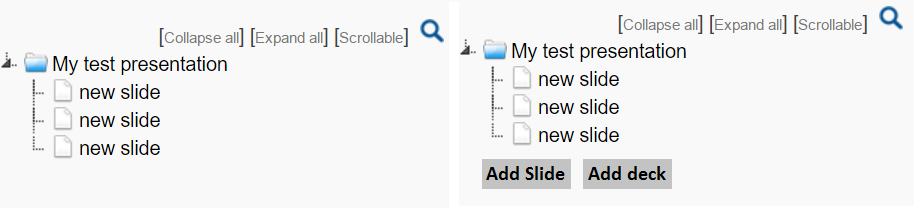
\includegraphics[width=\columnwidth]{images/deck_tree_mockup.png}
	\caption{The deck tree navigation component: current state (left) and proposed improvements (right)}
	\label{fig:deck_tree}
\end{figure}

Another common issue found is the presentation of search results.
The current state of the component is presented at ~\autoref{fig:search_current}.
All three users called their created deck using the word "test" and it was difficult to find the exact presentation within dozens of others.
As well, the tag cloud to filter the content is over-fulled, and at the same time does not have to be always visible for the users.
Our solution (see ~\autoref{fig:search_mockup}) for these issues is to (1) enhance the search functionality by adding additional scope for search by authors and tags, and (2) hide those advanced options until user needs them. 


\begin{figure}[ht!]
	\centering
		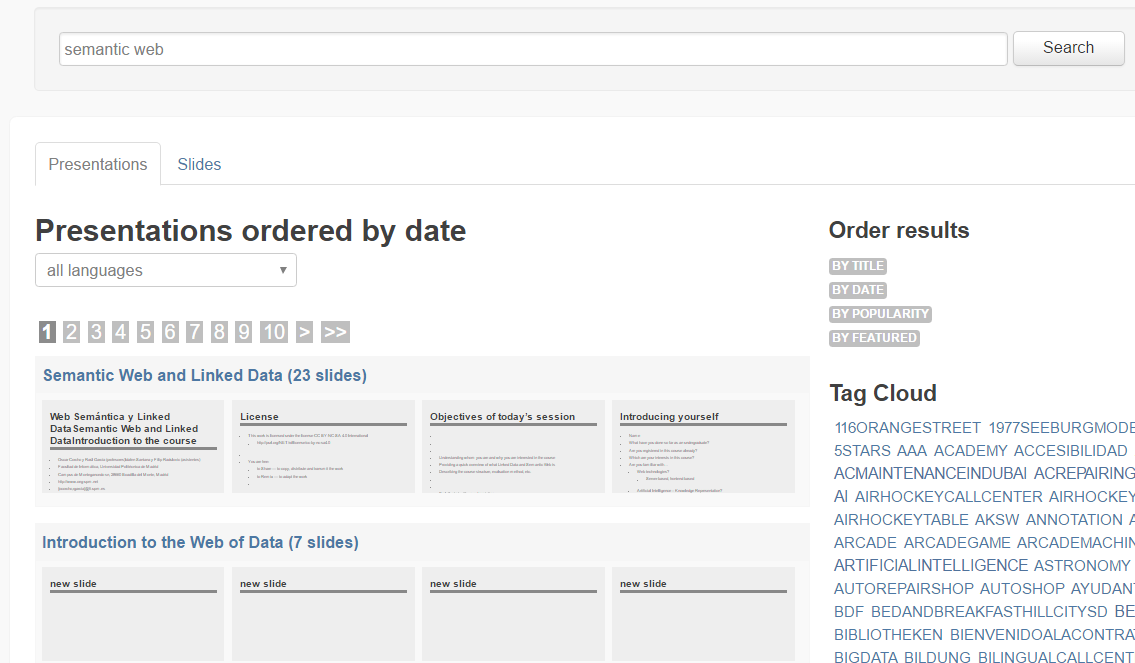
\includegraphics[width=\columnwidth]{images/search.png}
	\caption{The search component: current state}
	\label{fig:search_current}
\end{figure}

\begin{figure}[ht!]
	\centering
		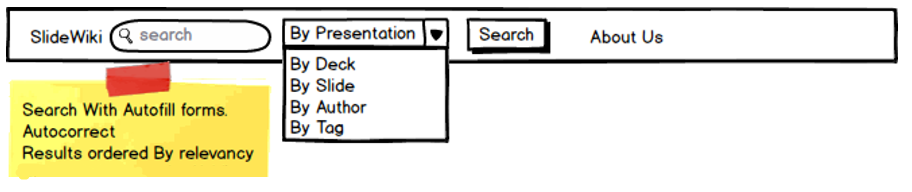
\includegraphics[width=\columnwidth]{images/search_mockup.png}
	\caption{The search component: proposed improvements}
	\label{fig:search_mockup}
\end{figure}



\subsection{Defined Issues of Current Implementation and Proposed Solutions}
\label{sec:slidewiki_new_generation}

Based on the evaluation results we can claim that the concepts behind SlideWiki are clear for users, they like the way of learning, storing and sharing of the presentations.
However the trial implementation has a number of issues. 

The initial design decision for using a relational approach for storing the data was made mainly due to the centralized MVC architecture pattern for data flow in the SlideWiki system. 
As well, immaturity of triple stores and NoSQL database technologies at the design time was another incentive to adopt relational approach.
The SlideWiki makes extensive use of the MVC where most of the complexity is handled on the backend-side (i.e. data layer) and views are mainly only serving content in different templates to users.
In such a centralized model, a relational model with support for join and aggregate queries was crucial.

However, although we have made additional effort to increase the platform performance, users continue to complain about its slowness.
Moreover, the emergence of mobile devices coupled with spreading wi-fi connection availability and quality led to the increased user expectations from web-based applications.
In response to these increased expectations appeared new architectures and technological stacks which comes in place of less-flexible MVC architecture backed by LAMP. 

Apart from the performance issue, as the number of developers, users and data on the platform started to grow, we faced new challenges with the relational data model and MVC architecture:

\begin{itemize}
\item{Evolving the data schema with emerging of the new requirements.} 
Using MySQL relational database, our application is constrained to a set of fixed schemata designed for the underlying tables.
When more developers joined the project and new requirements were identified, handling the changes and extending the underlying  schemata without affecting the related schemata became a cumbersome task.
In this situation, a schema-less design approach (e.g. existing document-based data models) to provide a dynamic schema vs. a predefined schema seemed to be crucial and more efficient.

\item{Horizontal scalability of platform as the number of data and users increase.}
As the number of data and users on our system increased, we noticed some performance issues in loading the pages.
Even though we implemented some caching mechanisms on the server, due to the dynamicity of SlideWiki environment, we still had to go for vertical scalability by increasing the CPU, RAM, SSD, etc, on our server which were quite expensive to sustain.
On the other hand, with the emergence of NoSQL databases which allow horizontal scalability, we could potentially be able to handle large traffic by just adding few more servers easily in our infrastructure.
In addition to that, MySQL database scaling was hard.
A single MySQL table performance would degrade when crossing the 5-10GB per table in SlideWiki.
In this case would need to partition and shard our database in a distributed way.

\item{Interoperability between the data model and front-end components.}
In the existing architecture, we have been using a complex object-relational mapping (ORM) layer that translates objects in code to relational tables.
Since JSON format is mainly used in our front-end to interact with data, translation to SQL and building the abstract data layer seems to be another burden to performance.
This adds a bottleneck to our system as the amount of nested data objects become large.
For example, to get a list of contributors of a deck, we need (1) to recursively go through the whole deck tree and get all its subdecks and slides, (2) to get contributors of each slide and (3) to aggregate the contributors.
Using existing NoSQL databases with native support for multilevel JSON could remove the complexity of ORM layer and increase the performance.

\item{Proving a high write time and high availability.}
Due to the wiki-based nature of SlideWiki, number of updates on data is very high.
Existing MySQL database with support for transactions in ACID model comes with the cost of lower write time and lower availability.
On the other hand, current NoSQL databases by default prefer high insert rate over transaction safety which would have a better fit in our SlideWiki requirements.

\item{Providing a Linked Data interface.}
One of the novel features in SlideWiki is providing highly structured e-learning content which could be queried and integrated with other educational material.
To achieve this goal, we are providing an RDF-based version of content on SlideWiki supported by a Linked Data interface which enables accessing and querying  data in a machine-readable format.
In the existing version, we used an RDB2RDF tool to convert the underlying relational model to a graph-based data model.
Exploiting a NoSQL database can facilitate this task to a great extent because of the underlying graph-based data model provided.
\end{itemize}

In order to solve the challenges, we propose to build the next generation of SlideWiki based on recently emergent MERN~\footnote{MongoDB-ExpressJS-ReactJS-NodeJS} technological stack in couple with microservice architecture.

\begin{figure*}[!ht]
\centering
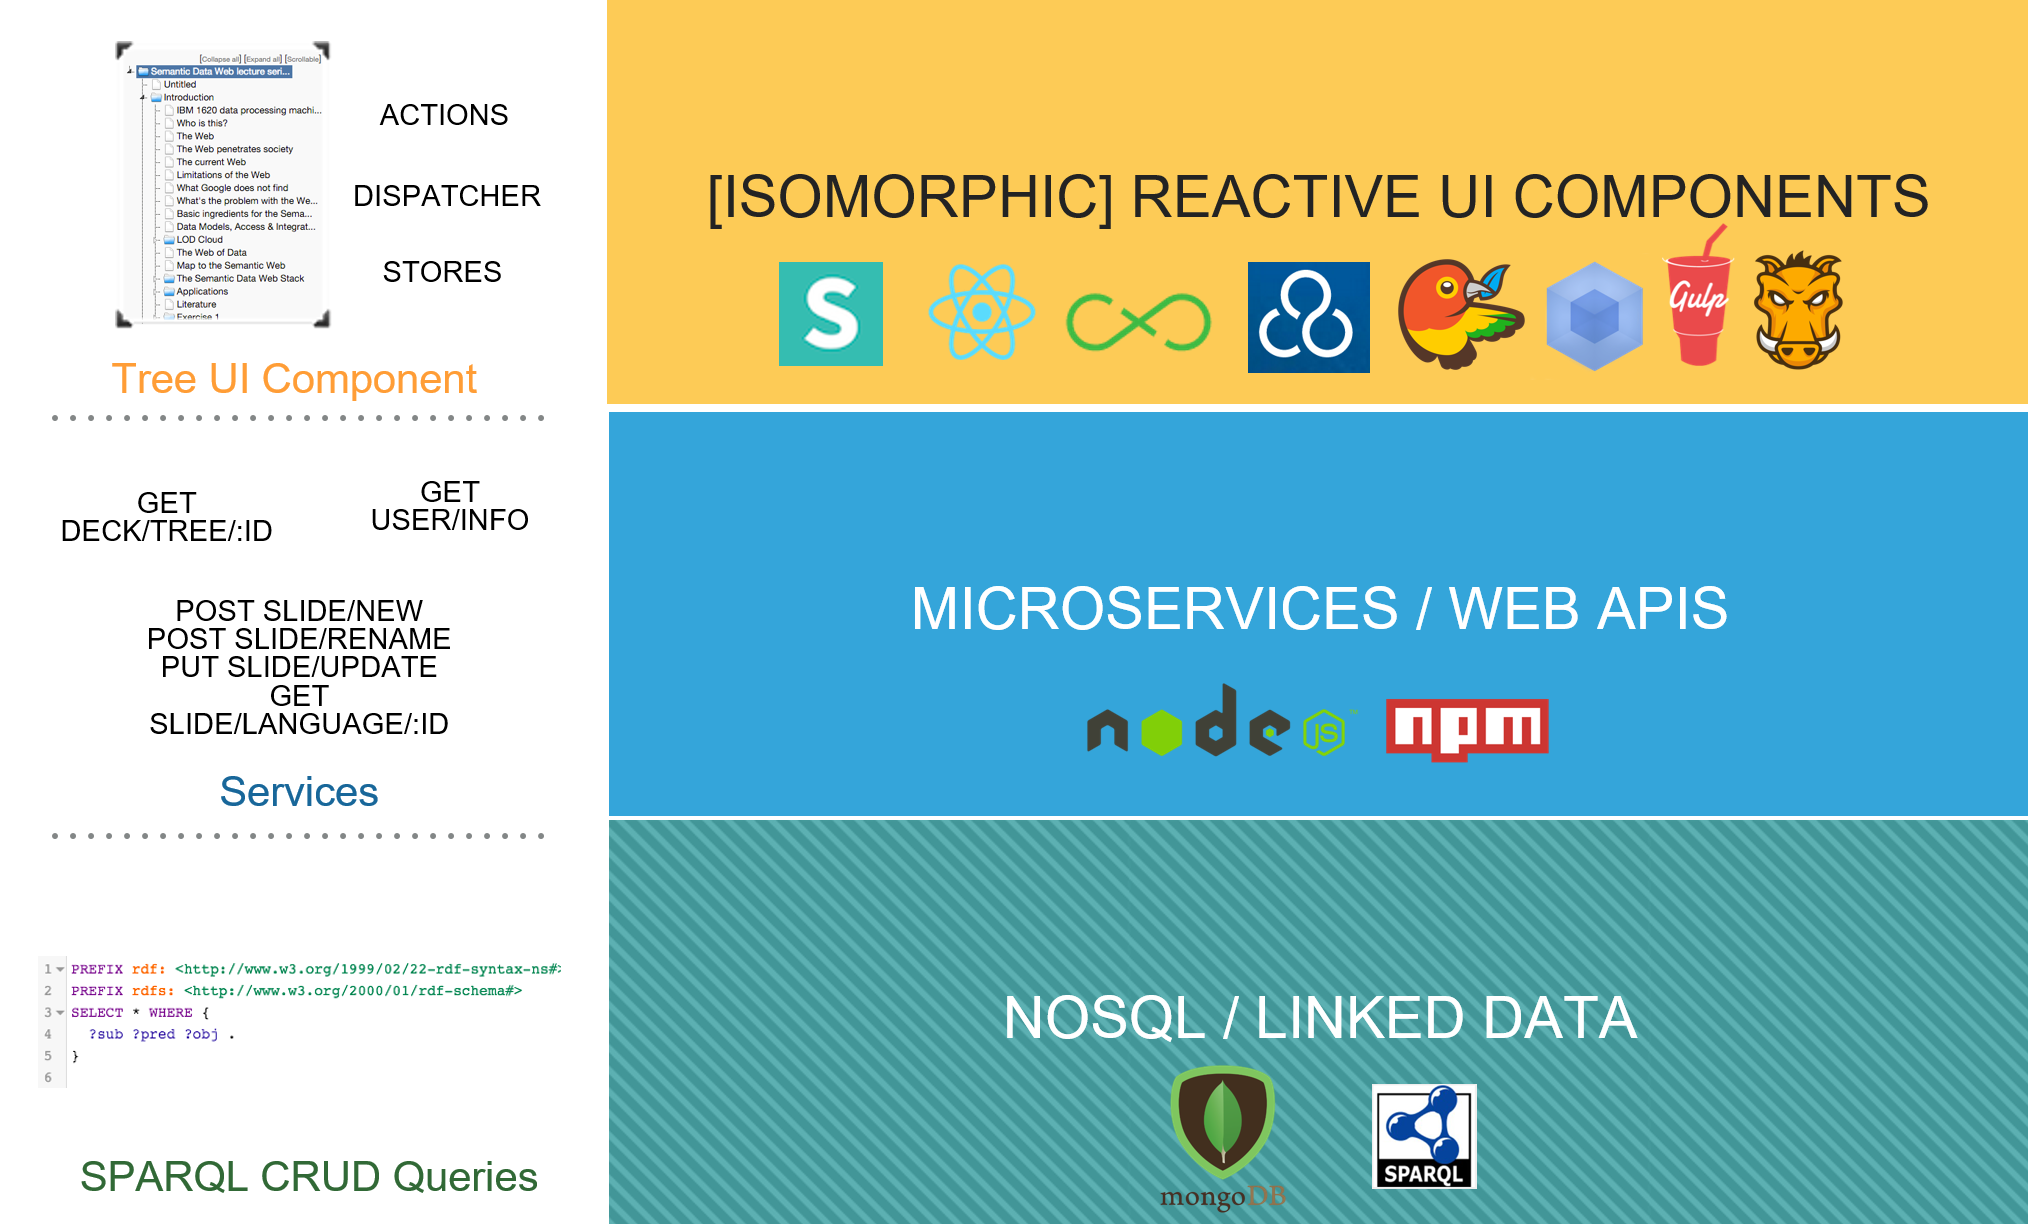
\includegraphics[width=1\textwidth]{Images/slidewiki2_architecture.png}
\caption{New Architecture of SlideWiki platform with an example usage (left side)}
\label{fig:slidewiki2_architecture}
\end{figure*}

As shown in ~\autoref{fig:slidewiki2_architecture}, the new architecture relies heavily on microservices which aim to distribute the complexity of our data layer among self-contained replicable Web services supporting horizontal scalability.
The main benefit of the microservice architecture is that it dramatically improves agility and velocity.
This is because when our system is correctly decomposed into a set of microservices and their dependent data schemas, we can develop and deploy each microservice independently and in parallel with the other services.
In order to enhance the interoperability, the proposed 3-tier architecture uses JSON as the communication language between user interface, services and data layer.
Apart from the improved performance, the proposed architecture facilitates the maintaining of the SlideWiki's code due to the component-based attitude of ReactJS.

%Since the initial SlideWiki design new approaches for enabling access to a web-site from various mobile devices have appeared.
%Contrary to the previous approaches, when web-sites usually had to provide separate interface for mobile device users, nowadays the responsive web design(RWD) approach is preferred.
%RWD aimes at crafting sites to provide an optimal viewing and interaction experience—easy reading and navigation with a minimum of resizing, panning, and scrolling across a wide range of devices (from desktop computer monitors to mobile phones).\cite{marcotte2013responsive}.
%A growing number of quality frameworks supporting RWD nowadays (for example, Semantic-UI~\footnote{\url{http://semantic-ui.com/}}) allow us to implement the responsive interface with a reasonable amount of efforts.
%
%Another issue is user interface clearness and quality of user documentation.
%Within the answers we have collected via user questionnaires were a few suggestions about features that were already implemented, but users were not aware of them.
%This encourages us to improve the documentation as well as to enhance the simplicity and clearness of the user interface.


%==============================================================================
\chapter{Collaboration on Self-assessment Items}
\label{chapter:self_assessment}
%============================================================================== 

The SlideWiki platform we have developed to evaluate our concepts allows to collaborate on different types of structured educational content? including self-assessment items.
The questions for self-assessment can be added to an individual slides by both teachers and students.
As slides are combined to a deck, the questions from the scope of slides are aggregated into a questionnaire assigned to the deck.
A deck with and assigned questionnaire can become a part of another deck, that allows us to implement module-based assessment of leaner performance.

In order the self assessment feature to work without teacher control, we have decided to limit the self-assessment items type to multiple-choice questions, where an item authors indicate which options are correct and which not. 
Advantages and disadvantages of a learning assessment based on multiple-choice questions (MCQs) are a long and widely discussed issue in the scientific community.
However, in practice this type of questions is very popular due to the possibility of automatic evaluation and scoring~\cite{Farthing1998}.
Consequently, an important research question is to exploit the strengths and mitigate the weaknesses of MCQs.

As well as some other systems (e.g. Moodle~\footnote{\url{https://moodle.org/}}) SlideWiki allows users to create MCQs with multiple correct options.
This type of questions we will call multiple-mark questions (MMQs), to distinguish them from the conventional MCQs, where there is always only one correct option.
Multiple-mark questions were already recommended by Cronbach~\cite{Cronbach}.
Other research~\cite{Ripkey1996,Pomplun1997,Hohensinn2011} considers MMQs to be more reliable, when compare them with conventional MCQs.

However, even though the advantages of MMQs are meanwhile widely accepted, up to our knowledge there are no balanced methods for scoring multiple-mark questions available to date.
One possible approach to score the MMQs is to use dichotomous scoring system. 
The dichotomous scoring awards the constant amount of points, when the question is answered correctly and zero points in a case of \textit{any} mistake.
However, the partial scoring is preferable to the dichotomous, especially in case of MMQs.~\cite{Ripkey1996,Jiao2012,Bauer2011,Ben-Simon1997} 

The second possible approach is to use the methods, developed for scoring the multiple true-false questions (MTFs).
However, despite the possibility to convert the MMQs into MTFs, the studies \cite{Cronbach,Dressel1953} show the differences between two formats.
Moreover, the researches mentioned above named the following disadvantages of MTF questions compared to MMQs:

\begin{itemize}
	\item The multiple true-false format "clouds" from the learners the possibility of marking several options as true.
	\item The level of reliability in multiple true-false questions is not equal for true and false answers.
	\item The multiple true-false format requires more resources to store the answers.
\end{itemize}

Another possible approach is to use penalties, similarly to the paper-based assessment where the teacher can analyze the student answers and decide how much points she deserves.
The method was proposed by Serlin~\cite{Serlin1978}.
For example, in Moodle a teacher has to determine what penalty applies for choosing each distractor.
However, this work is an additional, unpopular burden for content authors, since not required in paper-based tests.

Instead of asking the teacher, some systems calculate the penalties automatically. 
However, computer-based assessment opens additional possibilities to guess, for example choosing all options.
Often the scoring algorithms do not take into account such ways of guessing.
Consequently, we were facing the challenge to \textit{find a partial scoring method for MMQs, that was able to recognize and properly penalize guessing}.

\section{Terminology} %0.5
\label{sec:termin}

In the following we define the key concepts building the basis for our MMQ scoring method:

\textit{Dichotomous scoring} -- the concept of scoring the results, that allows users to get either the full amount of points or zero in a case of any mistake;

\textit{Partial scoring} -- the concept of scoring the results in a way that allows users to obtain some points for a question, which they answered only partially correct;

\textit{Difficulty} -- a difficulty weight of the question in the questionnaire in the interval $(0,1]$.
The difficulty can be determined automatically and dynamically based on prior scoring.
In our implementation, for example, difficulty is dynamically updated after one student provided an answer, according with the formula: 
	\[d' = \frac{incorr}{all}\]
In a case of dichotomous scoring, the values of $incorr$ and $all$ mean, respectively, the accumulated number of \textit{incorrect} and \textit{all} responses on the question by any user.
In a case of partial scoring, the definition of $incorr$ changes as follows:
	\[incorr = \sum_{i}1-d_{i}\]
where $i$ is a counter from 1 to the number of attempts for the question and
$D_{i}$ is the difficulty, that the question had at the moment, when the $i^{th}$-attempt was made.
After the difficulty is determined, it is scaled to the interval $(1,d_{max}]$, where $d_{max}$ is the maximal difficulty, that a question can have.
	\[d = f(d') = (d' *(d_{max}-1)+1 \]
The scaling is performed for better usability.
For example, $d_{max}$ can be set to 10 to obtain a difficulty level between 1 and 10.

\textit{Guessing level} -- the theoretical probability to guess the correct answer from the list of options.
In partial scoring, we determine the guessing level as the probability to obtain more than zero points.

\textit{Basic question points} -- an absolute value of points for the correctly checked options or the percentage of correctly checked options within all correct options.
Basic points = $f(d)$.

\textit{Penalty} -- the value, that should be deducted from the basic points due to the logic of the applied algorithm.
		In our approach we propose, that penalty should be only deducted, when user checks more options, than the number of correct ones.

\textit{Total question points} -- the amount of points for the question, gained by the user after the deduction of penalty.
		Total question score = $f(p,s)$.

\section{Existing Solutions}

There are several existing platforms, that use multiple-mark type of questions as well as several approaches to score them. 
We collected such approaches to describe, discuss and compare them.
Existing approaches for scoring the multiple-mark questions implement four base concepts.
In the paragraphs below we describe the basic ideas, advantages and disadvantages of these concepts.

\paragraph{Dichotomous scoring.}

This method is often used in paper-based questionnaires, where the good quality of questionnaires allows teacher to be more strict when score the results.
In the case choosing a wrong option indicates, that a student hopes to guess the correct response as she does not know the material behind the question well.
In e-based learning the quality of questionnaires is not perfect, especially in the systems with collaborative authoring.
That is why the dichotomous scoring can punish the learners for the teachers mistakes too much. 
As the aim of questionnaires is not only to score the results, but to catch the gaps of knowledge, the scoring of partially correct responses shows the actual knowledge of the student better.
Also, dichotomous scoring does not show the accurate progress of the student.
However, when dealing with multiple-mark questions dichotomous scoring almost excludes the possibility of guessing, that is why we use it as a standard of reference when evaluating our approach with real users.

\paragraph{Morgan algorithm.}
One of the historically first methods for scoring the MMQs was described in the 1979 by Morgan \cite{Morgan1979}.
In the accordance to the method, the scores are determined by the following algorithm:

\begin{enumerate}
    \item for each option chosen which the setter also considers correct, the student scores +1.
    \item for each option chosen which the setter considers to be incorrect, the student scores -1.
    \item for each option not chosen no score, positive or negative, is recorded regardless of whether the setter considers the response to be correct or incorrect.
\end{enumerate}

The algorithm can be improved by changing the constant 1 to dynamically determined amount of points:

\begin{enumerate}
    \item for each option chosen which the setter also considers correct, the student scores $+(p_{max}/n)$, where $n$ is a number of correct options
    \item for each option chosen which the setter considers to be incorrect, the student scores $-(p_{max}/k)$, where $k$ is a number of distractors.
\end{enumerate}

We use this improved algorithm for our experiments.
However, the experiments show a large dependence between number of options (correct and incorrect) and amount of penalty, that indicates the skewness of the method (see \autoref{subsec:experiment}).

\paragraph{MTF scoring.}

Multiple-mark questions can be scored with the approaches developed for multiple true-false items.
The base approach to score the MTF items is to determine, how close is the student response to the correct one.
Tsai~\cite{Tsai1993} evaluated six different implementations of the approach.
Later his findings were confirmed by Itten~\cite{Itten1997}.
Although both researches found partial crediting to be superior to dichotomous scoring in a case of MTFs, they do not consider any of the algorithms to be preferable. 
This fact allows us to use the most base of them for our experiments.

All the MTF scoring algorithms imply that any item has $n$ options and a fully correct response is awarded with full amount of points $p_{max}$.
If the user did not mark a correct option or marked a distractor, she is deducted with the penalty $s = p_{max}/n$ points.
Thus a student receives points for not-choosing a distractor as well as for choosing a correct option.
This point does not fit perfect to multiple-mark questions because of the differences between two types~\cite{Pomplun1997,Cronbach,Frisbie1992}.
Our experiments (see \autoref{subsec:experiment}) confirm the studies and show the skewness of the concept when deal with MMQs.
The main problem of the MTF scoring method, when applied to MMQs, is that a user obtains points, even if she did not chose any options. 
Although the problem can be solved by creating an additional rule,
the experiments show the further problems of the algorithm, when used for MMQ items. 


\paragraph{Ripkey algorithm.}

Ripkey~\cite{Ripkey1996} suggested a simple partial crediting algorithm, that we named by the author.
In the approach a fraction of one point depending on the total number of correct options is awarded for each correct option identified.
The approach assumes no point deduction for wrong choices, but items with more options chosen than allowed are awarded zero points.

The Ripkey's research showed promising results in a real-life evaluation.
However, later researches (e.g. Bauer~\cite{Bauer2011}) notice the limitations of the Ripkey's study.
The main issue in the Ripkey algorithm is the not well-balanced penalty.
Our experiments show that in many cases the algorithm penalizes so severely, that learners could consider it to be the dichotomous scoring. 
We had to improve the Ripkey's algorithm by adding the mathematical approach for evaluating the size of penalty.

\section{Mathematical model} %1.5
\label{subsec:math_model}

In our approach conventional MCQs are viewed as a particular case of multiple-mark questions, thus, the formulas can be applied to the tests mixed of MCQs and MMQs.
As the scoring of conventional MCQs is a trivial task, we do not consider such type of questions in our experiments.

The task to find the scoring method can be divided into two steps:

\begin{enumerate}
	\item Find a method to determine points for the correctly marked options.
	\item Find a method to determine the penalty for the incorrectly marked options.
\end{enumerate}

For the first part a reasonable approach was proposed by Ripkey~\cite{Ripkey1996}, as discussed above.
Our research aims to provide a method for the second part (determining penalties).
We have developed a general approach and a mathematical model, that takes into account the most common ways of guessing and behaves balanced at the same time.

Our concept is based on the assumption, that scoring can be based on the guessing level of the question.
Each question is associated with a difficulty to guess a (partially) correct answer.
To accommodate the difficulty level of guessing in the scoring method, we propose to determine the penalty only when a student marks more options, than the actual number of correct ones.
Thus, when a student marks all possible options, she increases the guessing level up to 1. 
In this case the student should obtain either the full amount of points (if all the options are considered to be correct by the teacher), or zero, if the question has at least one distractor. 
However, if a student did not mark any option, the score should be always zero, as we assume that all the questions have at least one correct option.
Thus, the task is to find the correctness percentage of the response and decrease it with a penalty, if the guessing level was artificially increased by marking too many options.

Questions have the native level of guessing, and we propose to deduct the penalty only if after the student's response the guessing level increases.
In other words, we determine the penalty only when a student marks more options, than the number of correct ones.



In this section we present the mathematical model as well as an algorithm, that can be used for its implementation. 

\subsubsection{Assumptions and restrictions}
\label{subsec:restrictions}

We propose to use our approach only in systems, that comply with the following requirements for assessment items:

\begin{itemize}
  \item all the item's options have the same weight;
  \item there is at least one correct option;
  \item there are no options excluding all other (e.g. "all above are correct")
\end{itemize}
\begin{figure}[h!]
	\centering
		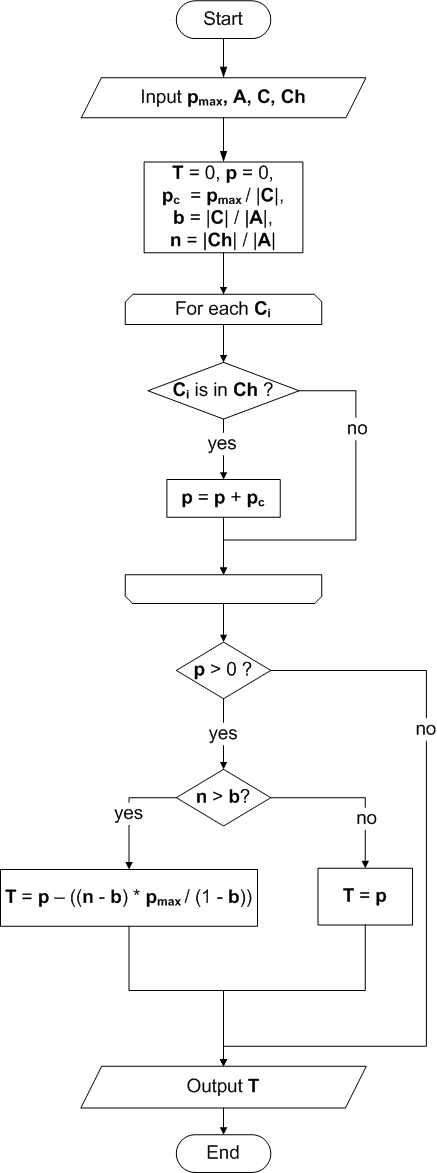
\includegraphics[width=.47\columnwidth]{images/algorithm.jpg}
	\caption{Flow chart of the Balanced scoring algorithm.}
	\label{fig:algorithm}
\end{figure}

\subsubsection{Scoring the basic points}

To score the basic points we use the approach, described by Ripkey. 
Below we present it mathematically in accordance with the following designations:

\begin{itemize}
    \item $d \in \mathbb{R} , d \in (1..d_{max}]$ -- difficulty of the current question, for our experiments we set $d_{max} = 5$ 
    \item $C \subseteq A$ -- set of the \textit{correct} options $c_i$ for the current question, where $A$ -- set of the options $a_j$ for the current question,
    \item $c_{max} = |C| , c_{max} \in \mathbb{N}$ -- number of \textit{correct} options for the current question
    \item $C_{ch}$ -- set of the \textit{correctly checked} options
    \item $c_{ch} = |C_{ch}| , c_{ch} \in \mathbb{N} , c_{ch} \in [0,c_{max}]$ -- number of \textit{correctly checked} options for the current question
    \item $p_{max} = f(d) = d*K_{points}$ -- maximal possible points for the current question, in our system we set $K_{points} = 1$
    \item $p_c$ -- points for the correctly checked option $c$. 
    As we assume all the correct options have the equal weight, 
    \[\forall c \in C_{ch} \vert p_c = \frac{p_{max}}{c_{max}}\]
    \item $p \in \mathbb{R} \wedge p \in [0,p_{max}]$ -- the basic points for the current question,
    \[p = \sum_{c \in C_{ch}}{p_c} \Rightarrow \]

   \[p = \sum_{c \in C_{ch}}{\frac{p_{max}}{c_{max}}} = \frac{p_{max}}  {c_{max}}*c_{ch} = p_c*c_{ch}\]
\end{itemize}

\subsubsection{Scoring the penalty}

Below we present our approach for scoring the penalty.
We use the following designations:

\begin{itemize}
    \item $a_{max} \in \mathbb{N} , a_{max} = |A|$ -- number of options $a \in A$
    \item $Ch \subseteq A$ -- set of \textit{checked} options
    \item $ch = |Ch| , ch \in \mathbb{N} , ch \in [0,a_{max}]$ -- number of checked options for the current question
    \item $b \in \mathbb{R} , b \in [0,1]$ -- basic level of guessing for the current question, 
    \[b = \frac{c_{max}}{a_{max}}\]
    \item $n \in \mathbb{R} , n \in [b,1]$ -- measure, that shows the possibility, that user tries to guess the correct response by choosing too much options; we do not evaluate it in the cases, when $n <= b$,
   \[n = \frac{ch}{a_{max}}\]
    \item $s$ -- penalty for the guessing,
    \[s = n-b \Rightarrow s \in [0,1-b]\]
    \item $s_k \in [0,p_{max}]$ -- the penalty, mapped to the maximal possible points.
\end{itemize}

A mapping function is calculated as follows:
\[f : s_k \rightarrow s\]
Given, $s_k \in [0,p_{max}]$ and $s \in [0,1-b]$, then 
\[f : s_k \rightarrow s = f : [0 , {1-b}] \rightarrow [0,p_{max}] \Rightarrow\]
\[s_k = f(s) = s*\frac{p_{max}}{1-b} = (n-b)*\frac{p_{max}}{1-b}\]

\subsubsection{Scoring the total question score}

The absolute score for the question is trivially determined as
\[T = f(p,s_k) = p-s_k \]
The percentage representation of the total score is determined as follows:
\[T_\% = \frac{p - s_k}{p_{max}}*100\%\]


\section{Synthetic experiments}
\label{subsec:experiment}

In the subsection we describe our experiments with synthetic data and compare the behavior of different methods.
For shorter presentation, we use the following reductions:

\begin{itemize}
  \item{Dich.} -- dichotomous scoring;
  \item{Balanced} -- the proposed balanced scoring method
\end{itemize}

We consider all questions to have the difficulty $d = 1$, then the maximal possible points $p_{max} = 1$ as well.

\begin{table}[h!]
	\centering
%	\renewcommand{\tabcolsep}{0.15cm}
%	\renewcommand{\arraystretch}{1.3}
	\begin{tabularx}{0.5\columnwidth}{c c c c c}  
	\toprule  
    \multicolumn{5}{c}{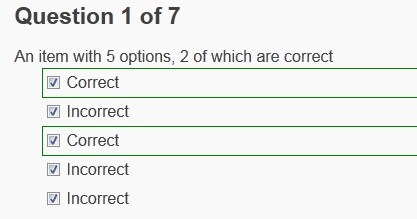
\includegraphics[width=0.5\columnwidth]{images/case1.jpg}}\\
    \midrule
    \textbf{Dich.}&\textbf{MTF}&\textbf{Morgan}&\textbf{Ripkey}&\textbf{Balanced}\\
	\midrule
    0&0.4&0&0&0\\
	\bottomrule
    \end{tabularx}
	\caption{Comparison of the proposed approach with other existing approaches}
	\label{tab:case 1}
\end{table}

\begin{example}[Case: 5 options, 2 correct, 5 marked]
In the case a student chose all the options and should obtain zero points. 
However, we see that MTF method does not recognize this type of guessing and considers the questions to be answered partially correct, awarding the points for two correct options, that were marked.
\end{example}

\begin{table}[h!]
	\centering
%	\renewcommand{\tabcolsep}{0.15cm}
%	\renewcommand{\arraystretch}{1.3}
	\begin{tabularx}{0.5\columnwidth}{c c c c c} 
	\toprule  
    \multicolumn{5}{c}{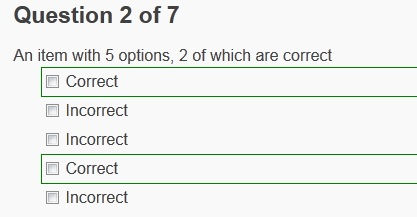
\includegraphics[width=0.5\columnwidth]{images/case2.jpg}}\\
    \midrule
    \textbf{Dich.}&\textbf{MTF}&\textbf{Morgan}&\textbf{Ripkey}&\textbf{Balanced}\\
	\midrule
    0&0.6&0&0&0\\
	\bottomrule
    \end{tabularx}
	\caption{Comparison of the proposed approach with other existing approaches}
	\label{tab:case 2}
\end{table}

\begin{example}[Case: 5 options, 2 correct, 0 marked]
The situation is opposite to the previous: in the case a student chose none of the options. 
As we assume that question must have at least one correct option, in  case of not choosing any options a student also should obtain zero points.
However, we see that MTF method awards the points for three distractors, that were not marked.
Although the situation is absurd, we faced it within real learning platforms, for example within several on-line courses of the Stanford University~\footnote{http://online.stanford.edu/courses}.
\end{example}

Two examples below are trivial and the problem could be solved by adding the rules. 
However, the MTF scoring also suffers from skewness, when applied to MMQs, as it is shown below.

\begin{table}[h!]
	\centering
%	\renewcommand{\tabcolsep}{0.15cm}
%	\renewcommand{\arraystretch}{1.3}
	\begin{tabularx}{0.5\columnwidth}{c c c c c} 
	\toprule  
    \multicolumn{5}{c}{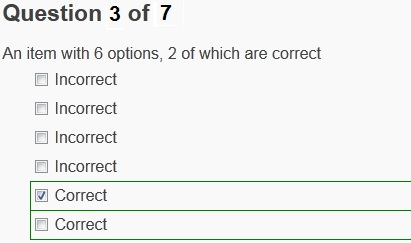
\includegraphics[width=0.5\columnwidth]{images/case3.jpg}}\\
    \midrule
    \textbf{Dich.}&\textbf{MTF}&\textbf{Morgan}&\textbf{Ripkey}&\textbf{Balanced}\\
	\midrule
    0&0.83&0.5&0.5&0.5\\
	\bottomrule
    \end{tabularx}
	\caption{Comparison of the proposed approach with other existing approaches}
	\label{tab:case 3}
\end{table}

\begin{example}[Case: 6 options, 2 correct, 1 correct marked]
This case proves, that the MTF method has a dependency from a number of correct and incorrect options. 
Thus, in a case of 6 options two of which are correct, a student is awarded 0.833 points for choosing only one correct option.
In a case of 5 options two of which are correct, she would be awarded 0.80 points for the same.
Moreover, if she choose only one incorrect option in a case of 6 alternatives, she obtains 0.5 points; in a case of 5 options she will be awarded 0.4 for the same.
\end{example}

Thus, our experiments prove, that multiple-mark questions can not be scored properly with the algorithms, developed for multiple true-false items.
Moreover, a teacher should be careful when creating multiple true-false questions and create them in such a manner, that not-choosing a distractor deserves awarding.
However, the MTF scoring is the only existing approach of partial scoring that can be used in a case, when a question does not have any correct options.

\begin{table}[h!]
	\centering
%	\renewcommand{\tabcolsep}{0.15cm}
%	\renewcommand{\arraystretch}{1.3}
	\begin{tabularx}{0.5\columnwidth}{c c c c c} 
	\toprule 
    \multicolumn{5}{c}{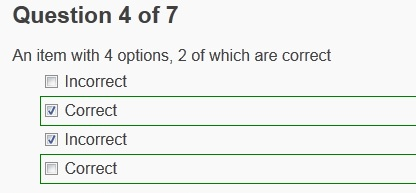
\includegraphics[width=0.5\columnwidth]{images/case4.jpg}}\\
    \midrule
    \textbf{Dich.}&\textbf{MTF}&\textbf{Morgan}&\textbf{Ripkey}&\textbf{Balanced}\\
	\midrule
    0&0.5&0&0.5&0.5\\
	\bottomrule
    \end{tabularx}
	\caption{Comparison of the proposed approach with other existing approaches}
	\label{tab:case 4}
\end{table}

\begin{example}[Case: 4 options, 2 correct, 1 correct and 1 incorrect marked]
This case illustrates the issues of using the Morgan algorithm.
The Morgan algorithm deducts penalties for choosing the incorrect option, as well as the proposed approach.
There are two main issues:

\begin{itemize}
  \item Does the response deserve penalty?
  \item If deserves, how big the penalty should be?
\end{itemize}

In that case we are facing the situation, that penalty has the same size, as the basic points, and the student is awarded zero.
We consider the penalty to be needlessly high, especially because the penalty depends on the number of incorrect options.
Thus, if the question has 3 incorrect options, choosing one of them would be fined on 0.33, and in case of 2 incorrect options, the penalty is 0.5.
After recognizing behavior of the algorithm, students will mark only the options, they are sure in, because choosing an incorrect one may cost them a full amount of points, they collected with correct options.
\end{example}

The next two examples show mainly the differences between the proposed approach and Ripkey algorithm.
Namely, we show the situations, when Ripkey algorithm awards zero points, while we consider that it should award more. 

\begin{table}[h!]
	\centering
%	\renewcommand{\tabcolsep}{0.15cm}
%	\renewcommand{\arraystretch}{1.3}
	\begin{tabularx}{0.5\columnwidth}{c c c c c} 
	\toprule  
    \multicolumn{5}{c}{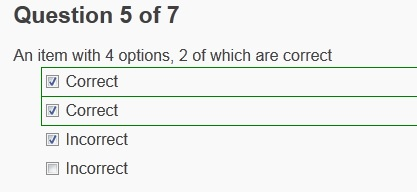
\includegraphics[width=0.5\columnwidth]{images/case5.jpg}}\\
    \midrule
    \textbf{Dich.}&\textbf{MTF}&\textbf{Morgan}&\textbf{Ripkey}&\textbf{Balanced}\\
	\midrule
    0&0.75&0.5&0&0.5\\
	\bottomrule
    \end{tabularx}
	\caption{Comparison of the proposed approach with other existing approaches}
	\label{tab:case 5}
\end{table}

\begin{example}[Case: 4 options, 2 correct, 2 correct and 1 incorrect marked]
In this case the student chose more options, than the number of correct ones, and according to the Ripkey, the answer should be awarded zero.
Our claim is, that until the student have not chosen all the options, she could have some points.
However, choosing three of four options could mean a try of guessing.
Although in this case the student gets the full amount of \textit{basic} points, she is fined on a half of them.
\end{example}

\begin{table}[h!]
	\centering
%	\renewcommand{\tabcolsep}{0.15cm}
%	\renewcommand{\arraystretch}{1.3}
	\begin{tabularx}{0.5\columnwidth}{c c c c c} 
	\toprule  
    \multicolumn{5}{c}{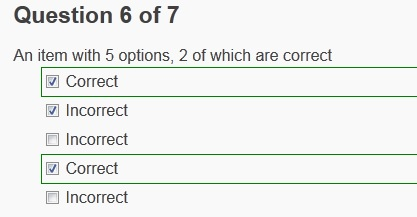
\includegraphics[width=0.5\columnwidth]{images/case6.jpg}}\\
    \midrule
    \textbf{Dich.}&\textbf{MTF}&\textbf{Morgan}&\textbf{Ripkey}&\textbf{Balanced}\\
	\midrule
    0&0.8&0.67&0&0.67\\
	\bottomrule
    \end{tabularx}
	\caption{Comparison of the proposed approach with other existing approaches}
	\label{tab:case 6}
\end{table}

\begin{example}[Case: 5 options, 2 correct, 2 correct and 1 incorrect marked]
The example shows the disadvantage of the Ripkey algorithm more clear.
It is not clear for the student, why she was awarded zero points, as she did not try to guess and answered partially correct.
\end{example}

\begin{table}[h!]
	\centering
	\begin{tabularx}{0.5\columnwidth}{c c c c c}    
    \toprule
    \multicolumn{5}{c}{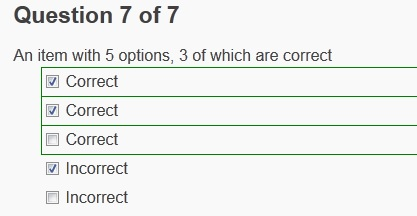
\includegraphics[width=0.5\columnwidth]{images/case7.jpg}}\\
    \midrule
    \textbf{Dich.}&\textbf{MTF}&\textbf{Morgan}&\textbf{Ripkey}&\textbf{Balanced}\\
	\midrule
    0&0.6&0.17&0.67&0.67\\
	\bottomrule
    \end{tabularx}
	\caption{Comparison of the proposed approach with other existing approaches}
	\label{tab:case 7}
\end{table}

\begin{example}[Case: 5 options, 3 correct, 2 correct and 1 incorrect marked]
In that case balanced scoring and Ripkey algorithms behave the same, as none of them deducts a penalty.
\end{example}


\section{Conclusions}
\label{sec:conclusions}
\todo{expand conclusions to the thesis topic}
During the research we have evaluated the existing approaches for scoring the multiple-mark questions and proposed a new one.
The proposed approach has a list of restrictions, however it has advantages when compare with the discussed approaches.
One of the main advantages is its clearness for the students, that was proven by a user evaluation (see~\autoref{sec:impl_e-learning}).
Also, our approach is based on the mathematical model, it does not suffer from the skewness, as it has the same formula for all cases.
At the same time, the proposed approach recognizes the attempts to guess the correct answer, for example choosing all the possible options.
When compare with the existing approaches, the advantages of the proposed algorithm could be summarized as follows:

\begin{itemize}
  \item The approach allows to score both multiple-mark and conventional multiple-choice questions.
  \item The approach is based on the partial scoring concept.
  \item The algorithm can be easily implemented, it is pure mathematical.
  \item The score does not highly depend on the amount of correct and incorrect options.
  \item The value of the penalty is in balance with the possibility, that the student is trying to guess.
  \item Due to the balance, the results are clear for the students.  
\end{itemize}

However, we suppose our algorithm to be optional together with other discussed approaches.
This is due to the fact, that users create questions in their own manner and should be able to choose an appropriate method to score the results.
Also, the different situations require different levels of 	
severity, and the proposed approach might be too lenient.



%==============================================================================
\chapter{Discussion and Conclusion}
\label{chapter:conclusion}
%==============================================================================

A major obstacle of increasing the efficiency, effectiveness and quality of education in Europe is the lack of widely available, accessible, multilingual, timely, engaging and high-quality educational material (i.e. OpenCourseWare).
The creation and maintenance of comprehensive OCW is tedious, time-consuming and expensive, with the effect that often courseware employed by teachers, instructors and professors is incomplete, outdated, dull and inaccessible to those with disabilities. 
Universities create much of the world’s intellectual capital and are eager to share this knowledge beyond the walls of the academy and to grant access to education for everyone.
Unfortunately, cash-strapped institutions and schools have found it difficult to scale the significant organizational, technical, and cost barriers to distribution of rich OpenCourseWare plus also support interoperability and fully satisfy accessibility demands.

In the current thesis we aimed to contribute to the problem by providing a complex solution for the collaborative OCW development.
In order to do so, we have firstly defined the major technological and conceptual gaps.
Then we have developed missing concepts and evaluated them with an innovative SlideWiki platform.

The results of systematic literature study showed us the lack of conceptual and technological solutions for features supporting the collaborative OCW authoring.
Namely, the issues of content localization, remixing and repurposing, as well as user engagement and coordination were not discussed enough in the previously existing research.
In the scope of the thesis we have provided our own solutions to these issues:
\begin{itemize}
\item In order to engage and coordinate collaborators we have developed a CrowdLearn concept, that applies social networking techniques to the structured content development.
\item To facilitate the content reuse and re-purpose we have developed the WikiApp data model, that presents the content as a sequence of content pieces, each of which can be operated and reused independently.
\item In order to enable a fully-featured collaboration on multilingual educational content we have developed the CoSMEC concept, which allows synchronization and co-evolution of the content between its versions in different languages.
\end{itemize}

We have implemented and evaluated the developed concepts within a mid-size proof-of-concept application SlideWiki.
The application deals with two types of structured OERs: slide sets and self-assessment item sets attached to the slides.
Both content types can be operated collaboratively, with enchanted possibilities for cross-lingual reuse and repurpose.  
The results of the evaluation showed us that the developed concepts do work together with a synergistic effect, even though the implementation lacked technical maturity.
The SlideWiki platform 

Although many of the techniques employed by SlideWiki (e.g. crowdsourcing, semi-automatic translation, semantic structuring, cloud-computing) are well-known, their combination and tailored application for OpenCourseWare authoring is novel and innovative:
\begin{itemize}
\item The \textbf{crowdsourced creation of OpenCourseWare} as performed with SlideWiki applies concepts such as fine-grained branching and merging to learning content (remixing and repurposing), which are already established in other fields such as software development (Github) or content management (Wikis).
\item The \textbf{semantic structuring} of the content in SlideWiki allows novel reuse and remixing scenarios and also facilitates the accessible, inclusive and ubiquitous representation of content stored in the system.
\item The \textbf{semi-automatic multilingual authoring} enables the sharing of learning content translation and maintenance effort between many community members. Since all content is versioned and semantically structured, it is trivial to (automatically) translate content and to keep track of changes in various multilingual versions of the same content object.
\item The \textbf{intertwining of the technological advances and accompanying community building}, fostering and cross-fertilization functions helps establishing a socio-technological ecosystem, which makes the SlideWiki service an innovative, world-wide used educational content facility.
\end{itemize}

The innovative SlideWiki functionality is beneficial for different types of users, including:
\begin{itemize}
\item \textbf{Educators, Lecturers and Teachers} can significantly increase the user base by making the content accessible to a worldwide audience, obtain translations of their high-quality content in many different languages.
They can engage students in contributing to and discussing the courseware and easily create (self-)assessment tests for students.
Peer-educators can be involved in improving and maintaining the quality and attractiveness of the learning content.
Ultimately sharing and contributing to qualitative content will increase the educator’s reputation in the community.
\item\textbf{ Students and Learners} obtain access to an unprecedented repository of freely available, multilingual and high-quality OpenCourseWare.
They can view rich-learning content right in a browser, discuss particular content (e.g. a slide or question) with other students and instructors and contribute additional content, improvements and feedback.
They are empowered to assess their learning progress using the questionnaires attached to presentations.
\item \textbf{Schools and Universities} can make courseware easily accessible (since each presentation and slide has its own URL), leverage the wisdom of educator crowd, which can collaborate efficiently in creating rich educational content, make the e-learning content produced in the organization really re-usable and re-mixable as well as increase the reputation of the school by sharing quality content.
\item For \textbf{Companies} presentations are a crucial element of the corporate knowledge exchange.
SlideWiki can help to make the knowledge available in a company easily accessible to everyone (in the company), engage employees in sharing and reusing knowledge available in presentations.
In addition to the public SlideWiki portal companies can install and run a SlideWiki instance inside their corporate Intranet with access control.
\end{itemize}

Due to these innovations SlideWiki won the OpenCourseWare Consortium’s Excellence Award in 2014 (see~\autoref{fig:ocw_global_award}) and is already used by hundreds of educators and thousands of learners.
Several hundred comprehensive course materials are available on SlideWiki in dozens of languages.
The maturity and innovative nature of the concepts behind SlideWiki allows us to claim that the gaps found in the domain are filled with the SlideWiki platform, as shown at~\autoref{fig:slidewiki_place_2}.


\begin{figure}
\centering
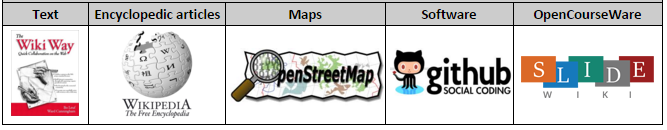
\includegraphics[width=\columnwidth]{images/filled_spot.png}
\caption{Collaborative authoring platforms in various domains}
\label{fig:slidewiki_place_2}
\end{figure}

In order to extend the trial SlideWiki implementation to a large scale we will further develop and enhance the platform in scope of EU funded project.
In order to turn SlideWiki into a large-scale European platform the consortium of 17 European educational and research organizations will collaborate on all aspects of the development, management and evaluation. 
The consortium along with its European and international partner organizations is committed to support and sustain SlideWiki.
As well, it aims to rise the community awareness for an easy-to-use and barrier-free possibility for the creation of Open Educational content that can be shared, mixed and re-edited across platforms and device borders.

\begin{figure}
\centering
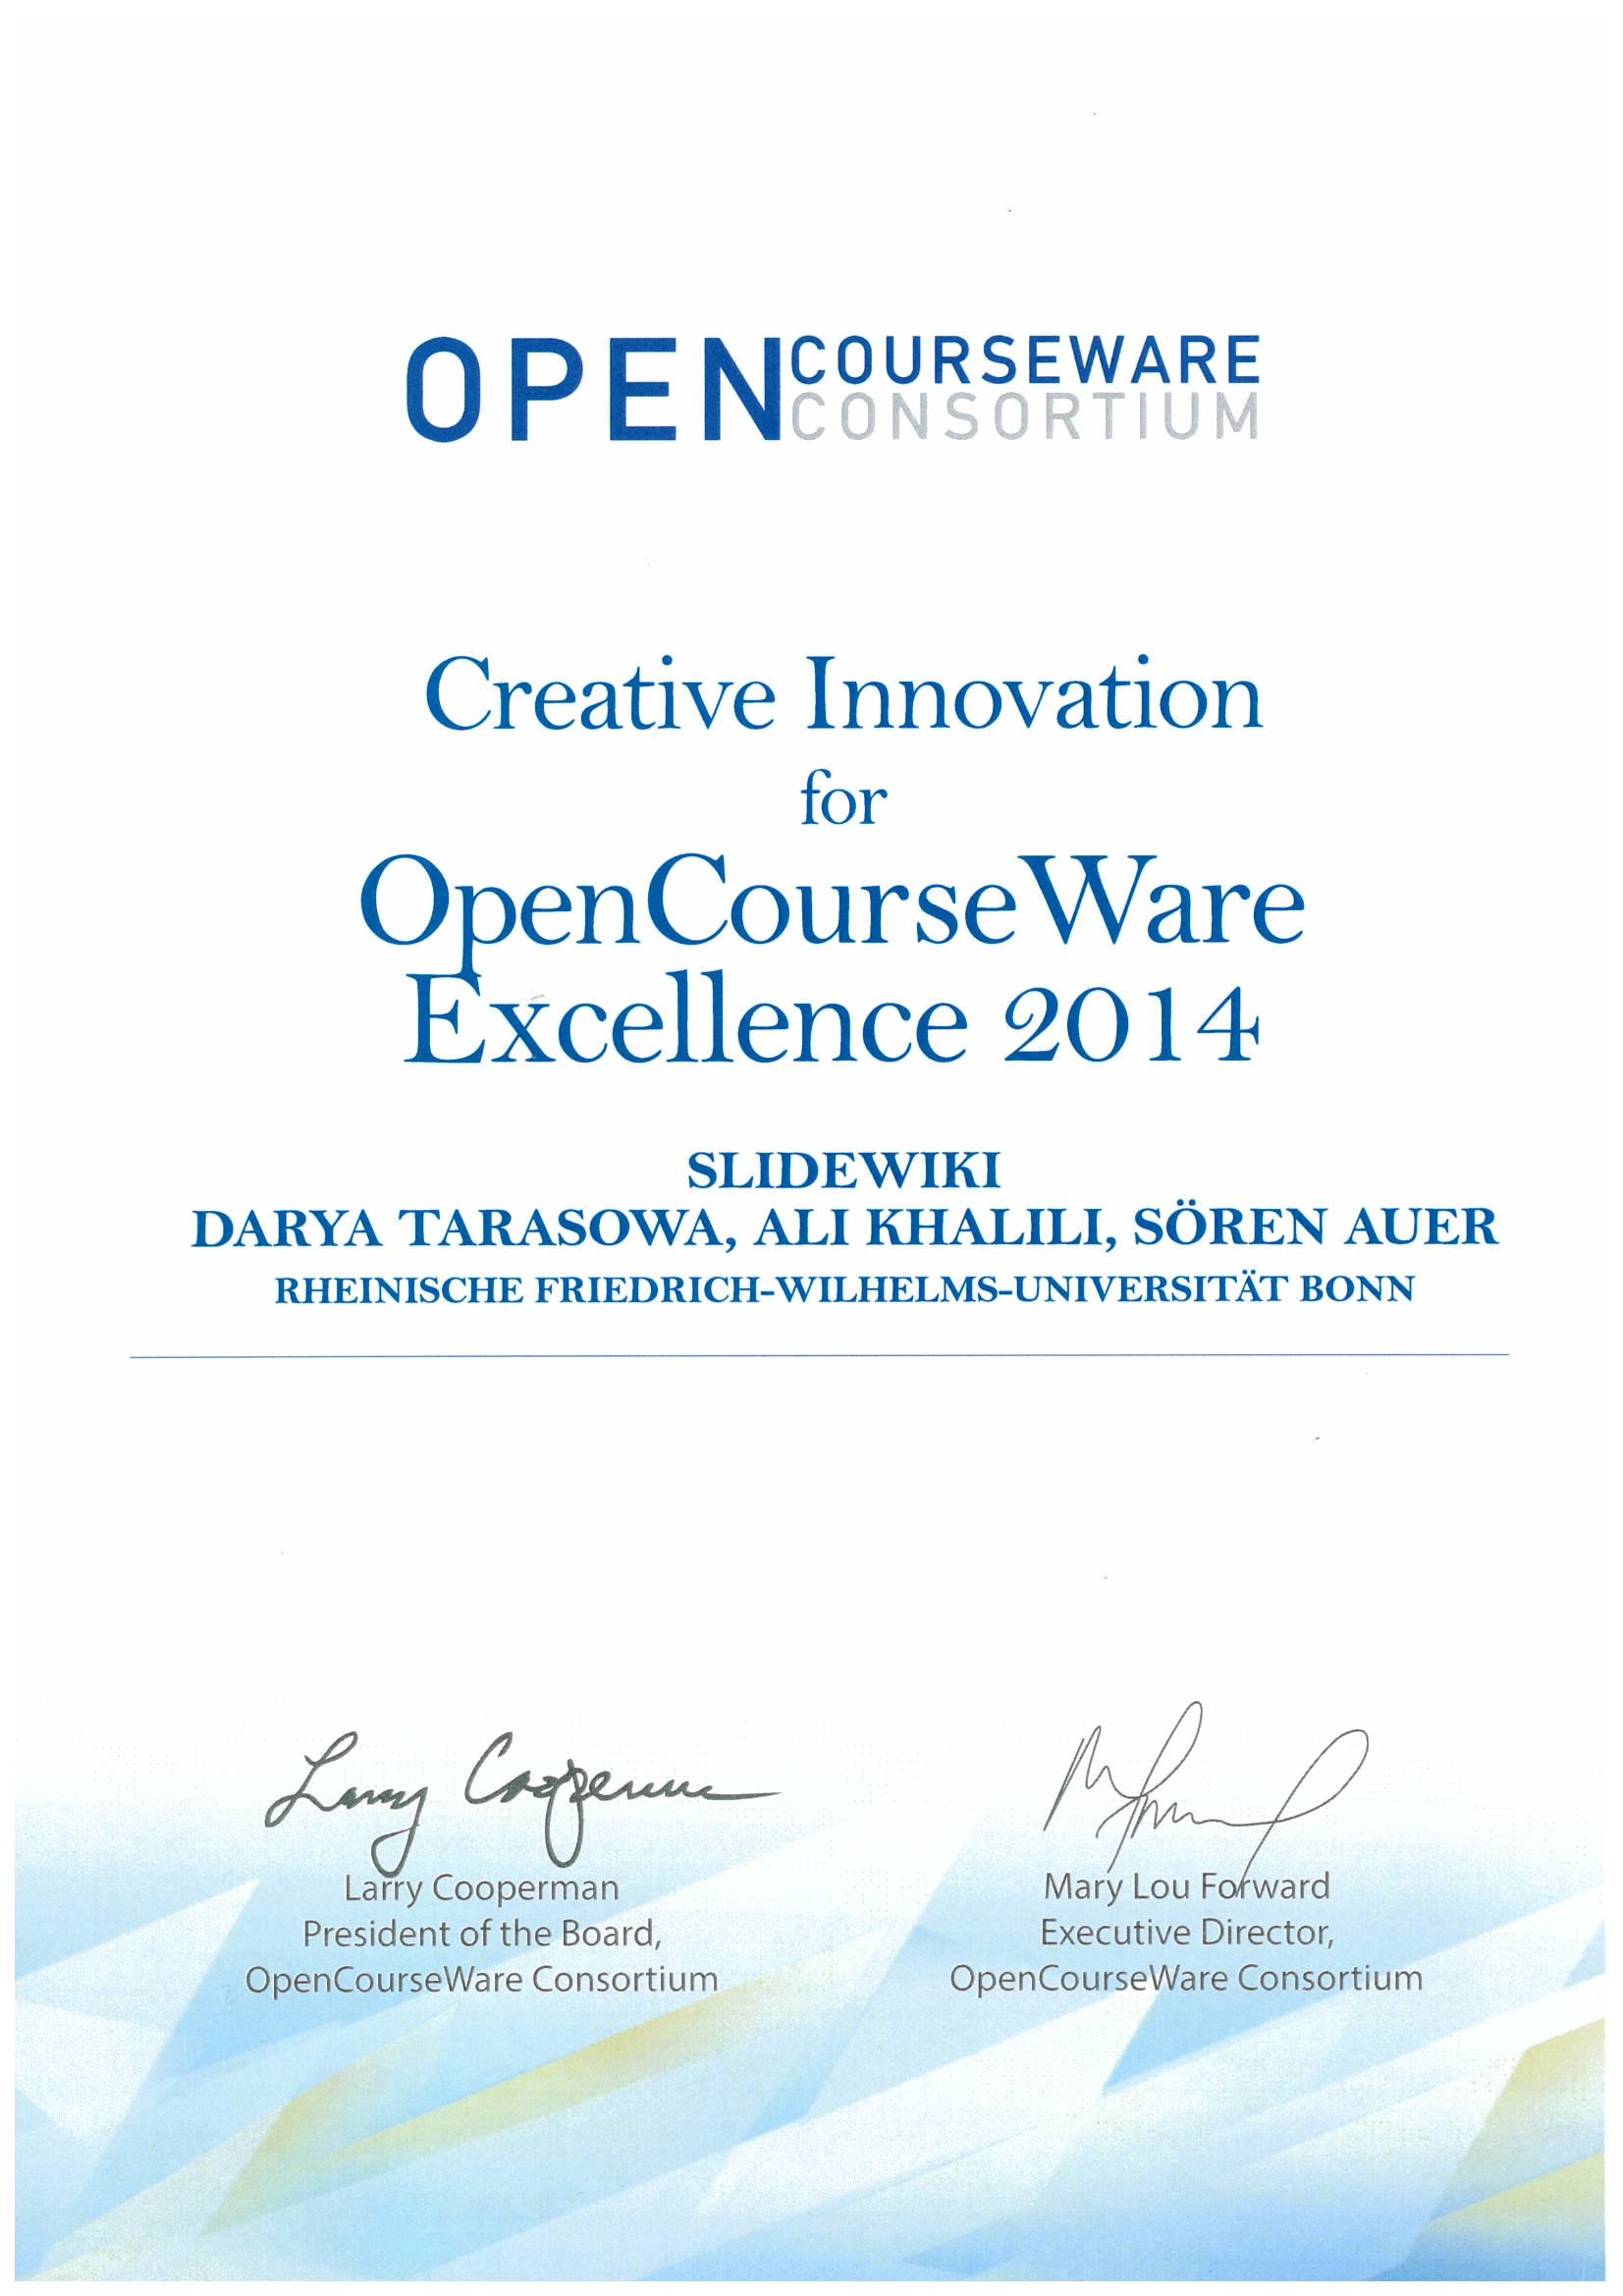
\includegraphics[width=\columnwidth]{images/award.jpg}
\caption{The certificate of the OpenCourseWare Consortium’s Excellence Award for SlideWiki}
\label{fig:ocw_global_award}
\end{figure}

%In this project, the consortium aims to further mature, advance and validate the SlideWiki platform and to integrate it with complementary tools, services and solutions such as Massive Open Online Course (MOOC) platforms and Learning Content Management Systems (LCMS).
%In particular we will pursue the following objectives:
%\paragraph{Objective 1.} Implementation of real-world, large-scale pilots that leverage the power of large-scale collaboration for the creation of inclusive and engaging open content for learning and teaching.
%The pilots should cover a challenging geographic and thematic space and result in a critical mass of engaging open multilingual courseware content, educators and learners as well as supporting organization to establish SlideWiki as the world-leading OCW authoring platform.
%\paragraph{Objective 2.} Reducing the restrictions of time and physical space on learning and teaching through an online platform encouraging asynchronous multi-lingual collaborative content creation and learning, social networking around learning content as well as multi-platform course delivery including ubiquitous accessibility on mobile and smart devices and facilitating the creation of MOOCs. 
%\paragraph{Objective 3.} Foster greater connection between formal, non-formal and informal learning and remove obstacles for ubiquitous learning through social learning analytics and learning mashups. 
%\paragraph{Objective 4.} Link a large space of relevant stakeholders in educational technology with regard to geographic, technologic and learning stage related aspects aiming at support for end-to-end scenarios, where all relevant stakeholders from material provisioning, content production, translation, learning delivery and analytics are integrated into sustainable educational content value chains.
%\paragraph{Objective 5.} Ensuring accessibility and inclusive learning to support children and adults with physical, sensory and cognitive disabilities and impairments who undergo general education, lifelong learning or vocational training through inclusive standard compliant HTML5-based user interfaces for learning and authoring.
%\paragraph{Objective 6.} Skills recognition and validation through learning analytics based on fine-grained content structuring and comprehensive learning self-assessment for each content item.
%As a result, we aim to create a platform facilitating large-scale collaboration around learning content that is similar to Wikipedia with collaboration around encyclopedic content.
%We expect SlideWiki to quickly gain active users, which we deem to reach millions in the end of the project.

The expected project impacts on European education after successful objectives completion include (but not limited to):


%\subsection{Project Overview}
% 
%The project's main aim is to dramatically change the way how courseware is created, shared, translated and used collaboratively without technology getting in the way.
%We envision that SlideWiki can have a similar impact on the educational domain as Wikipedia had on encyclopedias or more recently OpenStreetMaps on online maps.
%Many examples show, that high quality and multilingual content is a key asset on the Web and will attract large user communities.
%With SlideWiki we aim to assemble a vast repository of OpenCourseWare covering as many different domains, languages and learner levels as possible.


%\subsection{Project Objectives}

%
%We expect the project to further influence the European economy and society by bringing dramatic changes in educational material authoring.
%
%\paragraph{Enhance the development of digital learning and teaching resources, including for children and adults with mental or physical disabilities.} 
%Isolated learning resources that are created for specific applications are still an open problem for technology enhanced learning.
%Unlike the content created and maintained by a single author, be it an individual or an organization, the knowledge which is shaped, reviewed, refined and shared by joint contributions and interactions of a group of collaborators with similar backgrounds or interests, holds vast potential to constantly grow, and be enriched and improved. Yet, this potential is often hindered by the lack of tools that would allow the authors working in a collaborative setting to maintain the existing knowledge, synchronize their efforts, communicate and exchange ideas, engage learners, and raise the social awareness in order to bring in even more people that would like to contribute.
%SlideWiki will change the way educational content is put together by introducing new ways to plan, set and reach common goals, communicate, coordinate and build consensus.
%Whether it's educators looking for better ways to represent and transfer their knowledge, or students working in teams / study groups in order to learn something new, or a collaboration between both teachers and learners, SlideWiki will provide its users with the means to share and reunite dispersed pieces of information by connecting them with others whose knowledge complements their own.
%Slidewiki invites not only students, educators, and other professionals (e.g. continuing health/medical education) but also children and adults with mental or physical disabilities to evaluate its outcomes.
%Different levels of education are affected, namely, professional and vocational level, higher education, secondary education  as well as school level.
%This is of paramount importance as it allows an individual to follow SlideWiki and its advancements throughout his/her entire professional life, that is from school to work and staff development life periods.
%Moreover, in order to derive best practices for the development of digital learning and teaching resources, re-use and sharing, the SlideWiki needs a critical mass of educational content as well as content types provided by the involved project and associated partners.
%To this extent, that fact that all levels of education are targeted in SlideWiki is crucial for the establishment of the aforementioned critical mass and outreach.
%In addition, SlideWiki is going to expand the already achieved best practices from past successful projects in the SlideWiki consortium (cf. www.meducator.net, in which critical masses of content types have been aggregated while sharing mechanisms were standardized).
%This finally provides a useful and important continuation at the EU funding level.
%
%\paragraph{Open technologies that grant access to education for everyone.}
%Slide Wiki as well as technology provided by partners has been created in the spirit of open source development. We believe that the process of creating open educational resources and open source software do have much in common. With both you can just use the resources, you don't have to remix or contribute, and there is nothing wrong with that. If you do want to contribute though or you might feel an existing resource is near to what you want, you are free to build on it to meet new challenges.Platforms like OpenCast, which aim at technical tools for creating video based learning material (like large scale lecture capture) received huge uptake in the related international open source domain. Developers from around the world communicating in virtual meetings, change, modify products, designs and content collaboratively to adjust and update the community driven project (e.g.  projects activity stream). Similar is true for the partnering Roberta (learning robot) networks (Open roberta projects activity stream). Consortium members are already active in this development circles which makes it easy to position SlideWiki extensions as affiliated projects in partner development channels to gain the required technical development interest and momentum.
%
%\paragraph{Increase the number of public-private partnerships addressing technological challenges for modernizing and improving technology.}
%The above mentioned affiliated open source projects (see also Letters of Support) already partnering with SMEs (e.g. Teltek, Entwine) and public-private partnerships (e.g. Lower Saxony Elan e.V.)  to safeguard the required service stability from one version to a new version and to adjust the software to certain customer needs which are not directly part of the community product roadmap. SlideWiki brings very welcome technology to this partners and networks by allowing to create slide based presentation content in an standard (e.g. semantics, linked data) and open way. Due to the international collaboration of the involved partner projects we anticipate positive effects along the outreach.
%  
%
%\paragraph{Contribute to the objectives of the European "Opening up Education" initiative.}
%The "Opening up Education" initiative~\footnote{\url{http://www.openeducationeuropa.eu/en/initiative}} is ... \todo{describe the initiative}
%\begin{itemize}
%\item open technologies that grant access to education for everyone
%\item everyone to engage in learning/study groups, thus creating learning communities beyond their classrooms 
%\item make personalisation and customisation of education a much easier task
%\item teachers to create communities of practice to exchange teaching materials and best practices; 
%\item provide access to a wider range of educational resources across borders and languages.
%\end{itemize}
%
%\paragraph{Increase the number of public-private partnerships addressing technological challenges for modernizing and improving education and training.}
%
%\begin{itemize}
%\item we can invite enterprises for smaller trials, discussing and adapting the content and formats to their needs
%\item as the content can be easily converted to many formats, content produced by academics can be easily adapted and integrated in enterprise learning systems and vice versa. 
%\item SlideWiki can play a role of communication platform between the two stakeholders, where they can discuss issues and the ways to solve them
%\end{itemize} 




\paragraph{Impact on secondary Education and Higher-Education.}
The intended system components and services will invite learners, educators, and other professionals to evaluate its outcomes and use the community created content in their own context.
All three levels of tertiary education are affected, namely, undergraduate, postgraduate, and further.
This is of paramount importance as it allows an individual to follow SlideWiki and its advancements throughout his/her entire professional life, that is from college to work and staff development life periods.
Moreover, in order to derive the best practices for educational content reuse and sharing, the SlideWiki needs a critical mass of educational content as well as content types.
To this extent, that fact that all levels of education are targeted in SlideWiki is crucial for the establishment of the aforementioned critical mass.
			
\paragraph{Impact on professional and vocational training.}
Existing online learning resources often used by life-long learners lack engagement mechanisms.
For instance, Massive Open Online Courses show really big dropout rates (90\% following some studies).
This constitutes one of the main risks for online educational initiatives given the amount of resources (platform, bandwidth, teaching assistants time, learners time etc.) that are wasted.
Consequently, one of the main contributions of a successful online educational initiative like SlideWiki is to reduce dropout rates by engaging learners.
This will be done by better adapting content and the learning experience to user needs, something possible and easier as content is really open and contributions encouraged.
Moreover, the social components included will also engage users through group learning, gamification and social interactions.

\paragraph{Impact on Open Education Community.}
We expect SlideWiki and its surrounding services to become a catalyst in the establishment of an European Open Education community.
The value produced by the large amount of high-quality multilingual courseware being freely available through the service, the large user community and the positive overall image this no-for-profit service accumulates, will attract a large number of stakeholders to join this initiative and its aim of establishing a European Open Education community.
We expect universities, companies, institutions of higher education, school authorities, grass-roots initiatives, companies in the education field and many others to join the activities and events started and spun-off from this project.

\paragraph{Further expected economic impacts}
Wikipedia and other projects have been perfecting and evolving the community-source approach to pooling resources, knowledge sharing, leveraging and aggregating wisdom with user support to create attractive solutions that used by thousands of different users with manifold experience and backgrounds everyday.
We envision to pool individual, community, and university resource contribution and intellectual capital investments and leverage them to create sharable and accessible Open Educational solutions that are of, by, and for schools, teachers, higher education as well as companies and learners around the world.
As a community driven project, SlideWiki will employ the development principles of open source software.
We are aiming at solving challenges together with our collaborating networks to make SlideWiki a reliable service companion for existing enterprises as well as for beginners that want to build upon this investment adapting the content and formats to their needs. 

\paragraph{Further expected societal impacts}
Universities want to go where the learners are to share their rich scientific and intellectual knowledge beyond the walls of the academy and to expand the boundaries of the classroom.
Many people have just experienced education as courses they learn from. 
Often OERs are just thought of as free courses, but the opportunity to involve users within the creation process (without losing track of changes and authorship) gives us a chance to make learning more engaging and active.
OERs need to be useful in many different channels (mobile, social web, blog, wikis, internal company networks, etc.) to rise the societal impact by providing direct benefit to the context they are being used.
Further aspects include the demand to insert cultural specific references to make a concept easier to understand for a different group (school kids, foreign culture, etc.).
SlideWiki as a platform depends on partnering organizations and their established network outreach.
Through the projects participating organizations and involved parties we expect an easy and welcome uptake of the described idea and technology which increases the societal impact.



\appendix

%------------------------------------------------------------------------------
\chapter{Research Paper: Measuring the quality of relational to RDF mappings}
\label{sec:app_rdb2rdf}
%------------------------------------------------------------------------------

\section{Abstract}
Mapping between relational data and linked data (RDB2RDF) is an essential prerequisite for evolving the World Wide Web into the Web of Data.
We propose a methodology to evaluate the quality of such mappings against a set of objective metrics.
Our methodology, whose key principles have been approved by a survey among RDB2RDF experts, can be applied to evaluate both automatically and manually performed mappings regardless of their representation.
The main contributions of the paper are: (1) assessing the quality requirements for mappings between relational databases and RDF, and (2) proposing methods for measuring how well a given mapping meets the requirements.
We showcase the usage of the individual metrics with illustrative examples from a real-life application.
Additionally, we provide guidelines to improve a given mapping with regard to the specific metrics. 

\section{Introduction}

Translating the data stored in relational databases (RDB) to the linked data format is an essential prerequisite for evolving the current Web of documents into a Web of Data.
In order to be effectively and efficiently reusable, linked data should meet certain data quality requirements~\cite{Zaveri}.
Assessing the quality of a linked dataset created from RDB may be a laborious, repetitive task if the dataset is frequently recreated from its RDB source, e.g.\ after any update to the RDB.
We therefore claim that it is possible to positively influence the quality of a linked dataset created from RDB by improving the quality of the RDB2RDF \emph{mapping} that produces the linked data\footnote{Here, we use the term ``mapping'' to refer to the function that maps relational database columns to RDF properties, but not to materialisations of such mappings in concrete languages or representations, nor to tools that would execute such a function.}.
To the best of our knowledge there has not been prior research towards collecting and describing quality requirements for RDB2RDF mappings.
Thus, this paper aims to fill the gap by providing a system of metrics to measure the quality of RDB2RDF mappings.

A large number of tools for mapping relational data to RDF exist already\footnote{One of the listings is available at \url{https://github.com/timrdf/csv2rdf4lod-automation/wiki/Alternative-Tabular-to-RDF-converters}.}; they implement different mapping approaches, often allowing to customize the mapping.
To standardize the description of mappings, the W3C RDB2RDF Working Group has released two recommendations in 2012 (more details in~ Section\ref{sec:mapping-quality}): Direct Mapping~\cite{direct_mapping}, which produces RDF graph representations directly from a relational database (data and schema) and the Relational Database to RDF Mapping Language (R2RML)~\cite{r2rml} for expressing customized mappings.
 
In this paper, we aim at developing a system of quality metrics that can be applied both to direct and customized mappings that works with different representations of mappings (R2RML or proprietary formats, visual diagrams, tables, etc.).
Any of these representations are suitable for being evaluated with the proposed system as long as one can derive a list of database columns (including unmapped ones) and their corresponding RDF properties (for mapped ones).

To determine the scope of requirements that can be posed to RDB2RDF mappings, we studied the state of the art in related research fields such as ontology matching, linked data quality assessment and RDB2XML mappings. 
However, as Section~\ref{related_work} shows, these metrics collected from the scientific community do not solve the given problem entirely.
In order to fulfil the list, we followed the Direct and R2RML Mapping recommendations.
Some of the RDB2RDF features standardized in the documents are connected with the output data quality dimension, while others influence the quality of the mapping itself. 
For example, the ability to define R2RML views allows to incorporate domain semantics into the mapping – an opportunity that we consider to increase the quality of mapping.
We propose not only a system of metrics but also define means of measuring them, along with guidelines to improve the rating of a dataset w.r.t.\ each metric.

The paper is structured as follows: in Section~\ref{related_work} we discuss the existing approaches, in Section~\ref{requirements} we summarize the quality requirements for mappings and the metrics for measuring the quality.
\hyperref[evaluation]{Section~\ref*{evaluation}} presents the results of the survey conducted in order to collect the community feedback.
In Section~\ref{conclusions}, we conclude and propose future research directions.

\section{Related work}
\label{related_work}

\paragraph{RDB2RDF mapping approaches.}
Although previous research has not explicitly focused on collecting requirements for RDB2RDF mappings, many such requirements can be found in best practice and mapping approach descriptions.
For instance, in \cite{hillairet2008mde}, the importance of reusing existing vocabularies to enhance the interoperability of the output dataset is explained.
We extend this statement to a set of requirements combined in the \emph{interoperability} dimension, taking into account not only quantitative, but also qualitative metrics.

We notice that existing literature on the topic uses incoherent terminology.
Often, the term \emph{mapping} is used instead of mapping \emph{language}, e.g.\ in~\cite{Auer2010,Erling2008}. 
Discussing the requirements for mapping \emph{language}, both articles mention the following requirements for RDB2RDF \emph{mapping} as well:

\begin{itemize}
\item presence of both ETL and on-demand implementation
\item incorporating domain semantics that is often implicit or not captured at all in the RDB schema
\item indication of time metadata about the dataset during the mapping creation process to control the dataset currency (we subsume this metric under “data quality”)
\item intensive reuse of the existing ontologies
\end{itemize}    

\paragraph{Requirements for mappings between relational data and XML.}
The topic of mapping relational data to \emph{XML} is related to RDB2RDF mapping due to the similarity between the XML and RDF data models.
The earliest articles on the quality of RDB2XML mappings (e.g.~\cite{Schmidt, Shanmugasundaram}) only take into account the performance of the mapping algorithms.
This is because RDB2XML mappings are mostly produced automatically and do not allow customization.
Only few authors (e.g.~\cite{sahuguet2001everything}) propose metrics for evaluating the quality of the output data.
However, the proposed metrics evaluate only the syntactic correctness of the output XML and therefore cannot be applied to documents in RDF (except for \emph{presence of syntax errors}).

Other approaches (e.g.\ \cite{he1999relational}) prove the need for customizable techniques of mapping due to the wide gap between these two formats.
As their major evaluation criterion, they use the \textit{efficiency of query processing}.
We adopt this approach and base our \textit{simplicity} metric on it.
Liu et al.~\cite{liu2006designing} describe an approach to design a high-quality XML Schema from ER diagrams.
The authors define a list of requirements for the design; the most relevant one for our purposes is \emph{information preservation}.
However, the metrics for \emph{measuring} such requirements are not discussed.
We study the information preservation requirement in detail and provide objective metrics in the \emph{Faithfulness of Output} dimension.

\paragraph{Requirements for ontology matching.}
Mapping between a database schema and an RDF vocabulary can also be viewed as a special case of ontology matching.
Several studies propose requirements for measuring the quality of an ontology matching.
According to~\cite{euzenat2007ontology}, all proposed measures can be distinguished between compliance measures, measures concerned with system usability and performance measures focusing on runtime or memory usage.
As our study focuses on evaluating the quality of mapping itself, we do not take the system usability or performance dimensions into account.

In the evaluation of ontology matching, compliance measures are based on the two classical information retrieval measures of \emph{precision} and \emph{recall}~\cite{vanRijsbergen}.
We adapt these metrics to the evaluation of RDB2RDF mappings and include them in the \emph{faithfulness of output} dimension as \emph{coverage} and \emph{accuracy of data presentation} metrics. 

\paragraph{Measuring linked data quality.}
The quality of mapping correlates with the quality of output linked data produced by the mapping.
Poor design decisions made at the stage of defining a mapping, such as using deprecated classes, redundant attributes or badly formed URIs, decreases the quality of the output data.
Therefore, metrics for the quality of the output data can be viewed as metrics for quality of the mapping.

The field of assessing the quality of linked data is still in its infancy, but several articles have addressed it already. 
Our recent survey~\cite{Zaveri} collects and compares the existing papers, 
the most complete and detailed ones being Bizer's PhD thesis~\cite{bizer2007quality}, Flemming's master's thesis~\cite{flemming} and empirical evaluations by Hogan et al.\ \cite{hogan2010weaving, hogan2012empirical}. 
The survey provides formal definitions of data quality dimensions and metrics as well as evaluates existing tools for (semi-)automatic measurement of linked data quality.

The current paper assumes that the quality of a linked dataset is influenced by the mapping that produces it and thus categorizes the metrics from the survey from the perspective of the RDB2RDF mapping.
We select those metrics that are related to the mapping process and adapt them to the RDB2RDF domain.


\section{Quality Requirements}
\label{requirements}

This section gives a detailed overview of the proposed quality requirements for RDB2RDF mappings, ways of measuring them (metrics) and guidelines for improving mappings w.r.t.\ these metrics.
Our proposed system incorporates four quality dimensions with 14 objective metrics overall.
For assessing the overall quality of a mapping, one would, in practice, assign \emph{weights} to the metrics.
Their choice depends on the goal of the mapping process.
For example, when the goal of the mapping is to accurately represent the relational data,
the metrics in the “faithfulness of the output” dimension should be assigned the highest weight.

\begin{table*}[!ht]

	\centering		
	\begin{tabulary}{\textwidth}{LLL}
	\toprule
		\textbf{{Requirement}} & \textbf{{Description}} & \textbf{{Measure}} \\
		\midrule
		
		\multicolumn{3}{c}{\textbf{Quality of the mapping implementation and representation}} \\
\hline
		\textbf{Data accessibility} &
Describes how the mapping result can be accessed. 
		 & ETL/on-demand/both\\
\hline
		\textbf{Standard compliance} &
Characterizes if the mapping representation is standard compliant.
		 & boolean \\
\hline
		 
		\multicolumn{3}{c}{\textbf{Faithfulness of the output}} \\		
\hline
		\textbf{Coverage} & Characterizes the mapping completeness  & percentage of DB columns mapped  \\
\hline
		\textbf{Accuracy of data representation} & Characterizes the mapping correctness & percentage of correctly mapped DB columns \\
\hline
		\textbf{Incorporation of domain semantics} & Shows level of domain semantics incorporation & percentage of properties that link to the results of SQL queries \\
\hline
		
		\multicolumn{3}{c}{\textbf{Quality of the output}} \\		
\hline
		\textbf{Simplicity} & Shows the simplicity of SPARQL queries returning the frequently demanded values & percentage of complex SQL queries results integrated into the mapping \\
\hline
		\textbf{Data quality} & Characterizes the quality of output data & aggregation of linked data quality metrics ($\to$ \autoref{tab:data_quality_groups})\\
\hline
		\textbf{Data integration} & Characterizes the interlinking degree of the output data & percentage of external instances integrated into the resultant dataset\\	
\hline
		
		\multicolumn{3}{c}{\textbf{Interoperability}} \\		
\hline
		\textbf{Reuse of existing ontologies} & Shows the amount of reused vocabulary elements & percentage of reused properties and classes\\
\hline
		\textbf{Quality of reused vocabulary elements} & Characterizes the quality of chosen for reuse properties and classes & accumulated quality and popularity of reused vocabulary elements \\
\hline
		\textbf{Accuracy of reused properties} & Characterizes the accuracy of properties reuse & percentage of accurately reused properties \\
\hline
		\textbf{Accuracy of reused classes} & Characterizes the accuracy of classes reuse & percentage of accurately reused classes  \\
\hline
		\textbf{Quality of declared classes/properties} & Shows the quality of ontology documentation & accumulated quality of declared classes/properties\\
\hline
	
	\end{tabulary}
		
	\caption{Summary table of proposed metrics system}
	\label{tab:summarytable}
\end{table*}

\subsection{Quality of the mapping implementation and representation}
\label{sec:mapping-quality}
The requirement of mapping quality implementation and representation combines the requirements for resultant data accessibility and standard compliance of the mapping representation.

\paragraph{Data accessibility.}
Data accessibility describes how the result of the mapping is accessed. 
This metric is also known in the literature as “access paradigm”, “mapping implementation” or “data exposition”~\cite{spanos2012bringing}.
There are two possibilities: (i) Extract Transform Load (ETL) and (ii) on-demand mapping.
According to~\cite{Erling2008}, ETL means physically storing triples produced from relational data in an RDF store.
The disadvantage of ETL is that that, whenever the RDB is updated, you have to re-run the entire ETL process, even if just one RDB record has changed, carrying out an often redundant synchronization process.
However, in the ETL case nothing more than the RDF store is needed to answer a query.

On-demand mapping is realized by translating a SPARQL query into one or more SQL queries at query-time, evaluating these against (a set of) unmodified relational database(s) and constructing a SPARQL result set from the result sets of such SQL queries.
In contrast to the ETL implementation, on-demand mapping requires more resources for processing each query.
However, the on-demand implementation does not face the synchronization issue and does not replicate the data.  
In the light of these advantages and disadvantages, we claim that the best solution is to implement a mapping with both data access approaches.
Thus, the index of implementation takes a value equal to 1, if both implementations are present and 0.5 otherwise.


\paragraph{Standard compliance.}

An RDB2RDF mapping can either be represented as a set of customized rules or through a generic set of rules (as defined by the W3C Direct Mapping standard~\cite{direct_mapping, Bertails_2011}).
Often, the output of a Direct Mapping may not be useful, that is, it may not adequately take the structural/semantic complexity of the database schema into account.
Thus, while the applicability of a Direct Mapping satisfies the requirements for the “standard representation” metric, not using the customized rules will lead to a loss of points w.r.t.\ other metrics.

Languages for representing customized mappings have been surveyed in~\cite{spanos2012bringing}.
Until recently, no standard representation language for RDB2RDF mappings existed, however, as of 2012, R2RML~\cite{r2rml} has been released as a W3C recommendation.
As it is the only mapping language that has been standardized to date, we do not consider other (proprietary) formats reasonable.

Thus, we propose that if there is no material representation of a mapping available, it should be assumed that a Direct Mapping is carried out.
We define the “standard representation” metric to be one if the mapping is represented in \emph{R2RML} or if there is no representation (and therefore a Direct Mapping is applicable), and zero otherwise.
 
\subsection{Faithfulness of the output}
In terms of RDB2RDF mapping we define the faithfulness of output as an abstract measure of similarity between the source data and resultant dataset.

\paragraph{Coverage.}
This metric indicates the ratio of the database columns mapped to the RDF. 
In general, a high coverage increases the faithfulness of the output data.
However, reaching the highest level of coverage may conflict with privacy restrictions.
Therefore, great care should be taken when mapping any kind of personal (sensitive) data that might be linked with other data sources or ontologies.
It may even be illegal to create or to process such linked information in countries with data protection laws without having a valid legal reason for such processing~\cite{bechhofer2004owl}.
 
Moreover, application-specific data such as statistics of usage or service tables often are not included into the mapping due to its application-related nature.
Thus, in real-world applications, the coverage metric never reaches one.
%scale

\paragraph{Accuracy of data representation.}
When mapping relational data to RDF, the accuracy of data representation is tightly connected to data formatting issues.
For example, differences in the representation of numeric values between the database and RDF can cause inaccuracies in the output data.
Inaccurate dealing with not-Latin characters leads to loss of data meaning. 
We propose the following algorithm to evaluate the accuracy index of the mapping:

\begin{enumerate}
\item\label{it:avg-database} for each mapped database column containing numeric data, compute the average value of the numbers in this column;
\item find an average value for the corresponding property in the RDF output, and compare it to the average computed in step~\ref{it:avg-database};
\item\label{it:num_points} add a point for each coinciding average (considering the statistical error)
\item\label{it:lit_points} for each mapped database column containing literal data, analyze the readability of the corresponding properties; add a point for each completely readable property;
\item calculate a sum of the points obtained in steps~\ref{it:num_points} and~\ref{it:lit_points} and divide the sum on the total number of columns mapped.
\end{enumerate}

\paragraph{Incorporating domain semantics.}
\label{par:dom_semantic}

The incorporation of domain semantics is one of the crucial aspects that indicate the quality difference between direct and customized mappings. 
Measuring this requirement helps to estimate the direct benefit of mapping customization.
Generally, a direct mapping does not incorporate domain semantics; in this case the metric takes a value of zero. 
The extent of domain semantics incorporation can be measured by counting number of \emph{class properties} which take values from any database table \emph{other than} the table that corresponds to a class.
The metric is then calculated as the ratio between this number and the  count of properties summed up over all classes in the mapping.

To improve the mapping w.r.t.\ this metric, implicit relations between the data in the database should be explicitly modelled in the mapping.
This process also increases the simplicity of the mapping, as it requires integration of the SQL query results into the mapping, thereby simplifying (future) SPARQL queries for obtaining these values. 

\subsection{Quality of the output}

Quality of the output combines requirements of the output data quality in aspects of simplicity of usage, level of interlinking and objective data quality metrics.

\paragraph{Simplicity.}
One often has the task of mapping highly complex data models to RDF.
In that case, Direct Mapping produces an RDF output that may be difficult to use, especially when considering the limitations of the SPARQL query language.
Thus, useful information from the source database may lose its value in the RDF dataset that results from mapping.
Metrics for the quality of the output should therefore take the simplicity of the RDF dataset into account.
By simplicity of RDF data, we mean the simplicity of \emph{operating} on it.
In other words, the simplicity of data determines the simplicity (or length in terms of abstract syntax) of the SPARQL queries returning frequently demanded values.  
To increase the simplicity, the mapping should aim to produce a dataset, that can be queried for frequently demanded values by relatively simple SPARQL constructions. 
To do this, the \emph{frequently demanded values returning by the complex SQL queries} should be integrated into the mapping.
Such preparations not only increase the simplicity of the output, but also \emph{incorporate domain semantics} not presented in the relational database explicitly (cf. Section~\ref{par:dom_semantic}).

To calculate the index of simplicity, first a list of complex SQL queries should be assembled.
We propose to consider a query “complex” in the following cases:
\begin{itemize}
\item a query joins at least two tables or views,
\item a query supposes recursive computations over one table or view.
\end{itemize}
After the list is assembled, frequently demanded values, returned by the queries should be selected.
This selection is subjective and should be carried out by a group of developers and administrators of the project.
The simplicity metric is then calculated as the percentage of \emph{frequently demanded values returned by complicated SQL queries} that have been integrated into the mapping. 

\paragraph{Data quality.}
\label{data_quality_par}
The quality of a mapping can partly be assessed by evaluating the quality of the output RDF data.
Section~\ref{related_work} points to approaches for assessing data quality.
However, when evaluating the quality of a mapping, not all aspects of output data quality need to be taken into account.
This is due to the fact that not all aspects of linked data quality are affected by the mapping stage.

\begin{table}[!tb]
\scriptsize
\centering
\begin{tabular}{p{0.52\linewidth}|p{0.46\linewidth}}
\toprule
\multicolumn{2}{c}{\textbf{Requirements for linked data quality and their metrics}} \\

\midrule
\myparagraph{1. Influenced by mapping}
\begin{itemize}
\item \textbf{Completeness:} influenced by coverage
\item \textbf{Validity-of-documents:} influenced by quality and accuracy of reused and newly determined classes
\item \textbf{Interlinking:} influenced by data integration 
\item \textbf{Availability:} influenced by dereferenceability of reused and newly defined classes
\item \textbf{Consistency:} influenced by reuse
\end{itemize}



\myparagraph{2. Depend on mapping} 
\begin{itemize}
\item \textbf{Provenance:} indication of metadata about a dataset
\item \textbf{Verifiability:} verifying publisher information, authenticity of the dataset, usage of digital signatures
\item \textbf{Licensing:} machine-readable/human-readable license, permissions to use the dataset, attribution, Copyleft or ShareAlike
\item \textbf{Validity-of-documents:} no syntax errors
\item \textbf{Consistency:} entities as members of disjoint classes, usage of homogeneous datatypes, misplaced classes or properties, misuse of \texttt{owl:datatypeProperty} or  \texttt{owl:objectProperty}, bogus \texttt{owl:Inverse-FunctionalProperty} values, ontology hijacking
\item \textbf{Conciseness:} redundant properties/instances, not-unique values for functional properties, not-unique annotations
\item \textbf{Performance:} no usage of slash-URIs, no use of prolix RDF features
\item \textbf{Understandability:} human-readable labelling of classes, properties and entities by providing \texttt{rdfs:label}, human readable metadata
\item \textbf{Interpretability:} misinterpretation of missing values, atypical use of collections, containers and reification
\textbf{Currency:} currency of data source
\item \textbf{Volatility:} no timestamp associated with the source
\end{itemize}


&

\myparagraph{3. Depend on relational data}
\begin{itemize}
\item \textbf{Completeness:} values for a property are not missing
\item \textbf{Amount-of-data:} see \cite{Zaveri}
\item \textbf{Provenance:} trustworthiness of RDF statements, trust of an entity, trust between two entities, trust from users, assigning trust values to data/-sources/rules, trust value for data
\item \textbf{Believability:} see \cite{Zaveri}
\item \textbf{Accuracy:} see \cite{Zaveri}
\item \textbf{Consistency:} no stating of inconsistent property values for entities, literals incompatible with datatype range
\item \textbf{Interpretability:} interpretability of data
\item \textbf{Versatility:} provision of the data in various languages
\end{itemize}

\myparagraph{4. Depend on publishing} 
\begin{itemize}
\item \textbf{Availability:} accessibility of the server, accessibility of the SPARQL end-point, accessibility of the RDF dumps, no structured data available, no dereferenced back-links
\item \textbf{Performance:} see \cite{Zaveri}
\item \textbf{Security:} see \cite{Zaveri}
\item \textbf{Response-time:} see \cite{Zaveri}
\item \textbf{Conciseness:} keeping URIs short
\item \textbf{Understandibility:} indication of one or more exemplary URIs, indication of a regular expression that matches the URIs of a dataset, indication of an exemplary SPARQL query, indication of the vocabularies used in the dataset, provision of message boards and mailing lists
\item \textbf{Versatility:} provision of the data in different serialization formats, application of content negotiation
\item \textbf{Currency:} see \cite{Zaveri}
\item \textbf{Timeliness:} see \cite{Zaveri}
\end{itemize}


\\
\bottomrule
\end{tabular}
\caption{Data quality metrics divided into four groups according to the stage of mapping creation, on which they can be influenced.}
\label{tab:data_quality_groups}
\end{table}

We confine ourselves to the objective requirements discussed in~\cite{Zaveri} and divide them into four groups (cf.~\autoref{tab:data_quality_groups}):

\begin{itemize}
	\item Requirements that are influenced by mapping quality implicitly.
		Increasing the quality of the mapping in turn increases the quality of data.
	\item Requirements that are influenced by mapping explicitly.
		The proposed data quality index discussed below aggregates these metrics.
	\item Requirements that depend on the quality of data stored in the database. 
		We consider these metrics to be out of the scope of this paper.
	\item Requirements that depend on the quality of linked data publishing.
		We do consider these metrics to be out of the scope of this paper.
\end{itemize}

The metrics and methods of measuring them are discussed in detail in~\cite{Zaveri}.
To evaluate the quality of mapping with regard to output data quality we propose to aggregate only the metrics explicitly depending on the mapping.
There are two possible strategies for calculating our overall data quality metric based on the individual metrics: assigning the same weight to all individual metrics, or assigning different weights to different dimensions or even to individual metrics.

\paragraph{Data integration.}
The key advantage of Linked Data is its ability to effectively integrate data from disparate, heterogeneous data sources.
In most cases, the output dataset resulting from a mapping can be linked to existing datasets via explicitly modelled relationships between entities.
As mentioned in~\cite{sahoo2009survey}, the use of domain ontologies along with user defined inference rules for reconciling heterogeneity between multiple RDB sources, is an effective integration approach for creating an RDF. 
A simple metric for data integration can be defined as the number of external datasets linked to the one evaluated.
However, this metric cannot be mapped to a value in the interval $[0,1]$ in an obvious way, as needed for computing the overall mapping quality from the values of the individual metrics.
Thus, we propose an alternative measure to evaluate the data integration level: index of data integration.
It can be calculated as the ratio between the number of external instances integrated in the resulting RDF dataset and the total number of instances.

\subsection{Interoperability}
\label{inter}

The interoperability requirement tackles the aspect of a mapping to produce interoperable data, which can be easily linked to and integrated with other ontologies and datasets.

\paragraph{Reuse of existing ontologies.} 
The reuse of existing ontology elements (i.e.\ classes and properties), increases the interoperability of the output dataset.
Additionally, this reuse prevents one from having to introduce new elements. 
This requirement can be measured using two metrics: the ratio of reused properties and the ratio of reused classes.
However, not only the quantity, but also the \emph{quality} of reused properties and classes is important.
This aspect is covered by the next metric.

\paragraph{Quality of reused vocabulary elements.}
\label{par:quality_reused}
Measuring the quality of reused properties or classes is not trivial.
As a large number of vocabularies has been published on the Web, many vocabulary elements are repeatedly declared instead of being reused.
We claim that the best choice of a class or property to reuse depends on two parameters:
(i) the quality of the class or property itself and 
(ii) the frequency of its usage in LOD in comparison with semantically similar alternatives.
Thus, to measure the quality of each individual property or class we propose the following workflow: 
\begin{enumerate}
\item Measure the quality of the chosen vocabulary element (class/property)
\item Find alternatives to the chosen element and measure their quality
\item Compare the quality metrics of the chosen element and the best alternatives
\end{enumerate}

We propose to compute the quality index ($i_\mathit{qual}$) of the chosen vocabulary element as the product of the following two indexes:
the index of documentation quality ($i_\mathit{doc}$) and the index of popularity ($i_\mathit{pop}$).
The proposed index of documentation quality is computed differently for classes and properties.
Both for classes and properties, the index of documentation quality takes into account dereferenceability as well as documentation by \texttt{rdfs:label} and \texttt{rdfs:comment} (preferably in multiple languages).
If the class or property is explicitly deprecated, i.e. its \texttt{owl:deprecated} annotation property equals \texttt{true}, we define its quality index as zero.
Additionally, for classes, their relation to other classes should be indicated (rdfs:subClassOf or owl:equivalentClass).

For properties, \texttt{rdfs:range} and \texttt{rdfs:domain} should be defined.
Based on the presence of the properties definitions mentioned above, a decision about quality of the documentation for a vocabulary element (possibly automated) should be made.
The index of popularity aims to measure the frequency of usage of the class or property on the Web in comparison with semantically similar alternatives.
This index can be taken from services such as Linked Open Vocabularies\footnote{http://lov.okfn.org}.

As an example, we evaluate the property \texttt{agrelon:hasChief}\footnote{full URI: \texttt{http://d-nb.info/standards/elementset/agrelon.owl\#hasChief}} that links an \emph{organization} to its \emph{chief}.
The property is dereferenceable, it has labels available in four languages; however, no \texttt{rdfs:range}, \texttt{rdfs:domain} or \texttt{rdfs:comment} is specified.
Based on this, we define its $i_\mathit{doc}$ as 0.5.
For measuring the frequency of usage we type the term `chief' into the search field of the Linked Open Vocabularies service. 
Looking through the results, we can conclude that on the Web of Data the term `chief' is most commonly used to model a military commander and the chosen property \texttt{agrelon:hasChief} has a low popularity metric value of 0.271.
Thus, the quality index for this evaluated property is $i_\mathit{pop} * i_\mathit{doc} = 0.271 \cdot 0.5 = 0.1355$.

The next task is to find the most commonly used term for the evaluated property.
The list of possible substitutes will include properties matching `chief', `leader', `head', or `boss'.
For each item on the list the property with the highest $i_\mathit{pop}$ and satisfying the following requirements, should be found:
\begin{itemize}
\item \texttt{rdfs:comment}, \texttt{rdfs:domain} and \texttt{rdfs:range} statements should correspond to the domain model
\item depending on the application settings, special requirements such as presence of an inverse property in the same vocabulary may need to be satisfied. 
\end{itemize}

In our case, the metrics for the best candidates are represented in Section~\ref{sem_identical}.
Due to space limitations, we only take into account the first two synonyms from that list, as the two other ones do not have matches that satisfy the requirements given above.
According to the investigation, the \texttt{agrelon:hasChief} property is not the best possible alternative for linking an organization to its chief.
The \texttt{swpo:hasLeader} property should be used instead, as its quality index is $i_\mathit{pop} \cdot i_\mathit{doc} = 0.682 \cdot 0.8 = 0.5456$.

\begin{table}[!htb]
\centering
\begin{tabulary}{\columnwidth}{L|L|L}

\toprule
& \textbf{`chief'} & \textbf{`leader'}  \\
\midrule
best candidate & agrelon:hasChief & swpo:hasLeader  \\
\textbf{$i_\mathit{pop}$} & 0.271 & 0.682  \\
\textbf{$i_\mathit{doc}$} & 0.5 & 0.8 \\
\textbf{$i_\mathit{qual}$} & \textbf{0.1355} & \textbf{0.5456} \\
\end{tabulary}
\caption{Metrics for semantically identical properties to link an organization and its chief}
\label{sem_identical}
\end{table}

The last step is to compare the quality of the chosen property and the best possible alternatives.
The resultant score for the chosen property is calculated as the ratio between its quality index and the quality index of the best possible alternative: $i_{\mathit{qual}_\mathit{chosen}} / i_{\mathit{qual}_\mathit{best}}$ where $i_{\mathit{qual}_\mathit{best}}$ is the quality index of the best alternative and $i_{\mathit{qual}_\mathit{chosen}}$ is the quality index of the evaluated property.
In our case, choosing the \texttt{agrelon:hasChief} property adds $0.1355/0.5456 = 0.248$ points to the interoperability metric.
%Similarly, the quality of all reused properties and classes should be calculated.
Thus, the overall value of the \emph{quality of reused vocabulary elements} metric is defined as the ratio between the sum of the quality indexes of all reused vocabulary elements and the number of reused vocabulary elements.
 
\paragraph{Accuracy of reused properties.}
We determine two requirements for accurate reuse of existing properties: 
(i) respecting the property definition and 
(ii) unambiguous meaning of the property.
Respecting the property definition means that the domain model must be consistent with the definition of the property, namely its \texttt{rdfs:range}, \texttt{rdfs:domain} and \texttt{rdfs:comment} relations.
Unambiguous meaning is important when similar relations are presented in the domain model.
For example, consider the domain model of our SlideWiki OpenCourseWare authoring platform\footnote{\url{http://www.slidewiki.org}} and the following relations between decks (collections of slides): 
\begin{itemize}
\item \verb|Deck1  sw:isTranslationOf  Deck2| 
\item \verb|Deck2  sw:isRevisionOf     Deck3|
\item \verb|Deck3  sw:isVersionOf      Deck4|
\end{itemize} 

Here, \texttt{Deck2} results from \emph{translating} \texttt{Deck1} into a different language, \texttt{Deck3} is a result of \emph{editing} \texttt{Deck2}, and \texttt{Deck4} results from \emph{moving} \texttt{Deck3} into another e-learning platform (for example, Moodle\footnote{\url{http://moodle.org}}).  
If we decide to reuse the property \texttt{dcterms:isVersionOf} instead of one of these three properties from SlideWiki's domain-specific vocabulary, the meaning of the property will be ambiguous. 
A better solution in this case is to declare all three new properties to be sub-properties of \texttt{dcterms:isVersionOf}.

The index of accuracy of reused properties can be calculated as the number of accurately reused properties (i.e. the properties, that satisfy both requirements) in relation to the total number of reused properties in the dataset.

\paragraph{Accuracy of reused classes.} 
An important aspect of reusing classes is the semantic \emph{compatibility}.
By this we mean the compatibility of the meaning of a reused class and a domain object declared to be an instance of the class.
The index of accuracy of reused classes is defined as the ratio between semantically compatible reused classes and the total number of reused classes.
We illustrate the issue with an example below.

Let us assume that we need to link a deck of slides to its CSS style.
The property \texttt{oa:styledBy} from the \emph{Open Annotation Data Model ontology}\footnote{\url{http://www.w3.org/ns/oa}} could be chosen to model the link.
However, its domain is \texttt{oa:Annotation}, which is not compatible with the \texttt{sw:Deck} class in terms of its intended semantic.
If such a statement occurs within the mapping, the reused class \texttt{oa:Annotation} should be considered as incompatible for reuse.

%There are two possible semantically correct solutions:
%\todo{fix as in the questionnaire}
%\begin{itemize}
%\item \texttt{sw:styledBy rdfs:domain sw:Deck\\
%sw:styledBy rdfs:range sw:Style \\
%sw:styledBy rdf:relatedTo oa:styedBy \\
%sw:Style rdfs:subClassOf oa:CssStyle }
%
%\item \texttt{sw:styledBy rdfs:domain sw:DigitalObject\\
%sw:Deck rdfs:subClassOf sw:DigitalObject \\
%oa:Annotation rdfs:subClassOf sw:DigitalObject \\
%oa:styedBy rdfs:subClassOf sw:styledBy\\
%sw:styledBy rdfs:range sw:Style \\
%sw:Style rdfs:subClassOf oa:CssStyle \\
%}
%\end{itemize} 
%The first mapping does not reuse the \texttt{oa:styledBy} directly, however, the reasoner will find the connection.
%We propose to see the case still as a reuse of an existing property.
%Although the second statement is doubtful, we consider this way to be possible and semantically correct.
To measure the requirement we propose to calculate the index of the accuracy of reused classes.
It can be calculated as the number of reused classes semantically compatible with domain objects in relation to the total number of reused classes.

\paragraph{Quality of declared classes/properties.}
In order to obtain high quality, the classes/properties whose \emph{definition} is \emph{introduced} by the mapping should meet the requirements of documentation quality analogically to reused vocabulary elements (see Section~\ref{par:quality_reused}).
Thus, the proposed index of quality of declared vocabulary elements is computed separately for class and properties and accumulates the documentation quality score in relation to the total number of properties/classes declared.

\section{Evaluation}
\label{evaluation}
In order to evaluate how well the proposed methodology agrees with real-life common practices, we  conducted a survey using a questionnaire\footnote{\url{http://slidewiki.org/application/questionnaire.php}}.
The survey was formed of statements, one per requirement from Section~\ref{requirements}.
Each requirement was phrased in the style of a practical guideline, in that complying with this guideline when designing a mapping would help the mapping to obtain the highest possible score for the corresponding metric.
For example, the requirement ``accuracy of reused properties'' (Section~\ref{inter}), evaluated by combination of two metrics, was divided into two statements: ``The properties chosen for reuse should be available, dereferenceable and have unambiguous meaning in the application domain.'' and ``When choosing the properties for reuse, \textit{rdfs:domain}, \textit{rdfs:range} and \textit{rdfs:comment} must be taken into account.''
For each statement the experts had to express to what extent they agreed with it.
Thus, the agreement of a majority of experts with a statement would prove the relevancy of both the requirement and the proposed way of its measuring.
We did not include requirements for \emph{output data quality}, \emph{coverage} and \emph{accuracy of data} in the survey, as their metrics had been proposed by prior research. 
In addition to the opinions about the statements we collected open feedback.

\begin{table*}[!ht]
\scriptsize
\centering
\begin{tabulary}{\columnwidth}{p{0.2\linewidth}|
|>{\columncolor[gray]{0.6}}C
|>{\columncolor[gray]{0.6}}C
|>{\columncolor[gray]{0.6}}C
|>{\columncolor[gray]{0.6}}C
|>{\columncolor[gray]{0.6}}C
|>{\columncolor[gray]{0.6}}C
|>{\columncolor[gray]{0.6}}C
|>{\columncolor[gray]{0.6}}C
|>{\columncolor[gray]{0.8}}C
|>{\columncolor[gray]{0.8}}C
|>{\columncolor[gray]{0.8}}C
|>{\columncolor[gray]{0.8}}C
|>{\columncolor[gray]{0.8}}C
|C}

\toprule
\textbf{Requirement} & \textbf{P1} & \textbf{P2} & \textbf{P3} & \textbf{P4} & \textbf{P5} & \textbf{P6} & \textbf{P7} & \textbf{P8} & \textbf{P9} & \textbf{P10} & \textbf{P11} & \textbf{P12} & \textbf{P13} &\textbf{Mode}\\
\midrule
\textbf{Data accessibility} &4 &2 &5 &5 &4 &5 &5 &4 & 4 &2 &4 &2 &5 & 5, 4\\
\textbf{Representation} &2 &2 &4 &5 &1 &5 &4 &4 &3 &4 &3 &2 &5 &4 \\
\textbf{Incorporation of domain semantics} &4 &3 &3 &4 &3 &3 &3 &4 &2 &5 &5 &3 &5 &3 \\
\textbf{Simplicity} &3 &3 &3 &4 &3 &3 &4 &4 &5 &2 &1 &4 &4& 4, 3\\
\textbf{Data integration} &4 &3 &4 &3 &5 &2 &5 &4 &3 &4 &2 &4 &3 & 4 \\
\textbf{Reuse of existing ontologies} &5 &3 &4 &3 &5 &4 &5 &4 &5 &2 &2 &4 &2 & 5\\
\textbf{Quality of reused properties (frequency)} &4 &4 &4 &3 &4 &3 &4 &4 &3 &2 &2 &4 &2& 4 \\
\textbf{Quality of reused properties (dereferenceability)} &5 &1 &3 &4 & 5&3 &5 &4 &5 &4 &4 &4 &4 & 4\\
\textbf{Accuracy of reused properties} &4 &4 &3 &4 &5 &4 &5 & 4&4 &4 &3 &4 &5 & 4\\
\textbf{Accuracy of reused classes} &5 &4 &4 &3 &4 &4 &4 &3 &4 &4 &3 &4 &5 & 4\\
\textbf{Quality of declared classes/properties} &4 &3 &3 &4 &2 &4 &5 &4 &5 &2 &2 &4 &4 & 4\\
\bottomrule

\end{tabulary}
\caption{Results of survey on degree of agreement with the key concepts of the proposed methodology. Numbers represent the degree of agreement from \emph{absolutely agree} (5) to \emph{absolutely disagree} (1). The colors indicate the self-estimated level of expertise in the RDB2RDF domain from \emph{expert} (darkest) to \emph{experienced} (lightest). }
\label{survey}
\end{table*}

The survey was announced to the RDB2RDF community via mailing lists and personal e-mails.
We received 13 individual responses.
All participants assessed their level of RDB2RDF expertise as either \textit{experienced} or \textit{expert} (the two highest out of four possible levels).
They could decide either to stay incognito or to fill in their name, affiliation and institution.
Section~\ref{survey} shows the results.

Due to the high level of participants' experience in the domain, we chose not to leverage the individual opinions by calculating their means or medians. 
Instead, we base our analysis on the \emph{mode value}.
We did not calculate separate mode values for responses from participants with different experience levels (``experienced'' vs.\ ``expert''), as we do not consider the difference between these two groups sufficiently significant to influence the responses (however, we indicate the level of experience in the result table).  

As Section~\ref{survey} shows, the experts approved most of the requirements. 
The ones that the experts were doubtful about were the \emph{incorporation of domain semantics} and \emph{simplicity} requirements.
This outcome can, however, be explained by the circumstance that these two requirements are difficult to explain in a short statement. 
On the other hand, there were experts who accepted both these requirements, even with a value of \emph{absolutely agree}.
Thus, we consider the low overall agreement with these two requirements to result from incomplete understanding of the statements, as the requirements and their metrics are not trivial.
Finally, within the open feedback no participant suggested further objective requirements (besides ones aggregated in the data quality requirement), which provides evidence of the completeness of our system, at least in view of today's state-of-the-art.

\section{Conclusion}
\label{conclusions}
In this paper, we proposed a methodology to evaluate the quality of mappings between relational and linked data. 
In particular, we proposed a set of 14 requirements for mapping quality and described ways of measuring them.
We believe that the most of the measures can be done (semi-)automatically and will attempt to prove that in our future work.
As we show in the paper, the proposed system can not only be used to evaluate the mappings, but also as a guideline to increase the quality of the mapping.
Additionally, we evaluated the relevance of our proposed set of requirements by conducting a survey. 
A total of 13 experienced individuals, mainly from the RDB2RDF community, participated in our survey.  The analysis of their responses allows us to claim that the community accepts our requirements and their metrics.

\section*{Acknowledgements.}
We would like to thank the anonymous experts as well as Richard Cyganiak (INSIGHT@NUI Galway), Ravi Kumar (TCS), Mr.\ Spenser Kao (Bureau of Meteorology, Australia), Dr.\ Nikolaos Konstantinou (National Technical University of Athens), Freddy Priyatna (Ontology Engineering Group), Juan Sequeda (University of Texas at Austin), Tim Lebo (Tetherless World/RPI), Oscar Corcho (UPM), Dr.\ Pedro Szekely and Jose Luis Ambite (University of Southern California).
We are grateful to Mr.\ Nicolas Van Peteghem for providing us with one of the test databases.


%------------------------------------------------------------------------------
\chapter{Research Paper: Balanced scoring method for multiple-mark questions}
\label{sec:app_balanced}
%------------------------------------------------------------------------------

\section{Abstract}
Advantages and disadvantages of a learning assessment based on multiple-choice questions (MCQs) are a long and widely discussed issue in the scientific community.
However, in practice this type of questions is very popular due to the possibility of automatic evaluation and scoring.
Consequently, an important research question is to exploiting the strengths and mitigate the weaknesses of MCQs.
In this work we discuss one particularly important issue of MCQs, namely methods for scoring results in the case, when the MCQ has several correct alternatives (multiple-mark questions, MMQs).
We propose a general approach and mathematical model to score MMQs, that aims at recognizing guessing while at the same time resulting in a balanced score.
In our approach conventional MCQs are viewed as a particular case of multiple-mark questions, thus, the formulas can be applied to tests mixing MCQs and MMQs.
The rational of our approach is that scoring should be based on the guessing level of the question.
Our approach can be added as an option, or even as a replacement for manual penalization.
We show that our scoring method outperforms existing methods and demonstrate that with synthetic and real experiments.

\section{Introduction} 
\label{sec:intro}
Advantages and disadvantages of a learning assessment based on multiple-choice questions (MCQs) are a long and widely discussed issue in the scientific community.
However, in practice this type of questions is very popular due to the possibility of automatic evaluation and scoring~\cite{Farthing1998}.
Consequently, an important research question is to exploit the strengths and mitigate the weaknesses of MCQs.
Some systems (e.g. Moodle~\footnote{\url{https://moodle.org/}}) allow teachers to create MCQs with multiple correct options.
This type of questions we will call multiple-mark questions (MMQs), to distinguish them from the conventional MCQs, where there is always only one correct option.
Multiple-mark questions were already recommended by Cronbach~\cite{Cronbach}.
Other research~\cite{Ripkey1996,Pomplun1997,Hohensinn2011} considers MMQs to be more reliable, when compare them with conventional MCQs.
However, even though the advantages of MMQs are meanwhile widely accepted, up to our knowledge there are no balanced methods for scoring multiple-mark questions available to date.

One possible approach to score the MMQs is to use dichotomous scoring system. 
The dichotomous scoring awards the constant amount of points, when the question is answered correctly and zero points in a case of \textit{any} mistake.
However, the partial scoring is preferable to the dichotomous, especially in case of MMQs.~\cite{Ripkey1996,Jiao2012,Bauer2011,Ben-Simon1997} 

The second possible approach is to use the methods, developed for scoring the multiple true-false questions (MTFs).
However, despite the possibility to convert the MMQs into MTFs, the studies \cite{Cronbach,Dressel1953} show the differences between two formats.
Moreover, the researches mentioned above named the following disadvantages of MTF questions compared to MMQs:

\begin{itemize}
	\item The multiple true-false format "clouds" from the learners the possibility of marking several options as true.
	\item The level of reliability in multiple true-false questions is not equal for true and false answers.
	\item The multiple true-false format requires more resources to store the answers.
\end{itemize}

In the paper we show that the differences prevent the applying methods developed for the MTFs to the MMQs scoring.

Another possible approach is to use the penalties, similarly to the paper-based assessment where the teacher can analyze the student answers and decide how much points she deserves.
The method was proposed by Serlin~\cite{Serlin1978}.
For example, in Moodle a teacher has to determine what penalty applies for choosing each distractor.
However, this work is an additional, unpopular burden for teachers, since not required in paper-based tests.
Instead of asking the teacher, some systems calculate the penalties automatically. 
However, computer-based assessment opens additional possibilities to guess, for example choosing all options.
Often the scoring algorithms do not take into account such ways of guessing.

Consequently, we are facing the challenge to find a scoring method, that is able to recognize and properly penalize guessing.
Previously proposed algorithms suffer from imbalance and skewness as we show in \autoref{sec:related}.

The task to find the scoring method can be divided into two steps:

\begin{enumerate}
	\item Find a method to determine points for the correctly marked options.
	\item Find a method to determine the penalty for the incorrectly marked options.
\end{enumerate}

For the first part a reasonable approach was proposed by Ripkey~\cite{Ripkey1996}.
Thus our research aims to provide a method for the second part (determining penalties).
We propose a general approach and a mathematical model, that takes into account the most common ways of guessing and behaves balanced at the same time.

Our concept is based on the assumption, that scoring can be based on the guessing level of the question.
Each question is associated with a difficulty to guess a (partially) correct answer.
To accommodate the difficulty level of guessing in the scoring method, we propose to determine the penalty only when a student marks more options, than the actual number of correct ones.
We argue that our approach can be added as an option, or even as a replacement of manual designation of penalties.
We claim that our algorithm behaves better, than existing ones and prove that with both synthetic and real experiments.
In our approach conventional MCQs are viewed as a particular case of multiple-mark questions, thus, the formulas can be applied to the tests mixed of MCQs and MMQs.
As the scoring of conventional MCQs is a trivial task, we do not consider such type of questions in our experiments.

The paper is structured as follows:
First, we present the terminology we use.
Then we discuss existing algorithms for scoring MMQs, which we have found in the research literature and real applications.
After that we describe our approach on conceptual and mathematical levels.
Finally we show and discuss the results of synthetic and real-life experiments.

\section{Terminology} %0.5
\label{sec:termin}

In the following we define the key concepts building the basis for our MMQ scoring method:

\textit{Dichotomous scoring} -- the concept of scoring the results, that allows users to get either the full amount of points or zero in a case of any mistake;

\textit{Partial scoring} -- the concept of scoring the results in a way that allows users to obtain some points for a question, which they answered only partially correct;

\textit{Difficulty} -- a difficulty weight of the question in the questionnaire in the interval $(0,1]$.
The difficulty can be determined automatically and dynamically based on prior scoring.
In our implementation, for example, difficulty is dynamically updated after one student provided an answer, according with the formula: 
	\[d' = \frac{incorr}{all}\]
In a case of dichotomous scoring, the values of $incorr$ and $all$ mean, respectively, the accumulated number of \textit{incorrect} and \textit{all} responses on the question by any user.
In a case of partial scoring, the definition of $incorr$ changes as follows:
	\[incorr = \sum_{i}1-d_{i}\]
where $i$ is a counter from 1 to the number of attempts for the question and
$D_{i}$ is the difficulty, that the question had at the moment, when the $i^{th}$-attempt was made.
After the difficulty is determined, it is scaled to the interval $(1,d_{max}]$, where $d_{max}$ is the maximal difficulty, that a question can have.
	\[d = f(d') = (d' *(d_{max}-1)+1 \]
The scaling is performed for better usability.
For example, $d_{max}$ can be set to 10 to obtain a difficulty level between 1 and 10.

\textit{Guessing level} -- the theoretical probability to guess the correct answer from the list of options.
In partial scoring, we determine the guessing level as the probability to obtain more than zero points.

\textit{Basic question points} -- an absolute value of points for the correctly checked options or the percentage of correctly checked options within all correct options.
Basic points = $f(d)$.

\textit{Penalty} -- the value, that should be deducted from the basic points due to the logic of the applied algorithm.
		In our approach we propose, that penalty should be only deducted, when user checks more options, than the number of correct ones.

\textit{Total question points} -- the amount of points for the question, gained by the user after the deduction of penalty.
		Total question score = $f(p,s)$.

\section{Related work}
\label{sec:related}

There are several existing platforms, that use multiple-mark type of questions as well as several approaches to score them. 
We collected such approaches to describe, discuss and compare them.
Existing approaches for scoring the multiple-mark questions implement four base concepts.
In the section we describe the basic ideas, advantages and disadvantages of these concepts.

\subsection{Dichotomous scoring}

This method is often used in paper-based questionnaires, where the good quality of questionnaires allows teacher to be more strict when score the results.
In the case choosing a wrong option indicates, that a student hopes to guess the correct response as she does not know the material behind the question well.
In e-based learning the quality of questionnaires is not perfect, especially in the systems with collaborative authoring.
That is why the dichotomous scoring can punish the learners for the teachers mistakes too much. 
As the aim of questionnaires is not only to score the results, but to catch the gaps of knowledge, the scoring of partially correct responses shows the actual knowledge of the student better.
Also, dichotomous scoring does not show the accurate progress of the student.
However, when dealing with multiple-mark questions dichotomous scoring almost excludes the possibility of guessing, that is why we use it as a standard of reference when evaluating our approach with real users.

\subsection{Morgan algorithm}
One of the historically first methods for scoring the MMQs was described in the 1979 by Morgan \cite{Morgan1979}.
In the accordance to the method, the scores are determined by the following algorithm:

\begin{enumerate}
    \item for each option chosen which the setter also considers correct, the student scores +1.
    \item for each option chosen which the setter considers to be incorrect, the student scores -1.
    \item for each option not chosen no score, positive or negative, is recorded regardless of whether the setter considers the response to be correct or incorrect.
\end{enumerate}

The algorithm can be improved by changing the constant 1 to dynamically determined amount of points:

\begin{enumerate}
    \item for each option chosen which the setter also considers correct, the student scores $+(p_{max}/n)$, where $n$ is a number of correct options
    \item for each option chosen which the setter considers to be incorrect, the student scores $-(p_{max}/k)$, where $k$ is a number of distractors.
\end{enumerate}

We use this improved algorithm for our experiments.
However, the experiments show a large dependence between number of options (correct and incorrect) and amount of penalty, that indicates the skewness of the method (see \autoref{subsec:experiment}).

\subsection{MTF scoring}

Multiple-mark questions can be scored with the approaches developed for multiple true-false items.
The base approach to score the MTF items is to determine, how close is the student response to the correct one.
Tsai~\cite{Tsai1993} evaluated six different implementations of the approach.
Later his findings were confirmed by Itten~\cite{Itten1997}.
Although both researches found partial crediting to be superior to dichotomous scoring in a case of MTFs, they do not consider any of the algorithms to be preferable. 
This fact allows us to use the most base of them for our experiments.

All the MTF scoring algorithms imply that any item has $n$ options and a fully correct response is awarded with full amount of points $p_{max}$.
If the user did not mark a correct option or marked a distractor, she is deducted with the penalty $s = p_{max}/n$ points.
Thus a student receives points for not-choosing a distractor as well as for choosing a correct option.
This point does not fit perfect to multiple-mark questions because of the differences between two types~\cite{Pomplun1997,Cronbach,Frisbie1992}.
Our experiments (see \autoref{subsec:experiment}) confirm the studies and show the skewness of the concept when deal with MMQs.
The main problem of the MTF scoring method, when applied to MMQs, is that a user obtains points, even if she did not chose any options. 
Although the problem can be solved by creating an additional rule,
the experiments show the further problems of the algorithm, when used for MMQ items. 


\subsection{Ripkey algorithm}

Ripkey~\cite{Ripkey1996} suggested a simple partial crediting algorithm, that we named by the author.
In the approach a fraction of one point depending on the total number of correct options is awarded for each correct option identified.
The approach assumes no point deduction for wrong choices, but items with more options chosen than allowed are awarded zero points.

The Ripkey's research showed promising results in a real-life evaluation.
However, later researches (e.g. Bauer~\cite{Bauer2011}) notice the limitations of the Ripkey's study.
The main issue in the Ripkey algorithm is the not well-balanced penalty.
Our experiments show that in many cases the algorithm penalizes so severely, that learners could consider it to be the dichotomous scoring. 
We aim to improve the Ripkey's algorithm by adding the mathematical approach for evaluating the size of penalty.

\section{Balanced scoring method for MMQs}
\label{sec:method}

\subsection{Concepts} %0.5
\label{subsec:concepts}

As shown above, existing approaches do not solve the problem of scoring MMQs perfectly.
Our concept is based on the assumption, that scoring can be based on the guessing level of the question.
Thus, when a student marks all possible options, she increases the guessing level up to 1. 
In this case the student should obtain either the full amount of points (if all the options are considered to be correct by the teacher), or zero, if the question has at least one distractor. 
However, if a student did not mark any option, the score should be always zero, as we assume that all the questions have at least one correct option.
Thus, the task is to find the correctness percentage of the response and decrease it with a penalty, if the guessing level was artificially increased by marking too many options.

Questions have the native level of guessing, and we propose to deduct the penalty only if after the student's response the guessing level increases.
In other words, we determine the penalty only when a student marks more options, than the number of correct ones.

\subsection{Mathematical model} %1.5
\label{subsec:math_model}

In this section we present the mathematical model as well as an algorithm, that can be used for its implementation. 

\subsubsection{Assumptions and restrictions}
\label{subsec:restrictions}

We propose to use our approach only in systems, that comply with the following requirements for assessment items:

\begin{itemize}
  \item all the item's options have the same weight;
  \item there is at least one correct option;
  \item there are no options excluding all other (e.g. "all above are correct")
\end{itemize}
\begin{figure}[h!]
	\centering
		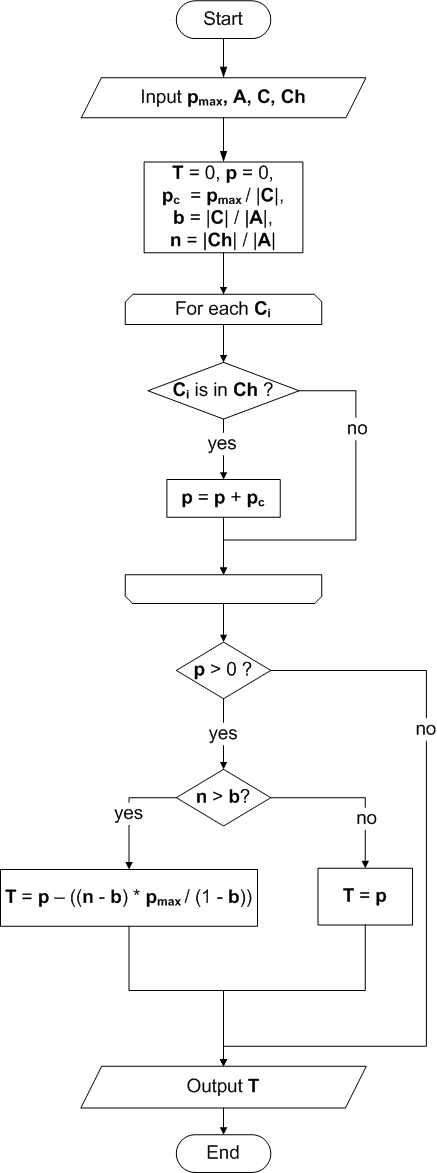
\includegraphics[width=.5\columnwidth]{images/algorithm.jpg}
	\caption{Flow chart of the Balanced scoring algorithm.}
	\label{fig:algorithm}
\end{figure}

\subsubsection{Scoring the basic points}

To score the basic points we use the approach, described by Ripkey. 
Below we present it mathematically in accordance with the following designations:

\begin{itemize}
    \item $d \in \mathbb{R} , d \in (1..d_{max}]$ -- difficulty of the current question, for our experiments we set $d_{max} = 5$ 
    \item $C \subseteq A$ -- set of the \textit{correct} options $c_i$ for the current question, where $A$ -- set of the options $a_j$ for the current question,
    \item $c_{max} = |C| , c_{max} \in \mathbb{N}$ -- number of \textit{correct} options for the current question
    \item $C_{ch}$ -- set of the \textit{correctly checked} options
    \item $c_{ch} = |C_{ch}| , c_{ch} \in \mathbb{N} , c_{ch} \in [0,c_{max}]$ -- number of \textit{correctly checked} options for the current question
    \item $p_{max} = f(d) = d*K_{points}$ -- maximal possible points for the current question, in our system we set $K_{points} = 1$
    \item $p_c$ -- points for the correctly checked option $c$. 
    As we assume all the correct options have the equal weight, 
    \[\forall c \in C_{ch} \vert p_c = \frac{p_{max}}{c_{max}}\]
    \item $p \in \mathbb{R} \wedge p \in [0,p_{max}]$ -- the basic points for the current question,
    \[p = \sum_{c \in C_{ch}}{p_c} \Rightarrow \]

   \[p = \sum_{c \in C_{ch}}{\frac{p_{max}}{c_{max}}} = \frac{p_{max}}  {c_{max}}*c_{ch} = p_c*c_{ch}\]
\end{itemize}

\subsubsection{Scoring of the penalty}

Below we present our approach for scoring the penalty.
We use the following designations:

\begin{itemize}
    \item $a_{max} \in \mathbb{N} , a_{max} = |A|$ -- number of options $a \in A$
    \item $Ch \subseteq A$ -- set of \textit{checked} options
    \item $ch = |Ch| , ch \in \mathbb{N} , ch \in [0,a_{max}]$ -- number of checked options for the current question
    \item $b \in \mathbb{R} , b \in [0,1]$ -- basic level of guessing for the current question, 
    \[b = \frac{c_{max}}{a_{max}}\]
    \item $n \in \mathbb{R} , n \in [b,1]$ -- measure, that shows the possibility, that user tries to guess the correct response by choosing too much options; we do not evaluate it in the cases, when $n <= b$,
   \[n = \frac{ch}{a_{max}}\]
    \item $s$ -- penalty for the guessing,
    \[s = n-b \Rightarrow s \in [0,1-b]\]
    \item $s_k \in [0,p_{max}]$ -- the penalty, mapped to the maximal possible points.
\end{itemize}

A mapping function is calculated as follows:
\[f : s_k \rightarrow s\]
Given, $s_k \in [0,p_{max}]$ and $s \in [0,1-b]$, then 
\[f : s_k \rightarrow s = f : [0 , {1-b}] \rightarrow [0,p_{max}] \Rightarrow\]
\[s_k = f(s) = s*\frac{p_{max}}{1-b} = (n-b)*\frac{p_{max}}{1-b}\]

\subsubsection{Scoring the total question score}

The absolute score for the question is trivially determined as
\[T = f(p,s_k) = p-s_k \]
The percentage representation of the total score is determined as follows:
\[T_\% = \frac{p - s_k}{p_{max}}*100\%\]


\section{Evaluation}
\label{sec:experiments}

\subsection{Synthetic experiments}
\label{subsec:experiment}

In the subsection we describe our experiments with synthetic data and compare the behavior of different methods.
For shorter presentation, we use the following reductions:

\begin{itemize}
  \item{Dich.} -- dichotomous scoring;
  \item{Balanced} -- the proposed balanced scoring method
\end{itemize}

We consider all the questions to have the difficulty $d = 1$, then the maximal possible points $p_{max} = 1$ as well.

\begin{table}[h!]
	\centering
%	\renewcommand{\tabcolsep}{0.15cm}
%	\renewcommand{\arraystretch}{1.3}
	\begin{tabularx}{0.5\columnwidth}{c c c c c}  
	\toprule  
    \multicolumn{5}{c}{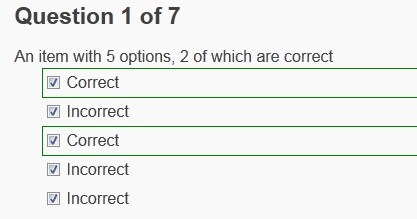
\includegraphics[width=0.5\columnwidth]{images/case1.jpg}}\\
    \midrule
    \textbf{Dich.}&\textbf{MTF}&\textbf{Morgan}&\textbf{Ripkey}&\textbf{Balanced}\\
	\midrule
    0&0.4&0&0&0\\
	\bottomrule
    \end{tabularx}
	\caption{Comparison of the proposed approach with other existing approaches}
	\label{tab:case 1}
\end{table}

\begin{example}[Case: 5 options, 2 correct, 5 marked]
In the case the student chose all the options and should obtain zero points. 
However, we see that MTF method does not recognize this type of guessing and considers the questions to be answered partially correct, awarding the points for two correct options, that were marked.
\end{example}

\begin{table}[h!]
	\centering
%	\renewcommand{\tabcolsep}{0.15cm}
%	\renewcommand{\arraystretch}{1.3}
	\begin{tabularx}{0.5\columnwidth}{c c c c c} 
	\toprule  
    \multicolumn{5}{c}{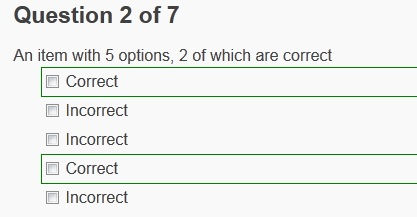
\includegraphics[width=0.5\columnwidth]{images/case2.jpg}}\\
    \midrule
    \textbf{Dich.}&\textbf{MTF}&\textbf{Morgan}&\textbf{Ripkey}&\textbf{Balanced}\\
	\midrule
    0&0.6&0&0&0\\
	\bottomrule
    \end{tabularx}
	\caption{Comparison of the proposed approach with other existing approaches}
	\label{tab:case 2}
\end{table}

\begin{example}[Case: 5 options, 2 correct, 0 marked]
The situation is opposite to the previous: in the case the student chose none of the options. 
As we assume that question must have at least one correct option, in  case of not choosing any options a student also should obtain zero points.
However, we see that MTF method awards the points for three distractors, that were not marked.
Although the situation is absurd, we faced it within real learning platforms, for example within several on-line courses of the Stanford University~\footnote{http://online.stanford.edu/courses}.
\end{example}

Two examples below are trivial and the problem could be solved by adding the rules. 
However, the MTF scoring also suffers from skewness, when applied to MMQs, as it is shown below.

\begin{table}[h!]
	\centering
%	\renewcommand{\tabcolsep}{0.15cm}
%	\renewcommand{\arraystretch}{1.3}
	\begin{tabularx}{0.5\columnwidth}{c c c c c} 
	\toprule  
    \multicolumn{5}{c}{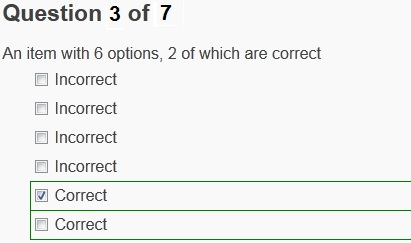
\includegraphics[width=0.5\columnwidth]{images/case3.jpg}}\\
    \midrule
    \textbf{Dich.}&\textbf{MTF}&\textbf{Morgan}&\textbf{Ripkey}&\textbf{Balanced}\\
	\midrule
    0&0.83&0.5&0.5&0.5\\
	\bottomrule
    \end{tabularx}
	\caption{Comparison of the proposed approach with other existing approaches}
	\label{tab:case 3}
\end{table}

\begin{example}[Case: 6 options, 2 correct, 1 correct marked]
This case proves, that the MTF method has a dependency from a number of correct and incorrect options. 
Thus, in a case of 6 options two of which are correct, a student is awarded 0.833 points for choosing only one correct option.
In a case of 5 options two of which are correct, she would be awarded 0.80 points for the same.
Moreover, if she choose only one incorrect option in a case of 6 alternatives, she obtains 0.5 points; in a case of 5 options she will be awarded 0.4 for the same.
\end{example}

Thus, our experiments prove, that multiple-mark questions can not be scored properly with the algorithms, developed for multiple true-false items.
Moreover, a teacher should be careful when creating multiple true-false questions and create them in such a manner, that not-choosing a distractor deserves awarding.
However, the MTF scoring is the only existing approach of partial scoring that can be used in a case, when a question does not have any correct options.

\begin{table}[h!]
	\centering
%	\renewcommand{\tabcolsep}{0.15cm}
%	\renewcommand{\arraystretch}{1.3}
	\begin{tabularx}{0.5\columnwidth}{c c c c c} 
	\toprule 
    \multicolumn{5}{c}{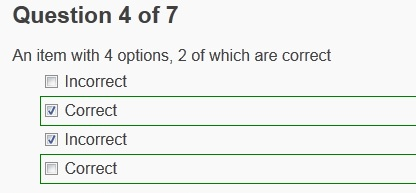
\includegraphics[width=0.5\columnwidth]{images/case4.jpg}}\\
    \midrule
    \textbf{Dich.}&\textbf{MTF}&\textbf{Morgan}&\textbf{Ripkey}&\textbf{Balanced}\\
	\midrule
    0&0.5&0&0.5&0.5\\
	\bottomrule
    \end{tabularx}
	\caption{Comparison of the proposed approach with other existing approaches}
	\label{tab:case 4}
\end{table}

\begin{example}[Case: 4 options, 2 correct, 1 correct and 1 incorrect marked]
This case illustrates the issues of using the Morgan algorithm.
The Morgan algorithm deducts penalties for choosing the incorrect option, as well as the proposed approach.
There are two main issues:

\begin{itemize}
  \item Does the response deserve penalty?
  \item If deserves, how big the penalty should be?
\end{itemize}

In that case we are facing the situation, that penalty has the same size, as the basic points, and the student is awarded zero.
We consider the penalty to be needlessly high, especially because the penalty depends on the number of incorrect options.
Thus, if the question has 3 incorrect options, choosing one of them would be fined on 0.33, and in case of 2 incorrect options, the penalty is 0.5.
After recognizing behavior of the algorithm, students will mark only the options, they are sure in, because choosing an incorrect one may cost them a full amount of points, they collected with correct options.
\end{example}

The next two examples show mainly the differences between the proposed approach and Ripkey algorithm.
Namely, we show the situations, when Ripkey algorithm awards zero points, while we consider that it should award more. 

\begin{table}[h!]
	\centering
%	\renewcommand{\tabcolsep}{0.15cm}
%	\renewcommand{\arraystretch}{1.3}
	\begin{tabularx}{0.5\columnwidth}{c c c c c} 
	\toprule  
    \multicolumn{5}{c}{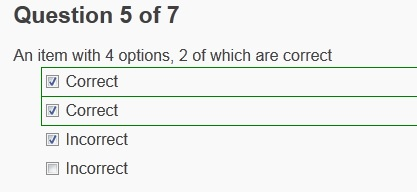
\includegraphics[width=0.5\columnwidth]{images/case5.jpg}}\\
    \midrule
    \textbf{Dich.}&\textbf{MTF}&\textbf{Morgan}&\textbf{Ripkey}&\textbf{Balanced}\\
	\midrule
    0&0.75&0.5&0&0.5\\
	\bottomrule
    \end{tabularx}
	\caption{Comparison of the proposed approach with other existing approaches}
	\label{tab:case 5}
\end{table}

\begin{example}[Case: 4 options, 2 correct, 2 correct and 1 incorrect marked]
In this case the student chose more options, than the number of correct ones, and according to the Ripkey, the answer should be awarded zero.
Our claim is, that until the student have not chosen all the options, she could have some points.
However, choosing three of four options could mean a try of guessing.
Although in this case the student gets the full amount of \textit{basic} points, she is fined on a half of them.
\end{example}

\begin{table}[h!]
	\centering
%	\renewcommand{\tabcolsep}{0.15cm}
%	\renewcommand{\arraystretch}{1.3}
	\begin{tabularx}{0.5\columnwidth}{c c c c c} 
	\toprule  
    \multicolumn{5}{c}{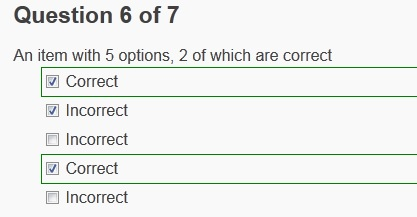
\includegraphics[width=0.5\columnwidth]{images/case6.jpg}}\\
    \midrule
    \textbf{Dich.}&\textbf{MTF}&\textbf{Morgan}&\textbf{Ripkey}&\textbf{Balanced}\\
	\midrule
    0&0.8&0.67&0&0.67\\
	\bottomrule
    \end{tabularx}
	\caption{Comparison of the proposed approach with other existing approaches}
	\label{tab:case 6}
\end{table}

\begin{example}[Case: 5 options, 2 correct, 2 correct and 1 incorrect marked]
The example shows the disadvantage of the Ripkey algorithm more clear.
It is not clear for the student, why she was awarded zero points, as she did not try to guess and answered partially correct.
\end{example}

\begin{table}[h!]
	\centering
	\begin{tabularx}{0.5\columnwidth}{c c c c c}    
    \toprule
    \multicolumn{5}{c}{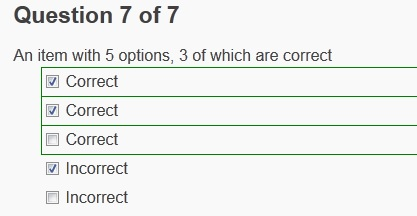
\includegraphics[width=0.5\columnwidth]{images/case7.jpg}}\\
    \midrule
    \textbf{Dich.}&\textbf{MTF}&\textbf{Morgan}&\textbf{Ripkey}&\textbf{Balanced}\\
	\midrule
    0&0.6&0.17&0.67&0.67\\
	\bottomrule
    \end{tabularx}
	\caption{Comparison of the proposed approach with other existing approaches}
	\label{tab:case 7}
\end{table}

\begin{example}[Case: 5 options, 3 correct, 2 correct and 1 incorrect marked]
In that case balanced scoring and Ripkey algorithms behave the same, as none of them deducts a penalty.
\end{example}

\section{Conclusions}
\label{sec:conclusions}

In the paper we evaluate the existing approaches for scoring the multiple-mark questions and propose a new one.
The proposed approach has a list of restrictions, however it has advantages when compare with the discussed approaches.
One of the main advantages is its clearness for the students, that was proven by the user evaluation.
Also, our approach is based on the mathematical model, it does not suffer from the skewness, as it has the same formula for all cases.
At the same time, the proposed approach recognizes the attempts to guess the correct answer, for example choosing all the possible options.
When compare with the existing approaches, the advantages of the proposed algorithm could be summarized as follows:

\begin{itemize}
  \item The approach allows to score both multiple-mark and conventional multiple-choice questions.
  \item The approach is based on the partial scoring concept.
  \item The algorithm can be easily implemented, it is pure mathematical.
  \item The score does not highly depend on the amount of correct and incorrect options.
  \item The value of the penalty is in balance with the possibility, that the student is trying to guess.
  \item Due to the balance, the results are clear for the students.  
\end{itemize}

However, we suppose our algorithm to be optional together with other discussed approaches.
This is due to the fact, that teachers create questions in their own manner and should be able to choose an appropriate method to score the results.
Also, the different situations require different levels of 	
severity, and the proposed approach might be too lenient.




%------------------------------------------------------------------------------
\chapter{RDB2RDF Mapping Documentation}
\label{sec:app1}
%------------------------------------------------------------------------------
\section{R2RML mapping representation}
\label{app1:r2rml}

\begin{lstlisting}

prefix rr: <http://www.w3.org/ns/r2rml#>.
@prefix sw: <http://slidewiki.org/rdf/sw#>.
@prefix wa: <http://slidewiki.org/rdf/wa#>.
@prefix sa: <http://slidewiki.org/rdf/sa#>.
@prefix dcterms: <http://purl.org/dc/terms/>.
@prefix foaf: <http://xmlns.com/foaf/0.1/>.
@prefix cnt: <http://www.w3.org/2011/content#>.
@prefix oa: <http://www.w3.org/ns/oa#>.

<#DeckContainerIncludes>
	rr:logicalTable [ rr:tableName "deck_revision" ];
    rr:subjectMap [
        rr:template "http://slidewiki.org/rdf/deckContainer/{deck_id}";
        rr:class sw:DeckContainer;
    ];
	rr:predicateObjectMap [
        rr:predicate wa:includes;
        rr:objectMap [
			rr:template "http://slidewiki.org/rdf/deck/{id}";			
		];
	].
	
<#DeckContainer>
    rr:logicalTable [ rr:tableName "deck" ];	
    rr:subjectMap [
        rr:template "http://slidewiki.org/rdf/deckContainer/{id}";
        rr:class sw:DeckContainer;
    ];
    rr:predicateObjectMap [
        rr:predicate dcterms:created;
        rr:objectMap [ rr:column "timestamp" ];
    ];
	rr:predicateObjectMap [
        rr:predicate dcterms:creator;
        rr:objectMap [ 
	    rr:parentTriplesMap <#User>;
            rr:joinCondition [
                rr:child "user_id";
                rr:parent "id";
            ];
		];
	];
	rr:predicateObjectMap [
        rr:predicate wa:translationOf;
        rr:objectMap [ 
			rr:template "http://slidewiki.org/rdf/deckContainer/{translated_from}";
		];
	].

<#SlideContainerIncludes>
	rr:logicalTable [ rr:tableName "slide_revision" ];
    rr:subjectMap [
        rr:template "http://slidewiki.org/rdf/slideContainer/{slide}";
        rr:class sw:SlideContainer;
    ];
	rr:predicateObjectMap [
        rr:predicate wa:includes;
        rr:objectMap [
			rr:template "http://slidewiki.org/rdf/slide/{id}";			
		];
	].
	
<#SlideContainer>
    rr:logicalTable [ rr:tableName "slide" ];
    rr:subjectMap [
        rr:template "http://slidewiki.org/rdf/slideContainer/{id}";
        rr:class sw:SlideContainer;
    ];
    rr:predicateObjectMap [
        rr:predicate dcterms:creator;
        rr:objectMap [ 
	    rr:parentTriplesMap <#User>;
            rr:joinCondition [
                rr:child "user_id";
                rr:parent "id";
            ];
		];
	];
	rr:predicateObjectMap [
        rr:predicate wa:translationOf;
        rr:objectMap [ 
			rr:template "http://slidewiki.org/rdf/slideContainer/{translated_from}";
		];
	];
	rr:predicateObjectMap [
        rr:predicate dcterms:source;
        rr:objectMap [ rr:column "description" ];
	].
	
	

<#TagDeck>
	rr:logicalTable [ rr:sqlQuery """
	SELECT *
	FROM tag WHERE tag.item_type='deck' """ 
	];
    rr:subjectMap [
        rr:template "http://slidewiki.org/rdf/deck/{item_id}";
        rr:class sw:Deck;
    ];
	rr:predicateObjectMap [
        rr:predicate dcterms:subject;
        rr:objectMap [ rr:column "tag" ];
	].
	
<#DeckPartOf>
	rr:logicalTable [ rr:sqlQuery """
	SELECT *
	FROM deck_content WHERE deck_content.item_type='deck'""" 
	];
    rr:subjectMap [
        rr:template "http://slidewiki.org/rdf/deck/{item_id}";
        rr:class sw:Deck;
    ];
	rr:predicateObjectMap [
        rr:predicate dcterms:isPartOf;
        rr:objectMap [
			rr:template "http://slidewiki.org/rdf/deck/{deck_revision_id}"
		];
	].

<#SlidePartOf>
	rr:logicalTable [ rr:sqlQuery """
	SELECT *
	FROM deck_content WHERE deck_content.item_type='slide'""" 
	];
    rr:subjectMap [
        rr:template "http://slidewiki.org/rdf/slide/{item_id}";
        rr:class sw:Slide;
    ];
	rr:predicateObjectMap [
        rr:predicate dcterms:isPartOf;
        rr:objectMap [ 
			rr:template "http://slidewiki.org/rdf/deck/{deck_revision_id}";
		];
	].
	

<#DeckHasPartDecks>
	rr:logicalTable [ rr:sqlQuery """
	SELECT *
	FROM deck_content WHERE deck_content.item_type='deck'""" 
	];
    rr:subjectMap [
        rr:template "http://slidewiki.org/rdf/deck/{deck_revision_id}";
        rr:class sw:Deck;
    ];
	rr:predicateObjectMap [
        rr:predicate dcterms:hasPart;
        rr:objectMap [ 
			rr:template "http://slidewiki.org/rdf/deck/{item_id}";
		];
	].
	
<#DeckHasPartSlides>
	rr:logicalTable [ rr:sqlQuery """
	SELECT *
	FROM deck_content WHERE deck_content.item_type='slide'""" 
	];
    rr:subjectMap [
        rr:template "http://slidewiki.org/rdf/deck/{deck_revision_id}";
        rr:class sw:Deck;
    ];
	rr:predicateObjectMap [
        rr:predicate dcterms:hasPart;
        rr:objectMap [ 
			rr:template "http://slidewiki.org/rdf/slide/{item_id}";
		];
	].
	
	
<#DeckContributor>
	rr:logicalTable [ rr:sqlQuery """
	SELECT deck_revision.id, deck_revision.user_id as deck_user, user_group.user_id as user_user, user_group.deck_revision_id
	FROM deck_revision
	JOIN user_group ON deck_revision.id = user_group.deck_revision_id
	WHERE user_group.user_id != deck_revision.user_id """ 
	];
    rr:subjectMap [
        rr:template "http://slidewiki.org/rdf/deck/{id}";
        rr:class sw:Deck;
    ];
	rr:predicateObjectMap [
        rr:predicate dcterms:contributor;
        rr:objectMap [ 
			rr:parentTriplesMap <#User>;
            rr:joinCondition [
                rr:child "user_user";
                rr:parent "id";
            ];
		];		
	].
	

<#Deck>
    rr:logicalTable [ rr:sqlQuery """
	SELECT deck.language, deck_revision.*
	FROM deck
	JOIN deck_revision ON deck_revision.deck_id = deck.id """
	];
    rr:subjectMap [
        rr:template "http://slidewiki.org/rdf/deck/{id}";
        rr:class sw:Deck;
    ];
    rr:predicateObjectMap [
        rr:predicate dcterms:created;
        rr:objectMap [ rr:column "timestamp" ];
    ];
	rr:predicateObjectMap [
        rr:predicate dcterms:language;
        rr:objectMap [ rr:column "language" ];
    ];
    rr:predicateObjectMap [
        rr:predicate dcterms:title;
        rr:objectMap [ rr:column "title" ];
    ];    
    rr:predicateObjectMap [
        rr:predicate sw:popularity;
        rr:objectMap [ rr:column "popularity" ];
    ];
    rr:predicateObjectMap [
        rr:predicate dcterms:description;
        rr:objectMap [ rr:column "abstract" ];
    ];
    rr:predicateObjectMap [
        rr:predicate wa:instanceOf;
        rr:objectMap [ 
	    rr:parentTriplesMap <#DeckContainer>;
            rr:joinCondition [
                rr:child "deck_id";
                rr:parent "id";
            ];
		];
    ];
	rr:predicateObjectMap [
        rr:predicate dcterms:creator;
        rr:objectMap [ 
	    rr:parentTriplesMap <#User>;
            rr:joinCondition [
                rr:child "user_id";
                rr:parent "id";
            ];
		];
	];
	rr:predicateObjectMap [
        rr:predicate dcterms:contributor;
        rr:objectMap [ 
	    rr:parentTriplesMap <#User>;
            rr:joinCondition [
                rr:child "user_id";
                rr:parent "id";
            ];
		];
	];
	rr:predicateObjectMap [
        rr:predicate wa:translationOf;
        rr:objectMap [ 
			rr:template "http://slidewiki.org/rdf/deck/{translated_from_revision}";
		];
	];
	rr:predicateObjectMap [
        rr:predicate wa:revisionOf;
        rr:objectMap [ 
			rr:template "http://slidewiki.org/rdf/deck/{based_on}";
		];
	];
	rr:predicateObjectMap [
        rr:predicate oa:styledBy;
        rr:objectMap [ 
			rr:template "http://slidewiki.org/rdf/style/{default_theme}";
		];
	].
	
<#Slide>
    rr:logicalTable [ rr:sqlQuery """
	SELECT slide.language, slide_revision.*
	FROM slide
	JOIN slide_revision ON slide_revision.slide = slide.id """
	];
    rr:subjectMap [
        rr:template "http://slidewiki.org/rdf/slide/{id}";
        rr:class sw:Slide
    ];
    rr:predicateObjectMap [
        rr:predicate dcterms:created;
        rr:objectMap [ rr:column "timestamp" ];
    ];
	rr:predicateObjectMap [
        rr:predicate dcterms:language;
        rr:objectMap [ rr:column "language" ];
    ];
    rr:predicateObjectMap [
        rr:predicate cnt:chars;
        rr:objectMap [ rr:column "content" ];
    ];    
    rr:predicateObjectMap [
        rr:predicate sw:popularity;
        rr:objectMap [ rr:column "popularity" ];
    ];
    rr:predicateObjectMap [
        rr:predicate dcterms:description;
        rr:objectMap [ rr:column "comment" ];
    ];
	rr:predicateObjectMap [
        rr:predicate sw:slideNote;
        rr:objectMap [ rr:column "note" ];
    ];
    rr:predicateObjectMap [
        rr:predicate wa:instanceOf;
        rr:objectMap [ 
	    rr:parentTriplesMap <#SlideContainer>;
            rr:joinCondition [
                rr:child "slide";
                rr:parent "id";
            ];
		];
    ];
	rr:predicateObjectMap [
        rr:predicate dcterms:creator;
        rr:objectMap [ 
	    rr:parentTriplesMap <#User>;
            rr:joinCondition [
                rr:child "user_id";
                rr:parent "id";
            ];
		];
	];
	rr:predicateObjectMap [
        rr:predicate sw:translator;
        rr:objectMap [ 
	    rr:parentTriplesMap <#User>;
            rr:joinCondition [
                rr:child "translator_id";
                rr:parent "id";
            ];
		];
	];
	rr:predicateObjectMap [
        rr:predicate wa:translationOf;
        rr:objectMap [ 
			rr:template "http://slidewiki.org/rdf/slide/{translated_from_revision}";
		];
	];
	rr:predicateObjectMap [
        rr:predicate wa:revisionOf;
        rr:objectMap [ 
			rr:template "http://slidewiki.org/rdf/slide/{based_on}";
		];
	].
	
	
<#QuestionsAssigned>
	rr:logicalTable [ rr:sqlQuery """
	SELECT *
	FROM questions WHERE questions.id NOT IN
	(SELECT `based_on` FROM `questions` WHERE based_on IS NOT NULL)"""
	];
    rr:subjectMap [
        rr:template "http://slidewiki.org/rdf/question/{id}";
        rr:class sw:Queston;
    ];
    rr:predicateObjectMap [
        rr:predicate wa:assignedTo;
        rr:objectMap [ 
			rr:template "http://slidewiki.org/rdf/slideContainer/{item_id}";
		];
    ].
	
<#CommentDecks>
	rr:logicalTable [ rr:sqlQuery """ 
	SELECT * FROM comment
	WHERE item_type='deck'
	"""];
	rr:subjectMap [
        rr:template "http://slidewiki.org/rdf/comment/{id}";
        rr:class sw:Comment;
    ];
	rr:predicateObjectMap [
        rr:predicate wa:assignedTo;
        rr:objectMap [ 
			rr:template "http://slidewiki.org/rdf/deck/{item_id}";
		];
    ];
	rr:predicateObjectMap [
        rr:predicate dcterms:creator;
        rr:objectMap [ 
	    rr:parentTriplesMap <#User>;
            rr:joinCondition [
                rr:child "user_id";
                rr:parent "id";
            ];
		];
	];
	rr:predicateObjectMap [
        rr:predicate cnt:chars;
        rr:objectMap [ rr:column "text" ];
    ];
	rr:predicateObjectMap [
        rr:predicate dcterms:title;
        rr:objectMap [ rr:column "title" ];
    ];
	rr:predicateObjectMap [
        rr:predicate dcterms:created;
        rr:objectMap [ rr:column "timestamp" ];
    ].

<#CommentSlides>
	rr:logicalTable [ rr:sqlQuery """ 
	SELECT * FROM comment
	WHERE item_type='slide'
	"""];
	rr:subjectMap [
        rr:template "http://slidewiki.org/rdf/comment/{id}";
        rr:class sw:Comment;
    ];
	rr:predicateObjectMap [
        rr:predicate wa:assignedTo;
        rr:objectMap [ 
			rr:template "http://slidewiki.org/rdf/slide/{item_id}";
		];
    ];
	rr:predicateObjectMap [
        rr:predicate dcterms:creator;
        rr:objectMap [ 
	    rr:parentTriplesMap <#User>;
            rr:joinCondition [
                rr:child "user_id";
                rr:parent "id";
            ];
		];
	];
	rr:predicateObjectMap [
        rr:predicate cnt:chars;
        rr:objectMap [ rr:column "text" ];
    ];
	rr:predicateObjectMap [
        rr:predicate dcterms:title;
        rr:objectMap [ rr:column "title" ];
    ];
	rr:predicateObjectMap [
        rr:predicate dcterms:created;
        rr:objectMap [ rr:column "timestamp" ];
    ].
	
	
<#StyleHasRevision>
	rr:logicalTable [ rr:sqlQuery """
	SELECT * FROM style
	WHERE based_on IS NOT NULL
	"""];
	rr:subjectMap [
		rr:template "http://slidewiki.org/rdf/style/{based_on}";
        rr:class sw:Style
	];
	rr:predicateObjectMap [
		rr:predicate wa:hasRevision;
		rr:objectMap[ 
			rr:template  "http://slidewiki.org/rdf/style/{id}";                
        ];
	];
	rr:predicateObjectMap [
        rr:predicate dcterms:creator;
        rr:objectMap [ 
	    rr:parentTriplesMap <#User>;
            rr:joinCondition [
                rr:child "user_id";
                rr:parent "id";
            ];
		];
	].
	

<#Style>
	rr:logicalTable [ rr:tableName "style" ];
    rr:subjectMap [
        rr:template "http://slidewiki.org/rdf/style/{id}";
        rr:class sw:Style;
    ];
	rr:predicateObjectMap [
        rr:predicate dcterms:created;
        rr:objectMap [ rr:column "timestamp" ];
    ];
	rr:predicateObjectMap [
        rr:predicate cnt:chars;
        rr:objectMap [ rr:column "css" ];
    ];
	rr:predicateObjectMap [
        rr:predicate dcterms:description;
        rr:objectMap [ rr:column "comment" ];
    ];
	rr:predicateObjectMap [
        rr:predicate dcterms:title;
        rr:objectMap [ rr:column "name" ];
    ];
	rr:predicateObjectMap [
        rr:predicate dcterms:creator;
        rr:objectMap [ 
	    rr:parentTriplesMap <#User>;
            rr:joinCondition [
                rr:child "user_id";
                rr:parent "id";
            ];
		];
	];
	rr:predicateObjectMap [
        rr:predicate wa:revisionOf;
		rr:objectMap[ 
			rr:template  "http://slidewiki.org/rdf/style/{based_on}";                
        ];
	].
	
	
	
	
<#Question>
	rr:logicalTable [ rr:tableName "questions" ];
    rr:subjectMap [
        rr:template "http://slidewiki.org/rdf/question/{id}";
        rr:class sw:Queston;
		rr:class sa:Queston;
    ];
	rr:predicateObjectMap [
        rr:predicate dcterms:created;
        rr:objectMap [ rr:column "timestamp" ];
    ];
    rr:predicateObjectMap [
        rr:predicate sw:defaultDifficulty;
        rr:objectMap [ rr:column "difficulty" ];
    ];
	rr:predicateObjectMap [
        rr:predicate cnt:chars;
        rr:objectMap [ rr:column "question" ];
    ];
	rr:predicateObjectMap [
        rr:predicate sa:difficultyLevel;
        rr:objectMap [ rr:column "diff_count" ];
    ];
	rr:predicateObjectMap [
        rr:predicate wa:revisionOf;
        rr:objectMap [ 
			rr:template "http://slidewiki.org/rdf/question/{based_on}";
		];
	];
	rr:predicateObjectMap [
        rr:predicate dcterms:creator;
        rr:objectMap [ 
	    rr:parentTriplesMap <#User>;
            rr:joinCondition [
                rr:child "user_id";
                rr:parent "id";
            ];
		];
	].
	
	


<#UserTestHasPart>
	rr:logicalTable [rr:tableName "test_content"];
	rr:subjectMap [
		rr:template "http://slidewiki.org/rdf/userTest/{test_id}";
        rr:class sw:UserTest;
	];
	rr:predicateObjectMap [
        rr:predicate dcterms:hasPart;
        rr:objectMap [ 
			rr:parentTriplesMap <#Question>;
			rr:joinCondition [
				rr:child "question_id";
				rr:parent "id";
			];
		];		
    ].
	
<#QuestionPartOftest>
	rr:logicalTable [rr:tableName "test_content"];
	rr:subjectMap [
		rr:template "http://slidewiki.org/rdf/question/{question_id}";
        rr:class sw:Question;		
	];
	rr:predicateObjectMap [
        rr:predicate dcterms:isPartOf;
        rr:objectMap [ 
			rr:parentTriplesMap <#UserTest>;
			rr:joinCondition [
				rr:child "test_id";
				rr:parent "id";
			];
		];		
    ].	
	
<#Choice>
	rr:logicalTable [ rr:tableName "answers"];
	rr:subjectMap [
		rr:template "http://slidewiki.org/rdf/choice/{id}";
        rr:class sa:Choice;
	];
	rr:predicateObjectMap [
        rr:predicate cnt:chars;
        rr:objectMap [ rr:column "answer" ];
    ];
	rr:predicateObjectMap [
        rr:predicate sa:explanation;
        rr:objectMap [ rr:column "explanation" ];
    ].
	
<#Distractors>
	rr:logicalTable [ rr:sqlQuery """
		SELECT * 
		FROM answers
		WHERE is_right='no' """
	];
	rr:subjectMap [
		rr:template "http://slidewiki.org/rdf/question/{question_id}";
        rr:class sw:Question;
	];
	rr:predicateObjectMap [
        rr:predicate sa:distractor;
        rr:objectMap [ 
			rr:parentTriplesMap <#Choice>;
			rr:joinCondition [
				rr:child "id";
				rr:parent "id";
			];
		];
    ].
	
<#CorrectChoices>
	rr:logicalTable [ rr:sqlQuery """
		SELECT * 
		FROM answers
		WHERE is_right='yes' """
	];
	rr:subjectMap [
		rr:template "http://slidewiki.org/rdf/question/{question_id}";
        rr:class sw:Question;
	];
	rr:predicateObjectMap [
        rr:predicate sa:correctChoice;
        rr:objectMap [ 
			rr:parentTriplesMap <#Choice>;
			rr:joinCondition [
				rr:child "id";
				rr:parent "id";
			];
		];
    ].
	
<#UserTest>
	rr:logicalTable [ rr:tableName "user_tests" ];
    rr:subjectMap [
        rr:template "http://slidewiki.org/rdf/userTest/{id}";
        rr:class sw:UserTest;
    ];
	rr:predicateObjectMap [
        rr:predicate dcterms:created;
        rr:objectMap [ rr:column "timestamp" ];
    ];
	rr:predicateObjectMap [
        rr:predicate dcterms:title;
        rr:objectMap [ rr:column "title" ];
    ];
	rr:predicateObjectMap [
        rr:predicate dcterms:creator;
        rr:objectMap [ 
			rr:parentTriplesMap <#User>;
            rr:joinCondition [
                rr:child "user_id";
                rr:parent "id";
            ];
		];
	].

<#User>
    rr:logicalTable [ rr:tableName "users" ];
    rr:subjectMap [
        rr:template "http://slidewiki.org/rdf/user/{id}";
        rr:class sw:User;
    ];
    rr:predicateObjectMap [
        rr:predicate foaf:mbox;
        rr:objectMap [ rr:column "email" ];
    ];
    rr:predicateObjectMap [
        rr:predicate foaf:nick;
        rr:objectMap [ rr:column "username" ];
    ];
    rr:predicateObjectMap [
        rr:predicate dcterms:date;
        rr:objectMap [ rr:column "registered" ];
    ];
    rr:predicateObjectMap [
        rr:predicate foaf:firstName;
        rr:objectMap [ rr:column "first_name" ];
    ];
    rr:predicateObjectMap [
        rr:predicate foaf:familyName;
        rr:objectMap [ rr:column "last_name" ];
    ];
	rr:predicateObjectMap [
        rr:predicate dcterms:language;
        rr:objectMap [ rr:column "locale" ];
    ];
	rr:predicateObjectMap [
        rr:predicate foaf:gender;
        rr:objectMap [ rr:column "gender" ];
    ];
	rr:predicateObjectMap [
        rr:predicate sw:speaks;
        rr:objectMap [ rr:column "languages" ];
    ];
	rr:predicateObjectMap [
        rr:predicate foaf:based_near;
        rr:objectMap [ rr:column "location" ];
    ];
	rr:predicateObjectMap [
        rr:predicate foaf:topic_interest;
        rr:objectMap [ rr:column "interests" ];
    ];
	rr:predicateObjectMap [
        rr:predicate foaf:depiction;
        rr:objectMap [ rr:column "picture" ];
    ];
	rr:predicateObjectMap [
        rr:predicate sw:homeLocation;
        rr:objectMap [ rr:column "hometown" ];
    ];
	rr:predicateObjectMap [
        rr:predicate foaf:birthday;
        rr:objectMap [ rr:column "birthday" ];
    ];
	rr:predicateObjectMap [
        rr:predicate dcterms:description;
        rr:objectMap [ rr:column "description" ];
    ];
	rr:predicateObjectMap [
        rr:predicate foaf:page;
        rr:objectMap [ rr:column "infodeck" ];
    ].
    
\end{lstlisting}

%\section{Tabular mapping representation}
%
%\begin{figure}[!b]
%	\centering
%		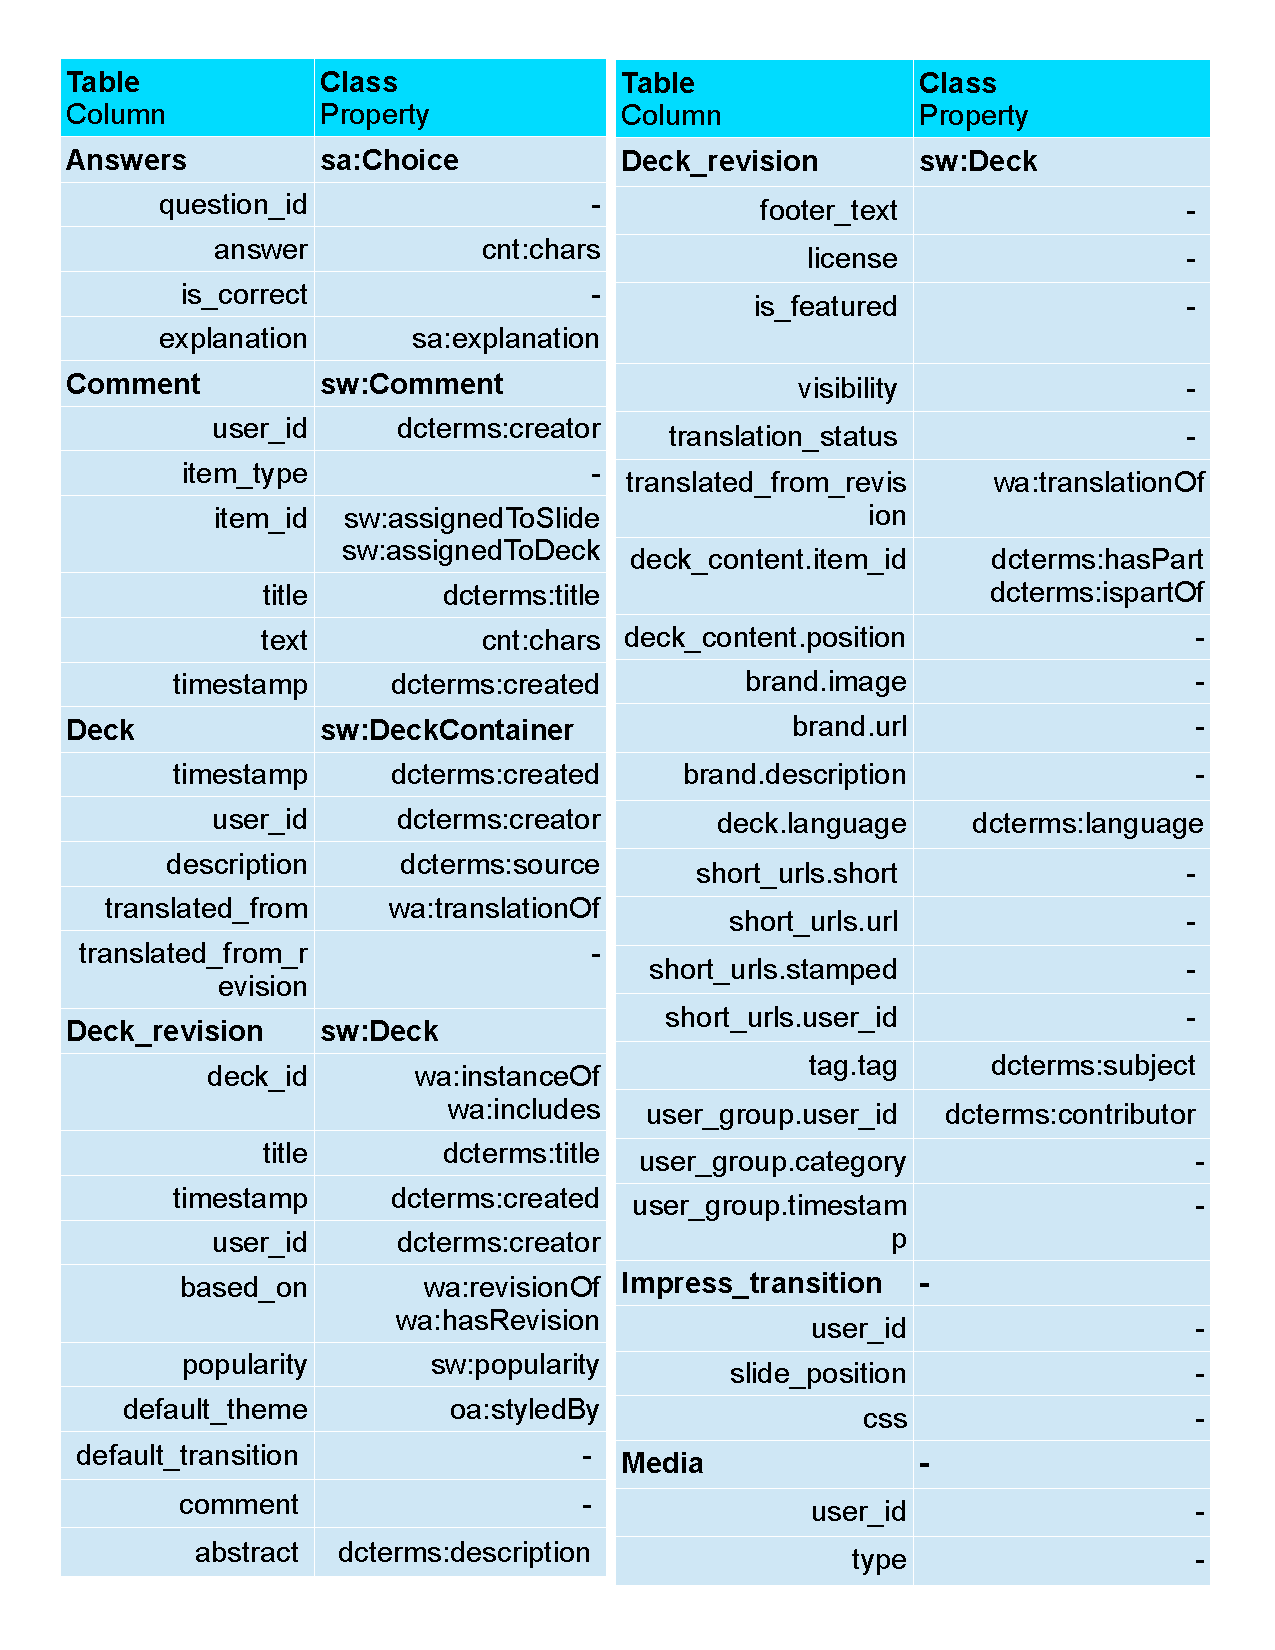
\includegraphics[width=\columnwidth]{images/mapping_pages1.pdf}
%		\caption{Matching the DB tables and columns to WikiApp ontologie classes and properties}
%	\label{fig:wa_matching_1}
%\end{figure}
%
%\begin{figure}[!b]
%	\centering
%		\includegraphics[width=\columnwidth]{images/mapping_pages2.pdf}
%		\caption{Matching the DB tables and columns to WikiApp ontologie classes and properties (cont.)}
%	\label{fig:wa_matching_2}
%\end{figure}
%
%\begin{figure}[!b]
%	\centering
%		\includegraphics[width=\columnwidth]{images/mapping_pages3.pdf}
%		\caption{Matching the DB tables and columns to WikiApp ontologie classes and properties (cont.)}
%	\label{fig:wa_matching_3}
%\end{figure}


\section{SlideWiki knowledge graph}


\begin{sidewaysfigure}[b]
    \centering
    \includegraphics[width=\columnwidth]{images/knowledge_graph.png}
    \caption{SlideWiki Knowledge graph}
	\label{fig:knowledge_graph}
\end{sidewaysfigure}






\backmatter

 {\raggedright
   \bibliographystyle{plainnat}

   \bibliography{../refs/thesis,../refs/standard_refs-bibtex,../refs/literature_review,../refs/mypub}
}

\listoffigures
\listoftables

%------------------------------------------------------------------------------
% Print the glossary and list of acronyms
% \printglossaries

%------------------------------------------------------------------------------
% CV needed when you submit your PhD thesis
%
% \definecolor{lightgray}{gray}{0.8}
\newcolumntype{L}{>{\raggedleft}p{0.15\textwidth}}
\newcolumntype{R}{p{0.8\textwidth}}
\newcommand\VRule{\color{lightgray}\vrule width 0.5pt}

\thispagestyle{empty}
\section*{Curriculum Vitae}

\subsection*{Personal Details}

\begin{tabular}{L!{\VRule}R}
Name & Johann Schmidt \\
Date of Birth &  \\
Email & abc@physik.uni-def.de \\
Family status & Single
\end{tabular}

\subsection*{Education}

\begin{tabular}{L!{\VRule}R}
1997--2003 & Abitur, ABC Secondary School, Hamburg, Germany\\
2004--2007 & BSc in Physics, Rheinische Friedrich-Wilhelms-Universität, Bonn, Germany.\\
2006 & CERN Summer Student, Geneva, Switzerland. \\
2007--2009 &  MSc in Physics Rheinische Friedrich-Wilhelms-Universität, Bonn, Germany. \\
2009--2012 &  PhD in Physics, Rheinische Friedrich-Wilhelms-Universität, Bonn, Germany. \\
2012 & Advanced Data Analysis School, Frankfurt, Germany.
\end{tabular}

\subsection*{Professional Experience}

\begin{tabular}{L!{\VRule}R}
2004 & Summer Student at CERN, Geneva, Switzerland. \\
2007--2012 & Doctoral work at the University of Bonn, Germany. \\
2008--2009 & Fieldwork at CERN, Geneva, Switzerland.\\
2011 & Talk at the Advanced Physics Conference, Timbucto
\end{tabular}

\subsection*{Languages}
\begin{tabular}{L!{\VRule}R}
German & Mother tongue \\
English & Fluent \\
Russian & Basic
\end{tabular}


\end{document}

